% !TeX program = xelatex
\documentclass[notheorems,aspectratio=1610,t]{beamer}
% The presentation template lives in the sibling Wildcat repository.
\def\wildcatlanguage{persian}
\input{.wildcat/config/preamble.tex}

% Set paragraph alignment after the shared proof's list has been initialized.
% Patch its optional-argument implementation, preserving the shared RTL/QED
% handling and the usual centered display equations.
\expandafter\apptocmd\csname\string\proof\endcsname
  {\raggedleft\ignorespaces}{}
  {\PackageError{algebra}{Cannot set Persian proof alignment}
    {Check the shared Wildcat proof environment.}}

\setlatintextfont[Extension=.otf,UprightFont=*-regular,ItalicFont=*-italic,
  BoldFont=*-bold,BoldItalicFont=*-bolditalic,
  SmallCapsFont=lmromancaps10-regular]{lmroman10}
\setmathfont{latinmodern-math.otf}
\setbeamerfont{title}{family=\fontspec{XB Roya},series=\bfseries,size=\LARGE}
\setbeamerfont{frametitle}{family=\fontspec{XB Roya},series=\bfseries,size=\large}
\setbeamerfont{section}{family=\fontspec{XB Roya},series=\bfseries,size=\LARGE}
\tikzset{wildcat cover text/.append style={text width=0.72\paperwidth}}


\title{جبر پیشرفته}
\subtitle{دانشگاه صنعتی امیرکبیر}
\author{مدرس: دکتر خسروی}
\date{}
\titlegraphic{\includegraphics[width=1.9cm]{.wildcat/assets/Aut-logo_en-white.png}}

\begin{document}
\small
\begin{frame}
  \titlepage
\end{frame}
% The lecture helper defines this only for an isolated per-PDF preview.
\ifdefined\AlgebraLectureNumber
  \setcounter{section}{\numexpr\AlgebraLectureNumber-1\relax}
  \input{sections/section\AlgebraLectureNumber.tex}
\else
  % Select the lecture content here. Each source contains frames only.


\section{ مرور جبر کارشناسی}

\begin{frame}[t]{نیم‌گروه و عمل شرکت‌پذیر}
    \begin{definition}[  نیم‌گروه]
        فرض کنید \( S \) مجموعه‌ای ناتهی باشد و یک عمل دوتایی \(\cdot\) روی \( S \) را در نظر بگیرید.
        اگر این عمل شرکت‌پذیر باشد یعنی:
        \[
            \forall a, b, c \in S \quad (a \cdot b) \cdot c = a \cdot (b \cdot c)
        \]
        آنگاه \( S \) را همراه با عمل \(\cdot\) یک \textbf{نیم‌گروه \LTRfootnote{Semigroup}} می‌نامند.

    \end{definition}


\end{frame}

\begin{frame}[t]{گروه و اصول آن}
    \begin{definition}[گروه]
        فرض کنید مجموعه ناتهی \( G \) همراه با عمل دوتایی \(\cdot\) در شرایط زیر صدق کند:
        \[\forall a, b, c \in G \quad a \cdot (b \cdot c) = (a \cdot b) \cdot c\]
        \[\exists e \in G \; \forall a \in G \quad a \cdot e = e \cdot a = a \quad \text{(وجود عنصر همانی)}\]
        \[\forall a \in G \; \exists b \in G \quad a \cdot b = b \cdot a = e \quad \text{(وجود عنصر وارون)}\]
        در این صورت \( (G, \cdot) \) را یک \textbf{گروه} می‌نامند.

    \end{definition}
    \begin{remark}
        غالبا  بجای \( a \cdot b \) می‌نویسیم \( ab \).

    \end{remark}
\end{frame}

\begin{frame}[t]{گروه آبلی و زیرگروه}
    \begin{definition}[  گروه آبلی]
        اگر به ازای هر \( a, b \in G \) داشته باشیم:
        \[
            a \cdot b = b \cdot a
        \]
        گروه را \textbf{آبلی یا جابجایی} می‌نامند.
    \end{definition}


    \begin{definition}[  زیرگروه]
        اگر \( (G, \cdot) \) یک گروه باشد و \( H \subseteq G \) زیرمجموعه‌ای ناتهی از \( G \) باشد که خودش نیز تحت عمل \(\cdot\) یک گروه باشد، آنگاه \( H \) را یک \textbf{زیرگروه} \( G \) می‌نامند و می‌نویسیم:
        \[
            H \leq G
        \]

    \end{definition}
\end{frame}

\begin{frame}[t]{محک فشردهٔ زیرگروه}
    \begin{theorem}[  محک فشرده]

        زیرمجموعه ناتهی \( H \subseteq G \) زیرگروه \( G \) است اگر و تنها اگر:
        \[
            \forall a, b \in H \quad a \cdot b^{-1} \in H
        \]
    \end{theorem}
    \begin{example}
        \( (\mathbb{Z}, +) \)، گروه اعداد صحیح با عمل جمع را در نظر بگیرید.
        زیرمجموعه‌ی \( 2\mathbb{Z} = \{ 2k \mid k \in \mathbb{Z} \} \) یعنی اعداد زوج، با همان عمل جمع، یک زیرگروه از \( \mathbb{Z} \) است، بنابراین:
        \[
            (2\mathbb{Z}, +) \leq (\mathbb{Z}, +)
        \]
    \end{example}

    \end{frame}

\begin{frame}[t]{اثبات محک زیرگروه در اعداد صحیح}
    \begin{proof}
        برای اثبات اینکه \( (2\mathbb{Z}, +) \) زیرگروه است، از محک فشرده استفاده می‌کنیم:
        باید نشان دهیم اگر \( a, b \in 2\mathbb{Z} \) باشند، آنگاه \( a - b \in 2\mathbb{Z} \).
        ازآنجا که \( a = 2m \) و \( b = 2n \)  به ازای \( m, n \in \mathbb{Z} \)، آنگاه:
        \[
            a - b = 2m - 2n = 2(m - n)
        \]
        که چون \( m - n \in \mathbb{Z} \)، پس \( a - b \in 2\mathbb{Z} \).
        بنابراین، \( a + (-b) \in 2\mathbb{Z} \) و با استفاده از محک فشرده نتیجه می‌گیریم که \( (2\mathbb{Z}, +) \) زیرگروه \( (\mathbb{Z}, +) \) است.
    \end{proof}
\end{frame}



\begin{frame}[t]{زیرگروه‌های گروه اعداد صحیح}
    \begin{example}
        \( (\mathbb{Z}, +) \)، گروه اعداد صحیح با عمل جمع را در نظر بگیرید.
        برای هر \( n \in \mathbb{N} \)، مجموعه \( n\mathbb{Z} = \{ nk \mid k \in \mathbb{Z} \} \) با همان عمل جمع، زیرگروه \( \mathbb{Z} \) است:
        \[
            (n\mathbb{Z}, +) \leq (\mathbb{Z}, +)
        \]
    \end{example}

    \begin{proof}
        برای \( a, b \in n\mathbb{Z} \)، داریم \( a = nk \)، \( b = nl \)  به ازای \( k, l \in \mathbb{Z} \)، پس:
        \[
            a - b = nk - nl = n(k - l) \in n\mathbb{Z}
        \]
        بنابراین، \( n\mathbb{Z} \) تحت تفاضل بسته است و زیرگروه \( \mathbb{Z} \) می‌باشد.
    \end{proof}
\end{frame}

\begin{frame}[t]{چرا اعداد طبیعی گروه ضربی نیستند؟}
    \begin{example}
        \( (\mathbb{N}, \times) \) گروه نیست.

        زیرا برای مثال عدد \( 2 \in \mathbb{N} \) هیچ عضو معکوسی نسبت به ضرب در \( \mathbb{N} \) ندارد.
        یعنی عدد طبیعی‌ای وجود ندارد که \( 2 \times x = 1 \) را برآورده کند.

        بنابراین، شرط وجود عنصر معکوس برای همه اعضا برقرار نیست و \( (\mathbb{N}, \times) \) گروه نیست.
    \end{example}


\end{frame}

\begin{frame}[t]{گروه ضربی یک میدان}
    \begin{definition}
        برای هر میدان \( F \)، مجموعه‌ی \( F^* \) به صورت زیر تعریف می‌شود:
        \[
            F^* = F \setminus \{0\}
        \]
        یعنی مجموعه‌ی تمام اعضای ناصفر \( F \). این مجموعه تحت عمل ضرب، یک گروه تشکیل می‌دهد.

        به طور خاص:
        \begin{itemize}
            \item \( \mathbb{Q}^* = \mathbb{Q} \setminus \{0\} \): اعداد گویا ناصفر
            \item \( \mathbb{R}^* = \mathbb{R} \setminus \{0\} \): اعداد حقیقی ناصفر
            \item \( \mathbb{C}^* = \mathbb{C} \setminus \{0\} \): اعداد مختلط ناصفر
        \end{itemize}
        هر یک از این مجموعه‌ها با عمل ضرب، یک گروه ضربی می‌سازند.
    \end{definition}
\end{frame}

\begin{frame}[t]{ماتریس‌ها به‌عنوان ساختار جبری}
    \begin{definition}
        اگر \( F \) یک میدان \LTRfootnote{Field} باشد، آنگاه \( M_n(F) \) مجموعه‌ی تمام ماتریس‌های \( n \times n \) با درایه‌هایی از \( F \) است:
        \[
            M_n(F) = \{ A = (a_{ij}) \mid 1 \leq i, j \leq n,\; a_{ij} \in F \}
        \]
        روی \( M_n(F) \) می‌توان اعمال مختلفی تعریف کرد، مانند جمع ماتریسی و ضرب ماتریسی.

        معمولاً \( (M_n(F), +) \) یک گروه آبلی است (نسبت به جمع ماتریسی) و \( (M_n(F), \cdot) \) یک نیم‌گروه است (نسبت به ضرب ماتریسی، ولی بسته به \( F \) و \( n \) ممکن است گروه نباشد زیرا ماتریس‌های ناتبدیل وارون ندارند).
    \end{definition}


\end{frame}

\begin{frame}[t]{نمونه‌هایی از زیرگروه‌ها}
    \begin{example}
        در ادامه چند مثال از زیرگروه‌ها آورده شده است:
        \begin{align*}
            (\mathbb{Z}, +)       & \leq (\mathbb{Q}, +)       \\
            (\mathbb{Q}, +)       & \leq (\mathbb{R}, +)       \\
            (\mathbb{Q}^*, \cdot) & \leq (\mathbb{R}^*, \cdot) \\
            (M_n(\mathbb{Q}), +)  & \leq (M_n(\mathbb{R}), +)  \\
        \end{align*}
    \end{example}
    \end{frame}

\begin{frame}[t]{نمونه‌هایی از گروه‌ها}
    \begin{example}[گروه]
        مثال‌هایی از گروه
        \begin{align*}
            (\mathbb{C}, +)       & \quad \text{(گروه جمعی اعداد مختلط)}                        \\
            (\mathbb{C}^*, \cdot) & \quad \text{(گروه ضربی اعداد مختلط ناصفر)}                  \\
            (M_n(\mathbb{C}), +)  & \quad \text{(گروه ماتریس‌های \( n \times n \) مختلط با جمع)}
        \end{align*}
    \end{example}
\end{frame}

\begin{frame}[t]{گروه باقیمانده‌های پیمانه‌ای}
    \begin{definition}
        برای عدد صحیح \( n \geq 2 \)، مجموعه‌ی باقیمانده‌های صحیح پیمانه‌ای را به صورت زیر تعریف می‌کنیم:
        \[
            \mathbb{Z}_n = \{ \overline{0}, \overline{1}, \overline{2}, \ldots, \overline{n-1} \}
        \]
        که در آن \( \overline{a} \) نمایانگر کلاس پیمانه‌ای \( a \) نسبت به \( n \) است، یعنی:
        \[
            \overline{a} = \{ b \in \mathbb{Z} \mid b \equiv a \pmod{n} \}
        \]

        عمل جمع روی \( \mathbb{Z}_n \) به صورت زیر تعریف می‌شود:
        \[
            \overline{i} + \overline{j} := \overline{i + j}
        \]

        به این ترتیب، \( (\mathbb{Z}_n, +) \) یک گروه آبلی متناهی است.
    \end{definition}


\end{frame}

\begin{frame}[t]{خوش‌تعریفی جمع پیمانه‌ای}
    \begin{proof}[اثبات خوش‌تعریف بودن عمل جمع]
        فرض کنید \( \overline{i} = \overline{i'} \) و \( \overline{j} = \overline{j'} \).
        آنگاه به ازای \( k, \ell \in \mathbb{Z} \) داریم:
        \[
            i = i' + kn \quad \text{و} \quad j = j' + \ell n
        \]
        بنابراین:
        \[
            i + j = i' + j' + (k + \ell)n \Rightarrow i + j \equiv i' + j' \pmod{n}
        \]
        یعنی:
        \[
            \overline{i + j} = \overline{i' + j'}
        \]
        پس:
        \[
            \overline{i} + \overline{j} = \overline{i + j} = \overline{i' + j'} = \overline{i'} + \overline{j'}
        \]
        بنابراین، عمل جمع خوش‌تعریف است.
    \end{proof}

\end{frame}

\begin{frame}[t]{زیرگروه نرمال}
    \begin{definition}[زیرگروه نرمال]
        زیرگروه \( N \) از گروه \( G \) را \textbf{نرمال} گویند اگر:
        \[
            \forall g \in G \quad gNg^{-1} \subseteq N
        \]
        که معادل است با:
        \[
            gNg^{-1} = \{ gng^{-1} \mid n \in N \} \subseteq N
        \]
        در این صورت می‌نویسیم \( N \trianglelefteq G \).

    \end{definition}
    \begin{example}
        تمام زیرگروه‌های آبلی نرمال هستند.
    \end{example}

\end{frame}

\begin{frame}[t]{زیرگروه نرمال در گروه دیهدرال}
    \begin{example}
        گروه دیهدرال \( D_n = \langle a, b \mid a^n = b^2 = e,\; bab^{-1} = a^{-1} \rangle \) را در نظر بگیرید.

        اعضای این گروه عبارت‌اند از:
        \[
            \{ e, a, a^2, \ldots, a^{n-1},\; b, ab, a^2b, \ldots, a^{n-1}b \}
        \]

        زیرگروه مولد \( a \) که برابر است با:
        \[
            \langle a \rangle = \{ e, a, a^2, \ldots, a^{n-1} \}
        \]
        یک زیرگروه نرمال در \( D_n \) است، یعنی:
        \[
            \langle a \rangle \trianglelefteq D_n
        \]
    \end{example}

    \end{frame}

\begin{frame}[t]{نرمال بودن زیرگروه دوران‌ها}
    \begin{proof}
        کافی است نشان دهیم که \( b \langle a \rangle b^{-1} \subseteq \langle a \rangle \).
        برای هر \( a^k \in \langle a \rangle \) داریم:
        \[
            b a^k b^{-1} = (bab^{-1})^k = (a^{-1})^k = a^{-k} \in \langle a \rangle
        \]
        پس \( b \langle a \rangle b^{-1} \subseteq \langle a \rangle \) و از آنجا که \( D_n \) توسط \( a \) و \( b \) تولید شده، برای همه عناصر \( g \in D_n \) داریم \( g \langle a \rangle g^{-1} \subseteq \langle a \rangle \).
        بنابراین، \( \langle a \rangle \) زیرگروه نرمال در \( D_n \) است.
    \end{proof}
\end{frame}

\begin{frame}[t]{زیرگروه‌های با اندیس دو}
    \begin{theorem}
        اگر \( H \leq G \) و \( [G : H] = 2 \) آنگاه \( H \trianglelefteq G \).
    \end{theorem}

    \begin{proof}
        چون اندیس برابر ۲ است، \( G \) دقیقاً دو هم‌دسته‌ی راست دارد: \( H \) و \( G \setminus H \).
        حال اگر \( g \in H \) باشد، آنگاه \( gH = H = Hg \).
        و اگر \( g \in G \setminus H \) باشد، آنگاه \( gH = G \setminus H = Hg \).
        پس برای همه \( g \in G \) داریم \( gH = Hg \)، یعنی همه‌ی هم‌دسته‌های چپ و راست با هم برابرند و \( H \) نرمال است.
    \end{proof}
\end{frame}

\begin{frame}[t]{هم‌دستهٔ راست}
    \begin{definition}[هم‌دستهٔ راست]
        اگر \( H \leq G \) و \( g \in G \)، هم‌دستهٔ راست \( H \) نسبت به \( g \) به صورت زیر تعریف می‌شود:
        \[
            Hg = \{ hg \mid h \in H \}
        \]
    \end{definition}
\end{frame}


\begin{frame}[t]{هم‌دسته‌ها در گروه دیهدرال}

    \begin{example}
        مثال. در گروه $D_{2n}$ با فرض $H = \langle a \rangle$ دو هم‌دستهٔ متمایز داریم:
        \[
            H \quad \text{و} \quad Hb
        \]
        که در واقع دو مجموعهٔ متمایزند:
        \[
            \{e, a, \ldots, a^{n-1} \} \neq \{e, a, \ldots, a^{n-1} \}b
        \]
    \end{example}






\end{frame}
\begin{frame}[t]{چرا دو هم‌دسته متمایزند؟}
    \begin{proof}
        هر عضو از \(D_{2n}\) یا به صورت دوران \(a^k\) است یا به صورت بازتاب \(a^k b\) برای \(0\le k\le n-1\)، بنابراین:
        \[
            D_{2n}=H\;\dot\cup\;Hb.
        \]
        در نتیجه، \([D_{2n}:H]=2\) و بنابراین حداکثر دو هم‌دستهٔ راست داریم: \(H\) و \(Hb\).

        برای بررسی اینکه این دو هم‌دسته متفاوتند، فرض کنید \(Hb = H\). آنگاه \(b \in H\) و در نتیجه \(b = a^m\) برای عددی صحیح \(m\) خواهد بود. اما در این صورت:
        \[
            bab^{-1}=a^m a a^{-m}=a
        \]
        که این با رابطهٔ تعریف‌شده‌ی گروه یعنی \(bab^{-1} = a^{-1}\) در تضاد است، مگر اینکه \(n=2\) باشد. بنابراین \(b\notin H\) و \(Hb\ne H\).

        (برای مورد خاص \(n=2\) داریم \(D_4=\{e,a,b,ab\}\) با روابط \(a^2=b^2=e\) و \(ab=ba\)؛ در این حالت
        \(H=\{e,a\}\) و \(Hb=\{b,ab\}\) هستند که به‌وضوح متمایزند.)
    \end{proof}

\end{frame}

\begin{frame}[t]{برابری هم‌دسته‌های چپ و راست}
    \begin{lemma}
        اگر $N \triangleleft G$ باشد، آنگاه برای هر $g \in G$ داریم:
        \[
            gN = Ng
        \]
    \end{lemma}


    \begin{proof}
        از آنجا که \(N \triangleleft G\) است، برای هر \(g \in G\) داریم \(gNg^{-1} = N\).

        ابتدا نشان می‌دهیم \(gN \subseteq Ng\): برای هر \(n \in N\)، داریم
        \[
            gn = gn1 = gn(g^{-1}g) =(gng^{-1})\,g \in Ng
        \]
        چون \(gng^{-1} \in N\) است.

        برعکس، نشان می‌دهیم \(Ng \subseteq gN\): برای هر \(n \in N\)، داریم
        \[
            ng = g\,(g^{-1}ng) \in gN
        \]
        چون \(g^{-1}ng \in N\) است.

        در نتیجه، برای هر \(g \in G\) داریم \(gN = Ng\).
    \end{proof}
\end{frame}

\begin{frame}[t]{محک برابری هم‌دسته‌ها}
    \begin{remark}
        برای هر $a,b \in G$ داریم:
        \[
            Ha = Hb \iff ab^{-1} \in H
        \]
    \end{remark}

    \begin{proof}
        (\(\Rightarrow\)) اگر \(Ha = Hb\)، آنگاه \(a \in Hb\)، بنابراین \(a = hb\) برای عضوی \(h \in H\). پس:
        \[
            ab^{-1} = h \in H.
        \]

        (\(\Leftarrow\)) اگر \(ab^{-1} \in H\)، بنویسید \(ab^{-1} = h\) با \(h \in H\). آنگاه \(a = hb\)، و در نتیجه:
        \[
            Ha = Hhb = Hb
        \]
        چون برای هر \(h \in H\) داریم \(Hh = H\).
    \end{proof}

\end{frame}


\begin{frame}[t]{گروه خارج‌قسمتی و عمل آن}
    \begin{definition}[گروه خارج‌قسمتی]
        فرض کنید $N \triangleleft G$. در این صورت، مجموعهٔ تمام همدسته‌های راست $N$ در $G$ را با نماد $G / N$ نمایش می‌دهیم و روی مجموعهٔ همدسته‌های $N$ در $G$ عمل زیر را تعریف می‌کنیم:
        \[
            Na \cdot Nb := Nab
        \]

        عنصر همانی همدستهً $N$ برابر است با:
        \[
            N = Ne = Nn \quad (n \in N)
        \]
    \end{definition}

    \end{frame}

\begin{frame}[t]{خوش‌تعریفی ضرب خارج‌قسمت}
    \begin{proof}[خوش‌تعریفی عمل ضرب]
        فرض کنید \(Na = Na'\) و \(Nb = Nb'\). آنگاه عناصری \(n, m \in N\) وجود دارند به‌طوری‌که
        \(a' = na\) و \(b' = mb\). پس:
        \[
            Na'b' = N(na)(mb) = N\,n\,(a m a^{-1})\,ab.
        \]
        از آنجا که \(N \triangleleft G\)، داریم \(a m a^{-1} \in N\)، و در نتیجه
        \(N\,n\,(a m a^{-1}) = N\). بنابراین:
        \[
            Na'b' = N ab.
        \]
        پس عمل \(Na \cdot Nb := Nab\) مستقل از نماینده‌های انتخاب‌شده است،
        و لذا خوش‌تعریف است.
    \end{proof}


\end{frame}


\begin{frame}[t]{همریختی، هسته و برد}
    \footnotesize
    \setlength{\abovedisplayskip}{3pt}
    \setlength{\belowdisplayskip}{3pt}
    \begin{definition}[همریختی ]
        فرض کنید $G$ و $H$ دو گروه باشند و تابع $f \colon G \to H$ را در نظر بگیرید.

        می‌گوییم $f$ \textbf{همریختی} است اگر:
        \[
            \forall\, a,b \in G \quad f(ab) = f(a)f(b)
        \]

        در این صورت، مفاهیم زیر تعریف می‌شوند:

        \begin{itemize}
            \item \textbf{هستهٔ همریختی}:
                  \[
                      ker (f) = \left\{ a \in G \mid f(a) = e_H \right\}
                  \]

            \item \textbf{برد همریختی}:
                  \[
                      Im (f) = \left\{ f(a) \mid a \in G \right\}
                  \]

        \end{itemize}
    \end{definition}
\end{frame}

\begin{frame}[t]{انواع همریختی گروه‌ها}
    \begin{talert}{تعریف \thedefinition\ (ادامه)}
        \begin{itemize}
            \item اگر $f$ یک‌به‌یک باشد، آن‌را \textbf{تک‌ریختی} \LTRfootnote{monomorphism} می‌نامند.

            \item اگر $f$ پوشا باشد، آن‌را \textbf{برو‌ریختی} \LTRfootnote{epimorphism} می‌نامند.

            \item اگر $f$ هم‌تک‌ریختی و هم برو‌ریختی باشد، آن‌را \textbf{ایزومورفیزم} یا \textbf{یکریختی} \LTRfootnote{isomorphism} می‌نامند. در این صورت می‌نویسیم $G \cong H$.

        \end{itemize}
    \end{talert}
\end{frame}


\begin{frame}[t]{گروه‌های دوری و یکریختی}
    \begin{example}
        اگر $G$ گروهی دوری از مرتبهٔ $n$ باشد یعنی $G = \langle a \mid a^n = e \rangle$، آنگاه $G \cong \mathbb{Z}_n$ ؛ یعنی گروه $G$ با گروه $\mathbb{Z}_n$ یک‌ریخت است.
    \end{example}

    \begin{example}
        اگر $G$ گروه دوران‌های حول مبدا صفحه در جهت مثلثاتی به اندازهٔ $\frac{2\pi k}{n}$ باشد که $k \in \mathbb{Z}$، این گروه $G$ با $\mathbb{Z}_n$ یک‌ریخت است.
    \end{example}

    \begin{example}
        هر گروه دوری نامتناهی با $\mathbb{Z}$ یک‌ریخت است.
    \end{example}

\end{frame}

\begin{frame}[t]{مرتبهٔ گروه و گروه‌های مرتبهٔ اول}
    \begin{definition}
        اگر
        $G$
        گروهی متناهی باشد،
        $|G|$
        را تعداد اعضای گروه
        $G$
        تعریف می‌کنیم و آن را
        \textbf{مرتبهٔ گروه} می‌نامند.
    \end{definition}



    \begin{example}
        هر گروه از مرتبهٔ
        $p$
        با گروه دوری $(\mathbb{Z}_p,+)$ یک‌ریخت است.
    \end{example}



\end{frame}

\begin{frame}[t]{قضایای یکریختی گروه‌ها}
    \begin{theorem}[{قضایای یکریختی}]
        \begin{description}
            \item[قضیهٔ اول یکریختی:]
                  فرض کنید $f \colon G \to H$ یک همریختی گروهی باشد. در این صورت داریم:
                  \[
                      \frac{G}{ker(f)} \cong Im(f)
                  \]

            \item[قضیهٔ دوم یکریختی:]
                  اگر $H \leq G$ و $N \trianglelefteq G$، آنگاه:
                  \[
                      \frac{HN}{N} \cong \frac{H}{H \cap N}
                  \]

            \item[قضیهٔ سوم یکریختی:]
                  اگر
                  $H, K \trianglelefteq G$
                  و
                  $H \leq K $، آنگاه:
                  \[
                      \frac{G/H}{K/H} \cong G/K
                  \]
        \end{description}
    \end{theorem}



\end{frame}

\begin{frame}[t]{خارج‌قسمت اعداد صحیح}
    \begin{example}
        به ازای هر
        \(n \in \mathbb{Z}\)
        داریم،
        \[
            \frac{\mathbb{Z}}{n\mathbb{Z}} \cong \mathbb{Z}_n
        \]


    \end{example}

    \begin{proof}
        تابع $f \colon \mathbb{Z} \to \mathbb{Z}_n$ را به‌صورت $f(k) = \overline{k}$ تعریف می‌کنیم که همریختی پوشاست، زیرا:
        \[
            f(i + j) = \overline{i + j} = \overline{i} + \overline{j} = f(i) + f(j)
        \]

        در نتیجه $ker(f) = n\mathbb{Z}$، و چون $f$ پوشاست، طبق قضیهٔ اول یکریختی داریم:
        \[
            \frac{\mathbb{Z}}{n\mathbb{Z}} \cong \mathbb{Z}_n
        \]

        کلاس‌های هم‌ریختی در $\mathbb{Z}/n\mathbb{Z}$ عبارتند از:
        \[
            \left\{ n\mathbb{Z},\ n\mathbb{Z}+1,\ n\mathbb{Z}+2,\ \ldots,\ n\mathbb{Z}+(n-1) \right\}
        \]
    \end{proof}


\end{frame}

\begin{frame}[t]{نمایندگان هم‌دسته‌های اعداد صحیح}

    \begin{remark}[یادآوری مفهوم گروه‌های خارج‌قسمتی]
        اعضا: همدسته ها

        در گروه $(\mathbb{Z}, +)$ همدسته های زیرگروه $n\mathbb{Z}$ به شکل زیر هستند:
        \[
            n\mathbb{Z} + m = \left\{ nk + m \mid k \in \mathbb{Z} \right\} \quad (m \in \mathbb{Z})
        \]

        برای نمونه:
        \begin{align*}
            n\mathbb{Z} + 0     & = n\mathbb{Z} = \left\{ \ldots, -3n, -2n, -n, 0, n, 2n, 3n, \ldots \right\}                                   \\
            n\mathbb{Z} + 1     & = \left\{ \ldots, -3n+1, -2n+1, -n+1, 1, n+1, 2n+1, 3n+1, \ldots \right\}                                     \\
                                & \vdots                                                                                                        \\
            n\mathbb{Z} + (n-1) & = \ldots                                                                                                      \\
            n\mathbb{Z} + n     & = \left\{ nk + n \mid k \in \mathbb{Z} \right\} = \left\{ n(k+1) \mid k \in \mathbb{Z} \right\} = n\mathbb{Z}
        \end{align*}
    \end{remark}


\end{frame}

\begin{frame}[t]{خودریختی و خودریختی درونی}
    \begin{definition}[گروه خودریختی‌ها]
        گروه خودریختی‌های $G$ برابر است با:
        \[
            Aut(G) = \left\{ \varphi \colon G \to G \mid  \text{ همریختی یک به یک و پوشا} \varphi \right\}
        \]
    \end{definition}

    \begin{definition}[خودریختی‌های درونی]
        گروه خودریختی‌های داخلی $G$ برابر است با:
        \[
            Inn(G) = \left\{ I_g \colon G \to G \mid g \in G \right\}
        \]
        که در آن نگاشت $I_g$ به‌صورت زیر تعریف می‌شود:
        \[
            I_g(x) = gxg^{-1}
        \]
    \end{definition}

\end{frame}
% \begin{theorem}
%     \[
%         \frac{G}{Z(G)} \cong Inn(G)
%     \]
% \end{theorem}


\begin{frame}[t]{مرکز گروه}
    \begin{definition}[مرکز گروه]
        مرکز گروه $G$ برابر است با:
        \[
            Z(G) = \left\{ g \in G \mid gx = xg \quad (\forall x \in G) \right\}
        \]
    \end{definition}

    \begin{remark}
        $G$ \textbf{آبِلی} است اگر و تنها اگر $G = Z(G)$.
    \end{remark}




\end{frame}

\begin{frame}[t]{حلقه و اصول آن}
    \begin{definition}[حلقه]
        فرض کنید $R$ مجموعه‌ای ناتهی همراه با دو عمل دوتایی $+$ و $\cdot$ باشد، به‌طوری‌که $(R, +)$ یک گروه آبلی باشد و خواص زیر برقرارند:

        برای همهٔ $a,b,c \in R$:
        \begin{align}
            a(bc)    & = (ab)c \tag{1}   \\
            a(b + c) & = ab + ac \tag{2} \\
            (b + c)a & = ba + ca \tag{3}
        \end{align}

        در این صورت $(R, +, \cdot)$ را یک \textbf{حلقه} می‌نامند.
        اگر عمل ضرب دارای عضو همانی باشد، یعنی عنصری مانند $1_R$ وجود داشته باشد چنان‌که:
        \[
            \forall a \in R \quad a 1_R = 1_R a = a
        \]
        در این صورت، $R$ را \textbf{حلقه یکدار} می‌نامند.
        اگر عمل $\cdot$ جابجایی باشد، حلقه را \textbf{حلقه جابجایی} می‌نامند.
        زیرمجموعهٔ ناتهی $S$ از حلقهٔ $(R, +, \cdot)$ را \textbf{زیرحلقه} می‌نامند اگر $S$ نسبت به دو عمل $+$ و $\cdot$ یک حلقه باشد.

    \end{definition}
\end{frame}

\begin{frame}[t]{حلقه‌ها و محک زیرحلقه}

    \begin{remark}
        در این درس همواره فرض براین است که حلقه جابجایی و یکدار باشد، مگر آن‌که خلاف آن بیان شود.
    \end{remark}

    \begin{example}
        \[
            (\mathbb{Z}, +, \cdot),\quad (\mathbb{Q}, +, \cdot),\quad (\mathbb{R}, +, \cdot),\quad (\mathbb{C}, +, \cdot),\quad (M_n(R), +, \cdot)
        \]
    \end{example}


    \begin{definition}[محک فشرده]
        $(S, +) \leqslant (R, +)$ زیرمجموعهٔ ناتهی $S$ از حلقهٔ $R$ یک زیرحلقه است اگر و تنها اگر:
        \[
            \forall a, b \in S \quad a - b \in S
        \]
        \[
            \forall a, b \in S \quad ab \in S
        \]

    \end{definition}


\end{frame}

\begin{frame}[t]{از زیرحلقه تا ایده‌آل}
    \begin{remark}
        مثال: $(2\mathbb{Z}, +, \cdot)$ یک زیرحلقه از $(\mathbb{Z}, +, \cdot)$ است.
        زیرا:
        \[
            a - b \in 2\mathbb{Z}, \quad \forall a,b \in 2\mathbb{Z} \quad ab \in 2\mathbb{Z}
        \]
        به طور مشابه
        $(n\mathbb{Z}, +, \cdot)$
        یک زیر حلقه از
        $(\mathbb{Z}, +, \cdot)$
        است.
        اما این زیرحلقه‌ها هیچ‌گاه یکدار نیستند.
    \end{remark}


    \begin{definition}[ایده‌آل]
        زیرمجموعهٔ ناتهی $I$ از حلقهٔ $(R,+,\cdot)$ را یک \textbf{ایده‌آل} راست حلقهٔ $R$ نامند هرگاه
        \((I,+) \leqslant (R, +)\)
        و بعلاوه:
        \[
            \forall a \in I \quad \forall r \in R \quad ar \in I
        \]

        به طور مشابه می‌توان ایده‌آل چپ را نیز تعریف کرد.
        ایده آلی که هم ایده‌آل چپ و هم ایده‌آل راست باشد را
        \textbf{ایده‌آل دوطرفه} یا به‌اختصار \textbf{ایده‌آل} می‌نامند.
    \end{definition}




\end{frame}

\begin{frame}[t]{ایده‌آل‌ها در حلقه و میدان}
    \begin{example}
        هر ایده‌آل یک زیرحلقه است اما هر زیرحلقه یک ایده‌آل نیست. به عنوان مثال
        \begin{itemize}
            % \item   $(2\mathbb{Z}, +, \cdot)$ زیرحلقه‌ای از $(\mathbb{Z}, +, \cdot)$ است ولی ایده‌آل آن نیست.
            \item  $(\mathbb{Z}, +, \cdot)$ زیرحلقه‌ای از $(\mathbb{R}, +, \cdot)$ است ولی ایده‌آل آن نیست. چرا که \( \sqrt{2} \cdot  n \not \in \mathbb{Z}\).
        \end{itemize}
    \end{example}

    \begin{remark}
        \begin{itemize}
            \item در حلقه یکدار
                  $R$
                  اگر ایده‌آل
                  \(I\)
                  عنصر
                  \(1_R\)
                  را دربر داشته باشد، در این‌صورت
                  \(I = R\).
            \item در هر میدان هر ایده‌آل ناصفر دارای عنصر همانی است. لذا یک میدان دارای ایده‌آل نابدیهی نیست.
        \end{itemize}

    \end{remark}

\end{frame}

\begin{frame}[t]{ساخت حلقهٔ خارج‌قسمتی}
    \begin{definition}[  حلقه خارج‌قسمتی]
        اگر $I$ یک ایده‌آل از حلقهٔ $R$ باشد، به ازای هر \(r \in R\) تعریف می‌کنیم:
        \[
            r + I := \{ r + a \mid a \in I \}
        \]
        مجموعهٔ تمام همدسته ها را با \(R/I\) نمایش می‌دهیم. حال عملیات عملیات جمع و ضرب  را به صورت تعریف
        \[
            (r + I) + (r' + I) := (r + r') + I
        \]
        \[
            (r + I)(r' + I) := rr' + I
        \]
        ثابت می‌شود که $(R/I, +, \cdot)$ یک حلقه است که به آن \textbf{حلقهٔ خارج‌قسمتی $R$}   گفته می‌شود.

    \end{definition}


    \begin{remark}
        آیا برای زیرحلقه‌ها می‌توان حلقهٔ خارج‌قسمتی تعریف کرد؟
    \end{remark}

\end{frame}


\begin{frame}[t]{نمونه‌ای از حلقهٔ خارج‌قسمتی}
    \begin{definition}[حلقهٔ خارج‌قسمتی]
        اگر $(R, +, \cdot)$ یک حلقه باشد و $I$ یک ایده‌آل از $R$، آنگاه حلقهٔ خارج‌قسمتی $R$ نسبت به $I$ را به‌صورت $(R/I, +, \cdot)$ تعریف می‌کنیم.

    \end{definition}



    \begin{example}
        اگر $n \in \mathbb{N}$، آنگاه $( \frac{\mathbb{Z}}{n\mathbb{Z}}, +, \cdot)$ یک حلقهٔ خارج‌قسمتی $( \mathbb{Z}, +, \cdot)$
        است.
    \end{example}


    \end{frame}

\begin{frame}[t]{همریختی حلقه}
    \begin{definition}[همریختی حلقه]
        فرض کنید $(R,+,\cdot)$ و $(S,+',\cdot')$ دو حلقه دلخواه باشند و $f \colon R \to S$ یک تابع باشد. $f$ را \textbf{همریختی حلقه‌ای} می‌نامند اگر:
        \[
            \forall r_1, r_2 \in R \quad f(r_1 + r_2) = f(r_1) +' f(r_2)
        \]
        \[
            \forall r_1, r_2 \in R \quad f(r_1 r_2) = f(r_1) \cdot' f(r_2)
        \]
        مشابه بحث‌های گروه، \textbf{تکریختی} ، \textbf{بروریختی} و \textbf{یکریختی} تعریف می‌شود.
    \end{definition}

\end{frame}


\begin{frame}[t]{هسته و برد همریختی حلقه}
    \begin{definition}[هسته و برد همریختی حلقه]
        اگر $f \colon R \to S$ همریختی حلقه باشد، آنگاه:

        \[
            ker(f) = \left\{ r \in R \mid f(r) = 0_S \right\} \quad \text{(ایده‌آل)}
        \]
        \[
            Im(f) = \left\{ f(r) \mid r \in R \right\}
        \]
    \end{definition}


\end{frame}

\begin{frame}[t]{قضایای یکریختی حلقه‌ها}
    \begin{theorem}[قضایای یکریختی برای حلقه‌ها]
        \leavevmode
        \begin{itemize}
            \item \textbf{قضیهٔ اول یکریختی:} اگر $f \colon R \to S$ همریختی حلقه باشد، آنگاه:
                  \[
                      \frac{R}{ker(f)} \ringcong Im(f)
                  \]

            \item \textbf{قضیهٔ دوم یکریختی:}
                  اگر $I $ و $J$ دو ایده‌آل از $R$ باشند، آنگاه:
                  \[
                      \frac{I + J}{I} \ringcong \frac{J}{I \cap J}
                  \]
            \item \textbf{قضیهٔ سوم یکریختی:}اگر $I \subseteq J$ دو ایده‌آل از حلقهٔ $R$ باشند، آنگاه:
                  \[
                      \frac{R/J}{I/J} \ringcong \frac{R}{I}
                  \]
        \end{itemize}


    \end{theorem}


\end{frame}


\begin{frame}[t]{ایده‌آل اصلی و مقسوم‌علیه صفر}
    \begin{definition}[ایده‌آل اصلی]
        ایده‌آل $I$  از حلقهٔ جابجایی و یکدار $R$ را \textbf{اصلی} نامند هرگاه عنصری چون $a \in R$ موجود باشد به‌طوری‌که:
        \[
            I = Ra = \left\{ ra \mid r \in R \right\}
        \]
    \end{definition}

    \begin{definition}[حلقه با ایده‌آل‌های اصلی]
        حلقه‌ای که تمام ایده‌آل‌های آن اصلی باشند را \textbf{حلقهٔ ایده‌آل اصلی} یا \lr{PIR}  \LTRfootnote{Principal Ideal Ring}می‌نامند.
    \end{definition}

    \begin{definition}[عضو مقسوم‌علیه صفر ]
        عضو $a \in R$ را \textbf{مقسوم‌علیه صفر} نامند هرگاه عنصری چون $0 \neq b \in R$ موجود باشد به‌طوری‌که \(ab = 0 \).

    \end{definition}

\end{frame}

\begin{frame}[t]{دامنهٔ صحیح و حوزهٔ ایده‌آل اصلی}
    \tcbset{before skip=2pt,after skip=2pt}

    \begin{definition}[دامنه صحیح]
        حلقهٔ جابجایی و یکدار که مقسوم‌علیه صفر ناصفری نداشته باشد را \textbf{دامنه صحیح} یا  \textbf{حوزهٔ صحیح}\LTRfootnote{Domain} می‌نامند.
    \end{definition}

    \begin{definition}[حوزه ایده‌آل اصلی]
        دامنهٔ صحیحی که تمام ایده‌آل‌های آن اصلی باشند را \textbf{حوزهٔ ایده‌آل اصلی} یا \lr{PID} \LTRfootnote{Principal Ideal Domain} می‌نامند.
    \end{definition}

    \end{frame}

\begin{frame}[t]{ایده‌آل ماکسیمال}
    \begin{definition}[ایده‌آل ماکسیمال]

        در حلقهٔ
        \(R\)
        ایده‌آل سرهً
        \(I\)
        را ماکسیمال گوییم، هرگاه چنانچه
        \(J\)
        ایده‌آلی از
        \(R\)
        باشد که
        \(I \subseteq J \subseteq R\)
        آنگاه
        \(J = I\)
        یا
        \(J = R\).
        مجموعهٔ تمام ایده‌آل های ماکسیمال حلقهٔ \(R\) را با
        \(max (R)\)
        نمایش می دهیم.


    \end{definition}


\end{frame}

\begin{frame}[t]{ایده‌آل اول}
    \tcbset{before skip=2pt,after skip=2pt}
    \setlength{\abovedisplayskip}{3pt}
    \setlength{\belowdisplayskip}{3pt}
    \begin{example}
        $(2\mathbb{Z}, +, \cdot) \leqslant (\mathbb{Z}, +, \cdot)$
        ایده‌آلی ماکسیمال است.
    \end{example}

    \begin{definition}[ایده‌آل اول]
        در حلقهٔ جابجایی و یکدار $R$، ایده‌آل $P$ را \textbf{ایده‌آل اول} نامند هرگاه برای هر $a,b \in R$ اگر $ab \in P$ آنگاه $a \in P$ یا $b \in P$.
        \[\forall a, b \in R \quad; ab \in P \implies a \in P \lor b \in P\]
        مجموعهٔ تمام ایده‌آل‌های اول حلقه $R$ را با $Spec(R)$ نمایش می‌دهیم.

    \end{definition}


    \begin{remark}
        در صورتی که حلقه جابجایی نباشد از شرط زیر استفاده می‌کنیم:
        \[
            IJ \subseteq P \implies I \subseteq P \lor J \subseteq P
        \]
    \end{remark}
\end{frame}

\begin{frame}[t]{ایده‌آل‌های اول و ماکسیمال در اعداد صحیح}
    \begin{example}
        اگر \(p\) عددی اول باشد. آنگاه ایده‌آل \((p) = p\mathbb{Z} = \{pk : k \in \mathbb{Z}\}\) یک ایده‌آل اول در حلقهٔ \(\mathbb{Z}\) است. بعلاوه \((p)\) ایده‌آلی ماکسیمال است.
    \end{example}

    \begin{proof}[اول بودن]
        فرض کنید \(ab \in p\mathbb{Z}\). پس \(p \mid ab\). چون \(p\) عدد اول است،  دراین صورت
        \(p \mid a\) یا \(p \mid b\). معادل با این است که \(a \in p\mathbb{Z}\) یا \(b \in p\mathbb{Z}\).
        پس \(p\mathbb{Z}\) یک ایده‌آل اول است.
    \end{proof}

    \begin{proof}[ماکسیمال بودن]
        هر ایده‌آل در \(\mathbb{Z}\) اصلی است؛ یعنی به صورت \(n\mathbb{Z}\) برای عددی \(0 \leq n \in \mathbb{Z}\) نوشته می‌شود.
        اگر \(p\mathbb{Z} \subseteq I \subsetneq \mathbb{Z}\)، آنگاه \(I = n\mathbb{Z}\) و \(n \mid p\).
        چون \(p\) عدد اول است، مقسوم‌علیه‌هایش فقط \(1\) و \(p\) هستند، و چون \(I \ne \mathbb{Z}\)، باید \(n \ne 1\) باشد؛
        در نتیجه \(n = p\) و \(I = p\mathbb{Z}\).
    \end{proof}


\end{frame}

\begin{frame}[t]{ایده‌آل صفر؛ دو رفتار متفاوت}
    \begin{example}
        در هر \textbf{دامنه صحیح}، ایده‌آل صفر یعنی $(0)$ یک \textbf{ایده‌آل اول} است؛ زیرا اگر $ab = 0$ آنگاه $a = 0$ یا $b = 0$.
    \end{example}

    \begin{example}
        در حلقهٔ $\mathbb{Z}_6$، ایده‌آل $(0)$ نه اول است
        چرا که
        \(\bar{2} \times \bar{3} = \bar{6} = \bar{0}\)
        درصورتی که
        \[\bar{2} \neq \bar{0} \qquad \bar{3} \neq \bar{0}\]
        و نه ماکسیمال
        \[
            (0) \subsetneq (2) \subsetneq \mathbb{Z}_6
        \]
    \end{example}

\end{frame}



\begin{frame}[t]{هر ایده‌آل ماکسیمال، اول است}
    \tcbset{before skip=2pt,after skip=2pt}
    \setlength{\abovedisplayskip}{3pt}
    \setlength{\belowdisplayskip}{3pt}
    \begin{theorem}
        در هر حلقهٔ جابجایی و یکدار $R$ داریم:
        \[
            max(R) \subseteq Spec(R)
        \]
        یعنی هر ایده‌آل ماکسیمال، ایده‌آل اول نیز هست.
    \end{theorem}

    \begin{proof}
        فرض کنید $M$ یک ایده‌آل ماکسیمال از $R$ باشد و فرض کنید $a, b \notin M$ اما $ab \in M$.
        در این صورت، چون $a \notin M$، داریم $M + (a) = R$ و نیز $M + (b) = R$.
        پس موجودند $m_1, m_2 \in M$ و $r_1, r_2 \in R$ چنان‌که:
        \[
            m_1 + r_1 a = 1_R \quad \text{و} \quad m_2 + r_2 b = 1_R
        \]
        حالا داریم:
        \[
            1_R = (m_1 + r_1 a)(m_2 + r_2 b) = m_1 m_2 + m_1 r_2 b + r_1 a m_2 + r_1 r_2 ab
        \]
        تمام جملات بالا در $M$ قرار دارند زیرا $M$ ایده‌آل است و $ab \in M$.
        پس $1_R \in M$ که تناقض است، زیرا ایده‌آل شامل $1$ کل حلقه می‌شود.
        در نتیجه، باید داشته باشیم $a \in M$ یا $b \in M$، پس $M$ ایده‌آل اول است.
    \end{proof}

\end{frame}

\begin{frame}[t]{ایده‌آل اول و پوچ‌ساز}

    \begin{remark}
        در حالت کلی، $max(R) \subsetneq Spec(R)$.


    \end{remark}

    \begin{example}
        در حلقهٔ
        \(\mathbb{Z}\)
        ایده‌آل
        \(0\)،
        ایده‌‌آلی اول است؛ چرا که
        \(\mathbb{Z}\)
        حوضهٔ صحیح است.
        ولی
        \(0\)،
        ایده آلی ماکسیمال نیست:
        \[
            0 \subsetneq (2) \subsetneq \mathbb{Z}
        \]
    \end{example}

    \begin{definition}[ پوچ‌ساز  ]
        اگر $I$ ایده‌آلی از حلقهٔ $R$ باشد، \textbf{پوچ‌ساز} $I$ را به‌صورت زیر تعریف می‌کنیم:
        \[
            Ann_R(I) = \left\{ r \in R \mid \forall a \in I \quad ra = 0 \right\}
        \]
    \end{definition}

\end{frame}


\begin{frame}[t]{ترتیب جزئی و ترتیب کلی}
    \begin{definition}[رابطهٔ ترتیبی]
        فرض کنید $X$ یک مجموعهٔ ناتهی و $\leq$ یک رابطه بر $X$ باشد. در این صورت، $\leq$ یک رابطهٔ ترتیبی است اگر خواص زیر برقرار باشند:

        % needs amsmath
        \[
            \begin{aligned}
                \text{\bfseries بازتابی}\colon   & \quad \forall x \in X,\; x \le x                                                                \\
                \text{\bfseries پادتقارنی}\colon & \quad \forall x_1,x_2 \in X,\; (x_1 \le x_2 \text{ و } x_2 \le x_1) \Rightarrow x_1 = x_2       \\
                \text{\bfseries تعدی}\colon      & \quad \forall x_1,x_2,x_3 \in X,\; (x_1 \le x_2 \text{ و } x_2 \le x_3) \Rightarrow x_1 \le x_3
            \end{aligned}
        \]

    \end{definition}

    \begin{definition}[ترتیب کلی]
        رابطهٔ $\leq$ روی $X$ را \textbf{ترتیب کلی}  یا  \textbf{تام} گویند اگر:
        \[
            \forall x_1, x_2 \in X \quad x_1 \leq x_2 \ \text{یا} \ x_2 \leq x_1
        \]
    \end{definition}


\end{frame}


\begin{frame}[t]{زنجیر، کران بالا و عنصر ماکسیمال}
    \begin{definition}[زنجیر]
        مجموعهٔ ناتهی  $X$  همراه با رابطهٔ ترتیبی $\leq$ را درنظر بگیرید. زیرمجموعه‌ای از $X$ که کاملاً مرتب باشد  را \textbf{زنجیر}  \LTRfootnote{chain} می‌نامند.
    \end{definition}

    \begin{definition}[کران بالا]
        فرض کنید $Y \subseteq X$ یک زیرمجموعهٔ ناتهی و $X$ مجهز به رابطهٔ ترتیبی $\leq$ باشد. در این صورت، عنصر $\alpha \in X$ را \textbf{کران بالای} $Y$ می‌نامیم اگر:
        \[
            \forall a \in Y, \quad a \leq \alpha
        \]

        و عنصر $\beta$  را یک عنصر ماکسیمال \(X\) نامند هرگاه
        \[
            \forall a \in X ;\quad \beta \leq a \implies \beta = a
        \]
    \end{definition}


\end{frame}

\begin{frame}[t]{لم زورن و مجموعهٔ بستهٔ ضربی}
    \begin{theorem}[لِم زورن]
        اگر $X$ یک مجموعهٔ ناتهی و $\leq$ یک رابطهٔ ‌ترتیب جزئی روی $X$ باشد به‌طوری‌که
        هر زنجیر در $X$ دارای کران بالایی باشد، آنگاه $X$ حداقل دارای یک عنصر ماکسیمال است.
    \end{theorem}


    \begin{definition}[مجموعه بستهُ ضربی]
        زیرمجموعهٔ ناتهی $S$ از حلقهٔ جابجایی و یکدار $R$ را یک \textbf{مجموعهٔ بستهُ ضربی} نامند هرگاه:
        \[
            1_R \in S \quad \text{و} \quad \forall a, b \in S; \quad ab \in S
        \]
    \end{definition}

\end{frame}

\begin{frame}[t]{وجود ایده‌آل اول با لم زورن}
    \tcbset{before skip=2pt,after skip=2pt}
    \setlength{\abovedisplayskip}{3pt}
    \setlength{\belowdisplayskip}{3pt}
    \begin{theorem}
        فرض کنید $R$ حلقه‌ای جابجایی و یکدار است، $S$ یک زیرمجموعهٔ بستهُ ضربی و $I$ یک ایده‌آل از $R$ باشد، طوری که \(I \cap S = \varnothing\)
        در این صورت، یک \textbf{ایده‌آل اول} $P$ از $R$ وجود دارد به‌طوری‌که:
        \[
            I \subseteq P \quad \text{و} \quad P \cap S = \varnothing
        \]
    \end{theorem}

    \begin{proof}
        مجموعهٔ زیر را در نظر بگیرید:
        \[
            \mathcal{A} = \left\{ J \subseteq R \mid I \leqslant J \leqslant R, \ J \cap S = \varnothing \right\}
        \]
        این مجموعه ناتهی است، زیرا $I \in \mathcal{A}$.
        $\mathcal{A}$همراه با رابطهٔ شمول یک زیرمجموعهُ جزئاً مرتب است.
        حال، هر زنجیرهُ $T$ در $\mathcal{A}$ دارای کران بالایی است:
        \[
            L = \bigcup_{J \in T} J
        \]
        $L$ یک ایده‌آل است (چرا؟)، و داریم:
        \[
            I \subseteq L \quad \text{و} \quad L \cap S = \varnothing
        \]

    \end{proof}


\end{frame}


\begin{frame}[t]{اثبات اول بودن ایده‌آل حاصل}
    پس $L \in \mathcal{A}$ و $L$ کران بالای $T$ است. به کمک لم زورن، $\mathcal{A}$ دارای عضو ماکسیمال \( P\) است.
    نشان می‌دهیم که این عضو ماکسیمال، یک ایده‌آل اول است.
    فرض کنید $a,b \in R$ و $ab \in P$ ولی $a \notin P$ و $b \notin P$.
    آنگاه
    \[
        \left.
        \begin{array}{l}
            P \subsetneq P + Ra \\
            P \subsetneq P + Rb
        \end{array}
        \right\}
        \quad \xRightarrow[\text{\footnotesize{ \(P\)ایده‌آلی ماکسیمال }}]{}
        P + Ra \not\subseteq \mathcal{A} \text{ و }
        P + Rb \not\subseteq \mathcal{A}
    \]


    $P + (a)$ و $P + (b)$ ایده‌آل‌هایی بزرگ‌تر
    از $P$ و شامل \(I\) هستند که حتماً با $S$ اشتراک دارند (به‌خاطر ماکسیمال بودن $P$).
    پس موجودند $s_1 \in (P + (a)) \cap S$ و $s_2 \in (P + (b)) \cap S$.
    بنویسید:
    \[
        s_1 = m_1 + r_1 a, \quad s_2 = m_2 + r_2 b \quad \text{ به ازای }  m_1, m_2 \in P,\ r_1, r_2 \in R
    \]
    آنگاه:
    \[
        s_1 s_2 = (m_1 + r_1 a)(m_2 + r_2 b) = m_1m_2 + m_1r_2b + r_1am_2 + r_1r_2ab \in P
    \]
    و چون $S$ بستهُ ضربی است، $s_1 s_2 \in S$. پس $P \cap S \ne \varnothing$ که تناقض است.
    بنابراین، $P$ ایده‌آل اول است.

\end{frame}

\begin{frame}[t]{گسترش ایده‌آل سره به ماکسیمال}
    \begin{corollary}
        فرض کنید $R$ حلقه‌ای جابجایی و یکدار باشد و $I$ ایده‌آلی سره از $R$ باشد.
        در این صورت، عضوی چون $M \in max(R)$ موجود است به‌طوری‌که:
        \[
            I \subseteq M
        \]
    \end{corollary}

    \begin{proof}
        مجموعهٔ $S := \{1_R\}$ را در نظر بگیرید. $S$ بستهُ ضربی است و $I \cap S = \varnothing$.
        پس یک ایده‌آل اول چون $P$ وجود دارد که $I \subseteq P$ و $P \cap S = \varnothing$.

        اما چون $P \in \mathcal{A}$، پس در آن عضو ماکسیمال هم هست. در نتیجه اگر $P \subseteq J \subsetneq R$ و $J$ ایده‌آل باشد،
        آنگاه
        $J \in \mathcal{A}$
        لذا
        $J = P$
        که یعنی
        $P$ ماکسیمال است.
    \end{proof}

\end{frame}

\begin{frame}[t]{ناتهی بودن طیف و مجموعهٔ ماکسیمال‌ها}
    \begin{corollary}
        اگر $R$ یک حلقهٔ جابجایی و یک‌دار باشد، آن‌گاه:
        \[
            Spec(R) \ne \varnothing.
        \]
    \end{corollary}

    \begin{corollary}
        اگر $R$ یک حلقهٔ جابجایی و یک‌دار باشد، آن‌گاه:
        \[
            max(R) \ne \varnothing.
        \]
    \end{corollary}


\end{frame}

\section{لم زورن و ایده‌آل‌های اول}

\begin{frame}[t]{وجود ایده‌آل اول مینیمال}
    \begin{theorem}
        فرض کنید $R$ حلقه‌ای جابجایی و یکدار باشد و $I$ ایده‌آلی سره از $R$ باشد. در این صورت \textbf{ایده‌آل اول} $P$ وجود دارد که شامل $I$ است و به‌علاوه هیچ ایده‌آل اولی بین $I$ و $P$ وجود ندارد.
    \end{theorem}
    \textbf{اثبات.}
    فرض کنید
    \[
        \mathcal{A} = \left\{ Q \;\middle|\; I \subseteq Q,\; Q \in Spec(R) \right\}.
    \]
    توجه کنید که $\mathcal{A} \ne \emptyset$.

    رابطه‌ی $\leq$ را عکس شمول در نظر می‌گیریم یعنی $B \leq C \Leftrightarrow C \subseteq B$، که رابطه‌ای جزئاً مرتب بر $\mathcal{A}$ است.

    فرض کنید $\mathcal{T}$ یک زنجیر در $\mathcal{A}$ باشد. ثابت می‌کنیم که $\mathcal{T}$ در $\mathcal{A}$ کران بالا دارد. بگذارید
    \[
        \mathcal{L} = \bigcap_{B \in \mathcal{T}} B.
    \]

\end{frame}

\begin{frame}[t]{اول بودن کران زنجیر}
    در این صورت $\mathcal{L} $ کران بالای $\mathcal{T}$ است. نشان می‌دهیم که $\mathcal{L}  \in \mathcal{A}$ است.

    اگر $ab \in \mathcal{L} $ و $a \notin \mathcal{L} $، آنگاه:
    \[
        \exists B \in \mathcal{T}; \quad  a \notin B.
    \]
    اما در این صورت
    \[
        \forall C \in \mathcal{T}; \quad b \in C.
    \]
    در نتیجه \(b \in \mathcal{L}\) و لذا \(\mathcal{L} \in \mathcal{A}\).
    پس شرایط لم زورن برقرار است، لذا \(\mathcal{A}\) دارای عنصری ماکسیمال مانند \(P\) است.
    مفهوم ماکسیمال بودن در این شرایط...
    \hfill
    \(\qed\)
\end{frame}



\begin{frame}[t]{ایده‌آل‌های اول مینیمال}
    \begin{definition}
        ایده‌آل $P$ در قضیه‌ی قبل را یک \textbf{ایده‌آل اول مینیمال $I$} نامیده و با $Min(I)$ نمایش می‌دهند.
    \end{definition}
    \begin{exercise}
        فرض کنید $R$ حلقه‌ای جابجایی و یکدار باشد و $I$ ایده‌آلی از $R$ باشد    بعلاوه فرض کنید  $I \subseteq P$   موجود است که $I \subseteq P$. ثابت کنید ایده‌آل اول مینیمالی از \(I\) مانند \(Q\) وجود دارد که  $I \subseteq Q \subseteq P$.

    \end{exercise}

\end{frame}

\begin{frame}[t]{انقباض و توسیع ایده‌آل‌ها}
    \begin{remark}

        \begin{itemize}
            \item اگر $\varphi: R \to S$ یک هم‌ریختی حلقه‌ای باشد و $I$ ایده‌آلی از $S$، آنگاه $\varphi^{-1}(I)$ ایده‌آلی از $R$ است.
            \item اگر $J$ ایده‌آلی از $R$ باشد،لزوما \(\varphi(J)\) ایده‌آل  \(S\) نیست.
            \item $\varphi^{-1}(I) = I^c$ را \textbf{انقباض  \LTRfootnote{contraction} $I$} و $\varphi(J)S = J^e$ ({ ایده‌آل تولید شده توسط \(\varphi(J)\)}) را \textbf{ توسیع  \LTRfootnote{extension} $J$} گویند.
        \end{itemize}

    \end{remark}



    \begin{theorem}
        اگر $P \in Spec(S)$ آنگاه $P^c \in Spec(R)$.
    \end{theorem}

    \begin{proof}
        اگر $ab \in P^c$ ولی $a \notin P^c$، آنگاه $b \in P^c$.
        \(\qed\)
    \end{proof}

\end{frame}

\begin{frame}[t]{قضیهٔ اجتناب از ایده‌آل‌های اول}
    \begin{theorem}[\lr{Prime Avoidance Theorem}]
        فرض کنید $P_1, \dots, P_n$ (\(n \geq 2\)) ایده‌آل‌هایی از حلقه جابجایی و یک‌دار $R$ باشند، به‌طوری‌که حداقل $n-2$ تا از آن‌ها اول باشند. فرض کنید $I \subseteq R$ زیرمجموعه‌ای باشد که تحت جمع و ضرب بسته است و $I \subseteq \bigcup_{i=1}^n P_i$. در این صورت، $\exists\, 1 \le t \le n$ چنان‌که $I \subseteq P_t$.

    \end{theorem}


    \textbf{اثبات.}

    \textbf{ با استقرا بر $n$ حکم ثابت می‌شود.}

    \textbf{پایه:} اگر $n = 2$، فرض کنیم $I \subseteq P_1 \cup P_2$ ولی $I \not\subseteq P_1$ و $I \not\subseteq P_2$، آنگاه $\exists\, x \in I \setminus P_1$ و $\exists\, y \in I \setminus P_2$. چون $x+y \in I$ ولی $x+y \notin P_1 \cup P_2$، تناقض.

    \textbf{گام استقرا:} فرض کنید حکم برای $n = k$ برقرار است.
    حال $n = k+1$ را در نظر بگیرید.

    فرض کنید $I \subseteq \bigcup_{i=1}^{k+1} P_i$
    و حداقل
    \(k-1\)
    تا از
    \(P_i\)
    ها اولند.
    با برهان خلف فرض کنید حکم صحیح نباشد، پس
    \[
        \forall 1 \le j \le k+1; \quad I \not\subseteq \bigcup_{\substack{i=1\\i \ne j}}^{k+1} P_i
    \]
\end{frame}

\begin{frame}[t]{ساخت عنصر خارج از اجتماع}
    برای هر $j$، عضوی $a_j \in I$ موجود است که $$a_j \notin \bigcup_{\substack{i=1\\i \ne j}}^{k+1} P_i$$
    از آنجا که
    $$I \subseteq \bigcup_{i=1}^{k+1} P_i$$
    پس
    به ازای هر
    \(1 \le j \le k+1\)
    بایستی
    \(a_j \in P_j\). ضمناً فرض کنید که
    \(P_{k+1}\)
    اول باشد.
    حال عنصر
    \[
        b = a_1 a_2 \cdots a_k + a_{k+1}
    \]
    را در نظر بگیرید.
    نشان می‌دهیم
    $$b \notin \bigcup_{i=1}^{k+1} P_i$$

\end{frame}
\begin{frame}[t]{تکمیل برهان اجتناب}

    \begin{itemize}
        \item
              از آنجا که
              \(a_{k+1} \in P_{k+1}\)، اگر
              \(b\in P_{k+1}\)
              در این صورت
              \[a_1a_2\cdots a_k = b - a_{k+1} \in P_{k+1}\]
              و از آنجا که
              \(P_{k+1}\)
              اول است، حداقل یک
              $1 \le j \le k$
              وجود دارد که
              \(a_j \in P_{k+1}\)، تناقض.
        \item به همین ترتیب، به ازای \(1 \le j \le k\) از آنجا که
              \(a_{j} \in P_{j}\)
              و
              \( P_{j}\)
              یک ایده‌آل است
              \(a_1 a_2 \cdots a_k \in P_{j}\)
              ، اگر
              \(b\in P_{k+1}\)
              در این صورت
              \(a_{k+1}  = b - a_1a_2\cdots a_k  \in P_{k+1}\)، تناقض.
    \end{itemize}

    پس داریم $b \in I$ ولی $b \notin \bigcup_{i=1}^{k+1} P_i$، که این با فرض اولیه $$I \subseteq \bigcup_{i=1}^{k+1} P_i$$ در تناقض است.

    \bigskip
    \textbf{در نتیجه:} باید $I \subseteq P_t$ برای یک $1 \le t \le k+1$ باشد.
    \hfill
    \(\qed\)
\end{frame}
\begin{frame}[t]{رادیکال پوچ و رادیکال جیکبسون}
    \begin{definition}[رادیکال پوچ $R$]
        اگه $R$
        یک حلقه باشد، در این صورت
        رادیکال‌ پوچ
        حلقه
        $R$
        یا
        نیل‌رادیکال $R$
        به صورت زیر تعریف می‌شود:
        $$nil(R) = \bigcap_{P \in Spec(R)} P$$

    \end{definition}

    \begin{definition}[جیکبسون رادیکال  $R$]
        اگه $R$
        یک حلقه باشد، در این صورت
        جیکبسون رادیکال $R$
        به صورت زیر تعریف می‌شود:
        $$\mathcal{J}(R) = \bigcap_{M \in Max(R)} M$$

    \end{definition}

\end{frame}


\begin{frame}[t]{رادیکال پوچ و عناصر پوچ‌توان}
    \begin{remark}
        اگر $R$ حلقه‌ای جابجایی و یکدار باشد،
        از آنجا که $Max(R) \subseteq Spec(R)$ داریم:
        \[
            nil(R) \subseteq \mathcal{J}(R)
        \]
    \end{remark}

    \begin{theorem}
        اگر $R$ حلقه‌ای جابجایی و یکدار باشد، در این صورت
        $$nil(R) = \{ x \in R \mid \exists n \in \mathbb{N} ; \; x^n = 0 \} = R \text{ مجموعهٔ عناصر پوچ‌توان  } $$

    \end{theorem}

    \textbf{اثبات.}
    فرض کنید $x^n = 0 $، در این صورت
    $x^n = 0 \in P$
    برای هر $P \in Spec(R)$.
    از آنجا که
    \(P\)
    اول است،
    آنگاه $x \in P$ برای هر $P \in Spec(R)$، پس:
    \[
        x \in \bigcap_{P \in Spec(R)} P = nil(R)
    \]
\end{frame}

\begin{frame}[t]{توصیف رادیکال پوچ؛ ادامهٔ اثبات}
    بنابراین:
    \[
        R \text{مجموعهٔ عناصر پوچ‌توان } \subseteq nil(R)
    \]
    حال
    اگر $x \in nil(R)$، آنگاه $x \in P$ برای هر $P \in Spec(R)$.
    فرض کنیم $\forall n,\ x^n \ne 0$.
    بگذارید:
    \[
        S = \{x^n \mid n \in \mathbb{N} \cup \{0\} \}
    \]
    $S$
    بستهُ ضربی است و
    $0 \notin S$.
    پس
    \(\{0\} \cap S = \emptyset\). بنابراین ایده‌آل اول
    $Q$
    موجود است که
    \(\{0\} \subseteq Q\)
    و
    $S \cap Q = \emptyset$
    پس
    \[
        x \notin Q \implies x \notin nil(R)
    \]
    که تناقض است،ٔ پس وجود دارد \(n\) که \(x^n = 0\).

    \hfill
    \(\qed\)
\end{frame}


\begin{frame}[t]{تمرین‌هایی دربارهٔ رادیکال‌ها}
    \begin{exercise}
        فرض کنید
        \(R\)
        حلقه‌ای جابجایی و یکدار است، در این صورت:
        $$x \in \mathcal{J}(R) \iff \forall y \in R, \text{ یکه است } R \text{ در } \ 1 - xy  $$
    \end{exercise}

    \begin{exercise}
        فرض کنید
        \(R\)
        حلقه‌ای جابجایی و یکدار است، در این صورت
        \[
            \frac{R}{nil(R)}
        \]
        هیچ عنصر پوچ‌توان ناصفری ندارد.
    \end{exercise}
\end{frame}
\section{حلقه‌های موضعی}

\begin{frame}[t]{حلقه‌های موضعی}
    \begin{exercise}
        فرض کنید \( R \) حلقه‌ای جابجایی و یکدار است. ثابت کنید موارد زیر معادلند:
        \begin{enumerate}
            \item \( R \) فقط یک ایده‌آل اول دارد.
            \item هر عنصر  \( R \) یا یکه است یا عنصری پوچتوان است.
            \item \( \dfrac{R}{nil(R)} \) یک میدان است.
        \end{enumerate}
    \end{exercise}

    \begin{definition}
        حلقه‌ای را که دقیقا یک ایده‌آل ماکسیمال داشته باشد را یک
        \textbf{حلقهُ موضعی}
        نامند.
    \end{definition}


\end{frame}

\begin{frame}[t]{نمونه‌های حلقه‌های موضعی}
    \begin{example}
        میدان
        \(\mathbb{F} \)
        یک حلقهُ موضعی است،
        چرا که در هر میدان ایده‌آل نابدیهی وجود ندارد.
    \end{example}

    \begin{example}
        اگر
        \(p\)
        عددی اول باشد،‌ در این صورت حلقه های زیر نیز موضعی هستند
        \[\frac{\mathbb{Z}}{p\mathbb{Z}}, \quad\frac{\mathbb{Z}}{p^2\mathbb{Z}}, \quad\frac{\mathbb{Z}}{p^3\mathbb{Z}}, \quad\cdots,\quad \frac{\mathbb{Z}}{p^n\mathbb{Z}}\]
    \end{example}


    \begin{example}
        حلقهُ
        \(\mathbb{C}[[x]]\)،
        یعنی مجموعهٔ تمام عناصر
        \(\Sigma_{i=0}^{+\infty} c_ix^i\)
        که در آن
        \(c_i \in \mathbb{C}\)
        است، با ضرب معمولی موضعی است.
    \end{example}

\end{frame}

\begin{frame}[t]{یک حلقهٔ موضعی در اعداد گویا}
    \begin{example}
        حلقه زیر:
        \[
            R = \left\{ \frac{m}{n} \in \mathbb{Q} \mid \text{ فرد است } n \right\}
        \]
        حلقه‌ای موضعی است چرا که تنها ایده‌آل ماکسیمال آن ایده‌آل زیر است:
        \[
            \mathfrak{m} = \left\{ \frac{m}{n} \in R \mid \text{ زوج است } m \right\}
        \]
    \end{example}


\end{frame}

\begin{frame}[t]{معیار یکه بودن در حلقهٔ موضعی}
    \begin{theorem}
        \(R\)
        حلقه ای موضعی است اگر و تنها اگر برای هر
        \(r\in R\)
        عنصر
        \(r\)
        یا
        \(1-r\)
        عنصری یکه باشد.
    \end{theorem}

    \textbf{اثبات.}
    اگر
    \(R\)
    حلقه‌ای
    موضعی باشد،‌ فقط یک ایده‌آل اول مانند
    \(m\)
    دارد، از طرفی هر عنصر
    \(a \notin m\)
    عنصری یکه است زیرا
    \(m \subsetneq m + (a) = R\).
    لذا اگر
    \(r \in R\)
    از آنجا که
    \(r \notin m\)
    یا
    \(1-r \notin m\)، پس
    \(r \)
    یا
    \(1-r \)
    یکه است.

    حال، اگر
    \(M\)
    و
    \(M'\)
    دو ایده‌آل ماکسیمال
    \(R\)
    باشند؛ فرض کنید
    \(a \in M' \setminus M\)
    پس
    \[
        R = M + (a) \implies \exists m \in M, \exists r \in R; \quad 1 = m + ra \implies m = 1 - ra
    \]
    از طرفی
    \[
        a \in M' \implies ra \in M' \implies \text{ یکه است } 1 - ra
    \]
    پس
    \(m \in M\)
    عنصری یکه بوده، که در تناقض با ماکسیمال بودن
    \(M\)
    است.
\hfill \(\qed\)
\end{frame}

\begin{frame}[t]{نتایج معیار حلقهٔ موضعی}
    \begin{corollary}
        \(\mathbb{R}[x]\)
        حلقه ای موضعی نیست،‌ چرا که
        \(x\)
        و
        \(1-x\)
        هر دو غیر یکه هستند.
    \end{corollary}

    \begin{corollary}
        \begin{enumerate}
            \item فرض کنید
                  \(R\)
                  یک حلقه و
                  \(\mathfrak{m}  \neq (1)\)
                  ایده‌آلی از
                  \(R\)
                  باشد، به طوری که هر
                  \(x \in R \setminus \mathfrak{m}\)
                  یکه‌ای از
                  \(R\)
                  باشد. در این صورت
                  \(R\)
                  موضعی است و
                  \(\mathfrak{m}\)
                  ایده‌آل ماکسیمال آن است.
                  \label{part1}
            \item \(R\)
                  یک حلقه و
                  \(\mathfrak{m}\)
                  ایده‌آل ماکسیمال
                  \(R\)
                  باشد، به طوری که به ازای هر عنصر
                  \(m \in \mathfrak{m}\)،
                  \(1+m\)
                  یکه‌ای در
                  \(R\)
                  باشد. در این صورت
                  \(R\)
                  موضعی است.
                  \label{part2}
        \end{enumerate}
    \end{corollary}


    \textbf{اثبات قسمت ۲.}
    اگر
    \(a \in R \setminus \mathfrak{m}\)
    در این صورت
    \(\mathfrak{m} + (a) = R\)
    پس
    \[
        \exists t \in \mathfrak{m}, \exists r \in R; \quad t + ra = 1 \implies ra = 1 - t = 1 + (-t) \implies ra \text{ یکه } \implies a \text{ یکه }
    \]
    بنابر
    قسمت
    1
    حلقهُ
    \(R\)
    موضعی است.
    \hfill \(\qed\)
\end{frame}

\begin{frame}[t]{اجتماع ایده‌آل‌های ماکسیمال}
    \begin{definition}
        \[
            \mathcal{N}(R) = \bigcup_{M \in Max(R)} M
        \]
    \end{definition}


    \begin{remark}
        اجتماع 3 ایده‌آل ممکن است یک ایده‌آل نباشد. مثل \( \mathbb{Z}_2 \times \mathbb{Z}_2 \).
    \end{remark}

\end{frame}

\begin{frame}[t]{توصیف حلقهٔ موضعی با رادیکال}
    \begin{theorem}
        موارد زیر هم‌ارزند:
        \begin{enumerate}
            \item \(\mathcal{N}(R) = \mathcal{J}(R)\)
            \item \(\mathcal{N}(R)\) یک ایده‌آل از \(R\) است.
            \item \(R\) موضعی است.
        \end{enumerate}
    \end{theorem}

    \textbf{اثبات.}
    
        \begin{itemize}
            \item (1) $\Leftarrow$ (2):  واضح\(\checkmark\)
            \item (3) $\Leftarrow$ (1): واضح\( \checkmark\)
            \item (2) $\Leftarrow$ (3): اگر \( M \subsetneq \mathcal{N}(R) \) و \( M \) ماکسیمال باشد، آنگاه اگر \( R \) موضعی نباشد،
                  \( \mathcal{J}(R) = \mathcal{N}(R) = R\).
                  از طرفی
                  \(R = \mathcal{J}(R) \subseteq M \subseteq R\)،
                  بنابر این
                  \(M = R\)،
                  که در تناقض با ماکسیمال بودن
                  \(M\)
                  است.
        \end{itemize}

        \hfill \(\qed\)
\end{frame}
\section{مدول‌ها}

% Source: sources/lectures/04 Module.pdf | PDF page: 1 | item: left and right module definition
\begin{frame}{مدول چپ و مدول راست}
    \label{lec04:module-definition}
    \begin{definition}[مدول چپ]
        فرض کنید $R$ حلقه‌ای دلخواه و $(M,+)$ گروهی آبلی باشد.
        ضرب اسکالر $R\times M\to M$ را با $(r,m)\mapsto rm$ نشان می‌دهیم.
        برای هر $r,s\in R$ و $m,m_1,m_2\in M$ فرض می‌کنیم:
        \[
        \begin{aligned}
            r(m_1+m_2)&=rm_1+rm_2,\\
            (r+s)m&=rm+sm,\\
            (rs)m&=r(sm).
        \end{aligned}
        \]
        در این صورت $M$ یک \textbf{$R$-مدول چپ} است.
        مدول راست نیز به همین نحو تعریف می‌شود.
    \end{definition}
\end{frame}

% Source: sources/lectures/04 Module.pdf | PDF page: 1 | item: unitary module and first two examples
\begin{frame}{مدول یکانی و نمونه‌های نخست}
    \label{lec04:unitary-module}
    \begin{definition}[مدول چپ یکانی]
        اگر $R$ حلقه‌ای یکدار و $M$ یک $R$-مدول چپ باشد و
        \[
            1m=m\qquad(\forall m\in M),
        \]
        آنگاه $M$ را \textbf{یکانی} می‌نامیم.
    \end{definition}
    \begin{example}
        هر فضای برداری بر میدان $F$ یک $F$-مدول چپ یکانی است.
    \end{example}
    \begin{example}
        هر حلقهٔ $R$ با عمل $r\cdot s=rs$ یک $R$-مدول چپ است.
    \end{example}
\end{frame}

% Source: sources/lectures/04 Module.pdf | PDF page: 1-2 | item: abelian groups as Z-modules
\begin{frame}{گروه‌های آبلی به‌عنوان مدول}
    \label{lec04:abelian-z-module}
    \begin{example}
        هر گروه آبلی $(A,+)$ یک $\mathbb Z$-مدول چپ است، با عمل
        \[
            n\cdot a=
            \begin{cases}
                \underbrace{a+\cdots+a}_{n\text{ بار}} & n>0,\\[3pt]
                0 & n=0,\\[3pt]
                -\underbrace{(a+\cdots+a)}_{-n\text{ بار}} & n<0.
            \end{cases}
        \]
    \end{example}
    \begin{example}
        هر گروه آبلی $(M,+)$ با تعریف زیر یک $R$-مدول می‌شود:
        \[
            rm=0\qquad(\forall r\in R,\ \forall m\in M).
        \]
    \end{example}
\end{frame}

% Source: sources/lectures/04 Module.pdf | PDF page: 2 | item: further examples and the Z over R question
\begin{frame}{نمونه‌ها و یک پرسش}
    \label{lec04:scalar-examples}
    \begin{example}
        $\mathbb R[x]$ با ضرب معمول اسکالر یک $\mathbb R$-مدول چپ است.
    \end{example}
    \begin{example}
        $\mathbb R$ با ضرب معمول اعداد صحیح یک $\mathbb Z$-مدول است.
    \end{example}
    \begin{exercise}
        $\mathbb Z$ به‌عنوان $\mathbb R$-مدول؟
    \end{exercise}
\end{frame}

% Source: sources/lectures/04 Module.pdf | PDF page: 2 | item: commutative rings and restriction of scalars
\begin{frame}{تغییر سمت عمل و تغییر حلقهٔ اسکالر}
    \label{lec04:restriction-scalars}
    \begin{remark}
        اگر $R$ جابجایی باشد، هر $R$-مدول چپ را با تعریف
        \[
            m\cdot r:=rm
        \]
        می‌توان یک $R$-مدول راست در نظر گرفت.
        آیا شرط جابجایی لازم بود؟
    \end{remark}
    \begin{remark}
        اگر $\varphi:R\to S$ هم‌ریختی حلقه‌ای و $M$ یک $S$-مدول چپ باشد،
        با تعریف
        \[
            r\cdot m:=\varphi(r)m
        \]
        $M$ یک $R$-مدول چپ نیز هست.
    \end{remark}
\end{frame}

% Source: sources/lectures/04 Module.pdf | PDF page: 2-3 | item: submodule and trivial examples
\begin{frame}{زیرمدول}
    \label{lec04:submodule}
    \begin{definition}
        فرض کنید $M$ یک $R$-مدول چپ باشد.
        زیرگروه $(N,+)$ از $(M,+)$ را \textbf{زیرمدول} $M$ می‌نامیم هرگاه
        \[
            rn\in N\qquad(\forall r\in R,\ \forall n\in N).
        \]
    \end{definition}
    \begin{example}
        $\{0\}$ و $M$ زیرمدول‌های بدیهی $M$ هستند.
    \end{example}
\end{frame}

% Source: sources/lectures/04 Module.pdf | PDF page: 3 | item: quotient module and verification questions
\begin{frame}{مدول خارج‌قسمتی}
    \label{lec04:quotient-module}
    \begin{definition}
        اگر $N$ زیرمدول $M$ باشد، $N$ زیرگروهی نرمال از گروه آبلی $M$ است.
        همدسته‌های $M/N$ گروهی جمعی تشکیل می‌دهند. تعریف می‌کنیم:
        \[
            r(m+N):=rm+N.
        \]
        با این عمل، $M/N$ یک $R$-مدول چپ می‌شود.
    \end{definition}
    \begin{exercise}
        چرا این عمل، $M/N$ را به مدول تبدیل می‌کند؟
        آیا این ساخت برای هر زیرمدول صحیح است؟
    \end{exercise}
\end{frame}

% Source: sources/lectures/04 Module.pdf | PDF page: 3 | item: module homomorphisms and related types
\begin{frame}{هم‌ریختی مدول‌ها}
    \label{lec04:module-homomorphism}
    \begin{definition}
        برای دو $R$-مدول چپ $M_1$ و $M_2$، نگاشت
        $\varphi:M_1\to M_2$ یک \textbf{$R$-هم‌ریختی} است هرگاه
        \[
        \begin{aligned}
            \varphi(m+m')&=\varphi(m)+\varphi(m')
                &&(m,m'\in M_1),\\
            \varphi(rm)&=r\varphi(m)
                &&(r\in R,\ m\in M_1).
        \end{aligned}
        \]
        به همین نحو، $R$-تک‌ریختی، $R$-بروریختی و $R$-یکریختی
        تعریف می‌شوند.
    \end{definition}
    \begin{exercise}
        نشان دهید $\ker\varphi$ زیرمدول $M_1$ و
        $\operatorname{Im}\varphi$ زیرمدول $M_2$ است.
    \end{exercise}
\end{frame}

% Source: sources/lectures/04 Module.pdf | PDF page: 4 | item: first isomorphism theorem
\begin{frame}{قضیهٔ اول یکریختی مدول‌ها}
    \label{lec04:first-isomorphism}
    \begin{theorem}
        اگر $\varphi:M\to M'$ یک $R$-هم‌ریختی باشد، آنگاه
        \[
            \frac{M}{\ker\varphi}\modulecong\operatorname{Im}\varphi.
        \]
    \end{theorem}
\end{frame}

% Source: sources/lectures/04 Module.pdf | PDF page: 4 | item: second isomorphism theorem and the map given in its proof
\begin{frame}{قضیهٔ دوم یکریختی مدول‌ها}
    \label{lec04:second-isomorphism}
    \begin{theorem}
        اگر $N$ و $K$ دو زیرمدول از $R$-مدول $M$ باشند، آنگاه
        \[
            \frac{N+K}{N}\modulecong\frac{K}{N\cap K}.
        \]
    \end{theorem}
    \textbf{نگاشت مورد استفاده در اثبات.}
    \[
        \varphi:K\longrightarrow\frac{N+K}{N},
        \qquad k\longmapsto k+N.
    \]
\end{frame}

% Source: sources/lectures/04 Module.pdf | PDF page: 4 | item: intersection of submodules
\begin{frame}{اشتراک زیرمدول‌ها}
    \label{lec04:intersection-submodules}
    \begin{lemma}
        اگر $\{M_i\}_{i\in I}$ خانواده‌ای از زیرمدول‌های $R$-مدول $M$ باشد،
        آنگاه
        \[
            \bigcap_{i\in I}M_i
        \]
        نیز زیرمدول $M$ است.
    \end{lemma}
\end{frame}

% Source: sources/lectures/04 Module.pdf | PDF page: 5 | item: generated submodule, empty set, cyclic and finite generation
\begin{frame}{زیرمدول تولیدشده}
    \label{lec04:generated-submodule}
    \begin{definition}
        اگر $X\subseteq M$، کوچکترین زیرمدول $M$ که شامل $X$ باشد،
        \textbf{زیرمدول تولیدشده توسط $X$} نام دارد و با
        $\langle X\rangle$ نشان داده می‌شود.
        \[
            \langle\varnothing\rangle=\{0\},\qquad
            \langle\{a\}\rangle=\langle a\rangle.
        \]
        زیرمدول $\langle a\rangle$ را \textbf{دوری} می‌نامیم.
        اگر $X$ متناهی باشد، $\langle X\rangle$ با تولید متناهی است.
    \end{definition}
    \begin{lemma}
        \[
            \langle X\rangle=
            \bigcap_{\substack{N\leq M\\X\subseteq N}}N.
        \]
    \end{lemma}
\end{frame}

% Source: sources/lectures/04 Module.pdf | PDF page: 5 | item: cyclic examples in Z and Z_30
\begin{frame}{نمونه‌های زیرمدول دوری}
    \label{lec04:cyclic-examples}
    \begin{example}
        در $\mathbb Z$ به‌عنوان $\mathbb Z$-مدول،
        \[
            \langle n\rangle=n\mathbb Z.
        \]
    \end{example}
    \begin{example}
        در $\mathbb Z_{30}$ به‌عنوان $\mathbb Z$-مدول،
        \[
            \langle\overline5\rangle=
            \{\overline0,\overline5,\overline{10},\overline{15},\overline{20},\overline{25}\},
        \]
        \[
            \langle\overline6\rangle=
            \{\overline0,\overline6,\overline{12},\overline{18},\overline{24}\}.
        \]
    \end{example}
\end{frame}

% Source: sources/lectures/04 Module.pdf | PDF page: 5 | item: finite generation of submodules and cyclic submodules
\begin{frame}{زیرمدول با تولید متناهی}
    \label{lec04:finite-generation}
    \begin{remark}
        اگر $N\leq M$ و مجموعهٔ متناهی $X\subseteq N$ وجود داشته باشد که
        \[
            N=\langle X\rangle,
        \]
        آنگاه $N$ یک زیرمدول با تولید متناهی است.
        اگر $X$ تک‌عضوی باشد، $N$ دوری است و می‌نویسیم $N=\langle a\rangle$.
    \end{remark}
\end{frame}

% Source: sources/lectures/04 Module.pdf | PDF page: 5-6 | item: Ra and the formula for a generated cyclic submodule
\begin{frame}{مقایسهٔ دو زیرمدول}
    \label{lec04:ra-versus-generated}
    \begin{definition}
        فرض کنید $R$ حلقه‌ای جابجایی و یکدار و $M$ یک $R$-مدول باشد.
        برای $a\in M$، مجموعهٔ زیر یک زیرمدول $M$ است:
        \[
            Ra=\{ra\mid r\in R\}.
        \]
    \end{definition}
    \begin{remark}
        آیا همواره $\langle a\rangle=Ra$؟ در حالت کلی:
        \[
            \langle a\rangle=\{ra+na\mid r\in R,\ n\in\mathbb Z\}.
        \]
    \end{remark}
    % AMBIGUITY[L04-Q01]: primary, PDF pages 5-6; unitary action is an explicit provisional working assumption, not a resolved reading.
    \textbf{خوانش موقت:} اگر $M$ یکانی باشد، $\langle a\rangle=Ra$.
    فرض یکانی‌بودن در این عبارت منبع صریح نیست. \lr{[L04-Q01]}
\end{frame}

% Source: sources/lectures/04 Module.pdf | PDF page: 6 | item: nonunital example, convention and epimorphism
\begin{frame}{مثالی با حلقهٔ غیریکدار}
    \label{lec04:nonunital-example}
    \begin{example}
        حلقهٔ غیریکدار $R=(5\mathbb Z,+,\cdot)$ را در نظر بگیرید.
        $\mathbb Z$ با ضرب معمول یک $R$-مدول است. برای $a=3$ داریم:
        \[
            Ra=15\mathbb Z,\qquad \langle3\rangle=3\mathbb Z.
        \]
    \end{example}
    در ادامهٔ این بحث، حلقه‌ها جابجایی و یکدار فرض می‌شوند.
    \begin{remark}
        نگاشت زیر یک $R$-بروریختی است:
        \[
            \varphi:R\longrightarrow Ra,\qquad r\longmapsto ra.
        \]
    \end{remark}
\end{frame}

% Source: sources/lectures/04 Module.pdf | PDF page: 6 | item: structure theorem for cyclic unitary modules
\begin{frame}{ساختار مدول‌های دوری}
    \label{lec04:cyclic-structure}
    \begin{theorem}
        فرض کنید $R$ حلقه‌ای یکدار و $M$ یک $R$-مدول یکانی باشد.
        $M$ دوری است اگر و تنها اگر برای یک ایده‌آل چپ $I$ از $R$،
        \[
            M\modulecong R/I.
        \]
        اگر $M=\langle a\rangle$، می‌توان گرفت:
        \[
            I=\operatorname{Ann}_R(a)=\{r\in R\mid ra=0\}.
        \]
    \end{theorem}
\end{frame}

% Source: sources/lectures/04 Module.pdf | PDF page: 6-7 | item: forward proof of cyclic module structure theorem
% AMBIGUITY[L04-Q02]: page 6 bottom literally says a in R; use a in M provisionally and preserve the question in its PDF.
\begin{frame}{اثبات قضیهٔ ساختار: نگاشت طبیعی}
    \label{lec04:cyclic-proof-forward}
    \textbf{خوانش موقت:} مولد را عضو $M$ می‌گیریم؛ در منبع $a\in R$
    نوشته شده است. \lr{[L04-Q02]}

    \begin{proof}
        اگر $M$ دوری باشد، چون $R$ یکدار و $M$ یکانی است،
        برای یک $a\in M$ داریم $M=Ra$.
        نگاشت
        \[
            \varphi:R\longrightarrow M=Ra,\qquad r\longmapsto ra
        \]
        یک $R$-بروریختی است. بنابراین
        \[
            R/\ker\varphi\modulecong\operatorname{Im}\varphi=M.
        \]
        همچنین
        \[
            \ker\varphi=\operatorname{Ann}_R(a).
        \]
    \end{proof}
\end{frame}

% Source: sources/lectures/04 Module.pdf | PDF page: 7 | item: converse proof of cyclic module structure theorem
% AMBIGUITY[L04-Q03]: source writes phi(r) for an R/I-domain map; evaluations on cosets are provisional notation, not a recorded user resolution.
\begin{frame}{اثبات قضیهٔ ساختار: جهت عکس}
    \label{lec04:cyclic-proof-converse}
    \textbf{خوانش موقت:} در نمادگذاری نگاشت، $\varphi(r+I)$ به‌جای
    $\varphi(r)$ نوشته می‌شود. \lr{[L04-Q03]}

    \begin{proof}
        اگر $I$ ایده‌آلی چپ از $R$ و $M\modulecong R/I$ باشد،
        یک $R$-یکریختی $\varphi:R/I\to M$ در نظر می‌گیریم.
        با قرار دادن $a=\varphi(1+I)$ داریم:
        \[
            \varphi(r+I)=\varphi\bigl(r(1+I)\bigr)
            =r\varphi(1+I)=ra.
        \]
        پس $M$ توسط $\{a\}$ تولید می‌شود و دوری است.
    \end{proof}
\end{frame}

% Source: sources/lectures/04 Module.pdf | PDF page: 7 | item: sum of submodules and generated union
\begin{frame}{مجموع زیرمدول‌ها}
    \label{lec04:sum-submodules}
    \begin{definition}
        اگر $\{M_i\}_{i\in I}$ خانواده‌ای از زیرمدول‌های $R$-مدول $M$ باشد،
        مجموع آن‌ها را چنین تعریف می‌کنیم:
        \[
            \sum_{i\in I}M_i=
            \left\{a_1+\cdots+a_n\ \middle|\
            n\in\mathbb N,\ a_j\in M_{i_j}\right\}.
        \]
    \end{definition}
    \begin{lemma}
        \[
            \sum_{i\in I}M_i=
            \left\langle\bigcup_{i\in I}M_i\right\rangle.
        \]
    \end{lemma}
\end{frame}

% Source: sources/lectures/04 Module.pdf | PDF page: 8 | item: direct product and coordinatewise operations
\begin{frame}{حاصل‌ضرب مستقیم مدول‌ها}
    \label{lec04:direct-product}
    \begin{definition}
        فرض کنید $\{M_i\}_{i\in I}$ خانواده‌ای از $R$-مدول‌ها باشد.
        خانواده‌های $(m_i)_{i\in I}$ را در نظر می‌گیریم که $m_i\in M_i$.
        عملیات را مؤلفه‌به‌مؤلفه تعریف می‌کنیم:
        \[
            (m_i)_{i\in I}+(m_i')_{i\in I}
            =(m_i+m_i')_{i\in I},
        \]
        \[
            r(m_i)_{i\in I}=(rm_i)_{i\in I}.
        \]
        مدول حاصل، \textbf{حاصل‌ضرب مستقیم} مدول‌های $M_i$ نام دارد:
        \[
            \prod_{i\in I}M_i.
        \]
    \end{definition}
\end{frame}

% Source: sources/lectures/04 Module.pdf | PDF page: 8 | item: external direct sum and the finite index case
\begin{frame}{حاصل‌جمع مستقیم مدول‌ها}
    \label{lec04:external-direct-sum}
    \begin{definition}
        خانواده‌هایی از $\prod_{i\in I}M_i$ که فقط تعداد متناهی از
        مؤلفه‌های آن‌ها ناصفر است، یک $R$-مدول تشکیل می‌دهند.
        آن را \textbf{حاصل‌جمع مستقیم} می‌نامیم و با نماد
        \[
            \bigoplus_{i\in I}M_i
        \]
        نشان می‌دهیم.
    \end{definition}
    \[
        \bigoplus_{i\in I}M_i\leq\prod_{i\in I}M_i.
    \]
    اگر $I$ متناهی باشد،
    \[
        \bigoplus_{i\in I}M_i=\prod_{i\in I}M_i.
    \]
\end{frame}

% Source: sources/lectures/04 Module.pdf | PDF page: 9 | item: natural surjection from the external direct sum
\begin{frame}{نگاشت طبیعی از جمع مستقیم}
    \label{lec04:natural-sum-map}
    فرض کنید $\{M_i\}_{i\in I}$ خانواده‌ای از زیرمدول‌های $R$-مدول $M$ باشد.
    با تعریف
    \[
        \varphi:\bigoplus_{i\in I}M_i\longrightarrow\sum_{i\in I}M_i,
        \qquad (m_i)_{i\in I}\longmapsto\sum_{i\in I}m_i,
    \]
    یک $R$-هم‌ریختی پوشا به دست می‌آید. بنابراین
    \[
        \sum_{i\in I}M_i\modulecong
        \frac{\bigoplus_{i\in I}M_i}{\ker\varphi}.
    \]
\end{frame}

% Source: sources/lectures/04 Module.pdf | PDF page: 9 | item: trivial kernel and unique finite-sum representations
\begin{frame}{هسته و یکتایی نمایش}
    \label{lec04:kernel-uniqueness}
    برای نگاشت طبیعی $\varphi$، شرط $\ker\varphi=\{0\}$ معادل
    یکتایی نمایش عناصر مجموع است.
    به بیان دیگر، برای اندیس‌های متمایز $i_1,\ldots,i_k$ و $m_{i_j}\in M_{i_j}$،
    \[
        m_{i_1}+\cdots+m_{i_k}=0
        \quad\Longrightarrow\quad
        m_{i_j}=0\qquad(1\leq j\leq k).
    \]
    % AMBIGUITY[L04-Q04]: page 9 lowercase m_j is read as submodules M_j provisionally.
    \medskip
    \textbf{خوانش موقت:} با خواندن $M_j$ به‌جای $m_j$ در عبارت منبع،
    شرط بالا معادل است با \lr{[L04-Q04]}
    \[
        M_i\cap\sum_{\substack{j\in I\\j\ne i}}M_j=\{0\}
        \qquad(\forall i\in I).
    \]
\end{frame}

% Source: sources/lectures/04 Module.pdf | PDF page: 9-10 | item: internal direct sum definition
\begin{frame}{مجموع مستقیم داخلی}
    \label{lec04:internal-direct-sum}
    \begin{definition}[\lr{Internal direct sum}]
        فرض کنید $\{M_i\}_{i\in I}$ خانواده‌ای از زیرمدول‌های $R$-مدول $M$ باشد.
        $M$ را \textbf{مجموع مستقیم داخلی} این زیرمدول‌ها می‌نامیم هرگاه
        \[
            M=\sum_{i\in I}M_i
        \]
        و هر عنصر $M$، نمایش یکتایی به‌صورت مجموع متناهی از
        عناصر زیرمدول‌های $M_i$ داشته باشد.
        در این صورت می‌نویسیم:
        \[
            M=\bigoplus_{i\in I}M_i.
        \]
    \end{definition}
\end{frame}

% Source: sources/lectures/04 Module.pdf | PDF page: 10 | item: direct-sum criterion
% AMBIGUITY[L04-Q04]: the source omits spanning; the hypothesis M=sum M_i is explicitly provisional.
\begin{frame}{معیار مجموع مستقیم}
    \label{lec04:direct-sum-criterion}
    \textbf{فرض موقت افزوده‌شده:} $M=\sum_{i\in I}M_i$.
    این فرض در صورت نتیجهٔ دست‌نویس صریح نیست. \lr{[L04-Q04]}

    \begin{corollary}[صورت موقت]
        برای خانوادهٔ زیرمدول‌های $\{M_i\}_{i\in I}$ از $M$، با فرض بالا،
        دو گزارهٔ زیر معادل‌اند:
        \[
            M=\bigoplus_{i\in I}M_i,
        \]
        \[
            M_i\cap\sum_{\substack{j\in I\\j\ne i}}M_j=\{0\}
            \qquad(\forall i\in I).
        \]
    \end{corollary}
\end{frame}

% Source: sources/lectures/04 Module.pdf | PDF page: 10 | item: direct sum implies zero intersections
% AMBIGUITY[L04-Q04]: proof belongs to the explicitly provisional criterion.
\begin{frame}{اثبات معیار: اشتراک صفر}
    \label{lec04:direct-sum-proof-intersection}
    \textbf{اثباتِ صورت موقت.} \lr{[L04-Q04]}
    فرض کنید $M=\bigoplus_{i\in I}M_i$ و
    \[
        a\in M_i\cap\sum_{\substack{j\in I\\j\ne i}}M_j.
    \]
    در این صورت، برای اندیس‌هایی غیر از $i$،
    \[
        a=m_i=m_{t_1}+\cdots+m_{t_k}.
    \]
    بنابراین
    \[
        m_i-m_{t_1}-\cdots-m_{t_k}=0+0+\cdots+0.
    \]
    از یکتایی نمایش نتیجه می‌شود $a=m_i=0$.
    \hfill$\qed$
\end{frame}

% Source: sources/lectures/04 Module.pdf | PDF page: 10-11 | item: zero intersections imply unique representation
% AMBIGUITY[L04-Q04]: proof uses the provisional spanning hypothesis recorded with the criterion.
\begin{frame}{اثبات معیار: یکتایی نمایش}
    \label{lec04:direct-sum-proof-uniqueness}
    \textbf{ادامهٔ اثباتِ صورت موقت.} \lr{[L04-Q04]}
    برعکس، فرض کنید شرط اشتراک صفر برقرار باشد و یک عنصر دو نمایش داشته باشد:
    \[
        m_{t_1}+\cdots+m_{t_k}=m'_{s_1}+\cdots+m'_{s_r}.
    \]
    با یکی‌گرفتن اندیس‌ها داریم:
    \[
        m_{t_1}-m'_{t_1}
        =(m'_{t_2}-m_{t_2})+\cdots+(m'_{t_k}-m_{t_k}).
    \]
    طرف چپ عضو $M_{t_1}$ و طرف راست عضو
    $\sum_{j\ne t_1}M_j$ است؛ پس هر دو صفرند و
    $m_{t_1}=m'_{t_1}$. همین استدلال برای بقیهٔ مؤلفه‌ها برقرار است.
    در نتیجه نمایش یکتا است و با فرض تولید، $M=\bigoplus_{i\in I}M_i$.
    \hfill$\qed$
\end{frame}

% Source: sources/lectures/04 Module.pdf | PDF page: 11 | item: generating set as sum of cyclic submodules
\begin{frame}{مجموعهٔ مولد و مجموع زیرمدول‌های دوری}
    \label{lec04:generating-set-sum}
    \begin{remark}
        فرض کنید $R$ حلقه‌ای جابجایی و یکدار و $M$ یک $R$-مدول یکانی باشد.
        اگر $X$ مجموعه‌ای مولد برای $M$ باشد، آنگاه
        \[
            M=\sum_{x\in X}Rx.
        \]
    \end{remark}
\end{frame}

% Source: sources/lectures/04 Module.pdf | PDF page: 11 | item: maximal submodule definition and pZ example
\begin{frame}{زیرمدول ماکسیمال}
    \label{lec04:maximal-submodule}
    \begin{definition}
        زیرمدول $N$ از $R$-مدول $M$ را \textbf{ماکسیمال} می‌نامیم هرگاه
        $N\neq M$ و برای هر زیرمدول $K$ از $M$،
        \[
            N\subseteq K\subseteq M
            \quad\Longrightarrow\quad K=N\ \text{یا}\ K=M.
        \]
    \end{definition}
    \begin{example}
        در $\mathbb Z$ به‌عنوان $\mathbb Z$-مدول، اگر $p$ عددی اول باشد،
        $N=p\mathbb Z$ یک زیرمدول ماکسیمال است.
    \end{example}
\end{frame}

% Legacy introductory comments preserved verbatim; audited replacements appear above.


% \subsection*{}


% \begin{definition}[مدول]
%     فرض کنید $R$ یک حلقه باشد.
%     $(M,+)$ یک گروه آبلی باشد، همانند فضاهای برداری  یک ضرب اسکالر به‌صورت زیر تعریف می‌کنیم:
%     \[
%         \forall r \in R,\ \forall m \in M; \quad r.m \in M
%     \]

%     که در خواص زیر صدق کند:
%     $$\forall m_1, m_2 \in M,\ \forall r \in R;\quad r(m_1 + m_2) = rm_1 + rm_2$$
%     $$\forall r, s \in R,\ \forall m \in M;\quad (r+s)m = rm + sm$$
%     $$\forall r, s \in R,\ \forall m \in M;\quad (rs)m = r(sm)$$


%     در این صورت $M$ را یک
%     \textbf{$R$-مدول چپ}
%     می‌نامیم.
%     به‌صورت مشابه،
%     \textbf{$R$-مدول راست}
%     تعریف می‌شود.

% \end{definition}

% \begin{definition}[$R$-مدول چپ یکانی]
%     اگر حلقه $R$
%     یکدار باشد
%     و $M$،
%     یک
%     $R$-مدول چپ
%     باشد که
%     \[
%         \forall m \in M;\quad 1.m = m
%     \]
%     آنگاه $M$ را یک
%     $R$-مدول چپ یکانی
%     می‌گویند.

% \end{definition}


% \begin{example}
%     هر فضای برداری بر میدان $F$ یک $F$-مدول چپ یکانی است.
% \end{example}


% \begin{example}
%     هر حلقه دلخواه $R$، با ضرب:
%     \[
%         \forall r, s \in R:\quad r.s = rs
%     \]
%     یک $R$-مدول چپ می‌شود.
% \end{example}



% \begin{example}
%     هر گروه آبلی یک $\mathbb{Z}$-مدول چپ است.
% \end{example}


% \[
%     n \cdot a =
%     \begin{cases}
%         a + \cdots + a    & n > 0 \\
%         0                 & n = 0 \\
%         -(a + \cdots + a) & n < 0
%     \end{cases}
% \]



% \begin{example}
%     هر گروه آبلی $(M,+)$ را می‌توان با تعریف \(r \cdot m = 0\) ، به یک $R$-مدول تبدیل کرد.
% \end{example}

% \begin{example}
%     $\mathbb{R}[x]$ به‌عنوان یک $\mathbb{R}$-مدول چپ.
% \end{example}


% \begin{example}
%     $\mathbb{R}$ به‌عنوان $\mathbb{Z}$-مدول.
% \end{example}

% \begin{exercise}
%     $\mathbb{Z}$ به‌عنوان $\mathbb{R}$-مدول؟
% \end{exercise}


% \begin{remark}
%     اگر $R$ جابجایی باشد، هر $R$-مدول چپ را می‌توان به‌صورت $R$-مدول راست درنظر گرفت، با تعریف:
%     \[
%         m \cdot r := r \cdot m
%         \quad
%     \]
% \end{remark}
% (شرط جابجایی نیاز بود؟)


% \begin{remark}
%     اگر $\varphi: R \to S$ یک هم‌ریختی حلقه‌ای باشد و $M$ یک $S$-مدول چپ باشد، آنگاه $M$، یک $R$-مدول چپ هم هست، به‌صورت:
%     \[
%         r \cdot m := \varphi(r) \cdot m
%     \]
% \end{remark}


% \begin{definition}[زیرمدول]
%     $M$ یک $R$-مدول چپ است، زیرگروه $(N,+) \subseteq (M,+)$ را یک زیرمدول $M$ گوییم هرگاه:
%     \[
%         \forall r \in R,\ \forall n \in N;\quad r \cdot n \in N
%     \]
% \end{definition}

% \begin{example}
%     \(\{0\}\)
%     و
%     \(M\)
%     زیرمدول‌های بدیهی هستند
% \end{example}


% \begin{definition}[{مدول خارج‌قسمتی}]
%     اگر $N$ یک زیرمدول از $M$ باشد،
%     در این صورت
%     $N$
%     زیرگروه نرمال
%     $M$
%     است و لذا همدسته‌ها در
%     $M/N$
%     تشکیل گروه جمعی می‌دهند.
%     تعریف می‌کنیم:
%     \[
%         r \cdot (m + N) := r \cdot m + N
%     \]
%     در این صورت $M/N$ یک $R$-مدول چپ می‌شود. (چرا؟)
% \end{definition}

% آیا برای هر زیرمدول صحیح است؟


% \begin{definition}[{$R$-هم‌ریختی}]
%     اگر $M_1$ و $M_2$ دو $R$-مدول چپ باشند، آنگاه نگاشت
%     \[
%         \varphi : M_1 \longrightarrow M_2
%     \]
%     یک \textbf{$R$-هم‌ریختی} نامیده می‌شود هرگاه:
%     \begin{align*}
%         \text{(1)}\quad & \forall m, m' \in M_1;\ \varphi(m + m') = \varphi(m) + \varphi(m')            \\
%         \text{(2)}\quad & \forall m \in M_1,\ \forall r \in R;\ \varphi(r \cdot m) = r \cdot \varphi(m)
%     \end{align*}
%     به همین نحو
%     \textbf{$R$-تک‌ریختی}،
%     \textbf{$R$-بروریختی}و
%     \textbf{$R$-یکریختی}
%     تعریف می‌شود.

% \end{definition}


% \begin{theorem}
%     اگر $\varphi : M \to M'$ یک $R$-هم‌ریختی باشد، آنگاه:
%     \begin{itemize}
%         \item $ker \varphi$ یک زیرمدول از $M$ است.
%         \item $Im  \varphi$ یک زیرمدول از $M'$ است.
%     \end{itemize}

% \end{theorem}


% \begin{theorem}[{قضیه اول هم‌ریختی مدول‌ها}]
%     اگر $\varphi : M \to M'$ یک $R$-هم‌ریختی باشد، آنگاه:
%     \[
%         \frac{M}{ker \varphi} \modulecong Im  \varphi
%     \]
% \end{theorem}


% \begin{theorem}[{قضیه دوم هم‌ریختی مدول‌ها}]
%     اگر $N$ و $K$ دو زیرمدول از $R$-مدول $M$ باشند، در این‌صورت:
%     \[
%         \frac{N + K}{N} \modulecong \frac{K}{N \cap K}
%     \]


% \end{theorem}

% \begin{proof}
%     {تعریف می‌کنیم:}
%     \[\varphi : K \to \frac{N + K}{N}, \quad k \mapsto k + N\]

% \end{proof}

% \begin{lemma}
%     اگر $\{ M_i \}_{i \in I}$ خانواده‌ای از زیرمدول‌های $R$-مدول $M$ باشند، آنگاه
%     \(\bigcap_{i \in I} M_i\)
%     نیز زیرمدول $M$ است.
% \end{lemma}



% Legacy active draft preserved as comments for comparison, not source-verified content.
% \begin{frame}{زیرمدول تولیدشده}
%     \begin{definition}
%         اگر $M$ یک $R$-مدول باشد و $X \subseteq M$ آنگاه کوچکترین $R$-زیرمدول $M$ که شامل $X$ باشد را زیرمدول تولیدشده توسط $X$ می‌نامند و آن را با $\langle X \rangle$ نشان می‌دهند.
%         اگر $X = \{ a \}$، می‌نویسیم $\langle a \rangle$.
%
%         اگر
%         \(X = \emptyset\)
%         به‌وضوح
%         \(\langle X \rangle = \{0\}\).
%         اگر
%         \(X = {a}\)
%         آنگاه
%         \(\langle a \rangle\)
%         یک زیرمدول دوری
%         \(M\)
%         نامیده می‌شود. اگر
%         \(X\)
%         متناهی باشد
%         $\langle X \rangle$
%         با تولید متناهی نامیده می‌شود.
%     \end{definition}
%
%     \begin{lemma}
%         با فرضیات فوق داریم:
%         \[
%             \langle X \rangle = \bigcap_{\substack{N \leqslant M ,  X \subseteq N}} N
%         \]
%     \end{lemma}
%
%
% \end{frame}
%
%
% \begin{frame}{نمونه‌های زیرمدول دوری}
%     \begin{example}
%         در $\mathbb{Z}$ به‌عنوان $\mathbb{Z}$-مدول:
%         \[
%             \langle n \rangle = n \mathbb{Z}
%         \]
%
%     \end{example}
%
%     \begin{example}
%         در $\mathbb{Z}_{30}$ به‌عنوان $\mathbb{Z}$-مدول:
%         \[
%             \langle \overline{5} \rangle = \{ \overline{0}, \overline{5}, \overline{10}, \overline{15}, \overline{20}, \overline{25} \}
%         \]
%         \[
%             \langle \overline{4} \rangle = \{ \overline{0}, \overline{4}, \overline{8}, \overline{12}, \overline{16}, \overline{20}, \overline{24}, \overline{28} \}
%         \]
%     \end{example}
%
%
% \end{frame}
%
% \begin{frame}{زیرمدول‌های دوری}
%
%     \begin{definition}
%         اگر $R$ حلقه جابجایی و یکدار و $M$ یک $R$-مدول باشد، برای $a \in M$ تعریف می‌کنیم:
%         \[
%             Ra = \{ ra \mid r \in R \}
%         \]
%         که یک زیرمدول از $M$ خواهد بود.
%
%     \end{definition}
%
% \end{frame}
%
% \begin{frame}{نقش عضو همانی در تولید زیرمدول}
%     \begin{remark}
%         آیا $\langle a \rangle = Ra$ همواره برقرار است؟
%     \end{remark}
%
%
%     \[
%         Ra = \{ ra \mid r \in R \}
%         \qquad ,
%         \langle a \rangle = \{ ra + na \mid r \in R,\ n \in \mathbb{Z} \}
%     \]
%
%     ولی اگر حلقه
%     یکدار باشد،‌ یکی هستند.
%     به عنوان مثال حلقهٔ غیر یکدار
%     \(R = (5\mathbb{Z}, +, \cdot)\)
%     را در نظر بگیرید.
%     به وضوح
%     \(\mathbb{Z}\)
%     یک
%     \(R\)-مدول
%     است. حالا اگر
%     \(a = 3\)
%     \[
%         Ra = \{ ra \mid r \in R \} = 15\mathbb{Z}
%     \]
%     در حالی که
%     \(\langle 3 \rangle = 3 \mathbb{Z}\). البته در ادامه همواره حلقه های را جابجایی و یکدار فرض می‌کنیم.
%
%     \begin{remark}
%         با
%         تعریف
%         \[
%             \varphi : R \to Ra, \quad r \mapsto ra
%         \]
%         به یک
%         $R$-بروریختی
%         می‌رسیم.
%
%     \end{remark}
%
% \end{frame}
%
%
%
% \begin{frame}{ساختار مدول‌های دوری}
%     \begin{theorem}
%         فرض کنید $R$ حلقه‌ای یکدار باشد. در این صورت،
%         \(R\)-مدول
%         یکانی
%         \(M\)
%         دوری است اگر و تنها اگر
%         \(M \cong \frac{R}{I}\)
%         که در آن
%         \(I\)
%         یک ایده‌آل چپ
%         \(R\)
%         است.
%         [در واقع \(I = Ann_R(a) = \{ r \in R \mid ra = 0 \}\)]
%     \end{theorem}
%
%     \[
%         M = \langle a \rangle \Rightarrow \frac{R}{Ann_R(a)} \modulecong M = Ra
%     \]
%
% \end{frame}
%
%
% \begin{frame}{اثبات قضیهٔ ساختار: نگاشت طبیعی}
%     \textbf{اثبات.}
%     چون $R$ یکدار است و $M$ یکانی است، پس
%     \[
%         \exists a \in R,\quad M = Ra
%     \]
%
%     در این صورت
%     \[
%         \varphi : R \longrightarrow M = Ra, \quad r \longmapsto ra
%     \]
%     $\varphi$ یک $R$-بروریختی  است. بنابراین:
%     \[
%         \frac{R}{ker \varphi} \modulecong Im  \varphi = M
%     \]
%     و واضح است که
%     \[
%         ker \varphi = Ann_R(a)
%     \]
%
%
% \end{frame}
%
% \begin{frame}{اثبات قضیهٔ ساختار: جهت عکس}
%
%     \textbf{برعکس.}
%     اگر $M \cong \frac{R}{I}$ که $I$ یک ایده‌آل چپ از $R$ باشد، فرض کنید:
%
%     \[
%         \varphi : \frac{R}{I} \longrightarrow M, \quad \varphi(r + I) = \varphi(r)
%     \]
%     $R$-یکریختی
%     موردنظر باشد.
%     در این صورت با فرض $a = \varphi(1 + I)$ داریم
%     \[
%         \varphi(r + I) = \varphi(r(1 + I)) = r \varphi(1 + I) = ra
%     \]
%     و لذا $M$ توسط $\{a\}$ تولید می‌شود.
%
% \end{frame}
%
%
% \begin{frame}{مجموع زیرمدول‌ها}
%     \begin{definition}
%         اگر $M$ یک $R$-مدول و $\{M_i\}_{i \in I}$ زیرمدول‌های آن باشند، مجموع زیرمدول‌ها را به‌صورت زیر تعریف می‌کنیم:
%
%         \[
%             \sum_{i \in I} M_i := \left\{ a_1 + a_2 + \cdots + a_n \mid n \in \mathbb{N},\ a_j \in M_{i_j} \right\}
%         \]
%
%
%
%     \end{definition}
%
%     \begin{lemma}
%         واضح است که
%         \[
%             \sum_{i \in I} M_i = \left\langle \bigcup_{i \in I} M_i \right\rangle
%         \]
%     \end{lemma}
%
% \end{frame}
%
% \begin{frame}{حاصل‌ضرب مستقیم مدول‌ها}
%     \begin{definition}
%         فرض کنید $\{M_i\}_{i \in I}$ خانواده‌ای از $R$-مدول‌ها باشند.
%         در این صورت دنباله‌هایی به شکل $\{m_i\}_{i \in I}$ را در نظر می‌گیریم که در آن $m_i \in M_i$. سپس عملیات‌های زیر را تعریف می‌کنیم:
%
%         \[
%             \{m_i\}_{i \in I} + \{m_i'\}_{i \in I} := \{m_i + m_i'\}_{i \in I}
%             \quad ; \quad
%             r \cdot \{m_i\}_{i \in I} = \{r m_i\}_{i \in I}
%         \]
%         با این جمع و ضرب تعریف‌شده، یک $R$-مدول بدست می‌آید که آن را حاصل‌ضرب مستقیم $M_i$ها می‌خوانند و با نماد
%         \[
%             \prod_{i \in I} M_i
%         \]
%         نمایش می‌دهیم.
%
%     \end{definition}
%
% \end{frame}
%
%
%
% \begin{frame}{حاصل‌جمع مستقیم مدول‌ها}
%     حال اگر فقط دنباله‌هایی به شکل
%     $\{M_i\}_{i \in I}$
%     را در نظر بگیریم که فقط تعداد متناهی از عناصر آن‌ها
%     ناصفرند،
%     به زیرمجموعه‌ای از قبلی می‌رسیم که خود یک
%     $R$-مدول
%     است و آن را
%     حاصل‌جمع مستقیم
%     $M_i$ ها
%     گویند و با علامت
%     \(\bigoplus_{i \in I} M_i\)
%     نمایش داده می‌شود.
%
%     واضح است که
%     $\bigoplus_{i \in I} M_i$
%     زیرمدولی از
%     $\prod_{i \in I} M_i$
%     است.
%     اگر $I$ متناهی باشد:
%     \[
%         \prod_{i \in I} M_i = \bigoplus_{i \in I} M_i.
%     \]
%
% \end{frame}
%
% \begin{frame}{نگاشت طبیعی از جمع مستقیم}
%     \begin{remark}
%         حال اگر فرض کنیم $\{M_i\}_{i \in I}$ خانواده‌ای از زیرمدول‌های یک $R$-مدول $M$ باشند، در این صورت با تعریف
%         \[
%             \varphi : \bigoplus_{i \in I} M_i \longrightarrow \sum_{i \in I} M_i \; , \; \{m_i\}_{i \in I} \longmapsto \sum_{i \in I} m_i
%         \]
%         \[
%         \]
%         یک $R$-همریختی پوشا می‌رسیم و لذا:
%         \[
%             \sum_{i \in I} M_i \ \cong_{\text{همریختی}-R} \ \frac{\bigoplus_{i \in I} M_i}{ker \varphi}.
%         \]
%
%     \end{remark}
% \end{frame}
%
% \begin{frame}{هستهٔ نگاشت و یکتایی نمایش}
%     اما در این صورت $ker \varphi = \{0\}$ به چه معنا است؟
%     \[
%         \begin{aligned}
%             ker \varphi = \{0\} \ \iff & \text{نمایش  منحصر بفرد}                                                            \\
%             \iff                        & \left( m_{i_1} + \cdots + m_{i_k} = 0 \ \Rightarrow \ \forall j : m_{i} = 0 \right) \\
%             \iff                        & \quad M_i \ \cap \ \sum_{\substack{j \in I                                          \\ j \neq i}} m_j \ = \ \{0\}.
%         \end{aligned}
%     \]
%
% \end{frame}
%
% \begin{frame}{مجموع مستقیم داخلی}
%
%     \begin{theorem}[\lr{Internal direct sum}]
%         فرض کنید $M$ یک $R$-مدول است و $\{M_i\}_{i \in I}$ خانواده‌ای از زیرمدول‌های $M$ باشند. در این صورت $M$ را \textbf{مجموع مستقیم} زیرمدول‌های $M_i$ می‌نامند هرگاه:
%         \[
%             M = \sum_{i \in I} M_i
%         \]
%         و هر عنصر $M$ را بتوان به‌صورت
%         منحصر بفردی به شکل مجموع عناصری از
%         \(M_i\)
%         نوشت.
%         در این صورت می‌نویسیم
%         \[
%             M = \bigoplus_{i \in I} M_i.
%         \]
%
%     \end{theorem}
%
% \end{frame}
%
%
% \begin{frame}{معیار مجموع مستقیم}
%     \begin{corollary}
%         اگر $\{M_i\}_{i \in I}$ خانواده‌ای از $R$-زیرمدول‌های $M$ باشند، گزاره‌های زیر معادلند:
%         \begin{enumerate}
%             \item[(1)]
%                   \[
%                       M = \bigoplus_{i \in I} M_i
%                   \]
%             \item[(2)]
%                   \[
%                       M_i \ \cap \ \sum_{\substack{j \in I \\ j \neq i}} M_j \ = \ \{0\} \quad (\forall i \in I)
%                   \]
%         \end{enumerate}
%     \end{corollary}
%
%     \textbf{اثبات.}
%     اگر
%     \[
%         a \in M_i \ \cap \ \sum_{\substack{j \in I \\ j \neq i}} M_j
%     \]
%     پس
%     \[
%         a = m_i = m_{t_1} + m_{t_2} + \cdots + m_{t_k}
%     \]
% \end{frame}
%
% \begin{frame}{یکتایی نمایش در مجموع مستقیم}
%
%     در این صورت:
%     \[
%         m_i - m_{t_1} - m_{t_2} - \cdots - m_{t_k} = 0 + 0 + \cdots + 0
%     \]
%     و با توجه به نمایش یکتا
%     $$a = m_i = 0$$
%
%     برعکس، اگر نمایش یک عنصر به‌ دو صورت توشته شود:
%     \[
%         m_{t_1} + m_{t_2} + \cdots + m_{t_k} \ = \ m'_{s_1} + m'_{s_2} + \cdots + m'_{s_r}
%     \]
%     با یکی گرفتن این اندیس‌ها نتیجه می‌گیریم که
%     \[
%         m_{t_1} - m'_{t_1}
%         = (m'_{t_2} - m_{t_2}) + \cdots + (m'_{t_k} - m_{t_k})
%     \]
%     که
%     \[
%         m_{t_1} - m'_{t_1} \in M_{t_1},
%         \quad
%         (m'_{t_2} - m_{t_2}) + \cdots + (m'_{t_k} - m_{t_k})
%         \in \sum_{\substack{j \in I \\ j \neq t_1}} M_j
%     \]
%     لذا صفر می‌شود و پس $m_{t_1} = m'_{t_1}$ و همین‌طور برای بقیهٔ اعضا.
%
% \end{frame}
%
% \begin{frame}{مجموعهٔ مولد و زیرمدول ماکسیمال}
%     \begin{remark}
%         فرض کنید
%         \(R\)
%         حلقه‌ای جابجایی و یک‌دار است.
%         اگر $M$ یک $R$-مدول و $X$ یک مجموعهٔ مولد $M$ باشد آنگاه خواهیم داشت:
%         \[
%             M = \sum_{x \in X} Rx.
%         \]
%
%     \end{remark}
%
%
%     \begin{definition}
%         زیرمدول $N$ از $R$-مدول $M$ را \textbf{ماکسیمال} گوییم هرگاه $N \neq M$ و اگر
%         \[
%             N \subseteq K \subseteq M
%         \]
%         که $K$ یک $R$-زیرمدول $M$ است، آنگاه
%         \[
%             K = N \quad \text{یا} \quad K = M.
%         \]
%
%     \end{definition}
%
%
%
% \end{frame}
%
% \begin{frame}{نمونه‌ای از زیرمدول ماکسیمال}
%     \begin{example}
%         $\mathbb{Z}$ به عنوان $\mathbb{Z}$-مدول و
%         \[
%             N = p\mathbb{Z}
%         \]
%         که $p$ عددی اول است.
%
%     \end{example}
% \end{frame}

\section{زیرمدول‌های ماکسیمال و مدول‌های ساده}

% Source: sources/lectures/05 Maximal submodule.pdf | PDF page: 1 | item: existence of a maximal submodule; proof setup
\begin{frame}[t]{وجود زیرمدول ماکسیمال}
    \label{lec05:maximal-existence}
    \begin{theorem}
        فرض کنید $M$ یک $R$-مدول ناصفر با \alert{تولید متناهی} باشد.
        هر زیرمدول سرهٔ $M$ در یک زیرمدول ماکسیمال $M$ مشمول است.
        در نتیجه $M$ دست‌کم یک زیرمدول ماکسیمال دارد.
    \end{theorem}
    \textbf{اثبات.} اگر $K$ زیرمدولی سره از $M$ باشد، قرار می‌دهیم
    \[
        \mathcal{A}=\{N\leq M\mid K\subseteq N\subsetneq M\}.
    \]
    این مجموعه را با رابطهٔ شمول مرتب می‌کنیم.
    چون $K\in\mathcal{A}$، این مجموعه ناتهی است.

    برای زنجیر ناتهی $\mathcal{T}\subseteq\mathcal{A}$، قرار می‌دهیم
    \[
        L=\bigcup_{N\in\mathcal{T}}N.
    \]
    $L$ زیرمدولی از $M$ است که $K$ را در بر دارد (چرا؟).
    برای آنکه $L$ کرانی در $\mathcal{A}$ باشد، باید سره بودنش را بررسی کنیم.
\end{frame}

% Source: sources/lectures/05 Maximal submodule.pdf | PDF pages: 1-2 | item: finite generation and conclusion of Zorn argument
\begin{frame}[t]{نقش تولید متناهی در برهان}
    \label{lec05:finite-generation-proof}
    اگر $L=M$ باشد، چون $M$ تولید متناهی دارد، می‌نویسیم
    \[
        M=\langle\alpha_1,\ldots,\alpha_r\rangle.
    \]
    برای هر $i$، عضوی مانند $N_i\in\mathcal{T}$ هست که $\alpha_i\in N_i$.
    چون $\mathcal{T}$ زنجیر است، شاخصی مانند $j$ وجود دارد که
    \[
        \alpha_i\in N_j\qquad(1\leq i\leq r)
    \]
    (چرا؟). پس $M=N_j$؛ این با سره بودن $N_j$ تناقض دارد.

    بنابراین $L\neq M$ و $L$ کران بالای $\mathcal{T}$ در $\mathcal{A}$ است.
    بنابر لم زورن، $\mathcal{A}$ عنصری ماکسیمال دارد؛
    یعنی زیرمدول ماکسیمالی از $M$ وجود دارد که $K$ را در بر می‌گیرد.
\end{frame}

% Source: sources/lectures/05 Maximal submodule.pdf | PDF page: 2 | item: corollary for ideals; wording pending
% AMBIGUITY[L05-Q01]: primary, PDF page 2 top; source says every ideal, properness needs user confirmation.
\begin{frame}[t]{نتیجه برای ایده‌آل‌ها؛ نیازمند تأیید}
    \label{lec05:ideal-corollary-pending}
    \begin{alertblock}{پرسش از متن منبع: \lr{L05-Q01}}
        در منبع آمده است: در حلقهٔ جابجایی و یک‌دار،
        «هر ایده‌آل» در یک ایده‌آل ماکسیمال مشمول است.

        آیا منظور «هر ایده‌آل \alert{سره}» است؟
        این قید هنوز تأیید نشده است.
    \end{alertblock}
    دلیل ذکرشده در منبع برای استفاده از قضیهٔ قبل:
    \[
        R=(1),
    \]
    پس $R$ به عنوان مدولی روی خودش تولید متناهی دارد.
\end{frame}

% Source: sources/lectures/05 Maximal submodule.pdf | PDF page: 2 | item: left unital convention and definition of simple module
\begin{frame}[t]{قرارداد و تعریف مدول ساده}
    \label{lec05:simple-definition}
    \begin{remark}
        \textbf{قرارداد.} از این پس، همواره $R$-مدول‌ها را
        $R$-مدول‌های \alert{چپ و یک‌دار} در نظر می‌گیریم.
    \end{remark}
    \begin{definition}
        $R$-مدول $M\neq(0)$ را \textbf{ساده} یا \alert{تحویل‌ناپذیر} می‌نامیم
        هرگاه تنها زیرمدول‌های آن $(0)$ و $M$ باشند.
    \end{definition}
\end{frame}

% Source: sources/lectures/05 Maximal submodule.pdf | PDF page: 2 | item: field example and cyclicity of a simple module
\begin{frame}[t]{نخستین نمونه و یک تذکر}
    \label{lec05:field-and-cyclic}
    \begin{example}
        میدان $\mathbb{F}$ به عنوان $\mathbb{F}$-مدول ساده است.
    \end{example}
    \begin{remark}
        اگر $M$ یک $R$-مدول ساده و $0\neq a\in M$ باشد، آنگاه
        \[
            M=Ra.
        \]
    \end{remark}
\end{frame}

% Source: sources/lectures/05 Maximal submodule.pdf | PDF page: 2 | item: building-block analogy with explicit handwritten question mark
% AMBIGUITY[L05-Q02]: primary, PDF page 2 middle-lower; finite-length parenthetical includes a question mark.
\begin{frame}[t]{نقش مدول‌های ساده؛ یادداشت منبع}
    \label{lec05:building-blocks-pending}
    \begin{alertblock}{یادداشت نیازمند تأیید: \lr{L05-Q02}}
        در منبع نوشته شده است:

        «در مورد مدول‌ها (با طول متناهی؟)، مدول‌های ساده بلوک‌های
        سازندهٔ آنها هستند؛ چیزی شبیه به گروه‌های ساده در نظریهٔ گروه‌ها.»

        علامت سؤالِ قید «با طول متناهی» از خود منبع است و هنوز تعیین تکلیف نشده است.
    \end{alertblock}
\end{frame}

% Source: sources/lectures/05 Maximal submodule.pdf | PDF page: 2 | item: Z_p examples, primality not explicitly stated
% AMBIGUITY[L05-Q03]: primary, PDF page 2 bottom; confirm p is prime before asserting simplicity.
\begin{frame}[t]{نمونه‌های پیمانه‌ای؛ نیازمند تأیید}
    \label{lec05:prime-examples-pending}
    \begin{alertblock}{فرض مثال‌ها: \lr{L05-Q03}}
        منبع در ادامهٔ مثال‌های مدول ساده، این دو مورد را می‌آورد:
        \begin{itemize}
            \item $\mathbb{Z}_p$ به عنوان $\mathbb{Z}_p$-مدول؛
            \item $\mathbb{Z}_p$ به عنوان $\mathbb{Z}$-مدول.
        \end{itemize}
        اول بودن $p$ در کنار این مثال‌ها تصریح نشده است.
        افزودن این فرض در انتظار تأیید است.
    \end{alertblock}
\end{frame}

% Source: sources/lectures/05 Maximal submodule.pdf | PDF pages: 2-3 | item: minimal ideal and quotient by a maximal ideal examples
\begin{frame}[t]{مدول‌های ساده و ایده‌آل‌ها}
    \label{lec05:ideal-examples}
    \begin{example}
        در حلقهٔ جابجایی و یک‌دار $R$، ایده‌آل مینیمال $I$
        به عنوان یک $R$-مدول ساده است؛ زیرا هر $R$-زیرمدول آن
        در واقع یک ایده‌آل است.
    \end{example}
    % AMBIGUITY[L05-Q06]: primary, PDF page 3 top; clarify commutative ring versus maximal left ideal.
    \begin{alertblock}{فرض مثال خارج‌قسمت: \lr{L05-Q06}}
        منبع $R/I$ را برای «ایده‌آل ماکسیمال $I$» ساده می‌خواند.
        روشن نیست فرض جابجاییِ مثال قبل ادامه دارد یا منظور
        ایده‌آل \alert{چپ} ماکسیمال در حلقه‌ای دلخواه است.
        این مثال در انتظار تأیید فرض است.
    \end{alertblock}
\end{frame}

% Source: sources/lectures/05 Maximal submodule.pdf | PDF page: 3 | item: Z counterexample and classification theorem
\begin{frame}[t]{ساختار یک مدول ساده}
    \label{lec05:simple-classification}
    \begin{remark}
        هر $R$-مدول لزوماً شامل یک زیرمدول ساده نیست؛
        مانند $\mathbb{Z}$ به عنوان $\mathbb{Z}$-مدول.
    \end{remark}
    \begin{theorem}
        اگر $M$ یک $R$-مدول ساده باشد، ایده‌آل چپ ماکسیمالی
        مانند $I$ از $R$ وجود دارد که
        \[
            M\modulecong R/I.
        \]
    \end{theorem}
\end{frame}

% Source: sources/lectures/05 Maximal submodule.pdf | PDF page: 3 | item: proof using a cyclic generator and its annihilator
\begin{frame}[t]{برهان ساختار مدول ساده}
    \label{lec05:simple-classification-proof}
    \textbf{اثبات.} برای $0\neq a\in M$ داریم $a\in Ra\leq M$.
    چون $M$ ساده است، $M=Ra$؛ پس $M$ دوری است و
    \[
        M\modulecong R/I,
        \qquad I=\operatorname{Ann}_R(a).
    \]
    $M$ زیرمدول غیربدیهی ندارد؛ بنابراین $R/I$ نیز به عنوان $R$-مدول ساده است.
    پس ایده‌آل چپی مانند $J$ وجود ندارد که
    \[
        I\subsetneq J\subsetneq R.
    \]
    در نتیجه $I$ ایده‌آل چپ ماکسیمال $R$ است.
\end{frame}

% Source: sources/lectures/05 Maximal submodule.pdf | PDF page: 3 | item: quotient by a maximal submodule and correspondence theorem
\begin{frame}[t]{خارج‌قسمت به زیرمدول ماکسیمال}
    \label{lec05:maximal-quotient-simple}
    \begin{remark}
        اگر $N$ زیرمدول ماکسیمال $M$ باشد، آنگاه $M/N$
        یک $R$-مدول ساده است.
    \end{remark}
    بنابر قضیهٔ تناظر، زیرمدول‌های $M/N$ به شکل $K/N$ هستند که
    \[
        N\subseteq K\subseteq M.
    \]
    ماکسیمال بودن $N$ تنها دو حالت $K=N$ و $K=M$ را باقی می‌گذارد.
\end{frame}

% Source: sources/lectures/05 Maximal submodule.pdf | PDF page: 4 | item: complement theorem for a sum of simple submodules
\begin{frame}[t]{تجزیهٔ مجموع زیرمدول‌های ساده}
    \label{lec05:simple-sum-complement}
    \begin{theorem}
        فرض کنید
        \[
            M=\sum_{i\in I}M_i,
        \]
        که در آن $M_i$ها زیرمدول‌های سادهٔ $M$ هستند.
        اگر $K\leq M$ باشد، زیرمجموعه‌ای مانند $J\subseteq I$ وجود دارد
        به طوری که $\sum_{j\in J}M_j$ یک مجموع مستقیم است و
        \[
            M=K\oplus\sum_{j\in J}M_j.
        \]
    \end{theorem}
\end{frame}

% Source: sources/lectures/05 Maximal submodule.pdf | PDF page: 4 | item: ordered set of independent subfamilies disjoint from K
\begin{frame}[t]{آغاز برهان؛ انتخاب زیرخانواده‌ها}
    \label{lec05:complement-poset}
    \textbf{اثبات.} فرض کنید $\mathcal{A}$ مجموعهٔ همهٔ زیرمجموعه‌های
    $I'\subseteq I$ با دو ویژگی زیر باشد:
    \begin{enumerate}
        \item مجموع $\sum_{i\in I'}M_i$ مستقیم باشد؛
        \item این مجموع با $K$ اشتراک صفر داشته باشد:
        \[
            \left(\sum_{i\in I'}M_i\right)\cap K=\{0\}.
        \]
    \end{enumerate}
    اگر $I'=\varnothing$ باشد، مجموع برابر $(0)$ است.
    پس $\varnothing\in\mathcal{A}$ و $\mathcal{A}\neq\varnothing$.

    $\mathcal{A}$ را با رابطهٔ شمول جزئاً مرتب می‌کنیم.
\end{frame}

% Source: sources/lectures/05 Maximal submodule.pdf | PDF pages: 4-5 | item: upper bound for a chain of index subsets
\begin{frame}[t]{کران بالای یک زنجیر}
    \label{lec05:complement-chain-bound}
    زنجیر ناتهی $\mathcal{T}\subseteq\mathcal{A}$ را در نظر بگیرید و قرار دهید
    \[
        S=\bigcup_{I'\in\mathcal{T}}I'.
    \]
    برای هر $I'\in\mathcal{T}$ داریم $I'\subseteq S$؛
    پس $S$ کران بالای $\mathcal{T}$ است.

    برای آنکه این کران در $\mathcal{A}$ باشد، دو شرط را بررسی می‌کنیم:
    \begin{enumerate}
        \item مجموع $\sum_{i\in S}M_i$ مستقیم باشد؛
        \item $\left(\sum_{i\in S}M_i\right)\cap K=\{0\}$.
    \end{enumerate}
\end{frame}

% Source: sources/lectures/05 Maximal submodule.pdf | PDF page: 5 | item: first condition, finite support lies in one chain member
\begin{frame}[t]{شرط اول؛ مستقیم بودن مجموع}
    \label{lec05:chain-sum-direct}
    اگر $\sum_{i\in S}M_i$ مستقیم نباشد، عناصری مانند
    $m_{i_1},\ldots,m_{i_n}$ وجود دارند که \alert{دست‌کم یکی ناصفر} است و
    \[
        m_{i_1}+\cdots+m_{i_n}=0,
        \qquad m_{i_j}\in M_{i_j}.
    \]
    برای هر $j$، شاخص $i_j$ در عضوی مانند $I_j\in\mathcal{T}$ قرار دارد؛ پس
    \[
        \{i_1,\ldots,i_n\}\subseteq S.
    \]
    چون $\mathcal{T}$ زنجیر است، عضوی مانند $I_\alpha\in\mathcal{T}$ هست که
    \[
        \{i_1,\ldots,i_n\}\subseteq I_\alpha.
    \]
    اما $I_\alpha\in\mathcal{A}$ است و مجموع متناظر با آن مستقیم است؛
    پس همهٔ $m_{i_j}$ها صفرند؛ تناقض.
\end{frame}

% Source: sources/lectures/05 Maximal submodule.pdf | PDF page: 5 | item: second condition and application of Zorn; source abbreviates the repeated argument
\begin{frame}[t]{شرط دوم و کاربرد لم زورن}
    \label{lec05:chain-disjoint-zorn}
    باید نشان دهیم
    \[
        K\cap\sum_{i\in S}M_i=(0).
    \]
    اگر
    \[
        x\in\left(\sum_{i\in S}M_i\right)\cap K,
    \]
    آنگاه برای عناصری مانند $m_{i_j}\in M_{i_j}$ داریم
    \[
        x=m_{i_1}+\cdots+m_{i_n}.
    \]
    همانند بحث شرط اول، نتیجهٔ مورد نظر به دست می‌آید.
    \textbf{پرسش.} استدلال مشابه را کامل کنید.

    پس $S\in\mathcal{A}$ و بنابر لم زورن،
    $\mathcal{A}$ عنصری ماکسیمال مانند $J$ دارد.
\end{frame}

% Source: sources/lectures/05 Maximal submodule.pdf | PDF page: 6 | item: the two claims and simple-submodule intersection dichotomy
\begin{frame}[t]{عنصر ماکسیمال و دو ادعا}
    \label{lec05:maximal-family-claims}
    \begin{claim}
        مجموع $\sum_{i\in J}M_i$ مستقیم است و
        \[
            M=K\oplus\sum_{i\in J}M_i.
        \]
    \end{claim}
    چون $J\in\mathcal{A}$، ادعای اول و اشتراک صفر با $K$ برقرارند.
    قرار دهید
    \[
        N=K\oplus\sum_{i\in J}M_i.
    \]
    کافی است برای هر $\beta\in I$ ثابت کنیم $M_\beta\subseteq N$.
    چون $M_\beta$ ساده و $M_\beta\cap N$ زیرمدول آن است،
    \[
        M_\beta\cap N=(0)
        \quad\text{یا}\quad
        M_\beta\cap N=M_\beta.
    \]
    در حالت دوم، $M_\beta\subseteq N$.
\end{frame}

% Source: sources/lectures/05 Maximal submodule.pdf | PDF pages: 6-7 | item: excluding zero intersection by adjoining beta; directness of enlarged family
\begin{frame}[t]{افزودن یک مؤلفه به زیرخانواده}
    \label{lec05:adjoin-component}
    فرض کنید برای یک $\beta\in I$ داشته باشیم $M_\beta\cap N=(0)$.
    نشان می‌دهیم $J\cup\{\beta\}\in\mathcal{A}$؛
    این با ماکسیمال بودن $J$ در تناقض خواهد بود.

    از $M_\beta\cap N=(0)$ نتیجه می‌شود
    \[
        M_\beta\cap K=(0),
        \qquad
        M_\beta\cap\sum_{i\in J}M_i=(0).
    \]
    پس مجموعِ زیرخانوادهٔ افزوده‌شده نیز مستقیم است.
    برای شرط اشتراک با $K$، فرض کنید
    \[
        0\neq x\in\left(\sum_{i\in J\cup\{\beta\}}M_i\right)\cap K.
    \]
    در این صورت $x\in K$ و می‌توان نوشت
    \[
        x=y+m_\beta,
        \qquad y\in\sum_{i\in J}M_i,
        \quad m_\beta\in M_\beta.
    \]
\end{frame}

% Source: sources/lectures/05 Maximal submodule.pdf | PDF page: 7 | item: computation proving enlarged sum has zero intersection with K and concluding theorem
\begin{frame}[t]{تکمیل برهان تجزیه}
    \label{lec05:complement-proof-end}
    از $x=y+m_\beta$ داریم
    \[
        m_\beta=x-y\in K\oplus\sum_{i\in J}M_i=N.
    \]
    بنابراین
    \[
        m_\beta\in N\cap M_\beta=(0),
        \qquad m_\beta=0.
    \]
    پس $x=y$ و
    \[
        x\in\left(\sum_{i\in J}M_i\right)\cap K=(0),
    \]
    که با انتخاب $x\neq0$ تناقض دارد.
    در نتیجه $J\cup\{\beta\}\in\mathcal{A}$ و تناقض با ماکسیمال بودن $J$
    نشان می‌دهد حالت $M_\beta\cap N=(0)$ رخ نمی‌دهد.

    پس همهٔ $M_\beta$ها در $N$ قرار دارند و حکم ثابت می‌شود.
\end{frame}

% Source: sources/lectures/05 Maximal submodule.pdf | PDF page: 8 | item: direct-sum corollary; printed index I conflicts with selected subset J
% AMBIGUITY[L05-Q04]: primary, PDF page 8 top; confirm replacing I by J in the conclusion.
\begin{frame}[t]{نتیجهٔ مجموع مستقیم؛ نیازمند تأیید}
    \label{lec05:direct-sum-corollary-pending}
    \begin{alertblock}{شاخص نتیجه: \lr{L05-Q04}}
        منبع برای $M=\sum_{i\in I}M_i$ با $M_i$های ساده،
        وجود $J\subseteq I$ را بیان می‌کند، اما در فرمول نتیجه نوشته است
        \[
            M=\bigoplus_{i\in I}M_i.
        \]
        آیا شاخص این فرمول باید $J$ باشد؟
        فرمول بالا صرفاً نقلِ مورد پرسش از منبع است.
    \end{alertblock}
    راه اثباتِ ذکرشده در منبع: در قضیهٔ قبل $K=(0)$ قرار دهید.
\end{frame}

% Source: sources/lectures/05 Maximal submodule.pdf | PDF page: 8 | item: definition of direct summand and complement
\begin{frame}[t]{جمعوند مستقیم و مکمل}
    \label{lec05:direct-summand-definition}
    \begin{definition}
        فرض کنید $M$ یک $R$-مدول و $M_1\leq M$ باشد.
        $M_1$ را یک \textbf{جمعوند مستقیم} $M$ می‌نامیم هرگاه
        زیرمدولی مانند $M_2\leq M$ وجود داشته باشد که
        \[
            M=M_1\oplus M_2.
        \]
        در این صورت می‌گوییم $M_1$ در $M$ \alert{مکمل} دارد
        و $M_2$ را یک مکمل $M_1$ در $M$ می‌نامیم.
    \end{definition}
\end{frame}

% Source: sources/lectures/05 Maximal submodule.pdf | PDF page: 8 | item: complemented module definition and vector-space/Klein-four examples
\begin{frame}[t]{مدول مکمل‌پذیر}
    \label{lec05:complemented-definition-examples}
    \begin{definition}
        مدول $M$ را \textbf{مکمل‌پذیر} می‌نامیم هرگاه
        هر زیرمدول آن دارای مکمل باشد.
    \end{definition}
    \begin{example}
        فضاهای برداری مکمل‌پذیرند.
    \end{example}
    \begin{example}
        $K_4$ به عنوان $\mathbb{Z}$-مدول مکمل‌پذیر است.
    \end{example}
\end{frame}

% Source: sources/lectures/05 Maximal submodule.pdf | PDF page: 8 | item: Z has no complement in Q; question retained as an exercise
\begin{frame}[t]{نمونه‌ای از نداشتن مکمل}
    \label{lec05:integers-no-complement}
    \begin{example}
        در $\mathbb{Q}$ به عنوان $\mathbb{Z}$-مدول،
        زیرمدول $\mathbb{Z}$ مکمل ندارد.
    \end{example}
    \textbf{پرسش.} چرا؟
\end{frame}

% Source: sources/lectures/05 Maximal submodule.pdf | PDF page: 8 | item: final nonzero-submodule example and unfinished decomposition line
% AMBIGUITY[L05-Q05]: primary, PDF page 8 bottom; source omits properness; do not silently correct or finish proof.
\begin{frame}[t]{زیرمدول‌های گویاها؛ نیازمند تأیید}
    \label{lec05:rationals-complement-pending}
    \begin{alertblock}{دامنهٔ ادعای پایانی: \lr{L05-Q05}}
        منبع می‌گوید: «در $\mathbb{Q}$ به عنوان $\mathbb{Z}$-مدول،
        هیچ زیرمدول ناصفری مکمل ندارد (چرا؟).»

        آیا منظور زیرمدول‌های ناصفرِ \alert{سره} است؟
        این قید هنوز تأیید نشده است.
    \end{alertblock}
    در پایان صفحه فقط آغازِ بررسی نوشته شده است:
    \[
        \mathbb{Q}=M\oplus N\qquad\ldots
    \]
    ادامهٔ برهان در این فایل منبع نیامده است.
\end{frame}

\section{مدول‌های ساده و نیمه‌ساده}

% Source: sources/lectures/06 simple and semisimple modules.pdf | PDF page: 1 | item: complemented submodules and quotients; start of proof
\begin{frame}[t]{مکمل‌پذیری زیرمدول و خارج‌قسمت}
    \label{lec06:complemented-submodule-quotient}
    \begin{theorem}
        فرض کنید \(M\) یک \(R\)-مدول مکمل‌پذیر و \(N\leqslant M\) باشد.
        در این صورت \(N\) و \(M/N\) هر دو مکمل‌پذیرند.
    \end{theorem}
    \textbf{اثبات برای زیرمدول.}
    زیرمدول دلخواه \(K\leqslant N\) را در نظر بگیرید.
    چون \(K\leqslant M\) و \(M\) مکمل‌پذیر است، زیرمدول \(L\leqslant M\) وجود دارد که
    \[
        M=K\oplus L.
    \]
    در نتیجه
    \[
        N=N\cap M=N\cap(K\oplus L).
    \]
    ادعا می‌کنیم
    \[
        N\cap(K\oplus L)=(N\cap K)\oplus(N\cap L).
    \]
\end{frame}

% Source: sources/lectures/06 simple and semisimple modules.pdf | PDF page: 1 | item: first inclusion in the intersection identity
\begin{frame}[t]{اشتراک با جمع مستقیم؛ یک شمول}
    \label{lec06:intersection-forward}
    فرض کنید
    \[
        x\in(N\cap K)\oplus(N\cap L).
    \]
    پس
    \[
        x=x_1+x_2,\qquad x_1\in N\cap K,\quad x_2\in N\cap L.
    \]
    بنابراین
    \[
        x_1,x_2\in N\quad\Longrightarrow\quad x\in N,
    \]
    و از طرف دیگر
    \[
        x_1\in K,\quad x_2\in L\quad\Longrightarrow\quad x\in K\oplus L.
    \]
    پس
    \[
        x\in N\cap(K\oplus L).
    \]
\end{frame}

% Source: sources/lectures/06 simple and semisimple modules.pdf | PDF pages: 1-2 | item: reverse inclusion and complement inside N
\begin{frame}[t]{اشتراک با جمع مستقیم؛ شمول معکوس}
    \label{lec06:intersection-reverse}
    برعکس، اگر \(x\in N\cap(K\oplus L)\)، آنگاه
    \[
        x\in N,\qquad x=k+\ell,\qquad k\in K,\quad\ell\in L.
    \]
    چون \(K\leqslant N\)، داریم
    \[
        k\in N\cap K=K,\qquad \ell=x-k\in N\cap L.
    \]
    پس \(x\in(N\cap K)\oplus(N\cap L)\) و دو مجموعه برابرند.
    در نتیجه
    \[
        N=(K\cap N)\oplus(L\cap N)=K\oplus(L\cap N).
    \]
    بنابراین \(K\) در \(N\) مکمل دارد و \(N\) مکمل‌پذیر است.
\end{frame}

% Source: sources/lectures/06 simple and semisimple modules.pdf | PDF page: 2 | item: quotient proof using projection onto a complement
\begin{frame}[t]{مکمل‌پذیری خارج‌قسمت}
    \label{lec06:complemented-quotient}
    چون \(M\) مکمل‌پذیر است، زیرمدول \(N'\leqslant M\) وجود دارد که
    \[
        M=N\oplus N'.
    \]
    تعریف می‌کنیم
    \[
        \varphi:M\longrightarrow N',\qquad m=n+n'\longmapsto n'.
    \]
    این نگاشت یک \(R\)-همریختی پوشاست و \(\ker\varphi=N\). پس
    \[
        M/N\modulecong N'.
    \]
    بنا بر بخش نخست اثبات، \(N'\) مکمل‌پذیر است؛ بنابراین \(M/N\) نیز مکمل‌پذیر است.
    \hfill\(\qed\)
\end{frame}

% Source: sources/lectures/06 simple and semisimple modules.pdf | PDF pages: 2-3 | item: converse question and red counterexample
% AMBIGUITY[L06-Q01]: primary, PDF page 3; coefficient ring R is unspecified. Do not settle the simplicity assertions before the user's answer.
\begin{frame}[t]{آیا مکمل‌پذیری به مدول اصلی منتقل می‌شود؟}
    \label{lec06:extension-counterexample-pending}
    \begin{question}
        اگر \(N\) و \(M/N\) مکمل‌پذیر باشند، آیا \(M\) نیز مکمل‌پذیر است؟
        اثبات کنید یا مثال نقض بیاورید.
    \end{question}
    \begin{block}{مثالِ متن؛ در انتظار روشن شدن فرض \(R\)}
        در یادداشت، حلقهٔ زیر در نظر گرفته شده است:
        \[
            S=\frac{R[x]}{\langle x^2\rangle}.
        \]
        سپس آمده است که \(S/\langle x\rangle\) و \(\langle x\rangle\) دو
        \(S\)-مدول ساده‌اند، ولی \(S\) نیمه‌ساده نیست و \(\langle x\rangle\)
        تنها زیرمدول ماکسیمال آن است.
    \end{block}
    \alert{ابهام \lr{L06-Q01}: فرض حلقهٔ ضرایب مشخص نیست؛ این مثال هنوز تأیید نشده است.}
\end{frame}

% Source: sources/lectures/06 simple and semisimple modules.pdf | PDF page: 4 | item: existence of a simple submodule; reduction to a cyclic module
\begin{frame}[t]{وجود زیرمدول ساده؛ کاهش به حالت دوری}
    \label{lec06:simple-submodule-cyclic}
    \begin{theorem}
        هر مدول مکمل‌پذیر ناصفر شامل یک زیرمدول ساده است.
    \end{theorem}
    \textbf{اثبات.}
    کافی است حکم را برای مدول‌های دوری ثابت کنیم؛ زیرا
    \[
        0\neq a\in M\quad\Longrightarrow\quad 0\neq Ra\leqslant M,
    \]
    و \(Ra\) نیز مکمل‌پذیر است. همچنین
    \[
        Ra\modulecong\frac{R}{\operatorname{Ann}_R(a)}=\frac{R}{I},
    \]
    که \(I\) یک ایده‌آل چپ \(R\) است.
    از این پس در اثبات فرض می‌کنیم \(M=Ra\).
\end{frame}

% Source: sources/lectures/06 simple and semisimple modules.pdf | PDF page: 4 | item: maximal left ideal and simple complement
\begin{frame}[t]{وجود زیرمدول ساده؛ مکمل یک زیرمدول ماکسیمال}
    \label{lec06:simple-submodule-complement}
    بنا بر بحث‌های قبل، ایده‌آل چپ ماکسیمال \(J\) از \(R\) وجود دارد که
    \[
        I\subseteq J\lneq R.
    \]
    پس \(J/I\) یک زیرمدول ماکسیمال \(R/I\) است.
    از طریق یکریختی \(M\modulecong R/I\)، زیرمدول متناظر آن را \(N\) بنامید.

    چون \(M\) مکمل‌پذیر است، زیرمدول \(N'\leqslant M\) وجود دارد که
    \[
        M=N\oplus N'.
    \]
    بنابراین
    \[
        M/N\modulecong N'.
    \]
    از ماکسیمال بودن \(N\)، مدول \(M/N\) ساده است؛ پس \(N'\) ساده است.
    \hfill\(\qed\)
\end{frame}

% Source: sources/lectures/06 simple and semisimple modules.pdf | PDF page: 4 | item: submodule decomposition statement and first proof line
% AMBIGUITY[L06-Q02]: primary, PDF page 4 states equality; page 5 proves isomorphism. Literal statement below is unresolved, not an endorsed theorem.
\begin{frame}[t]{زیرمدولِ مجموع مدول‌های ساده؛ صورتِ در دست بررسی}
    \label{lec06:submodule-decomposition-pending}
    فرض کنید \(M\) یک \(R\)-مدول باشد و
    \[
        M=\sum_{i\in I}M_i,
    \]
    که \(M_i\)ها زیرمدول‌های سادهٔ \(M\) هستند و \(N\leqslant M\).
    \begin{block}{صورتِ نوشته‌شده در یادداشت}
        زیرمجموعه‌ای مانند \(J\subseteq I\) وجود دارد که
        \[
            N=\bigoplus_{j\in J}M_j.
        \]
    \end{block}
    \alert{ابهام \lr{L06-Q02}: اثبات صفحهٔ بعد یکریختی را نتیجه می‌دهد؛ برابریِ بالا هنوز تأیید نشده است.}
\end{frame}

% Source: sources/lectures/06 simple and semisimple modules.pdf | PDF pages: 4-5 | item: proof using two complements and quotient isomorphisms
% AMBIGUITY[L06-Q02]: preserve the proof's isomorphism conclusion while statement correction is pending.
\begin{frame}[t]{تجزیهٔ زیرمدول؛ یکریختیِ حاصل از اثبات}
    \label{lec06:submodule-decomposition-proof}
    بنا بر بحث قبل، \(J_0\subseteq I\) وجود دارد که
    \[
        M=\bigoplus_{i\in J_0}M_i.
    \]
    همچنین برای \(N\leqslant M\)، زیرمجموعهٔ \(J_1\subseteq J_0\) وجود دارد که
    \[
        M=N\oplus\left(\bigoplus_{i\in J_1}M_i\right).
    \]
    از طرف دیگر
    \[
        M=\left(\bigoplus_{i\in J_1}M_i\right)
          \oplus\left(\bigoplus_{i\in J_0\setminus J_1}M_i\right).
    \]
    مانند بحث قبل، نتیجهٔ اثبات چنین است:
    \[
        N\modulecong\frac{M}{\bigoplus_{i\in J_1}M_i}
          \modulecong\bigoplus_{i\in J_0\setminus J_1}M_i.
    \]
\end{frame}

% Source: sources/lectures/06 simple and semisimple modules.pdf | PDF page: 5 | item: three equivalent characterizations and references to earlier implications
\begin{frame}[t]{معیارهای هم‌ارز مکمل‌پذیری}
    \label{lec06:semisimple-equivalences}
    \begin{theorem}
        برای \(R\)-مدول \(M\)، موارد زیر معادل‌اند:
        \begin{enumerate}
            \item \(M=\sum_{i\in I}M_i\)، که \(M_i\)ها زیرمدول‌های ساده‌اند.
            \item \(M=\bigoplus_{i\in J}M_i\)، که \(M_i\)ها زیرمدول‌های ساده‌اند.
            \item \(M\) مکمل‌پذیر است.
        \end{enumerate}
    \end{theorem}
    \textbf{اثبات.}
    استلزام‌های
    \[
        (1)\Longrightarrow(2),\qquad(2)\Longrightarrow(3)
    \]
    در بحث‌های قبل ثابت شده‌اند.
    استلزام \((3)\Longrightarrow(1)\) را در ادامه نشان می‌دهیم.
\end{frame}

% Source: sources/lectures/06 simple and semisimple modules.pdf | PDF page: 6 | item: complemented module is the sum of all its simple submodules
\begin{frame}[t]{مجموع زیرمدول‌های ساده برابر مدول است}
    \label{lec06:sum-of-all-simple-submodules}
    فرض کنید \(M\neq0\) مکمل‌پذیر باشد؛ پس دست‌کم یک زیرمدول ساده دارد.
    تعریف می‌کنیم
    \[
        N=\sum_{\substack{P\leqslant M\\P\;\text{ساده}}}P.
    \]
    \textbf{ادعا:} \(N=M\).
    اگر \(N\lneq M\)، چون \(M\) مکمل‌پذیر است، داریم
    \[
        M=N\oplus N',\qquad 0\neq N'\leqslant M.
    \]
    مدول \(N'\) نیز مکمل‌پذیر است (چرا؟)، پس زیرمدول ساده‌ای مانند \(P'\) دارد.
    در این صورت
    \[
        0\neq P'\leqslant N\cap N'=0,
    \]
    که تناقض است. پس \(M=N\).
    \hfill\(\qed\)
\end{frame}

% Source: sources/lectures/06 simple and semisimple modules.pdf | PDF page: 6 | item: definition of a semisimple module
\begin{frame}[t]{مدول نیمه‌ساده}
    \label{lec06:semisimple-module-definition}
    \begin{definition}
        \(R\)-مدول \(M\) را \textbf{نیمه‌ساده} یا \textbf{کاملاً تحویل‌پذیر}
        می‌نامیم هرگاه در یکی از شرایط قضیهٔ قبل صدق کند.
    \end{definition}
\end{frame}

% Source: sources/lectures/06 simple and semisimple modules.pdf | PDF page: 6 | item: every module over a semisimple regular ring; cyclic case
\begin{frame}[t]{مدول‌ها روی حلقهٔ نیمه‌ساده؛ حالت دوری}
    \label{lec06:modules-over-semisimple-ring-cyclic}
    \begin{theorem}
        فرض کنید حلقهٔ یک‌دار \(R\)، به عنوان \(R\)-مدول، نیمه‌ساده باشد.
        در این صورت هر \(R\)-مدول نیمه‌ساده است.
    \end{theorem}
    \textbf{اثبات در حالت دوری.}
    اگر \(M=Ra\)، آنگاه برای یک ایده‌آل چپ \(I\) داریم
    \[
        M\modulecong R/I.
    \]
    چون \(R\) نیمه‌ساده و در نتیجه مکمل‌پذیر است، \(I'\leqslant R\) وجود دارد که
    \[
        R=I\oplus I',\qquad R/I\modulecong I'.
    \]
\end{frame}

% Source: sources/lectures/06 simple and semisimple modules.pdf | PDF page: 7 | item: end of cyclic case and general case as a sum of cyclic modules
\begin{frame}[t]{مدول‌ها روی حلقهٔ نیمه‌ساده؛ حالت کلی}
    \label{lec06:modules-over-semisimple-ring-general}
    در حالت دوری، \(M\modulecong I'\) و \(I'\) مکمل‌پذیر است؛
    بنابراین \(M\) نیمه‌ساده است.

    در حالت کلی
    \[
        M=\sum_{a\in M}Ra.
    \]
    هر \(Ra\) نیمه‌ساده و در نتیجه مجموعی از زیرمدول‌های ساده است.
    پس \(\sum_{a\in M}Ra\) نیز مجموعی از زیرمدول‌های ساده است و
    \[
        M\quad\text{نیمه‌ساده است.}
    \]
    \hfill\(\qed\)
\end{frame}

% Source: sources/lectures/06 simple and semisimple modules.pdf | PDF page: 7 | item: semisimple ring definition and finite decomposition theorem (isomorphic, not unique)
\begin{frame}[t]{حلقهٔ نیمه‌ساده و تجزیهٔ متناهی آن}
    \label{lec06:semisimple-ring-definition-decomposition}
    \begin{definition}
        حلقهٔ \(R\) را \textbf{نیمه‌ساده} می‌گوییم هرگاه به عنوان \(R\)-مدول نیمه‌ساده باشد.
    \end{definition}
    \begin{theorem}
        حلقهٔ یک‌دار و نیمه‌سادهٔ \(R\) با جمع مستقیم تعداد متناهی ایده‌آل چپ مینیمال یکریخت است.
    \end{theorem}
\end{frame}

% Source: sources/lectures/06 simple and semisimple modules.pdf | PDF page: 7 | item: minimal left ideals and finite support of 1
\begin{frame}[t]{متناهی بودن تجزیه؛ مؤلفه‌های واحد}
    \label{lec06:finite-decomposition-unit}
    \textbf{اثبات.}
    یک \(R\)-زیرمدول سادهٔ \(R\) همان ایده‌آل چپ مینیمال است. پس
    \[
        R=\bigoplus_{i\in J}I_i,
    \]
    که \(I_i\)ها ایده‌آل‌های چپ مینیمال \(R\) هستند.
    چون \(1\in R\)، می‌توان نوشت
    \[
        1=r_1+r_2+\cdots+r_n,
        \qquad r_m\in I_{j_m}\quad(1\leqslant m\leqslant n).
    \]
\end{frame}

% Source: sources/lectures/06 simple and semisimple modules.pdf | PDF page: 8 | item: arbitrary r lies in the finite subsum; directness question
\begin{frame}[t]{متناهی بودن تجزیه؛ تولید تمام حلقه}
    \label{lec06:finite-decomposition-conclusion}
    برای هر \(r\in R\) داریم
    \[
        r=rr_1+rr_2+\cdots+rr_n,
    \]
    و چون \(I_{j_m}\) ایده‌آل چپ است،
    \[
        rr_m\in I_{j_m}\qquad(1\leqslant m\leqslant n).
    \]
    پس
    \[
        R=\sum_{m=1}^{n}I_{j_m}.
    \]
    به‌علاوه، این جمع مستقیم است (چرا؟). بنابراین حکم ثابت شد.
    \hfill\(\qed\)
\end{frame}

\section{همریختی‌های مدولی}

% Source: sources/lectures/07 Hom.pdf | PDF page: 1 | item: finite decomposition of a semisimple ring
\begin{frame}[t]{تجزیهٔ حلقهٔ نیمه‌ساده}
    \label{lec07:semisimple-ring}
    \begin{theorem}
        فرض کنید \(R\) حلقه‌ای یک‌دار و نیمه‌ساده است. در این صورت، \(R\) با جمع مستقیم تعداد متناهی ایده‌آل چپ مینیمال برابر است.
    \end{theorem}
    \textbf{اثبات.}
    \(R\) به عنوان \(R\)-مدول نیمه‌ساده است. هر زیرمدولِ \({}_R R\) یک ایده‌آل چپِ \(R\) است و این زیرمدول ساده است هرگاه ایده‌آل چپ مینیمال باشد. پس
    \[
        R=\bigoplus_{j\in J}I_j,
    \]
    که \(I_j\)ها ایده‌آل‌های چپ مینیمالِ \(R\) هستند.
\end{frame}

% Source: sources/lectures/07 Hom.pdf | PDF page: 1 | item: finite support of the identity and conclusion
\begin{frame}[t]{متناهی بودن تعداد مؤلفه‌ها}
    \label{lec07:finite-components}
    چون \(1_R\in R\)، برای تعدادی متناهی از مؤلفه‌ها داریم
    \[
        1_R=r_1+\cdots+r_n,\qquad r_j\in I_{i_j}.
    \]
    بنابراین برای هر \(r\in R\)،
    \[
        r=r1_R=rr_1+\cdots+rr_n\in\sum_{j=1}^{n}I_{i_j}.
    \]
    این جمع نیز مستقیم است. \alert{چرا؟} پس
    \[
        R=\bigoplus_{j=1}^{n}I_{i_j}.
    \]
    \hfill\(\qed\)
\end{frame}

% Source: sources/lectures/07 Hom.pdf | PDF page: 2 | item: definition of Hom and its additive group
\begin{frame}[t]{مجموعهٔ همریختی‌های مدولی}
    \label{lec07:hom-definition}
    \begin{definition}
        اگر \(M\) و \(N\) دو \(R\)-مدول باشند، مجموعهٔ تمام \(R\)-همریختی‌ها از \(M\) به \(N\) را با نماد
        \[
            \operatorname{Hom}_R(M,N)
        \]
        نشان می‌دهیم.
    \end{definition}
    \begin{remark}
        این مجموعه با جمع معمولی همریختی‌ها یک گروه آبلی است. \alert{چرا؟}
        \[
            f,g\in\operatorname{Hom}_R(M,N)
            \ \Longrightarrow\ f+g\in\operatorname{Hom}_R(M,N).
        \]
    \end{remark}
\end{frame}

% Source: sources/lectures/07 Hom.pdf | PDF page: 2 | item: Hom over a commutative ring
\begin{frame}[t]{ساختار مدولی مجموعهٔ همریختی‌ها}
    \label{lec07:hom-commutative-action}
    اگر \(R\) جابجایی باشد، \(\operatorname{Hom}_R(M,N)\) با ضرب زیر یک \(R\)-مدول چپ است:
    \[
        rf:M\longrightarrow N,\qquad (rf)(m):=rf(m).
    \]
    برای \(r,r'\in R\) و \(m\in M\)، جابجاییِ \(R\) می‌دهد
    \[
        \begin{aligned}
            (rf)(r'm)&=r f(r'm)=rr'f(m)\\
                     &=r'rf(m)=r'(rf)(m).
        \end{aligned}
    \]
    بنابراین \(rf\in\operatorname{Hom}_R(M,N)\).
\end{frame}

% Source: sources/lectures/07 Hom.pdf | PDF page: 3 | item: endomorphism ring and ring operations
\begin{frame}[t]{حلقهٔ خودریختی‌های یک مدول}
    \label{lec07:endomorphism-ring}
    \begin{definition}
        در حالت \(M=N\)، می‌نویسیم
        \[
            \operatorname{End}_R(M):=\operatorname{Hom}_R(M,M).
        \]
        این مجموعه، حلقهٔ خودریختی‌های \(M\) نامیده می‌شود.
    \end{definition}
    \begin{remark}
        \(\operatorname{End}_R(M)\) با جمع توابع و ترکیب توابع یک حلقه تشکیل می‌دهد. \alert{چرا؟}
    \end{remark}
\end{frame}

% Source: sources/lectures/07 Hom.pdf | PDF page: 3 | item: Schur's lemma, both statements
\begin{frame}[t]{لم شُر}
    \label{lec07:schur-lemma}
    \begin{lemma}[لم شُر]
        \begin{enumerate}
            \item اگر \(M\) یک \(R\)-مدول ساده باشد، \(\operatorname{End}_R(M)\) یک حلقهٔ تقسیم است.
            \item اگر \(M\) و \(N\) دو \(R\)-مدول ساده باشند، آنگاه
            \[
                M\cong N\quad\Longleftrightarrow\quad
                \operatorname{Hom}_R(M,N)\ne\{0\}.
            \]
        \end{enumerate}
    \end{lemma}
\end{frame}

% Source: sources/lectures/07 Hom.pdf | PDF pages: 3-4 | item: Schur proof and similar-argument prompt for part (ii)
\begin{frame}[t]{اثبات لم شُر}
    \label{lec07:schur-proof}
    \textbf{اثبات قسمت اول.} فرض کنید \(0\ne f\in\operatorname{End}_R(M)\).
    چون \(\ker f\leqslant M\) و \(M\) ساده است،
    \[
        \ker f=\{0\}\quad\text{یا}\quad\ker f=M.
    \]
    حالت دوم ممکن نیست. \alert{چرا؟} پس \(f\) یک‌به‌یک است.
    همچنین \(\operatorname{Im}f\leqslant M\) و \(\operatorname{Im}f\ne\{0\}\). \alert{چرا؟} بنابراین
    \[
        \operatorname{Im}f=M.
    \]
    پس \(f\) وارون‌پذیر است و \(f^{-1}\) نیز یک \(R\)-همریختی است. \alert{چرا؟}
    در نتیجه \(\operatorname{End}_R(M)\) حلقهٔ تقسیم است.
    \medskip

    \textbf{قسمت دوم:} با استدلالی مشابه بالا. \alert{چرا؟}
    \hfill\(\qed\)
\end{frame}

% Source: sources/lectures/07 Hom.pdf | PDF page: 4 | item: the two finite direct-sum isomorphisms
\begin{frame}[t]{همریختی‌ها و جمع مستقیم}
    \label{lec07:hom-finite-sums}
    \begin{theorem}
        اگر \(M_1\)، \(M_2\) و \(N\) سه \(R\)-مدول باشند، آنگاه
        \begin{enumerate}
            \item
            \[
                \operatorname{Hom}_R(N,M_1\oplus M_2)
                \cong\operatorname{Hom}_R(N,M_1)\oplus\operatorname{Hom}_R(N,M_2).
            \]
            \item
            \[
                \operatorname{Hom}_R(M_1\oplus M_2,N)
                \cong\operatorname{Hom}_R(M_1,N)\oplus\operatorname{Hom}_R(M_2,N).
            \]
        \end{enumerate}
        این یکریختی‌ها \(\mathbb Z\)-مدولی‌اند؛ اگر \(R\) جابجایی باشد، \(R\)-مدولی نیز هستند.
    \end{theorem}
\end{frame}

% Source: sources/lectures/07 Hom.pdf | PDF page: 4 | item: proof (i), proposed map and disputed projection domains
% AMBIGUITY[L07-Q01]: The source defines pi_i on the direct sum of Hom spaces;
% these maps cannot compose with f:N -> M_1 direct-sum M_2. Await user answer.
% Literal source / legacy draft:
% pi_1: Hom_R(N,M_1) direct-sum Hom_R(N,M_2) -> Hom_R(N,M_1), (a,b) -> a
% pi_2: Hom_R(N,M_1) direct-sum Hom_R(N,M_2) -> Hom_R(N,M_2), (a,b) -> b
\begin{frame}[t]{همریختی به جمع مستقیم؛ ساخت نگاشت}
    \label{lec07:hom-into-sum-map}
    \alert{پیش‌نویس: تعریف تصویرها در جزوه نیازمند تأیید است (پرسش ۱).}
    \medskip

    \textbf{اثبات قسمت اول در جزوه:}
    \[
        \psi:\operatorname{Hom}_R(N,M_1\oplus M_2)
        \longrightarrow\operatorname{Hom}_R(N,M_1)\oplus\operatorname{Hom}_R(N,M_2),
    \]
    \[
        f\longmapsto(\pi_1\circ f,\pi_2\circ f).
    \]
    جزوه \(\pi_1\) و \(\pi_2\) را تصویرهای مؤلفه‌ای می‌نامد؛ اما دامنه و هم‌دامنهٔ نوشته‌شده با ترکیب‌های بالا سازگار نیست.
    تعریف دقیق این دو نگاشت و بررسی خوش‌تعریفی، پس از پاسخ به پرسش ثبت‌شده نهایی می‌شود.
\end{frame}

% Source: sources/lectures/07 Hom.pdf | PDF page: 5 | item: additivity and scalar compatibility in proof (i)
% AMBIGUITY[L07-Q01]: Calculations depend on the pending projection definitions.
\begin{frame}[t]{بررسی همریختی بودن نگاشت}
    \label{lec07:hom-into-sum-linearity}
    \alert{پیش‌نویس: وابسته به تعیین تصویرها در پرسش ۱.}
    \medskip

    محاسبهٔ جمع‌پذیری در جزوه:
    \[
        \begin{aligned}
            \psi(f+g)&=(\pi_1\circ(f+g),\pi_2\circ(f+g))\\
                &=(\pi_1\circ f+\pi_1\circ g,\pi_2\circ f+\pi_2\circ g)\\
                &=\psi(f)+\psi(g).
        \end{aligned}
    \]
    اگر \(R\) جابجایی باشد، محاسبهٔ سازگاری با ضرب اسکالر چنین است:
    \[
        \pi_i\circ(rf)=r(\pi_i\circ f)\quad(i=1,2)
        \quad\Longrightarrow\quad\psi(rf)=r\psi(f).
    \]
\end{frame}

% Source: sources/lectures/07 Hom.pdf | PDF page: 5 | item: injectivity in proof (i)
% AMBIGUITY[L07-Q01]: Projection definitions pending.
% AMBIGUITY[L07-Q02]: Literal source reads pi_1 f != 0 or pi_2 f = 0;
% proposed second != relation must not be silently adopted.
\begin{frame}[t]{بررسی یک‌به‌یک بودن نگاشت}
    \label{lec07:hom-into-sum-injectivity}
    \alert{پیش‌نویس: این گام به پاسخ پرسش‌های ۱ و ۲ وابسته است.}
    \medskip

    جزوه از \(f\in\ker\psi\) آغاز می‌کند:
    \[
        \psi(f)=0\quad\Longrightarrow\quad
        \pi_1\circ f=0,\qquad\pi_2\circ f=0.
    \]
    سپس با فرض \(f\ne0\)، عنصری می‌گیرد که
    \[
        n\in N,\qquad f(n)=(m_1,m_2)\ne(0,0).
    \]
    علامت رابطهٔ مؤلفهٔ دوم در سطر بعدِ جزوه محل پرسش است.
    گام تناقض و نتیجهٔ \(f=0\)، پس از رفع این ابهام نهایی می‌شود.
\end{frame}

% Source: sources/lectures/07 Hom.pdf | PDF page: 5 | item: surjectivity in proof (i)
% AMBIGUITY[L07-Q01]: Final evaluation of psi depends on pending projections.
\begin{frame}[t]{بررسی پوشا بودن نگاشت}
    \label{lec07:hom-into-sum-surjectivity}
    \alert{پیش‌نویس: نتیجه‌گیری با تصویرها به پرسش ۱ وابسته است.}
    \medskip

    فرض کنید
    \[
        (g_1,g_2)\in\operatorname{Hom}_R(N,M_1)\oplus\operatorname{Hom}_R(N,M_2).
    \]
    جزوه تعریف می‌کند
    \[
        f(n):=(g_1(n),g_2(n))\qquad(n\in N).
    \]
    سپس بررسی دو مطلب زیر را می‌خواهد:
    \[
        f\in\operatorname{Hom}_R(N,M_1\oplus M_2),\qquad
        \psi(f)=(g_1,g_2).
    \]
    \alert{چرا؟}
\end{frame}

% Source: sources/lectures/07 Hom.pdf | PDF pages: 5-6 | item: inclusions and proof (ii) left as an exercise
\begin{frame}[t]{همریختی از جمع مستقیم}
    \label{lec07:hom-out-of-sum}
    \textbf{اثبات قسمت دوم.} تعریف می‌کنیم
    \[
        \iota_1:M_1\longrightarrow M_1\oplus M_2,\qquad m_1\longmapsto(m_1,0),
    \]
    \[
        \iota_2:M_2\longrightarrow M_1\oplus M_2,\qquad m_2\longmapsto(0,m_2).
    \]
    نگاشت مورد نظر عبارت است از
    \[
        \psi:\operatorname{Hom}_R(M_1\oplus M_2,N)
        \longrightarrow\operatorname{Hom}_R(M_1,N)\oplus\operatorname{Hom}_R(M_2,N),
    \]
    \[
        f\longmapsto(f\circ\iota_1,f\circ\iota_2).
    \]
    \begin{exercise}
        ادامهٔ حل را کامل کنید.
    \end{exercise}
\end{frame}

% Source: sources/lectures/07 Hom.pdf | PDF page: 6 | item: infinite direct-sum/product exercises
\begin{frame}[t]{همریختی‌ها و خانواده‌های نامتناهی}
    \label{lec07:hom-infinite-families}
    \begin{exercise}
        اگر \(\{M_i\}_{i\in I}\) خانواده‌ای از \(R\)-مدول‌ها و \(N\) یک \(R\)-مدول باشد، ثابت کنید:
        \begin{enumerate}
            \item
            \[
                \operatorname{Hom}_R\!\left(\bigoplus_{i\in I}M_i,N\right)
                \cong\prod_{i\in I}\operatorname{Hom}_R(M_i,N).
            \]
            \item
            \[
                \operatorname{Hom}_R\!\left(N,\prod_{i\in I}M_i\right)
                \cong\prod_{i\in I}\operatorname{Hom}_R(N,M_i).
            \]
        \end{enumerate}
        این یکریختی‌ها \(\mathbb Z\)-مدولی‌اند؛ اگر \(R\) جابجایی باشد، \(R\)-مدولی نیز هستند.
    \end{exercise}
\end{frame}

% Source: sources/lectures/07 Hom.pdf | PDF page: 6 | item: left action on Hom_R(R,M), definition and additivity
\begin{frame}[t]{ساختار مدولی همریختی‌های مبدأ حلقه}
    \label{lec07:hom-ring-action}
    \begin{remark}
        اگر \(M\) یک \(R\)-مدول باشد، \(\operatorname{Hom}_R(R,M)\) با ضرب زیر یک \(R\)-مدول چپ است؛ به جابجاییِ \(R\) نیازی نداریم:
        \[
            (r\cdot f)(a):=f(ar)\qquad
            \bigl(r,a\in R,\ f\in\operatorname{Hom}_R(R,M)\bigr).
        \]
    \end{remark}
    جمع‌پذیریِ \(r\cdot f\):
    \[
        \begin{aligned}
            (r\cdot f)(a_1+a_2)&=f((a_1+a_2)r)\\
                &=f(a_1r)+f(a_2r)\\
                &=(r\cdot f)(a_1)+(r\cdot f)(a_2).
        \end{aligned}
    \]
\end{frame}

% Source: sources/lectures/07 Hom.pdf | PDF page: 7 | item: R-linearity of r dot f and remaining module axioms prompt
\begin{frame}[t]{سازگاریِ عمل با ضرب اسکالر}
    \label{lec07:hom-ring-action-linearity}
    برای \(s,r,a\in R\)،
    \[
        \begin{aligned}
            (r\cdot f)(sa)&=f((sa)r)\\
                &=f(s(ar))\\
                &=s f(ar)=s(r\cdot f)(a).
        \end{aligned}
    \]
    بنابراین \(r\cdot f\in\operatorname{Hom}_R(R,M)\).
    \begin{exercise}
        سایر خواصِ \(R\)-مدولی بودن \(\operatorname{Hom}_R(R,M)\) را بررسی کنید.
    \end{exercise}
\end{frame}

% Source: sources/lectures/07 Hom.pdf | PDF page: 7 | item: evaluation-at-one isomorphism, statement and linearity
\begin{frame}[t]{مدول و همریختی‌های مبدأ حلقه}
    \label{lec07:evaluation-isomorphism}
    \begin{theorem}
        اگر \(R\) حلقه‌ای یک‌دار و \(M\) یک \(R\)-مدول یکانی باشد، آنگاه
        \[
            M\modulecong\operatorname{Hom}_R(R,M).
        \]
    \end{theorem}
    \textbf{اثبات.} با عملِ تعریف‌شده در بالا، می‌گذاریم
    \[
        \psi:\operatorname{Hom}_R(R,M)\longrightarrow M,\qquad f\longmapsto f(1_R).
    \]
    این نگاشت یک \(R\)-همریختی است:
    \[
        \psi(f+g)=(f+g)(1_R)=f(1_R)+g(1_R)=\psi(f)+\psi(g),
    \]
    \[
        \psi(r\cdot f)=(r\cdot f)(1_R)=f(r)=rf(1_R)=r\psi(f).
    \]
    \alert{چرا \(f(r)=rf(1_R)\)؟}
\end{frame}

% Source: sources/lectures/07 Hom.pdf | PDF page: 7 | item: injectivity and surjectivity of evaluation at one
\begin{frame}[t]{یک‌به‌یکی و پوشایی نگاشت ارزیابی}
    \label{lec07:evaluation-bijectivity}
    \textbf{یک‌به‌یکی.} اگر \(f\in\ker\psi\)، آنگاه \(f(1_R)=0\) و
    \[
        f(r)=rf(1_R)=0\qquad(\forall r\in R).
    \]
    پس \(f=0\).
    \medskip

    \textbf{پوشایی.} برای هر \(m\in M\)، تعریف می‌کنیم
    \[
        f_m:R\longrightarrow M,\qquad f_m(r):=rm.
    \]
    داریم
    \[
        f_m(r+r')=f_m(r)+f_m(r'),\qquad f_m(sr)=s f_m(r).
    \]
    پس \(f_m\in\operatorname{Hom}_R(R,M)\) و چون \(M\) یکانی است،
    \[
        \psi(f_m)=f_m(1_R)=m.
    \]
    \hfill\(\qed\)
\end{frame}

% Source: sources/lectures/07 Hom.pdf | PDF page: 8 | item: blank page; no frame required

\section{جمع مستقیم و خاصیت جهانی}

% Source: sources/lectures/08  direct sum.pdf | PDF page: 1 | item: simple modules over a unital semisimple ring; first proof
\begin{frame}[t]{مدول ساده و ایده‌آل مینیمال}
    \label{lec08:simple-minimal-ideal}
    \begin{theorem}
        فرض کنید $R$ حلقه‌ای نیمه‌ساده و یک‌دار باشد.
        در این صورت هر $R$-مدول ساده با ایده‌آل مینیمالی از $R$ یکریخت است.
    \end{theorem}
    \textbf{اثبات.}
    اگر $M$ یک $R$-مدول ساده باشد، عنصری $a\in M$ وجود دارد که
    \[
        M=Ra\cong\frac{R}{\operatorname{Ann}_R(a)}=\frac{R}{I}.
    \]
    چون $R$ به‌عنوان یک $R$-مدول نیمه‌ساده است، $I$ مکمل دارد؛ پس
    \[
        \exists\, I'\leqslant {}_R R,
        \qquad R=I\oplus I'.
    \]
    بنابراین
    \[
        I'\cong\frac{R}{I}\cong M.
    \]
    در نتیجه $I'$ ایده‌آل مینیمال مورد نظر است.
    \hfill\(\qed\)
\end{frame}

% Source: sources/lectures/08  direct sum.pdf | PDF page: 1 | item: second proof using Hom and Schur's lemma; corollary
\begin{frame}[t]{اثبات دوم با لم شور}
    \label{lec08:schur-proof}
    \textbf{روش دوم.}
    بنابر قضایای قبل، فرض کنید
    \[
        R=\bigoplus_{i=1}^{n}I_i,
    \]
    که $I_i$ها ایده‌آل‌های مینیمال $R$ هستند، و $M$ یک $R$-مدول ساده باشد.
    با استفاده از خواص فضای همریختی داریم
    \[
        \begin{aligned}
        M&\cong\operatorname{Hom}_R(R,M)
        =\operatorname{Hom}_R\!\left(\bigoplus_{i=1}^{n}I_i,M\right)\\
         &=\bigoplus_{i=1}^{n}\operatorname{Hom}_R(I_i,M).
        \end{aligned}
    \]
    چون $M$ و $I_i$ها ساده‌اند، بنابر لم شور برای هر $i$، یا
    $\operatorname{Hom}_R(I_i,M)=\{0\}$ است، یا $M\cong I_i$.
    اگر همهٔ این فضاها صفر باشند، $M=0$ می‌شود (چرا؟).
    پس $M$ با یکی از $I_i$ها یکریخت است.

    \medskip
    \textbf{نتیجه.}
    برای هر حلقهٔ نیمه‌ساده، تعداد متناهی ایده‌آل مینیمال وجود دارد
    که هر $R$-مدول ساده با یکی از آن‌ها یکریخت است.
\end{frame}

% Source: sources/lectures/08  direct sum.pdf | PDF page: 2 | item: zero Hom spaces and question
\begin{frame}[t]{فضای همریختی صفر}
    \label{lec08:zero-hom-question}
    \begin{remark}
        اگر $M$ و $N$ دو $R$-مدول باشند، به‌وضوح
        \[
            \operatorname{Hom}_R(\{0\},N)=\{0\},
            \qquad
            \operatorname{Hom}_R(M,\{0\})=\{0\}.
        \]
    \end{remark}
    \begin{question}
        اگر $\operatorname{Hom}_R(M,N)=\{0\}$، آیا دست‌کم یکی از
        $M$ یا $N$ باید صفر باشد؟
    \end{question}
\end{frame}

% Source: sources/lectures/08  direct sum.pdf | PDF page: 2 | item: direct-sum universal property and commutative diagram
\begin{frame}[t]{خاصیت جهانی جمع مستقیم}
    \label{lec08:direct-sum-universal-property}
    \begin{theorem}
        فرض کنید $M$ یک $R$-مدول و $\{M_i\}_{i\in I}$ خانواده‌ای از $R$-مدول‌ها باشد.
        آنگاه
        \[
            M\cong\bigoplus_{i\in I}M_i
        \]
        اگر و تنها اگر $R$-همریختی‌های $\lambda_i:M_i\to M$ موجود باشند،\par
        به‌طوری‌که برای هر $R$-مدول $\mathcal{X}$ و هر خانوادهٔ
        $R$-همریختی‌های $f_i:M_i\to\mathcal{X}$،\par
        یک $R$-همریختی یکتای
        $\varphi:M\to\mathcal{X}$ وجود داشته باشد که
        \[
            \varphi\circ\lambda_i=f_i\qquad(\forall i\in I).
        \]
        \[
            \begin{tikzcd}[ampersand replacement=\&]
                M_i\arrow[r,"\lambda_i"]\arrow[d,"f_i" swap]
                \& M\arrow[dl,dashed,"\exists!\,\varphi"]\\
                \mathcal{X}\&
            \end{tikzcd}
        \]
    \end{theorem}
\end{frame}

% Source: sources/lectures/08  direct sum.pdf | PDF pages: 2-3 | item: natural inclusions and coordinate projections
\begin{frame}[t]{نگاشت‌های طبیعی جمع مستقیم}
    \label{lec08:natural-maps}
    \textbf{اثبات جهت اول.}
    با شناسایی $M$ با $\bigoplus_{i\in I}M_i$، نگاشت‌های طبیعی را در نظر بگیرید:
    \[
        \lambda_i:M_i\longrightarrow M,
        \qquad m_i\longmapsto(m'_j)_{j\in I},
        \qquad
        m'_j=\begin{cases}
            m_i&j=i,\\
            0&j\ne i.
        \end{cases}
    \]
    این نگاشت‌ها به‌وضوح یک‌به‌یک هستند.

    \medskip
    فرض کنید $\mathcal{X}$ یک $R$-مدول دلخواه و
    $f_i:M_i\to\mathcal{X}$، برای هر $i\in I$، $R$-همریختی باشند.
    تصویر روی مؤلفهٔ $i$-ام را با $\pi_i$ نشان می‌دهیم:
    \[
        \pi_i:M\longrightarrow M_i,
        \qquad (m_j)_{j\in I}\longmapsto m_i.
    \]
\end{frame}

% Source: sources/lectures/08  direct sum.pdf | PDF page: 3 | item: construction and well-definedness of induced map; commuting relations
\begin{frame}[t]{ساخت همریختی القایی}
    \label{lec08:induced-map}
    نگاشت $\varphi$ را به صورت زیر تعریف می‌کنیم:
    \[
        \varphi:M=\bigoplus_{i\in I}M_i\longrightarrow\mathcal{X},
        \qquad \varphi=\sum_{i\in I}f_i\circ\pi_i,
    \]
    یعنی
    \[
        \varphi(m)=\sum_{i\in I}f_i\bigl(\pi_i(m)\bigr)
        \qquad(m\in M).
    \]
    \textbf{آیا تعریف مشکلی دارد؟}
    خیر؛ برای هر $m\in M$ فقط تعداد متناهی از مؤلفه‌ها ناصفرند،
    پس جمع بالا فقط تعداد متناهی جملهٔ ناصفر دارد.

    برای هر $j\in I$ و $a_j\in M_j$ داریم
    \[
        \varphi\bigl(\lambda_j(a_j)\bigr)
        =\sum_{i\in I}f_i\bigl(\pi_i(\lambda_j(a_j))\bigr)
        =f_j(a_j).
    \]
    بنابراین $\varphi\circ\lambda_j=f_j$ برای هر $j\in I$.
\end{frame}

% Source: sources/lectures/08  direct sum.pdf | PDF pages: 3-4 | item: uniqueness of induced map; pointwise reading of sums and compositions
\begin{frame}[t]{یکتایی همریختی القایی}
    \label{lec08:induced-map-unique}
    فرض کنید $R$-همریختی $\psi:M\to\mathcal{X}$ نیز شرط
    \[
        \psi\circ\lambda_j=f_j\qquad(\forall j\in I)
    \]
    را داشته باشد. از آنجا که
    \[
        \sum_{i\in I}\lambda_i\circ\pi_i=\operatorname{id}_M,
    \]
    و $\psi$ یک $R$-همریختی است، برای هر $m\in M$ داریم
    \[
        \begin{aligned}
        \psi(m)
        &=\psi\!\left(\sum_{i\in I}\lambda_i(\pi_i(m))\right)\\
        &=\sum_{i\in I}(\psi\circ\lambda_i)(\pi_i(m))\\
        &=\sum_{i\in I}f_i(\pi_i(m))=\varphi(m).
        \end{aligned}
    \]
    پس $\psi=\varphi$ و یکتایی ثابت می‌شود.
    \hfill\(\qed\)
\end{frame}

% Source: sources/lectures/08  direct sum.pdf | PDF page: 4 | item: converse construction and marginal explanations for the two universal maps
\begin{frame}[t]{جهت عکس خاصیت جهانی}
    \label{lec08:reverse-construction}
    فرض کنید نگاشت‌های $\lambda_i:M_i\to M$ خاصیت بیان‌شده در قضیه را داشته باشند.
    قرار دهید
    \[
        \mathcal{X}=\bigoplus_{i\in I}M_i,
    \]
    و $f_i:M_i\to\mathcal{X}$ را نگاشت‌های طبیعی بگیرید.
    خاصیت مفروض برای $M$، نگاشت $\varphi:M\to\mathcal{X}$ را می‌دهد.
    جهت اولِ اثبات، برای $\mathcal{X}$، نگاشت $\psi:\mathcal{X}\to M$ را می‌دهد:
    \[
        \begin{tikzcd}[column sep=large,row sep=large,ampersand replacement=\&]
            M_i\arrow[r,"\lambda_i"]\arrow[d,"f_i" swap]
            \& M\arrow[dl,dashed,"\varphi"]\\
            \mathcal{X}\arrow[ur,dashed,bend right=35,"\psi" swap]\&
        \end{tikzcd}
    \]
    به‌طوری‌که برای هر $i\in I$،
    \[
        \varphi\circ\lambda_i=f_i,
        \qquad \psi\circ f_i=\lambda_i.
    \]
\end{frame}

% Source: sources/lectures/08  direct sum.pdf | PDF page: 5 | item: final converse argument above the horizontal rule
% AMBIGUITY[L08-Q01]: source derives only psi phi = id_M before claiming invertibility; second identity awaits user confirmation.
\begin{frame}[t]{جهت عکس: گام پایانی نیازمند تأیید}
    \label{lec08:reverse-inverse-pending}
    از روابط به‌دست‌آمده داریم
    \[
        (\psi\circ\varphi)\circ\lambda_i
        =\psi\circ f_i=\lambda_i
        \qquad(\forall i\in I).
    \]
    از طرفی $\operatorname{id}_M\circ\lambda_i=\lambda_i$؛
    پس از یکتایی در خاصیت مفروض برای $M$ نتیجه می‌شود
    \[
        \psi\circ\varphi=\operatorname{id}_M.
    \]
    \begin{block}{ابهام منبع: \lr{L08-Q01}}
        در منبع، پس از این همانی، وارون‌پذیری $\psi$ نتیجه گرفته شده است.
        این همانی به‌تنهایی برای نتیجه کافی نیست؛ گام مربوط به وارون دوطرفه
        هنوز نیازمند تأیید است و در این پیش‌نویس قطعی نشده است.
    \end{block}
\end{frame}

% Source: sources/lectures/08  direct sum.pdf | PDF page: 5 | item: product universal property, diagram, and proof exercise
\begin{frame}[t]{خاصیت جهانی حاصل‌ضرب}
    \label{lec08:product-universal-property}
    \begin{theorem}
        فرض کنید $M$ یک $R$-مدول و $\{M_i\}_{i\in I}$ خانواده‌ای از $R$-مدول‌ها باشد.
        آنگاه
        \[
            M\cong\prod_{i\in I}M_i
        \]
        اگر و تنها اگر $R$-همریختی‌های $\pi_i:M\to M_i$ موجود باشند،\par
        به‌طوری‌که برای هر $R$-مدول $\mathcal{X}$ و هر خانوادهٔ
        $R$-همریختی‌های $f_i:\mathcal{X}\to M_i$،\par
        یک $R$-همریختی یکتای
        $\varphi:\mathcal{X}\to M$ وجود داشته باشد که
        \[
            \pi_i\circ\varphi=f_i\qquad(\forall i\in I).
        \]
        \[
            \begin{tikzcd}[ampersand replacement=\&]
                \& M\arrow[d,"\pi_i"]\\
                \mathcal{X}\arrow[ur,dashed,"\exists!\,\varphi"]
                \arrow[r,"f_i" swap]\& M_i
            \end{tikzcd}
        \]
    \end{theorem}
    \textbf{اثبات.} به‌صورت مشابه؛ تمرین.
\end{frame}

% Source: sources/lectures/08  direct sum.pdf | PDF page: 6 | item: blank page; no mathematical content to transcribe

\section{مدول‌های آزاد}

% Source: sources/lectures/09 Free modules .pdf | PDF page: 1 | item: linear independence and dependence
\begin{frame}[t]{استقلال و وابستگی خطی}
    \label{lec09:linear-independence}
    % AMBIGUITY[L09-Q01]: primary, PDF page 1; distinctness and coefficient domain await the user's answer.
    \begin{alertblock}{تعریف در انتظار تأیید \lr{L09-Q01}}
        در سطر دست‌نویس، متمایزبودن اعضا و دامنهٔ ضرایب تصریح نشده است؛
        صورت زیر نقلِ متن منبع است و هنوز تعریف نهایی نیست.
    \end{alertblock}
    اگر $M$ یک $R$-مدول و $\mathcal X\subseteq M$ باشد، در منبع آمده است:
    \[
        \forall x_1,\ldots,x_n\in\mathcal X,\qquad
        r_1x_1+\cdots+r_nx_n=0
        \ \Longrightarrow\ r_1=\cdots=r_n=0.
    \]
    در این صورت $\mathcal X$ را نسبت به $R$ مستقل خطی می‌نامیم.
    $\mathcal X$ وابستهٔ خطی است هرگاه مستقل خطی نباشد.
\end{frame}

% Source: sources/lectures/09 Free modules .pdf | PDF page: 1 | item: basis and free module definitions
\begin{frame}[t]{پایه و مدول آزاد}
    \label{lec09:basis-and-free-module}
    \begin{definition}
        زیرمجموعهٔ $\mathcal X$ از $R$-مدول $M$ را یک \textit{پایه} برای $M$
        می‌گوییم هرگاه
        \[
            M=\langle\mathcal X\rangle
        \]
        و $\mathcal X$ مستقل خطی باشد.
    \end{definition}
    \begin{definition}
        $R$-مدول $M$ را \textit{آزاد} (\lr{Free}) می‌نامیم هرگاه برای آن
        پایه‌ای موجود باشد.
    \end{definition}
\end{frame}

% Source: sources/lectures/09 Free modules .pdf | PDF page: 1 | item: zero module and ring as a module over itself
\begin{frame}[t]{دو نمونهٔ مدول آزاد}
    \label{lec09:basic-free-examples}
    \begin{example}
        مدول $M=\{0\}$ آزاد است، زیرا
        \[
            M=\langle\varnothing\rangle
        \]
        و $\varnothing$ مستقل خطی است.
    \end{example}
    \begin{example}
        حلقهٔ یک‌دار $R$ به‌عنوان $R$-مدول آزاد است و
        \[
            R=\langle1\rangle.
        \]
    \end{example}
\end{frame}

% Source: sources/lectures/09 Free modules .pdf | PDF page: 1 | item: cyclic Z_n example and source's why exercise
\begin{frame}[t]{مثال مدول دوری \texorpdfstring{$\mathbb Z_n$}{Z_n}}
    \label{lec09:zn-example}
    % AMBIGUITY[L09-Q02]: primary, PDF pages 1 and 3; range of n is not settled.
    \begin{alertblock}{شرط مثال در انتظار تأیید \lr{L09-Q02}}
        جزوه $\mathbb Z_n$ را به‌عنوان $\mathbb Z$-مدول ناآزاد معرفی می‌کند،
        اما دامنهٔ $n$ را مشخص نمی‌کند. این ادعا هنوز قطعی نشده است.
    \end{alertblock}
    روابط نوشته‌شده در منبع عبارت‌اند از
    \[
        \mathbb Z_n=\langle\overline1\rangle,
        \qquad
        \mathbb Z_n=\langle\overline a\rangle
        \quad\text{اگر }\gcd(a,n)=1.
    \]
    \textbf{پرسش جزوه.} چرا این مدول آزاد نیست؟
\end{frame}

% Source: sources/lectures/09 Free modules .pdf | PDF page: 1-2 | item: Q is not free over Z, both cardinality cases
\begin{frame}[t]{مدول اعداد گویا آزاد نیست}
    \label{lec09:rationals-not-free}
    \begin{example}
        $\mathbb Q$ به‌عنوان $\mathbb Z$-مدول آزاد نیست.
    \end{example}
    \begin{proof}
        فرض کنید $\mathcal X$ پایه‌ای برای $\mathbb Q$ باشد.
        اگر $|\mathcal X|\ge2$، دو عضو $\frac ab,\frac cd\in\mathcal X$ داریم و
        \[
            bc\left(\frac ab\right)+(-da)\left(\frac cd\right)=0,
        \]
        که با استقلال خطی تناقض دارد.
        اگر $|\mathcal X|=1$، آنگاه $\mathcal X=\{\frac mn\}$، ولی
        \[
            \frac{m}{2n}\notin\langle\mathcal X\rangle,
        \]
        که با تولیدشدن $\mathbb Q$ به‌وسیلهٔ $\mathcal X$ در تناقض است.
    \end{proof}
\end{frame}

% Source: sources/lectures/09 Free modules .pdf | PDF page: 2 | item: finitely generated module with non-finitely-generated submodule
\begin{frame}[t]{زیرمدولِ مدول با تولید متناهی}
    \label{lec09:non-finitely-generated-submodule}
    \begin{remark}
        اگر $R$-مدول $M$ با تولید متناهی باشد، لزوماً هر زیرمدول آن با تولید
        متناهی نیست.
    \end{remark}
    \begin{example}
        حلقهٔ
        \[
            R=\mathbb Z[x_1,x_2,x_3,\ldots]
        \]
        به‌عنوان $R$-مدول با تولید متناهی است، زیرا $R=\langle1\rangle$.
        اما ایده‌آل
        \[
            I=\langle x_1,x_2,x_3,\ldots\rangle\lneq R
        \]
        یک $R$-زیرمدول است که با تولید متناهی نیست. چرا؟
    \end{example}
    \textbf{راهنمایی جزوه.} جملهٔ ثابت صفر است و هر چندجمله‌ای فقط متناهی
    متغیر دارد.
\end{frame}

% Source: sources/lectures/09 Free modules .pdf | PDF page: 2 | item: bracketed Noetherian aside and finite generation of a quotient
\begin{frame}[t]{دو تذکر دربارهٔ تولید متناهی}
    \label{lec09:finite-generation-remarks}
    \begin{remark}
        اگر حلقه نوتری باشد، هر زیرمدولِ یک $R$-مدول با تولید متناهی نیز
        با تولید متناهی است. پس برای مثال پیشین باید حلقه را غیرنوتری بگیریم.
    \end{remark}
    \begin{remark}
        اگر $M$ با تولید متناهی باشد و $N\leqslant M$، آنگاه $M/N$ نیز
        با تولید متناهی است.
    \end{remark}
\end{frame}

% Source: sources/lectures/09 Free modules .pdf | PDF page: 2 | item: finite-generation extension theorem and choice of generators
\begin{frame}[t]{تولید متناهی با کمک زیرمدول و خارج‌قسمت}
    \label{lec09:finite-generation-extension}
    \begin{theorem}
        اگر $M$ یک $R$-مدول و $N\leqslant M$ باشد و هر دو مدول $N$ و $M/N$
        با تولید متناهی باشند، آنگاه $M$ نیز با تولید متناهی است.
    \end{theorem}
    برای اثبات، فرض کنید
    \[
        N=\langle n_1,\ldots,n_k\rangle,
        \qquad
        M/N=\langle m_1+N,\ldots,m_t+N\rangle.
    \]
    نشان می‌دهیم
    \[
        M=\langle m_1,\ldots,m_t,n_1,\ldots,n_k\rangle.
    \]
\end{frame}

% Source: sources/lectures/09 Free modules .pdf | PDF page: 2-3 | item: proof of finite-generation extension theorem
\begin{frame}[t]{اثبات تولید متناهیِ مدول}
    \label{lec09:finite-generation-extension-proof}
    \begin{proof}
        اگر $m\in M$ دلخواه باشد، ضرایبی در $R$ وجود دارند که
        \[
            \begin{aligned}
                m+N
                &=r_1(m_1+N)+\cdots+r_t(m_t+N)\\
                &=r_1m_1+\cdots+r_tm_t+N.
            \end{aligned}
        \]
        در نتیجه
        \[
            m-(r_1m_1+\cdots+r_tm_t)\in N,
        \]
        پس برای ضرایبی $r'_1,\ldots,r'_k\in R$ داریم
        \[
            m-(r_1m_1+\cdots+r_tm_t)=r'_1n_1+\cdots+r'_kn_k.
        \]
        بنابراین
        \[
            m\in\langle m_1,\ldots,m_t,n_1,\ldots,n_k\rangle.
        \]
    \end{proof}
\end{frame}

% Source: sources/lectures/09 Free modules .pdf | PDF page: 3 | item: finite generation need not give a finite basis, source Z_n exercise
\begin{frame}[t]{تولید متناهی و وجود پایه}
    \label{lec09:finite-generation-versus-basis}
    \begin{remark}
        $R$-مدول $M$ می‌تواند با تولید متناهی باشد ولی پایهٔ متناهی نداشته
        باشد. چرا؟
    \end{remark}
    % AMBIGUITY[L09-Q02]: primary, PDF page 3; do not silently impose n >= 2.
    \begin{alertblock}{مثال منبع در انتظار تأیید \lr{L09-Q02}}
        جزوه $\mathbb Z_n$ را به‌عنوان $\mathbb Z$-مدول مثال می‌زند و
        دربارهٔ استقلال خطی آن سؤال می‌کند. دامنهٔ $n$ هنوز تعیین نشده است.
    \end{alertblock}
\end{frame}

% Source: sources/lectures/09 Free modules .pdf | PDF page: 3 | item: a quotient of a free module need not be free, Z/nZ example
\begin{frame}[t]{خارج‌قسمتِ مدول آزاد}
    \label{lec09:free-quotient}
    \begin{remark}
        اگر $M$ آزاد باشد و $N\leqslant M$، لزوماً $M/N$ آزاد نیست.
    \end{remark}
    جزوه مدول‌های $\mathbb Z$ و $n\mathbb Z$ را به‌عنوان $\mathbb Z$-مدول
    در نظر می‌گیرد و می‌نویسد
    \[
        \mathbb Z/n\mathbb Z\cong\mathbb Z_n.
    \]
    % AMBIGUITY[L09-Q02]: primary, PDF page 3; the range making this a nonfree quotient awaits confirmation.
    \begin{alertblock}{شرط مثال در انتظار تأیید \lr{L09-Q02}}
        اینکه برای کدام $n$ این خارج‌قسمت مثال ناآزادبودن باشد، باید مشخص شود.
    \end{alertblock}
\end{frame}

% Source: sources/lectures/09 Free modules .pdf | PDF page: 3 | item: nonfree submodule of the free Z_6-module Z_6
\begin{frame}[t]{زیرمدول ناآزاد از مدول آزاد}
    \label{lec09:nonfree-submodule-z6}
    \begin{remark}
        اگر $M$ آزاد باشد و $N\leqslant M$، لزوماً $N$ آزاد نیست.
    \end{remark}
    \begin{example}
        $\mathbb Z_6$ به‌عنوان $\mathbb Z_6$-مدول آزاد است، اما زیرمدول
        \[
            \langle\overline2\rangle
            =\{\overline0,\overline2,\overline4\}
        \]
        به‌عنوان $\mathbb Z_6$-مدول آزاد نیست، زیرا
        \[
            \overline3\cdot\overline2
            =\overline3\cdot\overline4
            =\overline0.
        \]
    \end{example}
\end{frame}

% Source: sources/lectures/09 Free modules .pdf | PDF page: 4 | item: announcement of freeness of an extension, proof deferred to exact sequences
\begin{frame}[t]{آزادبودن با کمک زیرمدول و خارج‌قسمت}
    \label{lec09:free-extension-preview}
    \begin{remark}
        بعداً در بحث دنباله‌های دقیق خواهیم دید که اگر $N\leqslant M$ و
        هر دو مدول $N$ و $M/N$ آزاد باشند، آنگاه $M$ نیز آزاد است.
    \end{remark}
    اثبات این مطلب در این بخشِ جزوه ارائه نشده است.
\end{frame}

% Source: sources/lectures/09 Free modules .pdf | PDF page: 4 | item: polynomial ideal (x,y), exercise and beginning of proof
\begin{frame}[t]{ایده‌آل ناآزاد در حلقهٔ چندجمله‌ای}
    \label{lec09:polynomial-ideal}
    \begin{example}
        حلقهٔ $R=\mathbb R[x,y]$ به‌عنوان $R$-مدول آزاد است، زیرا
        \[
            R=\langle1\rangle.
        \]
        ثابت کنید ایده‌آل $N=\langle x,y\rangle$ آزاد نیست.
    \end{example}
    \textbf{آغاز اثبات.} اگر $N$ آزاد باشد و $A$ پایهٔ آن باشد، باید
    $|A|>1$، زیرا $x$ و $y$ نمی‌توانند با یک چندجمله‌ای تولید شوند.
\end{frame}

% Source: sources/lectures/09 Free modules .pdf | PDF page: 4 | item: polynomial ideal proof, dependence relation and conclusion
\begin{frame}[t]{ادامهٔ اثبات ناآزادبودن ایده‌آل}
    \label{lec09:polynomial-ideal-proof}
    از $|A|>1$ دو عضو $f,g\in A$ در نظر بگیرید. رابطهٔ منبع به‌صورت
    \[
        gf+(-f)g=0
    \]
    است، پس اعضای پایه مستقل خطی نیستند. بنابراین $N$ به‌عنوان $R$-مدول
    آزاد نیست.
\end{frame}

\section{مدول‌های نوتری و آرتینی}

% Source: sources/lectures/10 Notherian and Artinian modules.pdf | PDF page: 1 | item: outside-course remark on real numbers
\begin{frame}[t]{اعداد حقیقی به‌عنوان مدول}
    \label{lec10:real-modules}
    \begin{remark}[خارج از درس]
        $\mathbb R$ به‌عنوان $\mathbb Z$-مدول آزاد نیست؛
        زیرا $\mathbb Q$ به‌عنوان $\mathbb Z$-مدول آزاد نیست و
        زیرگروه هر گروه آبلی آزاد، آزاد است.
        در جزوه به قضیهٔ ددکیند یا
        \lr{Nielsen--Schreier} اشاره شده است.
    \end{remark}
    \begin{remark}
        $\mathbb R$ به‌عنوان $\mathbb Q$-مدول آزاد است
        و پایه‌ای موسوم به پایهٔ \lr{Hamel} دارد.
    \end{remark}
\end{frame}

% Source: sources/lectures/10 Notherian and Artinian modules.pdf | PDF page: 1 | item: finite free module is isomorphic to R^n; source proof ends in ellipsis
\begin{frame}[t]{مدول آزاد با پایهٔ متناهی}
    \label{lec10:finite-free}
    \begin{lemma}
        اگر $M$ یک $R$-مدول آزاد با پایهٔ
        $\{m_1,\ldots,m_n\}$ باشد، آنگاه
        \[
            M \modulecong R^n.
        \]
    \end{lemma}
    \textbf{طرح برهان جزوه.} نگاشت زیر معرفی می‌شود:
    \[
        \begin{aligned}
            \psi:R^n&\longrightarrow M,\\
            (\alpha_1,\ldots,\alpha_n)&\longmapsto
                \sum_{i=1}^n\alpha_i m_i.
        \end{aligned}
    \]
    ادامهٔ بررسی این نگاشت در منبع با سه‌نقطه واگذار شده است.
\end{frame}

% Source: sources/lectures/10 Notherian and Artinian modules.pdf | PDF pages: 1-2 | item: every basis of a finitely generated free module is finite; finite supports
\begin{frame}[t]{متناهی بودن هر پایه: مولدها}
    \label{lec10:finite-basis-supports}
    \begin{theorem}
        اگر $M$ یک $R$-مدول آزاد با تولید متناهی باشد،
        هر پایهٔ $M$ متناهی است.
    \end{theorem}
    \textbf{اثبات.} یک پایهٔ دلخواه $E=\{e_i\}_{i\in I}$ و
    مولدهای متناهی $M$ را در نظر بگیرید:
    \[
        M=\langle m_1,\ldots,m_n\rangle.
    \]
    هر مولد، ترکیبی خطی و متناهی از اعضای $E$ است:
    \[
        m_j=\sum_{\ell=1}^{k_j}r_{j\ell}e_{i_{j\ell}},
        \qquad 1\leq j\leq n.
    \]
    مجموعهٔ تمام اعضای پایه که در این نمایش‌ها ظاهر می‌شوند
    را $T$ بنامید. مجموعهٔ $T$ متناهی است.
\end{frame}

% Source: sources/lectures/10 Notherian and Artinian modules.pdf | PDF page: 2 | item: T generates M and linear independence forces E=T
\begin{frame}[t]{متناهی بودن هر پایه: نتیجه}
    \label{lec10:finite-basis-conclusion}
    چون همهٔ مولدهای $m_1,\ldots,m_n$ در $\langle T\rangle$ قرار دارند،
    \[
        M=\langle T\rangle,\qquad T\subseteq E.
    \]
    از استقلال خطی $E$، مجموعهٔ $T$ نیز مستقل خطی است؛
    پس $T$ یک پایهٔ متناهی برای $M$ است.

    اگر عضوی از $E$ بیرون $T$ باشد، چون $T$ مولد $M$ است،
    آن عضو ترکیبی خطی از اعضای $T$ خواهد بود.
    این با استقلال خطی $E$ تناقض دارد. بنابراین
    \[
        E=T,
    \]
    و پایهٔ دلخواه $E$ متناهی است.
    \hfill\(\qed\)
\end{frame}

% Source: sources/lectures/10 Notherian and Artinian modules.pdf | PDF pages: 2-3 | item: equal cardinalities of two bases; commutative unital hypothesis
% AMBIGUITY[L10-Q01]: nonzero-ring hypothesis is pending; do not silently add it.
\begin{frame}[t]{برابری تعداد اعضای دو پایه}
    \label{lec10:equal-bases}
    \begin{tblock}{پیش‌نویس؛ پرسش \lr{L10-Q01}}
        فرض ناصفر بودن حلقه در صورت زیر هنوز نیازمند تأیید است.
    \end{tblock}
    \textbf{صورت جزوه.} فرض کنید $R$ حلقه‌ای جابجایی و یکدار و
    $M$ یک $R$-مدول آزاد با تولید متناهی باشد.
    در این صورت هر دو پایهٔ $M$ تعداد برابری عضو دارند.

    \textbf{شروع برهان.} برای دو پایهٔ
    $S_1=\{e_1,\ldots,e_n\}$ و
    $S_2=\{e'_1,\ldots,e'_m\}$ داریم:
    \[
        M\cong R^n,\qquad M\cong R^m
        \quad\Longrightarrow\quad R^m\modulecong R^n.
    \]
    برای رسیدن به تناقض، مانند جزوه فرض کنید $m<n$.
\end{frame}

% Source: sources/lectures/10 Notherian and Artinian modules.pdf | PDF page: 3 | item: inverse matrices, square padding, determinant contradiction
% AMBIGUITY[L10-Q01]: 0=1 is a contradiction only once 1_R != 0_R is confirmed.
\begin{frame}[t]{برهان دترمینانی برابری دو پایه}
    \label{lec10:equal-bases-determinant}
    \textbf{ادامهٔ پیش‌نویس \lr{L10-Q01}.}
    یکریختی‌های معکوس $\varphi:R^m\to R^n$ و $\psi:R^n\to R^m$
    با ماتریس‌های $A_{n\times m}$ و $B_{m\times n}$ در جزوه به روابط زیر می‌رسند:
    \[
        AB=I_n,\qquad BA=I_m.
    \]
    با افزودن بلوک‌های صفر، دو ماتریس مربعیِ $n\times n$ بسازید:
    \[
        \bar A=\begin{bmatrix}A&0\end{bmatrix},
        \qquad
        \bar B=\begin{bmatrix}B\\0\end{bmatrix}.
    \]
    \[
        \bar A\bar B=I_n,\qquad
        \bar B\bar A=
        \begin{bmatrix}I_m&0\\0&0\end{bmatrix}.
    \]
    پس از برابری دترمینان دو حاصل‌ضرب، $1_R=0_R$ حاصل می‌شود.
    نتیجه‌گیریِ تناقض، منتظر تعیین فرض ناصفر بودن $R$ است.
\end{frame}

% Source: sources/lectures/10 Notherian and Artinian modules.pdf | PDF page: 4 | item: definitions of Noetherian and Artinian modules
\begin{frame}[t]{شرط‌های زنجیری}
    \label{lec10:chain-conditions}
    \begin{definition}
        $R$-مدول $M$ را \textbf{نوتری} گوییم هرگاه هر زنجیر صعودی
        از $R$-زیرمدول‌های آن متوقف شود.
    \end{definition}
    \[
        M_1\subseteq M_2\subseteq M_3\subseteq\cdots
    \]
    \begin{definition}
        $R$-مدول $M$ را \textbf{آرتینی} گوییم هرگاه هر زنجیر نزولی
        از $R$-زیرمدول‌های آن متوقف شود.
    \end{definition}
    \[
        M_1\supseteq M_2\supseteq M_3\supseteq\cdots
    \]
\end{frame}

% Source: sources/lectures/10 Notherian and Artinian modules.pdf | PDF page: 4 | item: Z is Noetherian but not Artinian; source why-prompt retained
\begin{frame}[t]{اعداد صحیح: نوتری ولی ناآرتینی}
    \label{lec10:integers}
    \begin{example}
        $\mathbb Z$ به‌عنوان $\mathbb Z$-مدول نوتری است.
        همهٔ زیرمدول‌های آن به شکل $\langle m\rangle$ هستند و
        \[
            n\mid m
            \quad\Longleftrightarrow\quad
            \langle m\rangle\subseteq\langle n\rangle.
        \]
        \textbf{تمرین جزوه:} چرا هر زنجیر صعودی از این زیرمدول‌ها
        متوقف می‌شود؟
    \end{example}
    \begin{example}
        $\mathbb Z$ به‌عنوان $\mathbb Z$-مدول آرتینی نیست؛ زیرا
        \[
            \langle2\rangle\supsetneq\langle4\rangle
            \supsetneq\langle8\rangle\supsetneq\cdots
        \]
        هیچ‌گاه متوقف نمی‌شود.
    \end{example}
\end{frame}

% Source: sources/lectures/10 Notherian and Artinian modules.pdf | PDF page: 4 | item: finite abelian groups, Q, finite-dimensional vector spaces
\begin{frame}[t]{چند مثال دیگر}
    \label{lec10:chain-examples}
    \begin{example}
        هر گروه آبلی متناهی، به‌عنوان $\mathbb Z$-مدول،
        هم نوتری و هم آرتینی است.
    \end{example}
    \begin{example}
        $\mathbb Q$ به‌عنوان $\mathbb Z$-مدول نه نوتری است و نه آرتینی:
        \[
            \langle2\rangle\supsetneq\langle4\rangle
            \supsetneq\langle8\rangle\supsetneq\cdots,
        \]
        \[
            \left\langle\tfrac12\right\rangle
            \subsetneq\left\langle\tfrac14\right\rangle
            \subsetneq\left\langle\tfrac18\right\rangle
            \subsetneq\cdots.
        \]
    \end{example}
    \begin{example}
        هر فضای برداری با بعد متناهی، بر میدانِ ضرایب خود،
        هم نوتری و هم آرتینی است.
    \end{example}
\end{frame}

% Source: sources/lectures/10 Notherian and Artinian modules.pdf | PDF page: 5 | item: definition of the Prüfer group and quotient notation
\begin{frame}[t]{گروه پروفر}
    \label{lec10:prufer-definition}
    \begin{definition}
        فرض کنید $p$ عددی اول باشد و قرار دهید:
        \[
            M=\left\{\frac{a}{p^n}\ \middle|\ %
                a\in\mathbb Z,\ n\in\mathbb N\right\}.
        \]
        $(M,+)$ یک گروه آبلی است و
        \[
            (\mathbb Z,+)\subsetneq M\subsetneq(\mathbb Q,+).
        \]
        گروه خارج‌قسمتی $M/\mathbb Z$ را \textbf{گروه پروفر} می‌نامیم و
        با $\mathbb Z_{p^\infty}$ نمایش می‌دهیم:
        \[
            \frac{a}{p^n}+\mathbb Z
            =\overline{\frac{a}{p^n}}.
        \]
    \end{definition}
\end{frame}

% Source: sources/lectures/10 Notherian and Artinian modules.pdf | PDF page: 5 | item: G_n and claims 1-3; source why-prompts retained
\begin{frame}[t]{یک زنجیر از زیرگروه‌های پروفر}
    \label{lec10:prufer-chain}
    برای $n\geq1$ تعریف کنید:
    \[
        G_n=\left\{\overline{\frac{a}{p^n}}
            \in\mathbb Z_{p^\infty}\ \middle|\ a\in\mathbb Z\right\}.
    \]
    \begin{enumerate}
        \item هر $G_n$ یک $\mathbb Z$-زیرمدولِ $\mathbb Z_{p^\infty}$ است.
        \item برای هر $n$ داریم $G_n\subsetneq G_{n+1}$.
        \item $\displaystyle\mathbb Z_{p^\infty}=\bigcup_{n=1}^{\infty}G_n$.
    \end{enumerate}
    \textbf{تمرین‌های جزوه:} زیرمدول بودن، شمول و اکید بودن شمول
    را بررسی کنید.
\end{frame}

% Source: sources/lectures/10 Notherian and Artinian modules.pdf | PDF pages: 5-6 | item: Bezout argument from a reduced representative to G_n contained in N
\begin{frame}[t]{مولد یک زیرگروه پروفر}
    \label{lec10:prufer-bezout}
    فرض کنید $N\leq\mathbb Z_{p^\infty}$ و
    \[
        \overline{\frac{a}{p^n}}\in N,\qquad p\nmid a.
    \]
    چون $(a,p)=1$، داریم $(a,p^n)=1$؛ پس
    \[
        \exists r,s\in\mathbb Z:\qquad ra+sp^n=1.
    \]
    بنابراین
    \[
        r\,\overline{\frac{a}{p^n}}
        =\overline{\frac{ra}{p^n}}
        =\overline{\frac{1-sp^n}{p^n}}
        =\overline{\frac1{p^n}}-\overline{s}
        =\overline{\frac1{p^n}}\in N,
    \]
    زیرا $\overline{s}=0$ در $M/\mathbb Z$. در نتیجه
    \[
        G_n\subseteq N.
    \]
\end{frame}

% Source: sources/lectures/10 Notherian and Artinian modules.pdf | PDF pages: 5-6 | item: claim 4 conflicts with the whole-group case on the following page
% AMBIGUITY[L10-Q02]: proper subgroup and reduced-denominator scope require user confirmation.
\begin{frame}[t]{طبقه‌بندی زیرگروه‌های پروفر: پرسش باز}
    \label{lec10:prufer-classification-question}
    \begin{tblock}{پیش‌نویس؛ پرسش \lr{L10-Q02}}
        ادعای چهارم صفحهٔ ۵ و حالت دوم صفحهٔ ۶ به تعیین دامنهٔ ادعا نیاز دارند.
    \end{tblock}
    \textbf{صورت ادعای چهارم در منبع:}
    \[
        0\ne N\leq\mathbb Z_{p^\infty}
        \quad\Longrightarrow\quad
        \exists n:\ N=G_n.
    \]
    \textbf{ولی در صفحهٔ بعد آمده است:}
    اگر بزرگ‌ترین توان مخرج وجود نداشته باشد،
    \[
        N=\mathbb Z_{p^\infty}.
    \]
    قید «زیرگروه سره» در ادعا و استفاده از نمایش‌های تحویل‌یافته
    در انتخاب توان مخرج، برای تأیید در فایل پرسش‌ها ثبت شده‌اند.
\end{frame}

% Source: sources/lectures/10 Notherian and Artinian modules.pdf | PDF page: 6 | item: maximal exponent proof, unbounded case, and chain conclusion
% AMBIGUITY[L10-Q02]: source proof outline quoted provisionally; classification and Artinian proof not finalized.
\begin{frame}[t]{طرح برهان طبقه‌بندی در جزوه}
    \label{lec10:prufer-classification-outline}
    \textbf{ادامهٔ پیش‌نویس \lr{L10-Q02}.}
    \begin{itemize}
        \item اگر بزرگ‌ترین توان مخرج، $n$ باشد، برهان قبل $G_n\subseteq N$
              را می‌دهد. جزوه برای $N\ne G_n$ عضوی با توان مخرج $m>n$
              و $(a,p)=1$ در نظر می‌گیرد و به تناقض می‌رسد.
        \item اگر چنین بیشینه‌ای وجود نداشته باشد،
              جزوه نتیجه می‌گیرد $N=\mathbb Z_{p^\infty}$.
    \end{itemize}
    نتیجهٔ نوشته‌شده در منبع، با نماد $G_0$ برای زیرگروه صفر:
    \[
        G_0\subsetneq G_1\subsetneq G_2\subsetneq G_3\subsetneq\cdots
    \]
    و آرتینی بودن و نوتری نبودن $\mathbb Z_{p^\infty}$ است.

    \textbf{وضعیت:} نوتری نبودن از زنجیر بالا روشن است؛
    صورت دقیق طبقه‌بندی و تکمیل برهان آرتینی بودن، منتظر پاسخ پرسش است.
\end{frame}

% Source: sources/lectures/10 Notherian and Artinian modules.pdf | PDF page: 6 | item: three equivalent Noetherian conditions for a unital module
\begin{frame}[t]{معیارهای نوتری بودن}
    \label{lec10:noetherian-criteria}
    \begin{theorem}
        اگر $M$ یک $R$-مدول یکانی باشد، گزاره‌های زیر معادل‌اند:
        \begin{enumerate}
            \item $M$ یک $R$-مدول نوتری است.
            \item هر زیرمدول $M$ با تولید متناهی است.
            \item هر مجموعهٔ ناتهی از زیرمدول‌های $M$ یک عضو ماکسیمال دارد.
        \end{enumerate}
    \end{theorem}
    در ادامه، گذارهای زیر بررسی می‌شوند:
    \[
        (1)\Longrightarrow(2)\Longrightarrow(3)\Longrightarrow(1).
    \]
\end{frame}

% Source: sources/lectures/10 Notherian and Artinian modules.pdf | PDF page: 7 | item: (1) implies (2), iterative construction of generators
\begin{frame}[t]{از شرط زنجیری به تولید متناهی}
    \label{lec10:noetherian-finite-generation}
    \textbf{اثبات \((1)\Longrightarrow(2)\).}
    فرض کنید $N\leq M$. برای $N=0$ حکم روشن است.
    در غیر این صورت، $0\ne x_1\in N$ انتخاب کنید.

    اگر $N=\langle x_1\rangle$، کار تمام است؛ وگرنه
    \[
        x_2\in N\setminus\langle x_1\rangle.
    \]
    اگر $N=\langle x_1,x_2\rangle$، کار تمام است؛ وگرنه
    \[
        x_3\in N\setminus\langle x_1,x_2\rangle.
    \]
    ادامهٔ فرایند، زنجیر اکید زیر را می‌سازد:
    \[
        \langle0\rangle\subsetneq\langle x_1\rangle
        \subsetneq\langle x_1,x_2\rangle\subsetneq\cdots.
    \]
    نوتری بودن $M$ فرایند را متوقف می‌کند؛ پس $N$ با تولید متناهی است.
\end{frame}

% Source: sources/lectures/10 Notherian and Artinian modules.pdf | PDF page: 7 | item: (2) implies (3), strict chain, union, finitely many generators
\begin{frame}[t]{از تولید متناهی به شرط ماکسیمال}
    \label{lec10:noetherian-maximal-family}
    \textbf{شروع برهان \((2)\Longrightarrow(3)\).}
    یک مجموعهٔ ناتهی از زیرمدول‌های $M$ را در نظر بگیرید.
    اگر عضو ماکسیمال نداشته باشد، با انتخاب پیاپی اعضای آن
    زنجیر اکید زیر ساخته می‌شود:
    \[
        M_1\subsetneq M_2\subsetneq M_3\subsetneq\cdots.
    \]
    قرار دهید
    \[
        N=\bigcup_{i=1}^{\infty}M_i.
    \]
    $N$ زیرمدول $M$ و کران بالای همهٔ $M_i$ها است.
    طبق فرض، مولدهای متناهی $n_1,\ldots,n_k$ وجود دارند که
    \[
        N=\langle n_1,\ldots,n_k\rangle.
    \]
\end{frame}

% Source: sources/lectures/10 Notherian and Artinian modules.pdf | PDF page: 7 | item: final chain index in the (2) implies (3) proof
% AMBIGUITY[L10-Q03]: proposed chain index K=max{j_1,...,j_k} is not yet approved.
\begin{frame}[t]{اندیس توقف زنجیر: پرسش باز}
    \label{lec10:noetherian-maximal-index}
    \begin{tblock}{پیش‌نویس؛ پرسش \lr{L10-Q03}}
        اندیس سطر آخر برهان در جزوه نیازمند تعیین دقیق است.
    \end{tblock}
    هر مولد $n_i$ در یکی از اعضای زنجیر قرار دارد.
    در منبع، پس از این گام $N=M_k$ نوشته شده است.

    \textbf{تکمیل پیشنهادی، در انتظار تأیید:}
    \[
        n_i\in M_{j_i}\quad(1\leq i\leq k),\qquad
        K=\max\{j_1,\ldots,j_k\}.
    \]
    \[
        N=\langle n_1,\ldots,n_k\rangle\subseteq M_K\subseteq N.
    \]
    در این صورت $N=M_K$ و
    $M_K\subsetneq M_{K+1}\subseteq N$ تناقض می‌دهد.
    این انتخاب اندیس و تکمیل برهان هنوز قطعی نشده است.
\end{frame}

% Source: sources/lectures/10 Notherian and Artinian modules.pdf | PDF page: 8 | item: (3) implies (1), apply condition (3) to the chain itself
\begin{frame}[t]{از شرط ماکسیمال به توقف زنجیر}
    \label{lec10:noetherian-acc}
    \textbf{اثبات \((3)\Longrightarrow(1)\).}
    فرض کنید
    \[
        M_1\subseteq M_2\subseteq M_3\subseteq\cdots
    \]
    یک زنجیر صعودی از زیرمدول‌های $M$ باشد.

    مانند جزوه، شرط (۳) را به خودِ مجموعهٔ ناتهی
    $\{M_i\}_{i=1}^{\infty}$ اعمال کنید.
    این مجموعه یک عضو ماکسیمال، مثلاً $M_k$، دارد.

    برای هر $i\geq k$، از صعودی بودن زنجیر $M_k\subseteq M_i$؛
    از ماکسیمال بودن $M_k$ نیز $M_i=M_k$. بنابراین
    \[
        M_k=M_{k+1}=M_{k+2}=\cdots,
    \]
    و زنجیر متوقف می‌شود.
\end{frame}

% Source: sources/lectures/10 Notherian and Artinian modules.pdf | PDF page: 8 | item: finite generation by finite subfamilies; equivalence is a source exercise
\begin{frame}[t]{تولید متناهی با خانوادهٔ زیرمدول‌ها}
    \label{lec10:finite-generation-family}
    \begin{definition}
        $R$-مدول $M$ را \textbf{متناهیاً تولیدشده} گوییم هرگاه
        برای هر خانوادهٔ $\{M_i\}_{i\in I}$ از $R$-زیرمدول‌های آن،
        از
        \[
            M=\sum_{i\in I}M_i
        \]
        بتوان نتیجه گرفت که زیرمجموعه‌ای متناهی $J\subseteq I$ وجود دارد با
        \[
            M=\sum_{i\in J}M_i.
        \]
    \end{definition}
    \textbf{تمرین جزوه:} معادل بودن این تعریف با تعریف قبلیِ
    تولید متناهی را بررسی کنید.
\end{frame}

% Source: sources/lectures/10 Notherian and Artinian modules.pdf | PDF page: 8 | item: definition of finite cogeneration
\begin{frame}[t]{هم‌تولید متناهی}
    \label{lec10:finite-cogeneration}
    \begin{definition}
        $R$-مدول $M$ را \textbf{متناهیاً هم‌تولیدشده} گوییم هرگاه:

        برای هر خانوادهٔ $\{M_i\}_{i\in I}$ از $R$-زیرمدول‌های آن،
        از
        \[
            \bigcap_{i\in I}M_i=0
        \]
        بتوان نتیجه گرفت که زیرمجموعه‌ای متناهی $J\subseteq I$ وجود دارد با
        \[
            \bigcap_{i\in J}M_i=0.
        \]
    \end{definition}
\end{frame}

\section{مدول‌های نوتری و آرتینی: ادامه}

% Source: sources/lectures/11 Notherian and Artinian modules (2).pdf | PDF page: 1 | item: finite generation/cogeneration examples
\begin{frame}[t]{تولید و هم‌تولید متناهی}
    \label{lec11:fg-fc-examples}
    \begin{example}
        $\mathbb Z$ به‌عنوان $\mathbb Z$-مدول با تولید متناهی است،
        ولی متناهیاً هم‌تولیدشده نیست.
        \[
            \bigcap_{\substack{p\ \text{اول}}}p\mathbb Z=0.
        \]
        \textbf{پرسشِ جزوه:} این اشتراک چگونه ادعای دوم را نشان می‌دهد؟
    \end{example}
    \begin{example}
        $\mathbb Z_{p^\infty}$ متناهیاً هم‌تولیدشده است،
        ولی با تولید متناهی نیست.
    \end{example}
\end{frame}

% Source: sources/lectures/11 Notherian and Artinian modules (2).pdf | PDF page: 1 | item: three equivalent Artinian conditions
\begin{frame}[t]{معیارهای آرتینی بودن}
    \label{lec11:artinian-criteria}
    \begin{theorem}
        برای هر $R$-مدول $M$، موارد زیر معادل‌اند:
        \begin{enumerate}
            \item $M$ آرتینی است.
            \item هر مدول خارج‌قسمتی $M$ متناهیاً هم‌تولیدشده است.
            \item هر مجموعهٔ ناتهی از زیرمدول‌های $M$ دارای عنصر مینیمال است.
        \end{enumerate}
    \end{theorem}
\end{frame}

% Source: sources/lectures/11 Notherian and Artinian modules (2).pdf | PDF page: 1 | item: Artinian implies finitely cogenerated quotients, initial setup
% AMBIGUITY[L11-Q01]: selection of finite intersections for arbitrary I is not explicit in the source; proof completion withheld.
\begin{frame}[t]{خارج‌قسمت‌های متناهیاً هم‌تولیدشده}
    \label{lec11:artinian-to-fc}
    \textbf{آغاز اثباتِ شرط ۱ به شرط ۲.}
    فرض کنید $M$ آرتینی و $N\leqslant M$ باشد. برای خانواده‌ای از زیرمدول‌های $M/N$،
    \[
        \bigcap_{i\in I}\frac{M_i}{N}=0
        \quad\Longrightarrow\quad
        \bigcap_{i\in I}M_i=N.
    \]
    باید زیرمجموعه‌ای متناهی $J\subseteq I$ پیدا کنیم که
    \[
        \bigcap_{i\in J}M_i=N.
    \]
    \begin{tblock}{یادداشت پیش‌نویس}
        انتخاب اشتراک‌های متناهی در ادامهٔ اثباتِ جزوه نیازمند روشن‌سازی است.
        این گام با شناسهٔ \lr{L11-Q01} صریحاً به بررسی بعدی موکول شده است.
    \end{tblock}
\end{frame}

% Source: sources/lectures/11 Notherian and Artinian modules (2).pdf | PDF page: 2 | item: finitely cogenerated quotients imply minimal condition, descending selection
\begin{frame}[t]{یافتن زیرمدول مینیمال}
    \label{lec11:fc-to-minimal-chain}
    \textbf{شرط ۲ به شرط ۳.}
    خانواده‌ای ناتهی از زیرمدول‌های $M$ را در نظر بگیرید و $M_1$ را از آن انتخاب کنید.
    اگر مینیمال باشد، کار تمام است؛ در غیر این صورت عضوی مانند
    $M_2\subsetneq M_1$ در همان خانواده وجود دارد.

    اگر این فرایند پایان نیابد، زنجیره‌ای به شکل
    \[
        M_1\supsetneq M_2\supsetneq M_3\supsetneq\cdots
    \]
    به‌دست می‌آید. قرار دهید
    \[
        N=\bigcap_{i\geqslant1}M_i\leqslant M.
    \]
\end{frame}

% Source: sources/lectures/11 Notherian and Artinian modules (2).pdf | PDF page: 2 | item: contradiction in quotient, minimal condition implies DCC
\begin{frame}[t]{پایان اثبات معیار آرتینی}
    \label{lec11:fc-to-minimal-end}
    در $M/N$ داریم
    \[
        \bigcap_{i\geqslant1}\frac{M_i}{N}=0.
    \]
    چون $M/N$ متناهیاً هم‌تولیدشده است و زنجیره تودرتو است، برای یک $k$ داریم
    \[
        \bigcap_{i=1}^{k}\frac{M_i}{N}=0
        \quad\Longrightarrow\quad M_k=N.
    \]
    در نتیجه $N=M_k=M_{k+1}=\cdots$؛ این با سره بودن شمول‌ها تناقض دارد.
    پس فرایند انتخاب پایان می‌یابد و یک عضو مینیمال به‌دست می‌آید.

    \medskip
    \textbf{شرط ۳ به شرط ۱:} در جزوه روشن دانسته شده است.
    \hfill\(\qed\)
\end{frame}

% Source: sources/lectures/11 Notherian and Artinian modules (2).pdf | PDF pages: 2-3 | item: Noetherian extension criterion and forward implication
\begin{frame}[t]{نوتری بودن زیرمدول و خارج‌قسمت}
    \label{lec11:noetherian-extension}
    \begin{theorem}
        اگر $N\leqslant M$، آنگاه $M$ نوتری است اگر و تنها اگر
        $N$ و $M/N$ نوتری باشند.
    \end{theorem}
    \textbf{اثباتِ جهت مستقیم.}
    هر زنجیرهٔ صعودی از زیرمدول‌های $N$، زنجیره‌ای از زیرمدول‌های $M$ نیز هست؛
    پس از نوتری بودنِ $M$ متوقف می‌شود.

    همچنین هر زنجیرهٔ صعودی در $M/N$ به شکل
    \[
        \frac{M_1}{N}\subseteq\frac{M_2}{N}\subseteq\frac{M_3}{N}\subseteq\cdots
    \]
    است. زنجیرهٔ متناظر در $M$ متوقف می‌شود و در نتیجه زنجیرهٔ خارج‌قسمت‌ها نیز متوقف می‌شود.
\end{frame}

% Source: sources/lectures/11 Notherian and Artinian modules (2).pdf | PDF page: 3 | item: converse Noetherian extension, quotient generators
\begin{frame}[t]{جهت عکس معیار نوتری: مولدهای خارج‌قسمت}
    \label{lec11:noetherian-extension-quotient}
    فرض کنید $N$ و $M/N$ نوتری باشند. ثابت می‌کنیم هر زیرمدول
    $K\leqslant M$ با تولید متناهی است.

    چون $(K+N)/N$ زیرمدولی از $M/N$ است، با تولید متناهی است.
    با قضیهٔ دوم یکریختی،
    \[
        \frac{K+N}{N}\cong\frac{K}{K\cap N}.
    \]
    بنابراین می‌توان نوشت
    \[
        \frac{K}{K\cap N}
        =\bigl\langle k_1+(K\cap N),\ldots,k_\ell+(K\cap N)\bigr\rangle,
    \]
    و در نتیجه
    \[
        K=\langle k_1,\ldots,k_\ell\rangle+(K\cap N).
    \]
\end{frame}

% Source: sources/lectures/11 Notherian and Artinian modules (2).pdf | PDF page: 3 | item: converse Noetherian extension, generators of intersection
\begin{frame}[t]{جهت عکس معیار نوتری: مولدهای زیرمدول}
    \label{lec11:noetherian-extension-generators}
    از $K\cap N\leqslant N$ و نوتری بودنِ $N$ نتیجه می‌شود
    \[
        K\cap N=\langle n_1,\ldots,n_m\rangle.
    \]
    پس
    \[
        K=\langle n_1,\ldots,n_m,k_1,\ldots,k_\ell\rangle.
    \]
    بنابراین هر زیرمدول $K$ با تولید متناهی است و $M$ نوتری است.
    \hfill\(\qed\)
\end{frame}

% Source: sources/lectures/11 Notherian and Artinian modules (2).pdf | PDF page: 3 | item: Artinian submodule/quotient direction
\begin{frame}[t]{آرتینی بودن زیرمدول و خارج‌قسمت}
    \label{lec11:artinian-inheritance}
    \begin{theorem}
        اگر $M$ آرتینی و $N\leqslant M$ باشد، $N$ و $M/N$ آرتینی‌اند.
    \end{theorem}
    \textbf{اثبات.} همان استدلال جهت مستقیمِ قضیهٔ نوتری،
    این بار برای زنجیره‌های نزولی، برقرار است.
    \hfill\(\qed\)

    \medskip
    عکس این قضیه نیز برقرار است. برای اثبات آن، ابتدا لم صفحهٔ بعد را در نظر می‌گیریم.
\end{frame}

% Source: sources/lectures/11 Notherian and Artinian modules (2).pdf | PDF page: 4 | item: modular lemma, statement
\begin{frame}[t]{لمی دربارهٔ جمع و اشتراک زیرمدول‌ها}
    \label{lec11:modular-lemma}
    \begin{lemma}
        فرض کنید $N_1,N_2,N_3$ زیرمدول‌های $M$ باشند و
        \[
            N_2\subseteq N_1,\qquad
            N_1+N_3=N_2+N_3,\qquad
            N_1\cap N_3=N_2\cap N_3.
        \]
        آنگاه $N_1=N_2$.
    \end{lemma}
\end{frame}

% Source: sources/lectures/11 Notherian and Artinian modules (2).pdf | PDF page: 4 | item: modular lemma, proof
\begin{frame}[t]{اثبات لم جمع و اشتراک}
    \label{lec11:modular-lemma-proof}
    با استفاده از فرض‌ها، مطابق محاسبهٔ جزوه داریم
    \[
        \begin{aligned}
            N_1
            &=N_1\cap(N_1+N_3)\\
            &=N_1\cap(N_2+N_3)\\
            &=(N_1\cap N_2)+(N_1\cap N_3)\\
            &=N_2+(N_2\cap N_3)\\
            &=N_2.
        \end{aligned}
    \]
    \hfill\(\qed\)
\end{frame}

% Source: sources/lectures/11 Notherian and Artinian modules (2).pdf | PDF pages: 4-5 | item: converse Artinian extension, induced chains
% AMBIGUITY[L11-Q02]: weak induced inclusions are a provisional correction of the strict source symbols.
% AMBIGUITY[L11-Q03]: Artinian replaces the two source occurrences of Noetherian provisionally; no user resolution is claimed.
\begin{frame}[t]{آرتینی بودن مدول از زیرمدول و خارج‌قسمت}
    \label{lec11:artinian-extension-pending}
    \begin{theorem}
        اگر $N\leqslant M$ و $N$ و $M/N$ آرتینی باشند، آنگاه $M$ آرتینی است.
    \end{theorem}
    \textbf{صورت موقت اثبات: \lr{L11-Q02} و \lr{L11-Q03}.}
    زنجیره‌ای نزولی از زیرمدول‌های $M$ را در نظر بگیرید. زنجیره‌های القایی عبارت‌اند از
    \[
        \begin{gathered}
            M_1+N\supseteq M_2+N\supseteq\cdots,\\
            \frac{M_1+N}{N}\supseteq\frac{M_2+N}{N}\supseteq\cdots,\\
            M_1\cap N\supseteq M_2\cap N\supseteq\cdots.
        \end{gathered}
    \]
    \textbf{اصلاح موقت:} شمول‌ها غیرسره نوشته شده‌اند؛ در جزوه سره‌اند.
    همچنین در ادامه از فرض آرتینی بودن استفاده می‌شود؛ جزوه در دو محل «نوتری» نوشته است.
\end{frame}

% Source: sources/lectures/11 Notherian and Artinian modules (2).pdf | PDF pages: 4-5 | item: stabilization of sum/quotient and intersection chains
% AMBIGUITY[L11-Q02], AMBIGUITY[L11-Q03]: source proof transcribed with explicitly provisional weak inclusions and Artinian hypotheses.
\begin{frame}[t]{توقف زنجیره‌های القایی: صورت موقت}
    \label{lec11:artinian-extension-stabilization}
    \textbf{ادامهٔ صورت موقت: \lr{L11-Q02} و \lr{L11-Q03}.}
    از آرتینی بودنِ $M/N$، شاخصی مانند $k$ وجود دارد که برای هر $i\geqslant0$،
    \[
        \frac{M_k+N}{N}=\frac{M_{k+i}+N}{N}
        \quad\Longrightarrow\quad M_k+N=M_{k+i}+N.
    \]
    همچنین از آرتینی بودنِ $N$، شاخصی مانند $t$ وجود دارد که برای هر $j\geqslant0$،
    \[
        M_t\cap N=M_{t+j}\cap N.
    \]
    بنابراین $k$ و $t$ به‌ترتیب شاخص‌های توقف زنجیرهٔ خارج‌قسمت‌ها و زنجیرهٔ اشتراک‌ها هستند.
\end{frame}

% Source: sources/lectures/11 Notherian and Artinian modules (2).pdf | PDF page: 5 | item: final modular-lemma step after stabilization
% AMBIGUITY[L11-Q02], AMBIGUITY[L11-Q03]: continuation of the explicitly provisional corrected proof.
\begin{frame}[t]{گام پایانی پس از توقف دو زنجیره}
    \label{lec11:artinian-extension-end}
    \textbf{ادامهٔ صورت موقت: \lr{L11-Q02} و \lr{L11-Q03}.}
    برای $s\geqslant\max\{k,t\}$ و هر $i\geqslant0$ داریم
    \[
        \begin{aligned}
            M_s+N&=M_{s+i}+N,\\
            M_s\cap N&=M_{s+i}\cap N,\\
            M_{s+i}&\subseteq M_s.
        \end{aligned}
    \]
    از لم قبل، $M_s=M_{s+i}$ و زنجیره متوقف می‌شود؛ در نتیجه $M$ آرتینی است.
    \hfill\(\qed\)

    \medskip
    اصلاح‌های این اثبات در پروندهٔ پرسش‌ها باز و ثبت‌شده باقی مانده‌اند.
\end{frame}

% Source: sources/lectures/11 Notherian and Artinian modules (2).pdf | PDF page: 5 | item: direct sum criterion, statement
\begin{frame}[t]{شرایط زنجیری برای جمع مستقیم}
    \label{lec11:direct-sum-criterion}
    \begin{theorem}
        اگر $\{M_i\}_{i\in I}$ خانواده‌ای از $R$-مدول‌های ناصفر باشد،
        آنگاه جمع مستقیم
        \[
            \bigoplus_{i\in I}M_i
        \]
        نوتری \textup{(آرتینی)} است اگر و تنها اگر $I$ متناهی باشد
        و هر $M_i$ نوتری \textup{(آرتینی)} باشد.
    \end{theorem}
\end{frame}

% Source: sources/lectures/11 Notherian and Artinian modules (2).pdf | PDF pages: 5-6 | item: infinite direct-sum chains
\begin{frame}[t]{چرا مجموعهٔ شاخص‌ها باید متناهی باشد؟}
    \label{lec11:direct-sum-infinite}
    اگر $I$ نامتناهی باشد، با حذف پی‌درپیِ شاخص‌های متمایز، زنجیرهٔ
    \[
        \bigoplus_{i\in I}M_i
        \supsetneq\bigoplus_{i\in I\setminus\{i_1\}}M_i
        \supsetneq\bigoplus_{i\in I\setminus\{i_1,i_2\}}M_i
        \supsetneq\cdots
    \]
    متوقف نمی‌شود؛ پس جمع مستقیم آرتینی نیست.

    همچنین زنجیرهٔ
    \[
        \{0\}\subsetneq M_{i_1}
        \subsetneq M_{i_1}\oplus M_{i_2}
        \subsetneq M_{i_1}\oplus M_{i_2}\oplus M_{i_3}
        \subsetneq\cdots
    \]
    متوقف نمی‌شود؛ پس جمع مستقیم نوتری نیست.
\end{frame}

% Source: sources/lectures/11 Notherian and Artinian modules (2).pdf | PDF page: 6 | item: finite direct-sum converse
\begin{frame}[t]{جمع مستقیم متناهی}
    \label{lec11:direct-sum-finite}
    \textbf{جهت عکس.}
    اگر $I$ متناهی و هر $M_i$ نوتری \textup{(آرتینی)} باشد، از
    \[
        \frac{M_1\oplus M_2}{M_1}\cong M_2
    \]
    و قضیهٔ زیرمدول و خارج‌قسمت نتیجه می‌شود $M_1\oplus M_2$
    نوتری \textup{(آرتینی)} است.

    با تکرار این استدلال،
    \[
        \bigoplus_{i=1}^{k}M_i
        =\left(\bigoplus_{i=1}^{k-1}M_i\right)\oplus M_k
    \]
    نیز نوتری \textup{(آرتینی)} است.
    \hfill\(\qed\)
\end{frame}

% Source: sources/lectures/11 Notherian and Artinian modules (2).pdf | PDF page: 6 | item: finite sum of submodules criterion
\begin{frame}[t]{مجموع متناهی زیرمدول‌ها}
    \label{lec11:finite-sum-criterion}
    \begin{theorem}
        فرض کنید $M=\sum_{i\in I}M_i$، که $I$ متناهی و هر $M_i$
        زیرمدولی از $M$ است. آنگاه $M$ نوتری \textup{(آرتینی)} است
        اگر و تنها اگر هر $M_i$ نوتری \textup{(آرتینی)} باشد.
    \end{theorem}
    \textbf{جهت مستقیم.}
    چون $M_i\leqslant M$، از نوتری \textup{(آرتینی)} بودنِ $M$،
    نوتری \textup{(آرتینی)} بودنِ هر $M_i$ نتیجه می‌شود.
\end{frame}

% Source: sources/lectures/11 Notherian and Artinian modules (2).pdf | PDF pages: 6-7 | item: epimorphism from external direct sum onto submodule sum
\begin{frame}[t]{همریختی از جمع مستقیم به مجموع}
    \label{lec11:finite-sum-epimorphism}
    \textbf{جهت عکس.}
    اگر هر $M_i$ نوتری \textup{(آرتینی)} باشد، نگاشت
    \[
        \begin{aligned}
            \varphi:\bigoplus_{i=1}^{n}M_i&\longrightarrow\sum_{i=1}^{n}M_i,\\
            (m_1,\ldots,m_n)&\longmapsto m_1+\cdots+m_n
        \end{aligned}
    \]
    یک همریختی پوشاست. بنابراین
    \[
        \frac{\bigoplus_{i=1}^{n}M_i}{\ker\varphi}
        \cong\sum_{i=1}^{n}M_i.
    \]
    جمع مستقیم متناهی، و در نتیجه خارج‌قسمت آن، نوتری \textup{(آرتینی)} است.
    \hfill\(\qed\)
\end{frame}

% Source: sources/lectures/11 Notherian and Artinian modules (2).pdf | PDF page: 7 | item: semisimple-module three-way equivalence
\begin{frame}[t]{شرایط زنجیری برای مدول نیمه‌ساده}
    \label{lec11:semisimple-criterion}
    \begin{theorem}
        اگر $M$ یک $R$-مدول نیمه‌ساده باشد، موارد زیر معادل‌اند:
        \begin{enumerate}
            \item $M$ با تولید متناهی است.
            \item $M$ آرتینی است.
            \item $M$ نوتری است.
        \end{enumerate}
    \end{theorem}
\end{frame}

% Source: sources/lectures/11 Notherian and Artinian modules (2).pdf | PDF page: 7 | item: finite supports, explicit source exercise “why?” retained
\begin{frame}[t]{تولید متناهی در مدول نیمه‌ساده}
    \label{lec11:semisimple-finite-support}
    \textbf{شرط ۱ به شرط ۲.}
    از نیمه‌ساده بودن و تولید متناهی داریم
    \[
        M=\bigoplus_{i\in I}M_i,
        \qquad M_i\ \text{ساده},
        \qquad M=\langle\alpha_1,\ldots,\alpha_k\rangle.
    \]
    جزوه در اینجا متناهی بودنِ $I$ را نتیجه می‌گیرد و می‌پرسد: \textbf{چرا؟}

    \medskip
    \textbf{راهنمای خود جزوه:}
    هر $\alpha_j$ مجموعی متناهی از عناصر ناصفرِ تعدادی از $M_i$هاست؛
    اندیس‌های ظاهرشده را در نظر بگیرید.

    \medskip
    هر $M_i$ ساده و در نتیجه نوتری و آرتینی است. با متناهی بودنِ $I$،
    $M$ نیز نوتری و آرتینی خواهد بود.
\end{frame}

% Source: sources/lectures/11 Notherian and Artinian modules (2).pdf | PDF page: 7 | item: Artinian implies Noetherian, Noetherian implies finitely generated
\begin{frame}[t]{پایان معیار مدول نیمه‌ساده}
    \label{lec11:semisimple-end}
    \textbf{شرط ۲ به شرط ۳.}
    از
    \[
        M=\bigoplus_{i\in I}M_i\quad(M_i\ \text{ساده})
    \]
    و آرتینی بودنِ $M$، با قضیهٔ جمع مستقیم نتیجه می‌شود $I$ متناهی است.
    پس $M$ نوتری است.

    \medskip
    \textbf{شرط ۳ به شرط ۱.}
    این نتیجه با قضیهٔ معیار نوتری بودن روشن است.
    \hfill\(\qed\)
\end{frame}

% Source: sources/lectures/11 Notherian and Artinian modules (2).pdf | PDF page: 8 | item: nonzero Artinian module has simple submodule; source gives only a descending-chain sketch
\begin{frame}[t]{وجود زیرمدول ساده}
    \label{lec11:artinian-simple-submodule}
    \begin{theorem}
        هر $R$-مدول آرتینی ناصفر حداقل یک زیرمدول ساده دارد.
    \end{theorem}
    \textbf{طرح اثباتِ جزوه.}
    اگر مدول ساده نباشد، با انتخاب زیرمدول‌های ناصفرِ سره،
    زنجیره‌ای نزولی ساخته می‌شود:
    \[
        M_1\supsetneq M_2\supsetneq M_3\supsetneq\cdots.
    \]
    آرتینی بودن مانع ادامهٔ نامتناهی این فرایند است؛ زیرمدول ناصفری که
    دیگر زیرمدول ناصفرِ سره ندارد، ساده است.
    \hfill\(\qed\)
\end{frame}

% Source: sources/lectures/11 Notherian and Artinian modules (2).pdf | PDF page: 8 | item: regular-module vs all finitely generated modules, statement
% AMBIGUITY[L11-Q04]: unital left modules are an explicit provisional working assumption, not a resolved source convention.
\begin{frame}[t]{مدول‌های با تولید متناهی روی حلقه}
    \label{lec11:regular-module-criterion-pending}
    \begin{tblock}{فرض موقت: مدول‌ها چپ و یکانی‌اند؛ \lr{L11-Q04}}
        اگر $R$ حلقه‌ای یکدار باشد، موارد زیر معادل‌اند:
        \begin{enumerate}
            \item $R$ به‌عنوان $R$-مدول چپ نوتری \textup{(آرتینی)} است.
            \item هر $R$-مدول چپ یکانی با تولید متناهی نوتری \textup{(آرتینی)} است.
        \end{enumerate}
    \end{tblock}
    قید یکانی بودن، انتخاب موقتِ این پیش‌نویس است؛ در صورت دست‌نویس صریح نیست.
    این پرسش در پروندهٔ جداگانه باز باقی مانده است.
\end{frame}

% Source: sources/lectures/11 Notherian and Artinian modules (2).pdf | PDF page: 8 | item: free-module epimorphism proof and reverse via R=(1)
% AMBIGUITY[L11-Q04]: source proof under the visibly provisional unital-left-module convention.
\begin{frame}[t]{طرح اثبات با خارج‌قسمت مدول آزاد}
    \label{lec11:regular-module-proof-pending}
    \textbf{با فرض موقتِ یکانی بودن: \lr{L11-Q04}.}
    برای $M=\langle m_1,\ldots,m_n\rangle$ نگاشت
    \[
        \begin{aligned}
            \varphi:R^n&\longrightarrow M,\\
            (r_1,\ldots,r_n)&\longmapsto r_1m_1+\cdots+r_nm_n
        \end{aligned}
    \]
    یک همریختی پوشاست و
    \[
        M\cong R^n/\ker\varphi.
    \]
    از نوتری \textup{(آرتینی)} بودنِ $R$، همین خاصیت برای $R^n$
    و سپس خارج‌قسمت آن نتیجه می‌شود.

    \medskip
    برای عکس، جزوه از $R=(1)$ استفاده می‌کند.
\end{frame}

% Source: sources/lectures/11 Notherian and Artinian modules (2).pdf | PDF page: 8 | item: simple submodule over left Artinian ring, final theorem and proof
% AMBIGUITY[L11-Q04]: explicit unital-left-module convention is a provisional working assumption; source says arbitrary nonzero R-module.
\begin{frame}[t]{زیرمدول ساده بر حلقهٔ آرتینی}
    \label{lec11:left-artinian-simple-pending}
    \begin{tblock}{با فرض موقتِ یکانی بودن: \lr{L11-Q04}}
        اگر $R$ یکدار و به‌عنوان $R$-مدول چپ آرتینی باشد، هر $R$-مدول چپ
        یکانیِ ناصفر $M$ حداقل یک زیرمدول ساده دارد.
    \end{tblock}
    \textbf{طرح اثباتِ جزوه با این فرض موقت.}
    برای $0\ne x\in M$، زیرمدول $N=Rx$ ناصفر و با تولید متناهی است.
    پس $N$ آرتینی است و بنابر قضیهٔ قبل یک زیرمدول ساده دارد.
    \hfill\(\qed\)

    \medskip
    یکانی بودن در دست‌نویس تصریح نشده؛ انتخاب موقت در پروندهٔ پرسش‌ها ثبت شده است.
\end{frame}

\section{حلقه‌های نوتری و آرتینی}
\subsection*{حلقه‌های نوتری و آرتینی}

% Source: sources/lectures/12 Noetherian and Artinian rings.pdf | PDF page: 1 | item: left/right Noetherian and Artinian rings
\begin{frame}[t]{تعریف حلقهٔ نوتری و آرتینی}
    \label{lec12:chain-definitions}
    \begin{definition}
        حلقهٔ $R$ را \textbf{نوتری چپ} (\textbf{آرتینی چپ}) می‌گوییم هرگاه هر زنجیر
        صعودی (نزولی) از ایده‌آل‌های چپ آن متوقف شود.
    \end{definition}
    \medskip
    تعریف نوتری راست و آرتینی راست با ایده‌آل‌های راست بیان می‌شود.
    \begin{definition}
        حلقهٔ $R$ را \textbf{نوتری} (\textbf{آرتینی}) می‌گوییم هرگاه هم نوتری
        (آرتینی) چپ و هم نوتری (آرتینی) راست باشد.
    \end{definition}
\end{frame}

% Source: sources/lectures/12 Noetherian and Artinian rings.pdf | PDF page: 1 | item: matrix ring chain conditions and proof
\begin{frame}[t]{شرایط زنجیری در حلقه‌های ماتریسی}
    \label{lec12:matrix-chain-conditions}
    \begin{theorem}
        فرض کنید $R$ حلقه‌ای یکدار باشد. در این صورت $R$ نوتری چپ (آرتینی چپ)
        است اگر و تنها اگر برای هر $n\geq1$، حلقهٔ $M_n(R)$ نوتری چپ (آرتینی چپ) باشد.
    \end{theorem}
    \textbf{اثبات.}
    $M_n(R)$ به‌عنوان $R$-مدول چپ با تولید متناهی است (چرا؟)، پس نوتری (آرتینی) است.
    \medskip

    هر ایده‌آل چپ $M_n(R)$ یک $R$-زیرمدول چپ نیز هست (چرا؟).
    بنابراین هر زنجیر صعودی (نزولی) از این ایده‌آل‌ها، زنجیری از
    $R$-زیرمدول‌های $M_n(R)$ است و متوقف می‌شود.
    \medskip

    \textbf{جهت عکس:} کافی است $n=1$ را در نظر بگیریم.\hfill$\qed$
\end{frame}

% Source: sources/lectures/12 Noetherian and Artinian rings.pdf | PDF page: 2 | item: converse for a single matrix size
\begin{frame}[t]{بازگشت از یک حلقهٔ ماتریسی}
    \label{lec12:matrix-single-size}
    \begin{remark}
        اگر $M_n(R)$ حتی برای یک $n\geq1$ نوتری چپ (آرتینی چپ) باشد،
        آنگاه $R$ نیز نوتری چپ (آرتینی چپ) است.
    \end{remark}
    برای زنجیری از ایده‌آل‌های چپ $R$ داریم:
    \[
        I_1\subsetneq I_2\subsetneq I_3\subsetneq\cdots
    \]
    \[
        \Longrightarrow\quad
        M_n(I_1)\subsetneq M_n(I_2)\subsetneq M_n(I_3)\subsetneq\cdots.
    \]
    استدلال برای زنجیر نزولی نیز به همین صورت است.
\end{frame}

% Source: sources/lectures/12 Noetherian and Artinian rings.pdf | PDF page: 2 | item: Hilbert basis theorem and ascending ideal chain
\begin{frame}[t]{قضیهٔ اساسی هیلبرت}
    \label{lec12:hilbert-statement}
    \begin{theorem}[قضیهٔ اساسی هیلبرت]
        اگر $R$ حلقه‌ای یکدار و نوتری چپ باشد، آنگاه $R[x]$ نوتری چپ است.
    \end{theorem}
    \textbf{آغاز اثبات.}
    زنجیر صعودی زیر از ایده‌آل‌های $R[x]$ را در نظر می‌گیریم:
    \[
        A_1\subsetneq A_2\subsetneq A_3\subsetneq\cdots.
    \]
    هدف، اثبات توقف این زنجیر است.
    \medskip

    % AMBIGUITY[L12-Q01]: primary, pp. 2-5; left ideals and degree-zero convention are provisional.
    \begin{alertblock}{خوانش موقتِ اثبات؛ \lr{L12-Q01}}
        ایده‌آل‌ها را چپ و شاخص درجات را $n\geq0$ می‌گیریم.
        پوشش درجهٔ صفر در متن منبع نیازمند بررسی ثبت‌شده در پروندهٔ پرسش‌هاست.
    \end{alertblock}
\end{frame}

% Source: sources/lectures/12 Noetherian and Artinian rings.pdf | PDF page: 2 | item: leading coefficient ideals
% AMBIGUITY[L12-Q01]: degree-zero extension and left-ideal reading remain provisional.
\begin{frame}[t]{ایده‌آل‌های ضرایب پیشرو}
    \label{lec12:leading-coefficients}
    برای هر ایده‌آل $I$ از $R[x]$ و درجهٔ مثبت $n$، منبع تعریف می‌کند:
    \[
        \varphi_n(I)=\{a\in R\setminus\{0\}\mid
        \exists a_0,\ldots,a_{n-1}\in R:
    \]
    \[
        ax^n+a_{n-1}x^{n-1}+\cdots+a_0\in I\}\cup\{0\}.
    \]
    $\varphi_n(I)$ ایده‌آلی از $R$ است و چون $I$ ایده‌آل $R[x]$ است،
    \[
        \varphi_n(I)\subseteq\varphi_{n+1}(I).
    \]
    \begin{alertblock}{خوانش موقت؛ \lr{L12-Q01}}
        برای درجهٔ صفر، $\varphi_0(I)=I\cap R$ در نظر گرفته شده است.
        منظور از ایده‌آل در این اثبات، ایده‌آل چپ فرض شده است.
    \end{alertblock}
\end{frame}

% Source: sources/lectures/12 Noetherian and Artinian rings.pdf | PDF page: 2-3 | item: comparison of ideals with equal coefficient ideals
% AMBIGUITY[L12-Q01]: comparison lemma includes n=0 provisionally.
\begin{frame}[t]{مقایسهٔ دو ایده‌آل با ضرایب پیشرو}
    \label{lec12:coefficient-comparison}
    منبع می‌گوید اگر $I\subseteq J$ و برای هر شاخص درجه
    \[
        \varphi_n(I)=\varphi_n(J),
    \]
    آنگاه $I=J$.
    \medskip

    \textbf{استدلال منبع.} فرض کنید $f(x)\in J\setminus I$ و $\deg f=n$.
    از برابری ضرایب پیشرو، چندجمله‌ای $g_n(x)\in I$ وجود دارد که ضریب
    $x^n$ آن با ضریب $x^n$ در $f$ برابر است (چرا؟). پس
    \[
        f-g_n=0\qquad\text{یا}\qquad\deg(f-g_n)\leq n-1.
    \]
    \begin{alertblock}{خوانش موقت؛ \lr{L12-Q01}}
        برابری ضرایب برای $n=0$ نیز فرض شده است؛ صورت مثبت‌درجه به‌تنهایی کافی نیست.
    \end{alertblock}
\end{frame}

% Source: sources/lectures/12 Noetherian and Artinian rings.pdf | PDF page: 3 | item: successive degree reduction
% AMBIGUITY[L12-Q01]: constant step is explicitly provisional, not a confirmed source repair.
\begin{frame}[t]{کاهش پیاپی درجه}
    \label{lec12:degree-reduction}
    اگر $f-g_n$ ناصفر باشد، با استدلال مشابه و برابری
    $\varphi_{n-1}(I)=\varphi_{n-1}(J)$، عنصری $g_{n-1}\in I$ می‌یابیم که
    \[
        f-g_n-g_{n-1}=0
        \quad\text{یا}\quad
        \deg(f-g_n-g_{n-1})\leq n-2.
    \]
    منبع با ادامهٔ این فرایند به صفر می‌رسد (چرا؟) و نتیجه می‌گیرد که
    $f$ مجموعی از عناصر $I$ است؛ پس $f\in I$، برخلاف انتخاب $f$.
    \begin{alertblock}{مرحلهٔ ثابت؛ خوانش موقت \lr{L12-Q01}}
        در این پیش‌نویس، باقیماندهٔ ثابت با برابری
        $\varphi_0(I)=\varphi_0(J)$ پوشش داده می‌شود.
        این تکمیل، پاسخ تأییدشدهٔ کاربر یا عبارت صریح منبع نیست.
    \end{alertblock}
\end{frame}

% Source: sources/lectures/12 Noetherian and Artinian rings.pdf | PDF page: 3 | item: maximal coefficient ideal and stabilization in degree
% AMBIGUITY[L12-Q01]: all Hilbert proof frames use the provisional degree convention.
\begin{frame}[t]{عنصر ماکسیمال در مجموعهٔ ایده‌آل‌های ضرایب}
    \label{lec12:maximal-coefficient-ideal}
    به زنجیر $A_1\subsetneq A_2\subsetneq\cdots$ برمی‌گردیم.
    مجموعهٔ تمام ایده‌آل‌های زیر را در نظر می‌گیریم:
    \[
        \{\varphi_t(A_s)\mid t\in\mathbb N,\ s\geq1\}.
    \]
    چون $R$ نوتری چپ است، این مجموعه عنصری ماکسیمال مانند
    $\varphi_k(A_\ell)$ دارد. از صعودی‌بودن ضرایب و ماکسیمالی نتیجه می‌شود:
    \[
        \varphi_k(A_\ell)\subseteq\varphi_{k+i}(A_\ell),
        \qquad
        \varphi_{k+i}(A_\ell)=\varphi_k(A_\ell)
        \quad(i\geq0).
    \]
    \medskip
    {\footnotesize\color{red}قرارداد درجات در این اثبات موقت است؛ \lr{L12-Q01}.}
\end{frame}

% Source: sources/lectures/12 Noetherian and Artinian rings.pdf | PDF page: 4 | item: joint stabilization of high-degree coefficients
% AMBIGUITY[L12-Q01]: degree-zero convention remains provisional.
\begin{frame}[t]{توقف ضرایب در درجات بزرگ}
    \label{lec12:high-degree-stabilization}
    برای هر $j\geq0$ داریم $A_\ell\subseteq A_{\ell+j}$ و بنابراین
    \[
        \varphi_{k+i}(A_\ell)
        \subseteq\varphi_{k+i}(A_{\ell+j})
        \qquad(i,j\geq0).
    \]
    منبع با ماکسیمالی عنصر انتخاب‌شده نتیجه می‌گیرد:
    \[
        \varphi_k(A_\ell)=\varphi_{k+i}(A_{\ell+j})
        \qquad(i,j\geq0).
    \]
    پس برای درجات $k$ و بالاتر، ضرایب در ادامهٔ زنجیر ثابت‌اند.
    \medskip

    {\footnotesize\color{red}ادامهٔ اثبات با قرارداد موقتِ \lr{L12-Q01} خوانده می‌شود.}
\end{frame}

% Source: sources/lectures/12 Noetherian and Artinian rings.pdf | PDF page: 4 | item: finite set of low-degree chains
% AMBIGUITY[L12-Q01]: source lists degrees 1,...,k-1; inclusion of degree 0 is provisional.
\begin{frame}[t]{زنجیرهای درجات کوچک}
    \label{lec12:low-degree-stabilization}
    در منبع، درجات باقی‌مانده $1,\ldots,k-1$ هستند.
    برای نمونه:
    \[
        \varphi_1(A_\ell)\subseteq\varphi_1(A_{\ell+1})
        \subseteq\varphi_1(A_{\ell+2})\subseteq\cdots.
    \]
    از نوتری‌بودن $R$، مرتبه‌ای مانند $\ell+t_1$ هست که
    \[
        \varphi_1(A_{\ell+t_1})
        =\varphi_1(A_{\ell+t_1+i})\qquad(i\geq0).
    \]
    برای $\varphi_2,\ldots,\varphi_{k-1}$ نیز به‌ترتیب
    مراتب $\ell+t_2,\ldots,\ell+t_{k-1}$ وجود دارند.
    \begin{alertblock}{درجهٔ صفر؛ \lr{L12-Q01}}
        در خوانش موقت، زنجیر $\varphi_0(A_s)$ نیز در این فهرست قرار می‌گیرد
        و مرتبهٔ توقف آن $\ell+t_0$ است.
    \end{alertblock}
\end{frame}

% Source: sources/lectures/12 Noetherian and Artinian rings.pdf | PDF page: 4-5 | item: choice of common stopping point and Artinian warning
% AMBIGUITY[L12-Q01]: common stopping point includes phi_0 provisionally.
\begin{frame}[t]{نتیجهٔ اثبات هیلبرت}
    \label{lec12:hilbert-conclusion}
    منبع با انتخاب
    \[
        m\geq\max\{\ell+t_1,\ldots,\ell+t_{k-1}\}
    \]
    نتیجه می‌گیرد که برای هر شاخص درجه و هر $i\geq0$،
    \[
        \varphi_n(A_m)=\varphi_n(A_{m+i})
        \quad\Longrightarrow\quad A_m=A_{m+i}.
    \]
    \begin{alertblock}{خوانش موقت؛ \lr{L12-Q01}}
        در این پیش‌نویس، $m\geq\ell$ و مرتبهٔ $\ell+t_0$ نیز لحاظ می‌شود؛
        اگر $k=0$ باشد، درجهٔ کوچکی باقی نمی‌ماند و $m=\ell$ کافی است.
        پایان اثبات تابع همین قرارداد موقت است.
    \end{alertblock}
    \begin{remark}
        حکم متناظر برای آرتینی‌بودن صحیح نیست.
    \end{remark}
\end{frame}

% Source: sources/lectures/12 Noetherian and Artinian rings.pdf | PDF page: 5 | item: endomorphisms of a finite direct sum
\begin{frame}[t]{حلقهٔ خودهمریختی جمع مستقیم}
    \label{lec12:endomorphism-matrix}
    \begin{theorem}
        اگر $M=\bigoplus_{i=1}^{n}M_i$ و $M_i$ها $R$-مدول باشند، آنگاه
        به‌صورت حلقه‌ای داریم:
        \[
        \operatorname{Hom}_R(M,M)\ringcong
        \begin{bmatrix}
        \operatorname{Hom}_R(M_1,M_1)&\cdots&\operatorname{Hom}_R(M_n,M_1)\\
        \vdots&\ddots&\vdots\\
        \operatorname{Hom}_R(M_1,M_n)&\cdots&\operatorname{Hom}_R(M_n,M_n)
        \end{bmatrix}.
        \]
    \end{theorem}
    با تزریق‌های طبیعی $\iota_j$ و تصویرهای طبیعی $\pi_i$، نگاشت اثبات چنین است:
    \[
        \sigma(\varphi)=[\pi_i\varphi\iota_j]_{i,j}.
    \]
\end{frame}

% Source: sources/lectures/12 Noetherian and Artinian rings.pdf | PDF page: 6 | item: preservation of addition and product
\begin{frame}[t]{حفظ جمع و ضرب در نمایش ماتریسی}
    \label{lec12:matrix-homomorphism}
    \[
        \sigma(\varphi_1+\varphi_2)
        =[\pi_i(\varphi_1+\varphi_2)\iota_j]
        =\sigma(\varphi_1)+\sigma(\varphi_2).
    \]
    برای ضرب ماتریسی داریم:
    \[
        \sigma(\varphi_1)\sigma(\varphi_2)
        =\left[\sum_{r=1}^{n}\pi_i\varphi_1\iota_r\pi_r\varphi_2\iota_j\right]
    \]
    \[
        =\left[\pi_i\varphi_1
        \left(\sum_{r=1}^{n}\iota_r\pi_r\right)\varphi_2\iota_j\right]
        =[\pi_i\varphi_1\varphi_2\iota_j]
        =\sigma(\varphi_1\varphi_2).
    \]
    در گام میانی از $\sum_{r=1}^{n}\iota_r\pi_r=\mathrm{id}_M$ استفاده شده است (چرا؟).
    پس $\sigma$ همریختی حلقه‌ای است.
\end{frame}

% Source: sources/lectures/12 Noetherian and Artinian rings.pdf | PDF page: 6 | item: injectivity of sigma
\begin{frame}[t]{یک‌به‌یک بودن نمایش ماتریسی}
    \label{lec12:matrix-injectivity}
    فرض کنید $\sigma(\varphi)=0$. اگر $\varphi\ne0$، آنگاه
    \[
        \exists(m_1,\ldots,m_n)\in M:
        \qquad\varphi(m_1,\ldots,m_n)\ne0.
    \]
    در نتیجه برای دست‌کم یک $j$،
    \[
        \varphi(0,\ldots,m_j,\ldots,0)=\varphi\iota_j(m_j)\ne0.
    \]
    این بردار مؤلفه‌ای ناصفر دارد؛ پس برای یک $i$،
    \[
        \pi_i\varphi\iota_j(m_j)\ne0.
    \]
    بنابراین $\pi_i\varphi\iota_j\ne0$، برخلاف $\sigma(\varphi)=[0]$.
    پس $\sigma$ یک‌به‌یک است.
\end{frame}

% Source: sources/lectures/12 Noetherian and Artinian rings.pdf | PDF page: 7 | item: surjectivity of sigma
\begin{frame}[t]{پوشا بودن نمایش ماتریسی}
    \label{lec12:matrix-surjectivity}
    برای ماتریس دلخواه $[f_{ij}]$ در طرف راست، تعریف می‌کنیم:
    \[
        \varphi=\sum_{r=1}^{n}\sum_{s=1}^{n}\iota_r f_{rs}\pi_s
        \in\operatorname{Hom}_R(M,M).
    \]
    آنگاه
    \[
        \sigma(\varphi)=
        \left[\pi_i\left(\sum_{r,s}\iota_r f_{rs}\pi_s\right)\iota_j\right].
    \]
    می‌دانیم:
    \[
        \pi_i\iota_j=0\quad(i\ne j),\qquad
        \pi_i\iota_i=\mathrm{id}_{M_i}.
    \]
    پس $\sigma(\varphi)=[f_{ij}]$ و $\sigma$ پوشا است.\hfill$\qed$
\end{frame}

% Source: sources/lectures/12 Noetherian and Artinian rings.pdf | PDF page: 7 | item: opposite ring definition
\begin{frame}[t]{حلقهٔ متضاد}
    \label{lec12:opposite-ring}
    \begin{definition}
        برای حلقهٔ $R$، حلقهٔ \textbf{متضاد} $R^{\mathrm{op}}$ همان مجموعهٔ $R$
        با همان جمع است، اما ضرب آن با وارونه‌کردن ترتیب عوامل تعریف می‌شود:
        \[
            a*b:=ba\qquad\text{(ضرب سمت راست در $R$ است).}
        \]
        این اعمال مجدداً یک حلقه می‌سازند.
    \end{definition}
\end{frame}

% Source: sources/lectures/12 Noetherian and Artinian rings.pdf | PDF page: 8 | item: transpose isomorphism of opposite matrix rings
\begin{frame}[t]{حلقهٔ متضاد و ترانهاده}
    \label{lec12:opposite-transpose}
    \begin{lemma}
        برای هر حلقهٔ $R$، به‌صورت حلقه‌ای داریم:
        \[
            M_n(R)^{\mathrm{op}}\ringcong M_n(R^{\mathrm{op}}).
        \]
    \end{lemma}
    \textbf{اثبات.} تعریف می‌کنیم:
    \[
        \varphi:M_n(R)^{\mathrm{op}}\longrightarrow M_n(R^{\mathrm{op}}),
        \qquad A\longmapsto A^t.
    \]
    دو طرف به‌عنوان مجموعه و گروه جمعی یکسان‌اند؛ همچنین
    \[
        \varphi(A+B)=(A+B)^t=A^t+B^t=\varphi(A)+\varphi(B).
    \]
\end{frame}

% Source: sources/lectures/12 Noetherian and Artinian rings.pdf | PDF page: 8 | item: multiplication in transpose isomorphism, with annotated product conventions
\begin{frame}[t]{ضرب در یکریختی ترانهاده}
    \label{lec12:transpose-product}
    در دامنه، $A*B=BA$ است که $BA$ با ضرب معمول در $M_n(R)$ محاسبه می‌شود.
    در نتیجه:
    \[
        \varphi(A*B)=\varphi(BA)=(BA)^t
        = A^t\mathbin{\cdot_{\!\mathrm{op}}}B^t
        =\varphi(A)\mathbin{\cdot_{\!\mathrm{op}}}\varphi(B).
    \]
    نماد $\cdot_{\mathrm{op}}$ در این سطر، ضرب ماتریسی در
    $M_n(R^{\mathrm{op}})$ است؛ ضرب درایه‌ها در حلقهٔ $R^{\mathrm{op}}$ انجام می‌شود.
    \medskip

    نگاشت ترانهاده به‌وضوح یک‌به‌یک و پوشا است؛ پس $\varphi$ یکریختی حلقه‌ای است.
    \hfill$\qed$
\end{frame}

% Source: sources/lectures/12 Noetherian and Artinian rings.pdf | PDF page: 8-9 | item: opposite ring and endomorphisms of left regular module
\begin{frame}[t]{خودهمریختی‌های مدول چپ حلقه}
    \label{lec12:regular-endomorphism}
    \begin{theorem}
        اگر $R$ یکدار باشد، آنگاه به‌صورت حلقه‌ای
        \[
            R^{\mathrm{op}}\ringcong\operatorname{Hom}_R(R,R).
        \]
    \end{theorem}
    \textbf{اثبات.} تعریف می‌کنیم:
    \[
        \varphi:R^{\mathrm{op}}\longrightarrow\operatorname{Hom}_R(R,R),
        \qquad a\longmapsto f_a,\qquad f_a(r)=ra.
    \]
    برای هر $r_1,r_2,r,r'\in R$،
    \[
        f_a(r_1+r_2)=f_a(r_1)+f_a(r_2),
        \qquad f_a(rr')=rr'a=r f_a(r').
    \]
    پس $f_a\in\operatorname{Hom}_R(R,R)$.
\end{frame}

% Source: sources/lectures/12 Noetherian and Artinian rings.pdf | PDF page: 9 | item: addition and composition order for right multiplication maps
\begin{frame}[t]{ترتیب ترکیب در حلقهٔ خودهمریختی}
    \label{lec12:regular-product}
    جمع حفظ می‌شود:
    \[
        \varphi(a_1+a_2)=f_{a_1+a_2}=f_{a_1}+f_{a_2}.
    \]
    برای ضرب در حلقهٔ متضاد داریم:
    \[
        \varphi(a_1*a_2)=\varphi(a_2a_1)=f_{a_2a_1}
        =f_{a_1}\circ f_{a_2}=\varphi(a_1)\circ\varphi(a_2),
    \]
    زیرا برای هر $r\in R$،
    \[
        (f_{a_1}\circ f_{a_2})(r)
        =f_{a_1}(ra_2)=(ra_2)a_1=r(a_2a_1).
    \]
    پس $\varphi$ همریختی حلقه‌ای است.
\end{frame}

% Source: sources/lectures/12 Noetherian and Artinian rings.pdf | PDF page: 9 | item: bijectivity of regular-module map
\begin{frame}[t]{یکریختی با حلقهٔ متضاد}
    \label{lec12:regular-bijectivity}
    \textbf{یک‌به‌یک بودن.} هستهٔ $\varphi$ صفر است.
    \medskip

    \textbf{پوشا بودن.} اگر $g\in\operatorname{Hom}_R(R,R)$ باشد، آنگاه
    \[
        g(r)=r g(1)\qquad(r\in R).
    \]
    پس
    \[
        g=f_{g(1)}=\varphi\bigl(g(1)\bigr).
    \]
    بنابراین $\varphi$ یک‌به‌یک و پوشا و در نتیجه یکریختی حلقه‌ای است.
    \hfill$\qed$
\end{frame}

% Source: sources/lectures/12 Noetherian and Artinian rings.pdf | PDF page: 10 | item: Artin-Wedderburn statement
% AMBIGUITY[L12-Q03]: source states semisimple ring; explicit unit hypothesis is provisional.
\begin{frame}[t]{قضیهٔ آرتین وِدِربرن}
    \label{lec12:artin-wedderburn}
    \begin{theorem}[صورت با فرض موقت]
        فرض کنید $R$ حلقه‌ای \textbf{یکدار و نیم‌ساده} باشد. در این صورت اعداد طبیعی
        $n_1,\ldots,n_k$ و حلقه‌های تقسیم $D_1,\ldots,D_k$ وجود دارند به‌طوری‌که
        \[
            R\ringcong M_{n_1}(D_1)\times\cdots\times M_{n_k}(D_k).
        \]
    \end{theorem}
    \begin{alertblock}{فرض موقت؛ \lr{L12-Q03}}
        منبع فقط «حلقهٔ نیم‌ساده» نوشته است. یکداربودن برای استفاده از
        تجزیهٔ متناهی و قضیهٔ خودهمریختی مدول حلقه، در این پیش‌نویس صریح فرض شده است.
    \end{alertblock}
\end{frame}

% Source: sources/lectures/12 Noetherian and Artinian rings.pdf | PDF page: 10 | item: finite simple decomposition and grouping isomorphic summands
% AMBIGUITY[L12-Q03]: proof uses the provisional unit hypothesis.
\begin{frame}[t]{گروه‌بندی مؤلفه‌های ساده}
    \label{lec12:simple-grouping}
    \textbf{اثبات با فرض موقتِ \lr{L12-Q03}.}
    منبع، $R$ را جمع مستقیم تعداد متناهی زیرمدول سادهٔ خودش
    (ایده‌آل‌های چپ مینیمال) می‌نویسد:
    \[
        R=\bigoplus_{t=1}^{n}M_t.
    \]
    با گروه‌بندی مؤلفه‌های یکریخت، می‌نویسیم:
    \[
        R=\bigoplus_{i=1}^{k}n_iM_i,
        \qquad M_i\not\cong M_j\quad(i\ne j),
    \]
    که در آن
    \[
        n_iM_i=\bigoplus_{t=1}^{n_i}M_i.
    \]
\end{frame}

% Source: sources/lectures/12 Noetherian and Artinian rings.pdf | PDF page: 10-11 | item: endomorphism block matrix
% AMBIGUITY[L12-Q03]: use of R^op isomorphism depends on the provisional unit hypothesis.
\begin{frame}[t]{نمایش بلوکی حلقهٔ خودهمریختی}
    \label{lec12:block-endomorphisms}
    با فرض موقتِ یکداربودن در \lr{L12-Q03} داریم:
    \[
        R^{\mathrm{op}}\ringcong\operatorname{Hom}_R(R,R)
        \ringcong\operatorname{Hom}_R\left(
        \bigoplus_{i=1}^{k}n_iM_i,\bigoplus_{i=1}^{k}n_iM_i\right).
    \]
    با استفاده از نمایش ماتریسی جمع مستقیم، طرف آخر با حلقهٔ زیر یکریخت است:
    \[
        \begin{bmatrix}
        \operatorname{Hom}_R(n_1M_1,n_1M_1)&\cdots&\operatorname{Hom}_R(n_kM_k,n_1M_1)\\
        \vdots&\ddots&\vdots\\
        \operatorname{Hom}_R(n_1M_1,n_kM_k)&\cdots&\operatorname{Hom}_R(n_kM_k,n_kM_k)
        \end{bmatrix}.
    \]
\end{frame}

% Source: sources/lectures/12 Noetherian and Artinian rings.pdf | PDF page: 11 | item: off-diagonal Hom groups and Schur's lemma
% AMBIGUITY[L12-Q02]: provisional omission of unsupported R-module assertion; additive-group vanishing retained.
\begin{frame}[t]{صفرشدن بلوک‌های غیرقطری}
    \label{lec12:off-diagonal-vanishing}
    اگر $i\ne j$، از ناهمریخت‌بودن مدول‌های ساده و لم شور داریم:
    \[
        \operatorname{Hom}_R(M_i,M_j)=0.
    \]
    بنابراین به‌عنوان گروه جمعی، یا $\mathbb Z$-مدول،
    \[
        \operatorname{Hom}_R(n_iM_i,n_jM_j)
        \cong\bigoplus_{t=1}^{n_in_j}\operatorname{Hom}_R(M_i,M_j)=0.
    \]
    \begin{alertblock}{خوانش موقت؛ \lr{L12-Q02}}
        منبع سپس «به‌عنوان $R$-مدول» می‌گوید. در این پیش‌نویس فقط صفرشدن
        گروه جمعی استفاده شده است؛ عمل $R$ روی این مجموعه در منبع مشخص نشده است.
    \end{alertblock}
\end{frame}

% Source: sources/lectures/12 Noetherian and Artinian rings.pdf | PDF page: 11 | item: diagonal blocks and division rings
\begin{frame}[t]{بلوک‌های قطری و حلقه‌های تقسیم}
    \label{lec12:diagonal-division-rings}
    برای بلوک قطری، تمام درایه‌های نمایش ماتریسی برابر
    $\operatorname{Hom}_R(M_i,M_i)$ هستند:
    \[
        \operatorname{Hom}_R(n_iM_i,n_iM_i)\ringcong
        \begin{bmatrix}
        \operatorname{Hom}_R(M_i,M_i)&\cdots&\operatorname{Hom}_R(M_i,M_i)\\
        \vdots&\ddots&\vdots\\
        \operatorname{Hom}_R(M_i,M_i)&\cdots&\operatorname{Hom}_R(M_i,M_i)
        \end{bmatrix}.
    \]
    چون $M_i$ ساده است، بنابر لم شور
    \[
        D_i:=\operatorname{Hom}_R(M_i,M_i)
    \]
    حلقهٔ تقسیم است؛ پس
    \[
        \operatorname{Hom}_R(n_iM_i,n_iM_i)\ringcong M_{n_i}(D_i).
    \]
\end{frame}

% Source: sources/lectures/12 Noetherian and Artinian rings.pdf | PDF page: 12 | item: block diagonal ring and product
% AMBIGUITY[L12-Q02]: additive-group reading is provisional; L12-Q03: unit hypothesis is provisional.
\begin{frame}[t]{حاصل‌ضرب حلقه‌های ماتریسی}
    \label{lec12:block-product}
    با جمع‌بندی گام‌های پیشین، تحت خوانش‌های موقت \lr{L12-Q02/Q03}،
    \[
        R^{\mathrm{op}}\ringcong
        \begin{bmatrix}
        M_{n_1}(D_1)&0&\cdots&0\\
        0&M_{n_2}(D_2)&\cdots&0\\
        \vdots&\vdots&\ddots&\vdots\\
        0&0&\cdots&M_{n_k}(D_k)
        \end{bmatrix}
    \]
    \[
        \ringcong M_{n_1}(D_1)\times\cdots\times M_{n_k}(D_k).
    \]
\end{frame}

% Source: sources/lectures/12 Noetherian and Artinian rings.pdf | PDF page: 12 | item: passage to opposite rings completes Artin-Wedderburn
% AMBIGUITY[L12-Q03]: final theorem retains the provisional unit hypothesis.
\begin{frame}[t]{آخرین گام در اثبات آرتین وِدِربرن}
    \label{lec12:artin-wedderburn-conclusion}
    منبع در آخرین گام از دو طرف حلقهٔ متضاد می‌گیرد و توجه می‌کند که
    $D_i^{\mathrm{op}}$ نیز یک حلقهٔ تقسیم است.
    \medskip

    با لم ترانهاده، حاصل‌ضرب به‌دست‌آمده دوباره حاصل‌ضربی از حلقه‌های ماتریسی
    روی حلقه‌های تقسیم است و صورت قضیه نتیجه می‌شود.
    \begin{alertblock}{وضعیت این اثبات}
        فرض یکداربودن در \lr{L12-Q03} و توضیح ساختار مدولی در \lr{L12-Q02}
        باز مانده‌اند. این پایانِ رونویسیِ استدلال منبع با خوانش‌های موقت است؛
        حل قطعی آن دو پرسش ادعا نشده است.
    \end{alertblock}
\end{frame}

\section{طول یک مدول}

% Source: sources/lectures/13 Length of a Module.pdf | PDF page: 1 | item: series and refinement
\begin{frame}[t]{سری و تظریف سری}
  \label{lec13:series-refinement}
  \begin{definition}[سری]
    زنجیری از زیرمدول‌های $M$ به شکل
    \[
      0=M_0\leqslant M_1\leqslant\cdots\leqslant M_n=M
    \]
    را یک \textbf{سری به طول $n$} می‌نامیم.
  \end{definition}
  \begin{definition}[تظریف سری]
    سری $\{M_i\}_{i=1}^{n}$ را تظریفی از سری
    $\{M'_j\}_{j=1}^{m}$ گوییم هرگاه
    \[
      \{M'_j\}_{j=1}^{m}\subseteq\{M_i\}_{i=1}^{n}.
    \]
  \end{definition}
\end{frame}

% Source: sources/lectures/13 Length of a Module.pdf | PDF page: 1 | item: factors and composition series
\begin{frame}[t]{عامل‌های سری و سری ترکیبی}
  \label{lec13:composition-series}
  \begin{definition}[عامل سری]
    در سری
    \[
      0=M_0\leqslant M_1\leqslant\cdots\leqslant M_n=M,
    \]
    به هر یک از مدول‌های
    \[
      M_{i+1}/M_i\qquad(0\leqslant i<n)
    \]
    یک \textbf{عامل سری} گفته می‌شود.
  \end{definition}
  \begin{definition}[سری ترکیبی]
    اگر هر عامل سری یک $R$-مدول ساده باشد، آن سری را یک
    \textbf{سری ترکیبی} برای $M$ می‌نامیم.
  \end{definition}
\end{frame}

% Source: sources/lectures/13 Length of a Module.pdf | PDF page: 1 | item: finite direct sum of simple modules
\begin{frame}[t]{سری ترکیبیِ جمع مستقیم مدول‌های ساده}
  \label{lec13:simple-sum-example}
  \begin{example}
    اگر $\{M_i\}_{i=1}^{n}$ خانواده‌ای از $R$-مدول‌های ساده باشد، آنگاه
    \[
      0\leqslant M_1\leqslant M_1\oplus M_2
      \leqslant\cdots\leqslant\bigoplus_{i=1}^{n}M_i
    \]
    یک سری ترکیبی برای
    \[
      \bigoplus_{i=1}^{n}M_i
    \]
    است.
  \end{example}
\end{frame}

% Source: sources/lectures/13 Length of a Module.pdf | PDF page: 1 | item: Z9 example and Z nonexample
\begin{frame}[t]{دو مثال از مدول‌های روی اعداد صحیح}
  \label{lec13:integer-examples}
  \begin{example}
    زنجیر
    \[
      0\lneq\{\overline{0},\overline{3},\overline{6}\}
      \lneq\mathbb Z_9
    \]
    یک سری ترکیبی برای $\mathbb Z_9$ به‌عنوان $\mathbb Z$-مدول است.
  \end{example}
  \begin{example}
    $\mathbb Z$ به‌عنوان $\mathbb Z$-مدول سری ترکیبی ندارد.
    \hfill (چرا؟)
  \end{example}
\end{frame}

% Source: sources/lectures/13 Length of a Module.pdf | PDF page: 2 | item: length definition
\begin{frame}[t]{طول یک مدول}
  \label{lec13:length-definition}
  \begin{definition}[طول مدول]
    فرض کنید $M$ یک $R$-مدول باشد که حداقل یک سری ترکیبی دارد.
    طول کوتاه‌ترین سری ترکیبیِ $M$ را با $\ell(M)$ نمایش می‌دهیم و آن را
    \textbf{طول مدول $M$} می‌گوییم.
    \par\medskip
    اگر سری ترکیبی برای $M$ وجود نداشته باشد، تعریف می‌کنیم
    \[
      \ell(M)=\infty.
    \]
  \end{definition}
  در حالت اول، $M$ مدولی با طول متناهی نامیده می‌شود.
\end{frame}

% Source: sources/lectures/13 Length of a Module.pdf | PDF page: 2 | item: proper submodule length theorem and intersection chain
\begin{frame}[t]{طول زیرمدول سره}
  \label{lec13:proper-submodule-length}
  \begin{theorem}
    اگر $M$ یک $R$-مدول با طول متناهی و $N$ زیرمدولی سره از $M$ باشد، آنگاه
    \[
      \ell(N)<\ell(M).
    \]
  \end{theorem}
  \textbf{آغاز اثبات.}
  فرض کنید $\ell(M)=n$ و
  \[
    0=M_0\leqslant M_1\leqslant\cdots\leqslant M_n=M
  \]
  یک سری ترکیبی به طول $n$ باشد. با اشتراک گرفتن با $N$ داریم
  \[
    0=M_0\cap N\leqslant M_1\cap N
    \leqslant\cdots\leqslant M_n\cap N=N.
  \]
  ممکن است بعضی از جمله‌های این زنجیر برابر باشند.
\end{frame}

% Source: sources/lectures/13 Length of a Module.pdf | PDF pages: 2-3 | item: canonical homomorphism and possible images
\begin{frame}[t]{عامل‌های زنجیر اشتراک‌ها}
  \label{lec13:intersection-factors}
  برای $1\leqslant i\leqslant n$ تعریف می‌کنیم
  \[
    \varphi_i:M_i\cap N\longrightarrow M_i/M_{i-1},
    \qquad x\longmapsto x+M_{i-1}.
  \]
  بنابر قضیهٔ اول یکریختی،
  \[
    \ker\varphi_i=M_{i-1}\cap N,
    \qquad
    \frac{M_i\cap N}{M_{i-1}\cap N}
      \cong\operatorname{Im}\varphi_i\leqslant M_i/M_{i-1}.
  \]
  چون $M_i/M_{i-1}$ ساده است، یا $\operatorname{Im}\varphi_i=0$، یا
  \[
    \operatorname{Im}\varphi_i=M_i/M_{i-1}.
  \]
  در حالت دوم، عامل متناظر ساده است. بنابراین $\ell(N)\leqslant\ell(M)$.
\end{frame}

% Source: sources/lectures/13 Length of a Module.pdf | PDF page: 3 | item: assume all images nonzero and induction setup
\begin{frame}[t]{وجود یک تصویر صفر}
  \label{lec13:zero-image-induction}
  \textbf{ادعا.} دست‌کم یکی از تصویرهای $\operatorname{Im}\varphi_i$ صفر است.
  \par\medskip
  در غیر این صورت، همهٔ نگاشت‌های $\varphi_i$ روی عامل‌های ساده پوشا هستند.
  با استقرا نشان می‌دهیم
  \[
    M_i\cap N=M_i\qquad(0\leqslant i\leqslant n).
  \]
  پایهٔ استقرا، $M_0\cap N=M_0=0$، واضح است. \hfill(چرا؟)
  \par\medskip
  فرض کنید $M_{i-1}\cap N=M_{i-1}$. آنگاه، با همان نگاشتِ طبیعی،
  \[
    \frac{M_i\cap N}{M_{i-1}\cap N}
      \cong\frac{M_i}{M_{i-1}},
    \qquad M_i\cap N\subseteq M_i.
  \]
\end{frame}

% Source: sources/lectures/13 Length of a Module.pdf | PDF pages: 3-4 | item: induction element calculation and contradiction
\begin{frame}[t]{پایان اثبات نامساویِ طول}
  \label{lec13:proper-length-proof-end}
  اگر $x\in M_i$، از پوشایی $\varphi_i$ عنصری مانند $t\in M_i\cap N$ هست که
  \[
    x+M_{i-1}=t+M_{i-1}.
  \]
  پس با فرض استقرا،
  \[
    x-t\in M_{i-1}=M_{i-1}\cap N.
  \]
  از $t\in N$ نتیجه می‌شود $x\in N$ و در نتیجه $x\in M_i\cap N$.
  بنابراین $M_i\subseteq M_i\cap N$ و لذا $M_i=M_i\cap N$.
  \par\medskip
  در انتهای استقرا،
  \[
    M=M_n=M_n\cap N=M\cap N=N,
  \]
  که با سره بودن $N$ تناقض دارد. پس یک تصویر صفر است و
  \[
    \ell(N)<\ell(M).\qed
  \]
\end{frame}

% Source: sources/lectures/13 Length of a Module.pdf | PDF page: 4 | item: Jordan-Holder statement as given (length and refinement only)
\begin{frame}[t]{قضیهٔ جردن هولدر}
  \label{lec13:jordan-holder}
  \begin{theorem}[جردن هولدر]
    اگر $M$ یک $R$-مدول با طول $n$ باشد، هر سری ترکیبیِ $M$ طول $n$ دارد.
    \par\medskip
    به‌علاوه، هر سری از زیرمدول‌های $M$ تظریفی دارد که یک سری ترکیبیِ $M$ است.
  \end{theorem}
\end{frame}

% Source: sources/lectures/13 Length of a Module.pdf | PDF page: 4 | item: bound on strict series and equality of composition lengths
\begin{frame}[t]{طول سری‌های ترکیبی}
  \label{lec13:composition-length-proof}
  \textbf{اثبات.} داریم $\ell(M)=n$. طول هر سریِ سره از زیرمدول‌های $M$
  حداکثر $n$ است، زیرا در زنجیر
  \[
    0\lneq M_1\lneq M_2\lneq\cdots\lneq M_k=M
  \]
  با نتیجهٔ قبل،
  \[
    0=\ell(0)<\ell(M_1)<\ell(M_2)<\cdots<\ell(M_k)=n.
  \]
  در هر گام، طول دست‌کم یک واحد افزایش می‌یابد. پس $k\leqslant n$.
  \par\medskip
  اگر سری ترکیبی باشد، از تعریفِ طولِ کوتاه‌ترین سری ترکیبی $n\leqslant k$.
  بنابراین
  \[
    k=n=\ell(M).
  \]
\end{frame}

% Source: sources/lectures/13 Length of a Module.pdf | PDF page: 5 | item: refine a nonsimple factor
\begin{frame}[t]{تظریف یک سری به سری ترکیبی}
  \label{lec13:refinement-proof}
  اگر عامل $M_i/M_{i-1}$ ساده نباشد، زیرمدولی دارد که
  \[
    0\neq N/M_{i-1}\lneq M_i/M_{i-1}.
  \]
  در نتیجه،
  \[
    M_{i-1}\lneq N\lneq M_i.
  \]
  با افزودن $N$ به سری، طولِ سری یک واحد افزایش می‌یابد.
  \par\medskip
  از طرفی طول سری‌های سره کرانِ $n$ دارد. بنابراین این فرایند سرانجام
  به یک سری ترکیبی می‌رسد.\hfill$\qed$
\end{frame}

% Source: sources/lectures/13 Length of a Module.pdf | PDF page: 5 | item: isomorphic powers of simple modules and canonical series
\begin{frame}[t]{توان‌های یکریختِ مدول‌های ساده}
  \label{lec13:simple-powers}
  \begin{corollary}
    اگر $M$ و $N$ دو $R$-مدول ساده باشند و
    \[
      M^m\cong N^n,
    \]
    آنگاه $m=n$ و $M\cong N$.
  \end{corollary}
  \textbf{آغاز اثبات.} سری ترکیبیِ زیر برای $M^m$ را در نظر بگیرید:
  \[
    0\lneq M\lneq M\oplus M\lneq\cdots\lneq M^m.
  \]
  اگر $\varphi:M^m\longrightarrow N^n$ یک $R$-یکریختی باشد، تصویر این زنجیر
  سری‌ای برای $N^n$ می‌دهد.
\end{frame}

% Source: sources/lectures/13 Length of a Module.pdf | PDF page: 5 | item: transported factors remain simple and equal powers
\begin{frame}[t]{سادگیِ عامل‌های سریِ منتقل‌شده}
  \label{lec13:transported-series}
  زنجیرِ تصویرها عبارت است از
  \[
    0\lneq\varphi(M)\lneq\varphi(M\oplus M)
      \lneq\cdots\lneq\varphi(M^m)=N^n.
  \]
  هر عامل این سری ساده است. مثلاً اگر
  \[
    \varphi(M)\lneq T'\lneq\varphi(M\oplus M),
  \]
  آنگاه
  \[
    M\lneq\varphi^{-1}(T')\lneq M\oplus M,
  \]
  که با سادگیِ عامل متناظر تناقض دارد.
  \par\medskip
  پس این زنجیر، سری ترکیبیِ $N^n$ به طول $m$ است. سریِ طبیعیِ
  $0\lneq N\lneq N\oplus N\lneq\cdots\lneq N^n$ نیز طول $n$ دارد.
  بنابراین $m=n$.
\end{frame}

% Source: sources/lectures/13 Length of a Module.pdf | PDF page: 5 | item: Hom decomposition and Schur-lemma contradiction left as why in source
\begin{frame}[t]{یکریختیِ دو مدول ساده}
  \label{lec13:simple-powers-hom}
  از یکریختیِ داده‌شده و تجزیهٔ همریختی‌های جمع مستقیم داریم
  \[
    \operatorname{Hom}_R(N^n,N)
      \cong\operatorname{Hom}_R(M^m,N)
      \cong\bigoplus_{i=1}^{m}\operatorname{Hom}_R(M,N).
  \]
  این یکریختی‌ها، یکریختیِ $\mathbb Z$-مدولی‌اند.
  \par\medskip
  اگر $M\not\cong N$، بنابر لم شور به تناقض می‌رسیم. \hfill(چرا؟)
  \par\medskip
  در نتیجه $M\cong N$.\hfill$\qed$
\end{frame}

% Source: sources/lectures/13 Length of a Module.pdf | PDF page: 6 | item: finite length iff Noetherian and Artinian; forward implication
\begin{frame}[t]{طول متناهی و شرط‌های زنجیری}
  \label{lec13:finite-length-chain-conditions}
  \begin{theorem}
    برای یک $R$-مدول $M$،
    \[
      \ell(M)<\infty
      \quad\Longleftrightarrow\quad
      M\text{ نوتری و آرتینی است.}
    \]
  \end{theorem}
  \textbf{اثباتِ جهت اول.}
  اگر $\ell(M)<\infty$، طول سری‌های سره کران متناهی دارد.
  بنابراین زنجیرهای صعودی و نزولیِ زیرمدول‌ها متوقف می‌شوند و $M$ نوتری و آرتینی است.
\end{frame}

% Source: sources/lectures/13 Length of a Module.pdf | PDF page: 6 | item: construct minimal submodules successively in quotients
\begin{frame}[t]{ساخت سری ترکیبی از شرط‌های زنجیری}
  \label{lec13:chain-conditions-converse}
  \textbf{عکس.} فرض کنید $M$ نوتری و آرتینی باشد.
  از آرتینی بودن، یک زیرمدول مینیمال $M_1$ داریم که ساده است.
  اگر $M=M_1$، ساخت پایان یافته است.
  \par\medskip
  در غیر این صورت، $M/M_1$ آرتینی است و زیرمدولی مینیمال مانند
  $M_2/M_1$ دارد که ساده است. اگر $M=M_2$، ساخت پایان یافته است؛
  وگرنه همین فرایند را ادامه می‌دهیم.
  \[
    0\lneq M_1\lneq M_2\lneq M_3\lneq\cdots
  \]
  چون $M$ نوتری است، زنجیر متوقف می‌شود. پس برای یک $i$، $M_i=M$ و
  سری ترکیبی‌ای به طول $i$ داریم. در نتیجه $\ell(M)<\infty$.\hfill$\qed$
\end{frame}

% Source: sources/lectures/13 Length of a Module.pdf | PDF page: 6 | item: finite length of submodules and quotients
\begin{frame}[t]{طول متناهیِ زیرمدول و مدول خارج‌قسمتی}
  \label{lec13:finite-length-subquotients}
  \begin{corollary}
    فرض کنید $M$ یک $R$-مدول با طول متناهی و $N\leqslant M$ باشد.
    در این صورت $N$ و $M/N$ نیز طول متناهی دارند.
  \end{corollary}
  \textbf{اثبات.} از نتیجهٔ قبل، $M$ نوتری و آرتینی است.
  این دو خاصیت به $N$ و $M/N$ منتقل می‌شوند. بنابراین
  \[
    \ell(N)<\infty,
    \qquad
    \ell(M/N)<\infty.
  \]
  \hfill$\qed$
\end{frame}

% Source: sources/lectures/13 Length of a Module.pdf | PDF page: 6 | item: image/kernel eventual sum and intersection theorem
\begin{frame}[t]{تصویر و هستهٔ توان‌های خودهمریختی}
  \label{lec13:eventual-image-kernel}
  \begin{theorem}
    فرض کنید $M$ یک $R$-مدول و $f:M\longrightarrow M$ یک $R$-همریختی باشد.
    \par\medskip
    \textbf{الف)} اگر $M$ آرتینی باشد، عددی مانند $a$ هست که
    \[
      \operatorname{Im}f^a+\ker f^a=M.
    \]
    \textbf{ب)} اگر $M$ نوتری باشد، عددی مانند $b$ هست که
    \[
      \operatorname{Im}f^b\cap\ker f^b=0.
    \]
  \end{theorem}
\end{frame}

% Source: sources/lectures/13 Length of a Module.pdf | PDF page: 7 | item: stabilization of descending image chain (index renamed a)
\begin{frame}[t]{توقف زنجیر تصویرها}
  \label{lec13:image-stabilization}
  \textbf{اثباتِ الف.} زنجیر نزولی
  \[
    \operatorname{Im}f\supseteq\operatorname{Im}f^2
      \supseteq\operatorname{Im}f^3\supseteq\cdots
  \]
  را در نظر بگیرید.
  چون $M$ آرتینی است، عددی مانند $a$ هست که
  \[
    \operatorname{Im}f^a=\operatorname{Im}f^{a+i}
    \qquad(i\geqslant0).
  \]
  به‌ویژه،
  \[
    \operatorname{Im}f^a=\operatorname{Im}f^{2a}.
  \]
\end{frame}

% Source: sources/lectures/13 Length of a Module.pdf | PDF page: 7 | item: element decomposition for the sum (index renamed a)
\begin{frame}[t]{جمعِ تصویر و هسته}
  \label{lec13:image-kernel-sum}
  اگر $x\in M$، آنگاه
  \[
    f^a(x)\in\operatorname{Im}f^a=\operatorname{Im}f^{2a}.
  \]
  پس $y\in M$ هست که
  \[
    f^a(x)=f^{2a}(y)=f^a\bigl(f^a(y)\bigr).
  \]
  بنابراین $x-f^a(y)\in\ker f^a$ و
  \[
    x=\underbrace{f^a(y)}_{\in\operatorname{Im}f^a}
      +\underbrace{\bigl(x-f^a(y)\bigr)}_{\in\ker f^a}.
  \]
  نتیجه می‌شود
  \[
    M=\operatorname{Im}f^a+\ker f^a.\qed
  \]
\end{frame}

% Source: sources/lectures/13 Length of a Module.pdf | PDF page: 7 | item: stabilization of ascending kernel chain (index renamed b)
\begin{frame}[t]{توقف زنجیر هسته‌ها}
  \label{lec13:kernel-stabilization}
  \textbf{اثباتِ ب.} به‌طور مشابه، زنجیر صعودی
  \[
    \ker f\subseteq\ker f^2\subseteq\ker f^3\subseteq\cdots
  \]
  را داریم. \hfill(چرا؟)
  \par\medskip
  چون $M$ نوتری است، عددی مانند $b$ هست که
  \[
    \ker f^b=\ker f^{b+i}\qquad(i\geqslant0).
  \]
  به‌ویژه،
  \[
    \ker f^b=\ker f^{2b}.
  \]
\end{frame}

% Source: sources/lectures/13 Length of a Module.pdf | PDF page: 7 | item: zero intersection element argument (index renamed b)
\begin{frame}[t]{اشتراکِ تصویر و هسته}
  \label{lec13:image-kernel-intersection}
  اگر $x\in\ker f^b\cap\operatorname{Im}f^b$، آنگاه عنصری مانند $y\in M$ هست که
  \[
    x=f^b(y),\qquad f^b(x)=0.
  \]
  در نتیجه،
  \[
    f^{2b}(y)=f^b\bigl(f^b(y)\bigr)=f^b(x)=0.
  \]
  پس $y\in\ker f^{2b}=\ker f^b$ و بنابراین
  \[
    x=f^b(y)=0.
  \]
  نتیجه می‌شود
  \[
    \ker f^b\cap\operatorname{Im}f^b=0.\qed
  \]
\end{frame}

% Source: sources/lectures/13 Length of a Module.pdf | PDF page: 8 | item: literal Fitting statement, provisional exact exponent
% AMBIGUITY[L13-Q01]: primary, PDF page 8; length n in statement versus eventual m in proof. Exact-length exponent is provisional; its proof is explicitly deferred for optional later review.
\begin{frame}[t]{لم فیتینگ؛ صورت موقتِ دست‌نویس}
  \label{lec13:fitting-statement}
  \begin{question}[\lr{L13-Q01}: ابهام در توان]
    در صورت دست‌نویس، اگر $\ell(M)=n$ و $f:M\to M$ یک $R$-همریختی باشد،
    نتیجه به شکل زیر نوشته شده است:
    \[
      M=\operatorname{Im}f^n\oplus\ker f^n.
    \]
    اثبات همان صفحه، یک توانِ به‌اندازهٔ کافی بزرگ را انتخاب می‌کند.
    کرانِ توان‌های توقف با $\ell(M)$ در آن تصریح نشده است.
    \par\medskip
    صورت با توان $n=\ell(M)$ موقت است. توضیحِ کرانِ توان‌ها به‌عنوان
    موردی باز برای بازبینی بعدی ثبت شده است.
  \end{question}
\end{frame}

% Source: sources/lectures/13 Length of a Module.pdf | PDF page: 8 | item: simultaneous stabilization proof (source indices n,k renamed a,b)
% AMBIGUITY[L13-Q01]: this frame records the eventual-power proof only; it does not identify m with length(M).
\begin{frame}[t]{توقف هم‌زمان و تجزیهٔ مستقیم}
  \label{lec13:fitting-stabilization}
  چون $\ell(M)<\infty$، مدول $M$ نوتری و آرتینی است.
  توان‌های توقف تصویر و هسته را به‌ترتیب $a$ و $b$ بنامید.
  از دو اثبات قبل،
  \[
    M=\operatorname{Im}f^a+\ker f^a,
    \qquad
    \operatorname{Im}f^b\cap\ker f^b=0.
  \]
  اگر $m\geqslant\max\{a,b\}$، آنگاه
  \[
    \operatorname{Im}f^m=\operatorname{Im}f^a,
    \qquad
    \ker f^m=\ker f^b.
  \]
  پس با توقف هم‌زمان دو زنجیر،
  \[
    M=\operatorname{Im}f^m\oplus\ker f^m.
  \]
  \textbf{پرسش بازِ \lr{L13-Q01}:} ارتباط این توان با $n=\ell(M)$.
\end{frame}

% Preserve the explicit lecture numbering of the following draft.
\setcounter{section}{13}
\section{حلقه‌های ابتدایی}

% Source: sources/lectures/14 Primitive Rings.pdf | PDF page: 1 | item: module annihilator and two-sided ideal lemma
\begin{frame}[t]{نابودساز یک مدول}
    \label{lec14:module-annihilator}
    \begin{definition}
        اگر \(M\) یک \(R\)-مدول چپ باشد، می‌گذاریم
        \[
            \operatorname{Ann}_R(M)=\{a\in R\mid aM=0\}.
        \]
    \end{definition}
    \begin{lemma}
        \(\operatorname{Ann}_R(M)\) یک ایده‌آل دوطرفهٔ \(R\) است.
    \end{lemma}
    \textbf{اثبات.} برای \(a\in\operatorname{Ann}_R(M)\) و \(r\in R\)،
    \[
        (ra)M=r(aM)=0\quad\Longrightarrow\quad ra\in\operatorname{Ann}_R(M),
    \]
    \[
        (ar)M\subseteq aM=0\quad\Longrightarrow\quad ar\in\operatorname{Ann}_R(M).
    \]
    \hfill\(\qed\)
\end{frame}

% Source: sources/lectures/14 Primitive Rings.pdf | PDF page: 1 | item: element annihilator and intersection formula
\begin{frame}[t]{نابودساز یک عنصر و نابودساز مدول}
    \label{lec14:element-annihilator}
    \begin{remark}[یادآوری]
        برای \(m\in M\)،
        \[
            \operatorname{Ann}_R(m)=\{r\in R\mid rm=0\}
        \]
        یک ایده‌آل چپِ \(R\) است و لزوماً ایده‌آل دوطرفه نیست.
    \end{remark}
    \begin{remark}
        \[
            \operatorname{Ann}_R(M)=\bigcap_{m\in M}\operatorname{Ann}_R(m).
        \]
    \end{remark}
\end{frame}

% Source: sources/lectures/14 Primitive Rings.pdf | PDF page: 1 | item: faithful module definition and all three examples
\begin{frame}[t]{مدول باوفا}
    \label{lec14:faithful-module}
    \begin{definition}
        \(R\)-مدولِ \(M\) را \textbf{باوفا} یا \textbf{صادق} \lr{(faithful)} می‌گوییم هرگاه
        \[
            \operatorname{Ann}_R(M)=0.
        \]
    \end{definition}
    \begin{example}
        \begin{itemize}
            \item \(\mathbb Z\) به عنوان \(\mathbb Z\)-مدول باوفاست.
            \item \(\mathbb Z_n\) به عنوان \(\mathbb Z\)-مدول باوفا نیست.
            \item \(M_k(\mathbb Z_n)\) به عنوان \(\mathbb Z\)-مدول باوفا نیست.
        \end{itemize}
    \end{example}
\end{frame}

% Source: sources/lectures/14 Primitive Rings.pdf | PDF page: 2 | item: simple ring definition, examples, and center remark
\begin{frame}[t]{حلقهٔ ساده}
    \label{lec14:simple-ring}
    \begin{definition}
        حلقهٔ \(R\) را \textbf{ساده} \lr{(simple)} می‌نامیم هرگاه تنها ایده‌آل‌های دوطرفهٔ آن، \(\{0\}\) و \(R\) باشند.
    \end{definition}
    \begin{example}
        هر میدان، هر حلقهٔ تقسیم و \(M_n(D)\)، که \(D\) حلقهٔ تقسیم است، حلقهٔ ساده‌اند.
    \end{example}
    \begin{remark}
        مرکز هر حلقهٔ ساده یک میدان است.
    \end{remark}
\end{frame}

% Source: sources/lectures/14 Primitive Rings.pdf | PDF page: 2 | item: simple ring need not be a simple left regular module; matrix example
% AMBIGUITY[L14-Q01]: PDF page 2, matrix size condition omitted; n >= 2 is a provisional working assumption, not a resolved source reading.
\begin{frame}[t]{سادگی حلقه و سادگی مدول چپ منظم}
    \label{lec14:simple-ring-vs-module}
    حلقهٔ \(R\) ممکن است ساده باشد، ولی به عنوان \(R\)-مدول چپ ساده نباشد.
    \medskip

    مثالِ جزوه: \(M_n(R)\)، با فرض میدان بودن \(R\)، ایده‌آل دوطرفهٔ غیربدیهی ندارد. خانوادهٔ ماتریس‌هایی که ستون آخرشان صفر است، عبارت است از
    \[
        J=\{[a_{ij}]\in M_n(R)\mid a_{in}=0\quad(1\leq i\leq n)\}.
    \]
    \begin{alertblock}{فرض کاری موقت: \lr{L14-Q01}}
        با فرض موقتِ \(n\geq2\)، خانوادهٔ \(J\) یک ایده‌آل چپ نابدیهی است و مدول چپ منظم ساده نیست. شرطِ اندازه در جزوه نوشته نشده؛ این افزوده برای بازبینی بعدی ثبت شده است.
    \end{alertblock}
\end{frame}

% Source: sources/lectures/14 Primitive Rings.pdf | PDF page: 2 | item: simple need not be semisimple; bracketed out-of-course example and red annotation
% AMBIGUITY[L14-Q02]: PDF page 2, End_F(V) for infinite-dimensional V is written as a simple non-semisimple example; the example is explicitly deferred, general remark retained.
\begin{frame}[t]{حلقهٔ ساده و حلقهٔ نیمه‌ساده}
    \label{lec14:simple-vs-semisimple}
    \begin{remark}
        ممکن است حلقهٔ سادهٔ \(R\)، نیمه‌ساده نباشد.
    \end{remark}
    \begin{alertblock}{مثال موکول به بازبینی بعدی: \lr{L14-Q02}}
        مثالِ داخل کروشهٔ جزوه، با یادداشت «خارج از درس»، چنین است:
        \[
            R=\operatorname{End}_F(V),\qquad \dim_F V=\infty.
        \]
        این مثال به عنوان نمونهٔ تأییدشدهٔ یک حلقهٔ ساده پذیرفته نشده است؛ صورتِ منبع و دلیل ابهام در پی‌دی‌اف پرسش‌ها محفوظ است.
    \end{alertblock}
\end{frame}

% Source: sources/lectures/14 Primitive Rings.pdf | PDF page: 2 | item: left primitive ring and primitive ideal definitions
\begin{frame}[t]{حلقهٔ ابتدایی و ایده‌آل ابتدایی}
    \label{lec14:primitive-definitions}
    \begin{definition}
        حلقهٔ \(R\) را \textbf{ابتدایی چپ} \lr{(left primitive)} می‌گوییم هرگاه دست‌کم یک \(R\)-مدول چپِ ساده و باوفا داشته باشد.
    \end{definition}
    \begin{definition}
        ایده‌آل دوطرفهٔ \(P\) از \(R\) را \textbf{ابتدایی} می‌گوییم هرگاه حلقهٔ \(R/P\) ابتدایی باشد.
    \end{definition}
\end{frame}

% Source: sources/lectures/14 Primitive Rings.pdf | PDF pages: 2-3 | item: every simple ring is primitive, choice of a maximal left ideal and simple quotient
\begin{frame}[t]{هر حلقهٔ ساده، ابتدایی است}
    \label{lec14:simple-implies-primitive}
    \begin{theorem}
        هر حلقهٔ ساده، ابتدایی است.
    \end{theorem}
    \textbf{اثبات.} فرض کنید \(R\) ساده باشد؛ پس تنها ایده‌آل‌های دوطرفهٔ آن، صفر و \(R\) هستند.
    یک ایده‌آل چپ ماکسیمالِ \(R\)، مانند \(I\)، در نظر بگیرید. \alert{چرا وجود دارد؟}
    \[
        M=R/I
    \]
    یک \(R\)-مدول چپ است و به علت تناظر زیرمدول‌ها، ساده است.
    \alert{چرا؟}
\end{frame}

% Source: sources/lectures/14 Primitive Rings.pdf | PDF page: 3 | item: faithfulness of R/I and exclusion of the full annihilator
\begin{frame}[t]{باوفا بودن مدولِ خارج‌قسمت}
    \label{lec14:simple-quotient-faithful}
    چون \(\operatorname{Ann}_R(R/I)\) ایده‌آلی دوطرفه از حلقهٔ سادهٔ \(R\) است،
    \[
        \operatorname{Ann}_R(R/I)=0
        \quad\text{یا}\quad
        \operatorname{Ann}_R(R/I)=R.
    \]
    حالت دوم ممکن نیست؛ زیرا در آن صورت
    \[
        1_R(1_R+I)=I\quad\Longrightarrow\quad 1_R\in I,
    \]
    که با سره بودنِ \(I\) تناقض دارد. بنابراین
    \[
        \operatorname{Ann}_R(R/I)=0.
    \]
    پس \(R/I\) ساده و باوفاست و \(R\) ابتدایی است. \hfill\(\qed\)
\end{frame}

% Source: sources/lectures/14 Primitive Rings.pdf | PDF page: 3 | item: annihilator of a nonzero element of a simple module; commutative quotient field remark
\begin{frame}[t]{نابودساز عنصر ناصفر در مدول ساده}
    \label{lec14:simple-element-maximal}
    \begin{remark}
        اگر \(M\) یک \(R\)-مدول ساده و \(0\ne x\in M\) باشد، آنگاه
        \[
            \operatorname{Ann}_R(x)
        \]
        یک ایده‌آل چپ ماکسیمالِ \(R\) است.
    \end{remark}
    \begin{remark}
        اگر افزون بر این، \(R\) جابجایی باشد،
        \[
            R/\operatorname{Ann}_R(x)
        \]
        یک میدان است.
    \end{remark}
\end{frame}

% Source: sources/lectures/14 Primitive Rings.pdf | PDF page: 3 | item: commutative primitive iff field statement and forward proof from a field
\begin{frame}[t]{حلقه‌های ابتدایی جابجایی}
    \label{lec14:commutative-primitive-field}
    \begin{theorem}
        حلقهٔ جابجاییِ \(R\) ابتدایی است اگر و تنها اگر میدان باشد.
    \end{theorem}
    \textbf{اثبات یک جهت.} اگر \(R\) میدان باشد، ساده است و بنابراین ابتدایی است.
    \medskip

    \textbf{جهت عکس.} اگر \(R\) ابتدایی باشد، یک \(R\)-مدول ساده و باوفا، مانند \(M\)، وجود دارد:
    \[
        \operatorname{Ann}_R(M)=0.
    \]
    برای \(0\ne x\in M\)، چون \(M\) ساده است،
    \[
        M=Rx\cong R/\operatorname{Ann}_R(x).
    \]
\end{frame}

% Source: sources/lectures/14 Primitive Rings.pdf | PDF pages: 3-4 | item: maximality, equality of annihilators using commutativity, and field conclusion
\begin{frame}[t]{پایان اثبات در حالت جابجایی}
    \label{lec14:commutative-primitive-proof}
    \(\operatorname{Ann}_R(x)\) ایده‌آل چپ ماکسیمالِ \(R\) است. چون \(R\) جابجایی است، ایده‌آلی ماکسیمال است؛ پس خارج‌قسمتِ زیر میدان است:
    \[
        R/\operatorname{Ann}_R(x).
    \]
    از طرفی،
    \[
        \operatorname{Ann}_R(M)=\bigcap_{m\in M}\operatorname{Ann}_R(m)
        \subseteq\operatorname{Ann}_R(x).
    \]
    چون \(R\) جابجایی و \(M=Rx\) است، این دو نابودساز برابرند. \alert{چرا؟}
    بنابراین، طبق فرضِ باوفا بودن،
    \[
        0=\operatorname{Ann}_R(M)=\operatorname{Ann}_R(x).
    \]
    پس \(R/\operatorname{Ann}_R(x)\cong R/(0)\cong R\) و \(R\) میدان است. \hfill\(\qed\)
\end{frame}

% Source: sources/lectures/14 Primitive Rings.pdf | PDF page: 4 | item: characterization of primitive ideals as annihilators of simple modules
\begin{frame}[t]{توصیف ایده‌آل‌های ابتدایی}
    \label{lec14:primitive-ideal-characterization}
    \begin{theorem}
        ایده‌آل دوطرفهٔ \(P\) از حلقهٔ \(R\) ابتدایی است اگر و تنها اگر یک \(R\)-مدول ساده، مانند \(M\)، موجود باشد به طوری که
        \[
            P=\operatorname{Ann}_R(M).
        \]
    \end{theorem}
\end{frame}

% Source: sources/lectures/14 Primitive Rings.pdf | PDF page: 4 | item: restriction of scalars from R/P to R and equality of submodule families
\begin{frame}[t]{از ایده‌آل ابتدایی به مدول ساده}
    \label{lec14:primitive-ideal-restriction}
    \textbf{اثبات جهت اول.} اگر \(P\) ابتدایی باشد، \(R/P\) ابتدایی است؛ پس یک \(R/P\)-مدول ساده و باوفا، مانند \(M\)، وجود دارد:
    \[
        \operatorname{Ann}_{R/P}(M)=0.
    \]
    می‌توان \(M\) را با عمل زیر یک \(R\)-مدول نیز در نظر گرفت. \alert{چرا؟}
    \[
        r\cdot m:=(r+P)\cdot m.
    \]
    با این تعریف، زیرمدول‌های \(M\) به عنوان \(R\)-مدول، دقیقاً همان زیرمدول‌های آن به عنوان \(R/P\)-مدول هستند؛ بنابراین \(M\) یک \(R\)-مدول ساده است.
\end{frame}

% Source: sources/lectures/14 Primitive Rings.pdf | PDF page: 4 | item: annihilator calculation for restriction of scalars
\begin{frame}[t]{محاسبهٔ نابودساز پس از تغییر حلقه}
    \label{lec14:primitive-ideal-annihilator}
    \textbf{ادعا:} \(\operatorname{Ann}_R(M)=P\).
    \medskip

    با استفاده از تعریف عمل و باوفا بودنِ \(M\) بر \(R/P\)، داریم
    \[
        \begin{aligned}
            r\in\operatorname{Ann}_R(M)
            &\Longleftrightarrow \forall m\in M:\ rm=0\\
            &\Longleftrightarrow \forall m\in M:\ (r+P)m=0\\
            &\Longleftrightarrow r+P\in\operatorname{Ann}_{R/P}(M)=0\\
            &\Longleftrightarrow r\in P.
        \end{aligned}
    \]
    پس ادعا ثابت شد.
\end{frame}

% Source: sources/lectures/14 Primitive Rings.pdf | PDF page: 5 | item: converse, quotient action definition
% AMBIGUITY[L14-Q03]: PDF page 5, source writes forall r in P; forall r in R is explicitly provisional for the completed working transcription.
\begin{frame}[t]{جهت عکس: ساختار مدولی بر خارج‌قسمت}
    \label{lec14:quotient-action-pending}
    فرض کنید \(M\) یک \(R\)-مدول ساده باشد و
    \[
        P=\operatorname{Ann}_R(M).
    \]
    برای تبدیل \(M\) به \(R/P\)-مدول، با خوانش کاری موقت می‌گذاریم
    \[
        (r+P)\cdot m:=r\cdot m,\qquad r\in R,\quad m\in M.
    \]
    \begin{alertblock}{خوانش کاری موقت: \lr{L14-Q03}}
        کنار فرمول در منبع، \(\forall r\in P\) دیده می‌شود. در این پیش‌نویس، \(\forall r\in R\) به طور موقت به کار رفته است؛ این اصلاحِ منبع قطعی نشده است.
    \end{alertblock}
\end{frame}

% Source: sources/lectures/14 Primitive Rings.pdf | PDF page: 5 | item: well-definedness calculation for the quotient action
% AMBIGUITY[L14-Q03]: source calculation uses the explicitly provisional quotient action reading.
\begin{frame}[t]{خوش‌تعریف بودن عملِ پیشنهادی}
    \label{lec14:quotient-action-well-defined}
    \alert{ادامهٔ برهان با خوانش کاری موقتِ \lr{L14-Q03}.}
    \medskip

    اگر \(r+P=r'+P\)، آنگاه \(r-r'\in P\)؛ پس برای یک \(x\in P\) می‌توان نوشت
    \[
        r'=r+x.
    \]
    چون \(x\in P=\operatorname{Ann}_R(M)\)،
    \[
        \begin{aligned}
            (r'+P)\cdot m
            &=r'\cdot m=(r+x)\cdot m\\
            &=r\cdot m+x\cdot m=r\cdot m\\
            &=(r+P)\cdot m.
        \end{aligned}
    \]
    این محاسبه، استقلال فرمول از نمایندهٔ هم‌دسته را نشان می‌دهد.
\end{frame}

% Source: sources/lectures/14 Primitive Rings.pdf | PDF page: 5 | item: simplicity after passing from R to R/P
% AMBIGUITY[L14-Q03]: continues with the explicitly provisional quotient action definition.
\begin{frame}[t]{سادگی مدول بر حلقهٔ خارج‌قسمت}
    \label{lec14:quotient-simple}
    \alert{ادامهٔ برهان با خوانش کاری موقتِ \lr{L14-Q03}.}
    \medskip

    با عملِ پیشنهادی، زیرمدول‌های \(M\) به عنوان \(R\)-مدول و \(R/P\)-مدول یکسان‌اند.
    \medskip

    از آنجا که \(M\) به عنوان \(R\)-مدول ساده است، به عنوان \(R/P\)-مدول نیز ساده خواهد بود.
\end{frame}

% Source: sources/lectures/14 Primitive Rings.pdf | PDF page: 5 | item: faithfulness over R/P and last-line annihilator subscript
% AMBIGUITY[L14-Q03]: final source subscript appears R/I; R/P and the resulting conclusion are explicitly provisional.
\begin{frame}[t]{باوفا بودن مدول بر خارج‌قسمت}
    \label{lec14:quotient-faithful-pending}
    \alert{ادامهٔ برهان با خوانش کاری موقتِ \lr{L14-Q03}.}
    \medskip

    برای نابودساز، جزوه محاسبه می‌کند:
    \[
        \begin{aligned}
            r+P\in\operatorname{Ann}_{R/P}(M)
            &\Longrightarrow \forall m\in M:\ (r+P)m=0\\
            &\Longrightarrow \forall m\in M:\ rm=0\\
            &\Longrightarrow r\in\operatorname{Ann}_R(M)=P\\
            &\Longrightarrow r+P=P=0_{R/P}.
        \end{aligned}
    \]
    \begin{alertblock}{نتیجه با خوانش موقتِ زیرنویس: \lr{L14-Q03}}
        در سطر پایانیِ منبع، \(\operatorname{Ann}_{R/I}(M)=0\) دیده می‌شود. با جایگزینیِ موقتِ \(R/P\)، داریم \(\operatorname{Ann}_{R/P}(M)=0\)؛ پس \(M\) باوفا، \(R/P\) ابتدایی و \(P\) ابتدایی است.
    \end{alertblock}
\end{frame}

\section{رادیکال جیکوبسن}
% AMBIGUITY[L15-Q01]: unresolved-a is the provisional working order. B1-12 match A1-12; B13 ends after the theorem statement on A13. Neither variant is confirmed authoritative.

% Source: sources/lectures/15 Jacobson Radical.pdf (unresolved-a) | PDF page: 1 | item: left and right Jacobson radicals
% Parallel source: sources/lectures/15 Jacobson Radical_241111_015647.pdf (unresolved-b) | PDF page: 1
\begin{frame}[t]{رادیکال‌های چپ و راست جیکوبسن}
\label{lec15:radical-definitions}
\begin{definition}
فرض کنید \(R\) یک حلقهٔ دلخواه باشد. تعریف می‌کنیم:
\[
 J_\ell(R)=\bigcap_{\substack{I\\\text{ایده‌آل چپ ماکسیمال}}} I,
 \qquad
 J_r(R)=\bigcap_{\substack{I\\\text{ایده‌آل راست ماکسیمال}}} I.
\]
این دو را به‌ترتیب \textbf{رادیکال چپ} و \textbf{رادیکال راست جیکوبسن} می‌نامیم.
\end{definition}
ترتیب مطالب از نسخهٔ مفصل‌تر، موقتاً انتخاب شده است: \lr{L15-Q01}.
\end{frame}

% Source: sources/lectures/15 Jacobson Radical.pdf (unresolved-a) | PDF page: 1 | item: integers, division ring, matrix-ring question
% AMBIGUITY[L15-Q03]: both subscripts in the source matrix exercise appear ell; exercise wording retained without silently replacing the second by r.
\begin{frame}[t]{مثال‌های نخستین}
\label{lec15:radical-examples}
\begin{example}
چون \(\mathbb Z\) جابجایی است،
\[
 J_\ell(\mathbb Z)=J_r(\mathbb Z)
 =\bigcap_{\substack{p\\\text{اول}}}(p)=(0).
\]
زیرا اگر هر عدد اولِ \(p\) مقسوم‌علیهِ \(x\) باشد، \(x=0\).
\end{example}
\begin{example}
اگر \(D\) حلقهٔ تقسیم باشد، \((0)\) تنها ایده‌آل چپ و راست ماکسیمال آن است؛ پس
\[
 J_\ell(D)=J_r(D)=0.
\]
\end{example}
\textbf{پرسش جزوه:} رادیکال حلقهٔ \(M_n(D)\) چیست؟
\par\alert{زیرنویس تکراری در صورتِ پرسشِ منبع: \lr{L15-Q03}.}
\end{frame}

% Source: sources/lectures/15 Jacobson Radical.pdf (unresolved-a) | PDF page: 2 | item: IM and its submodule property; red marginal quotient-module caution
\begin{frame}[t]{زیرمدولِ حاصل از عمل یک ایده‌آل}
\label{lec15:ideal-times-module}
\begin{definition}
اگر \(M\) یک \(R\)-مدول چپ و \(I\) یک ایده‌آل چپِ \(R\) باشد، می‌نویسیم
\[
 IM=\left\{\sum_{k=1}^{n}r_km_k\;\middle|\;
 n\in\mathbb N,\ r_k\in I,\ m_k\in M\right\}.
\]
\end{definition}
به‌سادگی دیده می‌شود که \(IM\) زیرمدولی از \(M\) است.
\begin{remark}
اگر \(I\) تنها ایده‌آل چپ باشد، \(R/I\) یک \(R\)-مدول چپ است؛ لازم نیست حلقه باشد.
\end{remark}
\end{frame}

% Source: sources/lectures/15 Jacobson Radical.pdf (unresolved-a) | PDF page: 2 | item: primitive ideals are intersections of maximal left ideals
\begin{frame}[t]{ایده‌آل ابتدایی و ایده‌آل‌های چپ ماکسیمال}
\label{lec15:primitive-intersection}
\begin{lemma}
هر ایده‌آل ابتدایی را می‌توان به صورت اشتراک تعدادی ایده‌آل چپ ماکسیمال نوشت.
همچنین هر ایده‌آل چپ ماکسیمال، شامل یک ایده‌آل ابتدایی است.
\end{lemma}
\textbf{اثبات بخش اول.} اگر \(P\) ابتدایی باشد، برای یک مدول سادهٔ \(M\) داریم
\[
 P=\operatorname{Ann}_R(M)
 =\bigcap_{0\ne x\in M}\operatorname{Ann}_R(x).
\]
برای هر \(0\ne x\in M\)،
\[
 M=Rx\cong R/\operatorname{Ann}_R(x),
\]
پس \(\operatorname{Ann}_R(x)\) ایده‌آل چپ ماکسیمال است. \alert{چرا؟}
\end{frame}

% Source: sources/lectures/15 Jacobson Radical.pdf (unresolved-a) | PDF page: 2 | item: primitive ideal contained in a maximal left ideal
\begin{frame}[t]{ایده‌آل ابتداییِ داخل یک ایده‌آل ماکسیمال}
\label{lec15:maximal-contains-primitive}
\textbf{اثبات بخش دوم.} اگر \(I\) ایده‌آل چپ ماکسیمال باشد، \(M=R/I\) یک \(R\)-مدول ساده است.
بنابراین \(\operatorname{Ann}_R(M)\) ایده‌آلی ابتدایی است.
\medskip

از طرفی، اگر \(a\in\operatorname{Ann}_R(R/I)\)، آنگاه
\[
 a(1+I)=I\quad\Longrightarrow\quad a\in I.
\]
پس
\[
 \operatorname{Ann}_R(R/I)\subseteq I.
\]
در نتیجه \(I\) شامل یک ایده‌آل ابتدایی است. \hfill\(\qed\)
\end{frame}

% Source: sources/lectures/15 Jacobson Radical.pdf (unresolved-a) | PDF page: 3 | item: characterization of left radical
\begin{frame}[t]{توصیف رادیکال با مدول‌های ساده}
\label{lec15:radical-annihilators}
\begin{theorem}
برای هر حلقهٔ \(R\)،
\[
 J_\ell(R)
 =\bigcap_{\substack{P\\\text{ابتدایی}}}P
 =\bigcap_{\substack{M\\\text{سادهٔ چپ}}}\operatorname{Ann}_R(M).
\]
\end{theorem}
\textbf{اثبات.} هر ایده‌آل ابتدایی اشتراک ایده‌آل‌های چپ ماکسیمال است؛ پس
\[
 J_\ell(R)\subseteq\bigcap_{\substack{P\\\text{ابتدایی}}}P.
\]
برای هر ایده‌آل چپ ماکسیمال \(I\)، ایده‌آلی ابتدایی \(P_I\subseteq I\) وجود دارد؛ بنابراین
\[
 \bigcap_{\substack{P\\\text{ابتدایی}}}P\subseteq\bigcap_I P_I
 \subseteq\bigcap_I I=J_\ell(R).
\]
برابری دوم از توصیف ایده‌آل‌های ابتدایی به‌وسیلهٔ نابودسازها به دست می‌آید.
\end{frame}

% Source: sources/lectures/15 Jacobson Radical.pdf (unresolved-a) | PDF page: 4 | item: commutative primitive ideals, two-sidedness, matrix question, annihilation of simple modules
\begin{frame}[t]{چند نتیجه از توصیف رادیکال}
\label{lec15:radical-consequences}
\begin{itemize}
\item اگر \(R\) جابجایی و \(M\) ساده باشد، برای هر \(0\ne x\in M\)،
\[
 \operatorname{Ann}_R(M)=\operatorname{Ann}_R(x).
\]
در نتیجه هر ایده‌آل ابتداییِ یک حلقهٔ جابجایی، ماکسیمال است.
\item چون هر \(\operatorname{Ann}_R(M)\) ایده‌آلی دوطرفه است، \(J_\ell(R)\) نیز دوطرفه است.
\item برای هر مدول چپ سادهٔ \(M\)،
\[
 J_\ell(R)M=0.
\]
\end{itemize}
\textbf{یادآوری پرسش جزوه:} اگر \(D\) حلقهٔ تقسیم باشد، \(J_\ell(M_n(D))\) چیست؟
\end{frame}

% Source: sources/lectures/15 Jacobson Radical.pdf (unresolved-a) | PDF pages: 4-5 | item: finite intersection for a left artinian ring
\begin{frame}[t]{رادیکال در حلقهٔ آرتینی چپ}
\label{lec15:finite-intersection}
\begin{theorem}
اگر \(R\) آرتینی چپ باشد، ایده‌آل‌های چپ ماکسیمال \(I_1,\ldots,I_m\) وجود دارند به طوری که
\[
 J_\ell(R)=\bigcap_{i=1}^{m}I_i.
\]
\end{theorem}
\textbf{اثبات.} هر حلقهٔ یکدار، ایده‌آل چپ ماکسیمال دارد. مجموعهٔ اشتراک‌های متناهیِ این ایده‌آل‌ها را در نظر بگیرید:
\[
 \Sigma=\{I_{i_1}\cap\cdots\cap I_{i_k}\mid k\in\mathbb N\}.
\]
از آرتینی بودن، \(\Sigma\) عضوی مینیمال دارد؛ آن را \(K=\bigcap_{i=1}^m I_i\) بنامید.
برای هر ایده‌آل چپ ماکسیمال \(T\)، \(T\cap K\subseteq K\) و \(T\cap K\in\Sigma\).
پس از مینیمال بودن، \(T\cap K=K\) و \(K\subseteq T\). بنابراین \(K=J_\ell(R)\).
\end{frame}

% Source: sources/lectures/15 Jacobson Radical.pdf (unresolved-a) | PDF page: 5 | item: semisimple iff artinian with zero radical; forward direction
\begin{frame}[t]{نیمه‌سادگی و صفر بودن رادیکال}
\label{lec15:semisimple-criterion}
\begin{theorem}
حلقهٔ \(R\) نیمه‌ساده است اگر و تنها اگر آرتینی چپ باشد و
\[J_\ell(R)=0.\]
\end{theorem}
\textbf{جهت اول.} اگر \(R\) نیمه‌ساده باشد،
\[
 {}_RR=\bigoplus_{i=1}^{n}I_i
\]
که \(I_i\)ها ایده‌آل‌های چپ مینیمال‌اند. هر \(I_i\) ساده و آرتینی است؛ پس \(R\) آرتینی چپ است.
\medskip

همچنین از ساختار ودربرن برای حلقهٔ نیمه‌ساده استفاده می‌کنیم:
\[
 R\cong M_{n_1}(D_1)\times\cdots\times M_{n_k}(D_k),
\]
که \(D_i\)ها حلقهٔ تقسیم‌اند.
\end{frame}

% Source: sources/lectures/15 Jacobson Radical.pdf (unresolved-a) | PDF page: 5 | item: radical of product and matrix rings in forward proof
\begin{frame}[t]{رادیکالِ حاصل‌ضرب حلقه‌ها}
\label{lec15:product-radical}
\textbf{یادآوری جزوه.} ایده‌آل‌های چپ ماکسیمالِ \(R_1\times R_2\) به شکل
\[
 R_1\times\mathfrak m_2\quad\text{یا}\quad\mathfrak m_1\times R_2
\]
هستند که \(\mathfrak m_i\) ایده‌آل چپ ماکسیمالِ \(R_i\) است. پس
\[
 J_\ell(R_1\times R_2)=J_\ell(R_1)\times J_\ell(R_2).
\]
در تجزیهٔ ودربرن، جزوه از \(J_\ell(M_{n_i}(D_i))=0\) استفاده می‌کند؛ در نتیجه
\[
 J_\ell(R)\cong
 J_\ell(M_{n_1}(D_1))\times\cdots\times J_\ell(M_{n_k}(D_k))=0.
\]
\end{frame}

% Source: sources/lectures/15 Jacobson Radical.pdf (unresolved-a) | PDF page: 6 | item: converse via diagonal embedding
\begin{frame}[t]{جهت عکسِ معیار نیمه‌سادگی}
\label{lec15:semisimple-converse}
فرض کنید \(R\) آرتینی چپ و \(J_\ell(R)=0\) باشد. از نتیجهٔ قبل،
\[
 J_\ell(R)=\bigcap_{i=1}^{k}I_i=0
\]
برای ایده‌آل‌های چپ ماکسیمال \(I_i\). همریختی زیر را تعریف می‌کنیم:
\[
 \begin{aligned}
 \varphi:R&\longrightarrow\bigoplus_{i=1}^{k}R/I_i,\\
 r&\longmapsto(r+I_1,\ldots,r+I_k).
 \end{aligned}
\]
چون \(\ker\varphi=\bigcap_{i=1}^kI_i=0\)، قضیهٔ اول همریختی می‌دهد
\[
 {}_RR\cong\operatorname{Im}\varphi.
\]
هر \(R/I_i\) ساده است؛ پس جمع مستقیم بالا نیمه‌ساده و زیرمدول \(\operatorname{Im}\varphi\) نیز نیمه‌ساده است. بنابراین \(R\) نیمه‌ساده است.
\end{frame}

% Source: sources/lectures/15 Jacobson Radical.pdf (unresolved-a) | PDF page: 6 | item: simple left artinian ring is a matrix ring
\begin{frame}[t]{حلقهٔ سادهٔ آرتینی چپ}
\label{lec15:simple-artinian-matrix}
\begin{theorem}
اگر \(R\) یک حلقهٔ ساده و آرتینی چپ باشد، حلقه‌های تقسیم \(D_i\) و اعداد \(n_i\) وجود دارند که
\[
 R\cong M_{n_1}(D_1)\times\cdots\times M_{n_k}(D_k).
\]
\end{theorem}
\textbf{اثبات جزوه.} چون \(R\) ساده و \(J_\ell(R)\) ایده‌آلی دوطرفه و سره است،
\[
 J_\ell(R)=0.
\]
پس با آرتینی بودنِ چپ، \(R\) نیمه‌ساده است و از قضیهٔ ودربرن، تجزیهٔ بالا حاصل می‌شود.
\end{frame}

% Source: sources/lectures/15 Jacobson Radical.pdf (unresolved-a) | PDF page: 7 | item: radical of quotient by the radical
\begin{frame}[t]{خارج‌قسمت بر رادیکال}
\label{lec15:radical-quotient}
\begin{corollary}
برای هر حلقهٔ \(R\)،
\[
 J_\ell\bigl(R/J_\ell(R)\bigr)=0.
\]
اگر \(R\) آرتینی چپ باشد، \(R/J_\ell(R)\) نیمه‌ساده است.
\end{corollary}
\textbf{اثبات.} از تناظر ایده‌آل‌های چپ ماکسیمال،
\[
 J_\ell\bigl(R/J_\ell(R)\bigr)
 =\bigcap_{\substack{\mathfrak m\\\text{چپ ماکسیمال}}}\mathfrak m/J_\ell(R)
 =J_\ell(R)/J_\ell(R)=0.
\]
خارج‌قسمتِ حلقهٔ آرتینی چپ، آرتینی چپ است؛ پس معیار نیمه‌سادگی اعمال می‌شود.
\end{frame}

% Source: sources/lectures/15 Jacobson Radical.pdf (unresolved-a) | PDF page: 7 | item: finiteness of maximal ideals in commutative artinian rings
\begin{frame}[t]{تعداد ایده‌آل‌های ماکسیمال در حالت جابجایی}
\label{lec15:finitely-many-maximals}
\begin{theorem}
حلقهٔ جابجایی و آرتینیِ \(R\)، تنها تعداد متناهی ایده‌آل ماکسیمال دارد.
\end{theorem}
\textbf{اثبات جزوه.} برای ایده‌آل‌های ماکسیمال متمایز \(I_1,I_2,\ldots\)، زنجیر
\[
 I_1\supseteq I_1I_2\supseteq I_1I_2I_3\supseteq\cdots
\]
متوقف می‌شود؛ پس برای یک \(k\)،
\[
 I_1\cdots I_k=I_1\cdots I_k I_{k+1}\subseteq I_{k+1}.
\]
چون \(R\) جابجایی و یکدار است، هر ایده‌آل ماکسیمال اول است؛ بنابراین
\[
 \exists m\leq k:\ I_m\subseteq I_{k+1}.
\]
ماکسیمال بودن، \(I_m=I_{k+1}\) را می‌دهد که با تمایز آن‌ها تناقض دارد.
\end{frame}

% Source: sources/lectures/15 Jacobson Radical.pdf (unresolved-a) | PDF page: 8 | item: first equivalent characterizations of radical
\begin{frame}[t]{توصیف رادیکال با وارون چپ}
\label{lec15:left-inverse-criterion}
\begin{theorem}
اگر \(a\in R\)، موارد زیر معادل‌اند:
\begin{enumerate}
\item \(a\in J_\ell(R)\).
\item برای هر \(r\in R\)، عنصر \(1-ra\) وارون چپ دارد.
\item برای هر \(R\)-مدول چپ سادهٔ \(M\)، \(aM=0\).
\end{enumerate}
\end{theorem}
\textbf{\((1)\Rightarrow(2)\).} اگر \(1-ra\) وارون چپ نداشته باشد، در ایده‌آل چپ ماکسیمالی مانند \(I\) قرار می‌گیرد.
اما \(a\in J_\ell(R)\subseteq I\)؛ پس
\[
 (1-ra)+ra=1\in I,
\]
که تناقض است.
\end{frame}

% Source: sources/lectures/15 Jacobson Radical.pdf (unresolved-a) | PDF page: 8 | item: remaining implications
\begin{frame}[t]{وارون چپ و عمل روی مدول ساده}
\label{lec15:left-inverse-proof}
\textbf{\((2)\Rightarrow(3)\).} اگر \(aM\ne0\)، عنصری \(m\in M\) هست که \(am\ne0\).
از سادگیِ \(M\)، \(M=R(am)\)؛ پس برای یک \(r\in R\)،
\[
 m=ram\quad\Longrightarrow\quad(1-ra)m=0.
\]
چون \(1-ra\) وارون چپ دارد، \(m=0\)، خلاف \(am\ne0\).
\medskip

\textbf{\((3)\Rightarrow(1)\).} برای هر مدول سادهٔ \(M\)،
\[
 aM=0\quad\Longrightarrow\quad a\in\operatorname{Ann}_R(M).
\]
در نتیجه
\[
 a\in\bigcap_{\substack{M\\\text{ساده}}}\operatorname{Ann}_R(M)=J_\ell(R).
\]
\textbf{یادآوری پایین صفحه:} حکم متناظر برای مدول‌های راست و \(J_r(R)\)، با وارون راستِ \(1-ar\)، نیز صحیح است.
\end{frame}

% Source: sources/lectures/15 Jacobson Radical.pdf (unresolved-a) | PDF page: 9 | item: two-sided unit characterization
\begin{frame}[t]{توصیف رادیکال با عناصر وارون‌پذیر}
\label{lec15:unit-criterion}
\begin{theorem}
برای \(a\in R\)،
شرطِ \(a\in J_\ell(R)\) معادل است با این‌که برای هر \(r_1,r_2\in R\)، عنصر
\[1-r_1ar_2\]
وارون‌پذیر باشد.
\end{theorem}
\textbf{جهت بازگشت.} با قرار دادن \(r_2=1\)، معیار قبلی نتیجه می‌دهد.
\medskip

\textbf{جهت رفت.} چون \(J_\ell(R)\) دوطرفه است، \(ar_2\in J_\ell(R)\)؛ پس
\[
 \exists t\in R:\ t(1-r_1ar_2)=1.
\]
بنابراین
\[
 t=1+(tr_1)(ar_2).
\]
\end{frame}

% Source: sources/lectures/15 Jacobson Radical.pdf (unresolved-a) | PDF pages: 9-10 | item: completion of unit proof and equality of radicals
\begin{frame}[t]{برابری رادیکال‌های چپ و راست}
\label{lec15:left-right-equality}
چون \(ar_2\in J_\ell(R)\)، عنصر \(t=1+(tr_1)(ar_2)\) نیز وارون چپ دارد.
با استفاده از \(t(1-r_1ar_2)=1\)، نتیجه می‌شود \(1-r_1ar_2\) وارون‌پذیر است.
\begin{corollary}
\[
 J_\ell(R)=J_r(R).
\]
\end{corollary}
\textbf{اثبات.} معیارِ وارون‌پذیریِ \(1-r_1ar_2\) نسبت به چپ و راست متقارن است؛ پس برای هر دو رادیکال یکسان است.
\medskip

از این پس این ایده‌آل را با \(J(R)\) نشان می‌دهیم و \textbf{رادیکال جیکوبسنِ \(R\)} می‌نامیم؛ نماد \(\operatorname{rad}(R)\) نیز به کار می‌رود.
\end{frame}

% Source: sources/lectures/15 Jacobson Radical.pdf (unresolved-a) | PDF page: 10 | item: nil and nilpotent ideals and ideal powers
\begin{frame}[t]{ایده‌آل پوچ و ایده‌آل پوچ‌توان}
\label{lec15:nil-definitions}
\begin{definition}
ایده‌آل \(I\) از \(R\) را \textbf{پوچ} می‌گوییم هرگاه هر عنصر آن پوچ‌توان باشد:
\[
 \forall a\in I\ \exists n\in\mathbb N:\ a^n=0.
\]
\(I\) را \textbf{پوچ‌توان} می‌گوییم هرگاه برای یک \(n\)، \(I^n=0\).
\end{definition}
\textbf{یادآوری.}
\[
 I^2=\langle ab\mid a,b\in I\rangle
 =\left\{\sum_{\text{متناهی}}a_ib_i\mid a_i,b_i\in I\right\}.
\]
شرط \(I^n=0\) یعنی هر حاصل‌ضربِ \(n\) عنصر از \(I\) صفر باشد.
\begin{remark}
هر ایده‌آل پوچ‌توان، پوچ است؛ عکس آن در حالت کلی صحیح نیست.
\end{remark}
\end{frame}

% Source: sources/lectures/15 Jacobson Radical.pdf (unresolved-a) | PDF pages: 10-11 | item: nil but not nilpotent example
\begin{frame}[t]{ایده‌آلی پوچ که پوچ‌توان نیست}
\label{lec15:nil-not-nilpotent}
\begin{example}
قرار دهید
\[
 A=\mathbb Z[x_1,x_2,x_3,\ldots],\qquad
 I=\langle x_1^2,x_2^3,x_3^4,\ldots\rangle,\qquad R=A/I,
\]
و در \(R\)، ایده‌آل زیر را در نظر بگیرید:
\[
 J=\langle x_1+I,x_2+I,x_3+I,\ldots\rangle.
\]
نمایندهٔ هر عنصرِ \(J\)، چندجمله‌ای با متناهی متغیر است و توانی از این نماینده در \(I\) قرار می‌گیرد؛ پس \(J\) پوچ است.
\medskip

اما \(J\) پوچ‌توان نیست؛ یعنی هیچ \(n\)ای وجود ندارد که \(J^n=0\).
\end{example}
\end{frame}

% Source: sources/lectures/15 Jacobson Radical.pdf (unresolved-a) | PDF page: 11 | item: nil one-sided ideals lie in the radical
\begin{frame}[t]{ایده‌آل‌های پوچ در رادیکال قرار دارند}
\label{lec15:nil-contained-radical}
\begin{theorem}
هر ایده‌آل چپ یا راستِ پوچِ \(R\)، در \(J(R)\) قرار دارد.
\end{theorem}
\textbf{اثبات برای ایده‌آل چپ.} اگر \(a\in I\) و \(r\in R\)، آنگاه \(ra\in I\)؛ پس برای یک \(n\)، \((ra)^n=0\). بنابراین
\[
 1=1-(ra)^n
 =\bigl(1+ra+(ra)^2+\cdots+(ra)^{n-1}\bigr)(1-ra).
\]
پس \(1-ra\) وارون چپ دارد و از معیار قبل، \(a\in J(R)\).
\medskip

حکم ایده‌آل راست به طور متناظر از معیار راست و برابری دو رادیکال به دست می‌آید.
\end{frame}

% Source: sources/lectures/15 Jacobson Radical.pdf (unresolved-a) | PDF pages: 11-12 | item: nilpotence of radical in a left artinian ring, stabilization and Sigma
\begin{frame}[t]{پوچ‌توان بودن رادیکال در حلقهٔ آرتینی چپ}
\label{lec15:artinian-radical-nilpotent}
\begin{theorem}
اگر \(R\) آرتینی چپ باشد، \(J(R)\) پوچ‌توان است.
\end{theorem}
\textbf{اثبات.} به اختصار \(J=J(R)\) بگذارید. از زنجیر نزولی
\[
 J\supseteq J^2\supseteq J^3\supseteq\cdots
\]
و آرتینی بودن، برای یک \(k\)،
\[
 J^k=J^{k+1}=J^{k+2}=\cdots.
\]
ادعا می‌کنیم \(J^k=0\). خلاف آن را فرض کنید و مجموعهٔ زیر را در نظر بگیرید:
\[
 \Sigma=\{I\mid I\text{ ایده‌آل چپِ }R,\ J^kI\ne0\}.
\]
\end{frame}

% Source: sources/lectures/15 Jacobson Radical.pdf (unresolved-a) | PDF page: 12 | item: minimal ideal in the nilpotence proof
\begin{frame}[t]{انتخاب یک ایده‌آل چپ مینیمال}
\label{lec15:radical-minimal-ideal}
چون \(J^kJ=J^{k+1}=J^k\ne0\)، داریم \(J\in\Sigma\)؛ پس \(\Sigma\ne\varnothing\).
از آرتینی بودن، \(\Sigma\) عضوی مینیمال مانند \(I_0\) دارد.
\medskip

چون \(J^kI_0\ne0\)، عنصری \(a_0\in I_0\) وجود دارد که
\[
 J^ka_0\ne0.
\]
از طرفی \(Ja_0\subseteq I_0\) و
\[
 J^k(Ja_0)=J^{k+1}a_0=J^ka_0\ne0.
\]
بنابراین \(Ja_0\in\Sigma\) و از مینیمال بودنِ \(I_0\)،
\[
 Ja_0=I_0.
\]
\end{frame}

% Source: sources/lectures/15 Jacobson Radical.pdf (unresolved-a) | PDF page: 12 | item: contradiction and nil ideals corollary
\begin{frame}[t]{پایان اثبات پوچ‌توان بودن رادیکال}
\label{lec15:radical-nilpotent-conclusion}
چون \(a_0\in I_0=Ja_0\)، عنصری \(t\in J\) وجود دارد که
\[
 ta_0=a_0\quad\Longrightarrow\quad(1-t)a_0=0.
\]
از \(t\in J(R)\)، عنصر \(1-t\) وارون‌پذیر است؛ پس \(a_0=0\)، خلاف \(J^ka_0\ne0\).
بنابراین \(J^k=0\). \hfill\(\qed\)
\begin{corollary}
در هر حلقهٔ آرتینی چپ، هر ایده‌آل چپِ پوچ، پوچ‌توان است.
\end{corollary}
\textbf{دلیل.} اگر \(I\) پوچ باشد، \(I\subseteq J(R)\)؛ چون \(J(R)\) پوچ‌توان است، \(I\) نیز پوچ‌توان است. \alert{چرا؟}
\end{frame}

% Source: sources/lectures/15 Jacobson Radical.pdf (unresolved-a) | PDF page: 13 | item: general Hopkins-Levitzki theorem statement
% Parallel source: sources/lectures/15 Jacobson Radical_241111_015647.pdf (unresolved-b) | PDF page: 13 | item: statement only, no proof
\begin{frame}[t]{قضیهٔ هاپکینز--لویتسکی}
\label{lec15:hopkins-levitzki}
\begin{theorem}
فرض کنید \(J(R)\) پوچ‌توان و \(R/J(R)\) نیمه‌ساده باشد. برای یک \(R\)-مدول چپ \(M\)، موارد زیر معادل‌اند:
\begin{enumerate}
\item \(M\) نوتری است.
\item \(M\) آرتینی است.
\item \(M\) طول متناهی دارد.
\end{enumerate}
\end{theorem}
\textbf{آغاز اثبات.} قبلاً دیده‌ایم که طول متناهی، نوتری و آرتینی بودن را نتیجه می‌دهد؛ پس کافی است هر یک از \((1)\) و \((2)\) را به \((3)\) برسانیم.
\end{frame}

% Source: sources/lectures/15 Jacobson Radical.pdf (unresolved-a) | PDF page: 13 | item: radical filtration and quotient action
\begin{frame}[t]{فیلتراسیونِ مدول با توان‌های رادیکال}
\label{lec15:radical-filtration}
به اختصار \(J=J(R)\) بگذارید و \(n\) را چنان بگیرید که \(J^n=0\). آنگاه
\[
 M\supseteq JM\supseteq J^2M\supseteq\cdots\supseteq J^nM=0.
\]
\textbf{یادآوری جزوه.} اگر \(I\subseteq\operatorname{Ann}_R(N)\)، مدول \(N\) یک \(R/I\)-مدول نیز هست.
\medskip

برای هر \(0\leq k<n\)، قرار دهید
\[
 N_k=J^kM/J^{k+1}M.
\]
چون \(J(J^kM)=J^{k+1}M\)، داریم \(JN_k=0\)؛ پس \(N_k\) یک \(R/J\)-مدول است.
زیرمدول‌های آن بر \(R\) و بر \(R/J\) یکسان‌اند.
\end{frame}

% Source: sources/lectures/15 Jacobson Radical.pdf (unresolved-a) | PDF pages: 13-14 | item: semisimple factors and finite direct sum under the noetherian hypothesis
\begin{frame}[t]{عامل‌های نیمه‌سادهٔ فیلتراسیون}
\label{lec15:filtration-factors}
چون \(R/J\) نیمه‌ساده است، هر \(N_k\) نیز به عنوان \(R/J\)-مدول نیمه‌ساده است؛ بنابراین
\[
 N_k=\bigoplus_{s\in S}N_s,
\]
که \(N_s\)ها مدول‌های سادهٔ ناصفرند.
\medskip

اگر \(M\) نوتری باشد، زیرمدول \(J^kM\) و خارج‌قسمت \(N_k\) نوتری‌اند.
پس در تجزیهٔ بالا، \(S\) متناهی است:
\[
 |S|<\infty.
\]
در نتیجه \(N_k\) دارای سری ترکیبی و طول متناهی است.
\end{frame}

% Source: sources/lectures/15 Jacobson Radical.pdf (unresolved-a) | PDF page: 14 | item: lifting composition series and analogous artinian argument
% AMBIGUITY[L15-Q02]: source writes 0=J^kM/J^{k+1}M and lower quotient M_t/J^kM. Both exponents are provisionally normalized to k+1; see question evidence.
\begin{frame}[t]{از سری عامل‌ها به طول متناهی مدول}
\label{lec15:lift-composition-series}
\alert{خوانش موقتِ توان‌ها در دو فرمولِ جزوه: \lr{L15-Q02}.}
\medskip

سری ترکیبیِ \(N_k\) را به صورت زیر می‌نویسیم:
\[
 0=\frac{J^{k+1}M}{J^{k+1}M}
 \subseteq\frac{M_1}{J^{k+1}M}\subseteq\cdots
 \subseteq\frac{J^kM}{J^{k+1}M}.
\]
از قضیهٔ سوم همریختی، عامل‌های آن به شکل
\[
 \frac{M_{t+1}/J^{k+1}M}{M_t/J^{k+1}M}
 \cong M_{t+1}/M_t
\]
ساده‌اند. با انجام این کار برای هر \(k\)، یک سری ترکیبی برای \(M\) به دست می‌آید؛ پس \(M\) طول متناهی دارد.
\medskip

با استدلال مشابه برای \(M\) آرتینی نیز همین نتیجه به دست می‌آید. \hfill\(\qed\)
\end{frame}

% Source: sources/lectures/15 Jacobson Radical.pdf (unresolved-a) | PDF pages: 14-15 | item: Hopkins theorem for rings and proof
\begin{frame}[t]{قضیهٔ هاپکینز برای حلقه‌ها}
\label{lec15:artinian-implies-noetherian}
\begin{theorem}[هاپکینز، \lr{1939}]
هر حلقهٔ آرتینی چپ، نوتری چپ است.
\end{theorem}
\textbf{اثبات.} اگر \(R\) آرتینی چپ باشد، \(J(R)\) پوچ‌توان است. همچنین
\[
 J\bigl(R/J(R)\bigr)=0
\]
و \(R/J(R)\) آرتینی چپ است؛ بنابراین \(R/J(R)\) نیمه‌ساده است.
\medskip

پس هر دو فرض قضیهٔ قبل برقرارند. آن را برای \(M={}_RR\) به کار می‌بریم؛ چون این مدول آرتینی است، نوتری نیز خواهد بود.
\end{frame}

% Source: sources/lectures/15 Jacobson Radical.pdf (unresolved-a) | PDF page: 15 | item: finitely generated modules over a left artinian ring
\begin{frame}[t]{مدول‌های با تولید متناهی روی حلقهٔ آرتینی}
\label{lec15:fg-modules-artinian}
\begin{corollary}
اگر \(R\) آرتینی چپ باشد، هر \(R\)-مدول چپِ با تولید متناهی، هم نوتری و هم آرتینی است.
\end{corollary}
\textbf{اثبات.} اگر \(M=\sum_{i=1}^{n}Rx_i\)، هر \(Rx_i\) به عنوان \(R\)-مدول، خارج‌قسمتی از \(R\) است:
\[
 Rx_i\cong R/\operatorname{Ann}_R(x_i).
\]
\alert{چرا؟}
پس هر \(Rx_i\) آرتینی و در نتیجه جمع متناهی آن‌ها، یعنی \(M\)، آرتینی است.
از قضیهٔ هاپکینز--لویتسکی، \(M\) نوتری نیز هست.
\begin{corollary}
هر حلقهٔ جابجایی و یکدارِ آرتینی، نوتری است.
\end{corollary}
\end{frame}

% Source: sources/lectures/15 Jacobson Radical.pdf (unresolved-a) | PDF pages: 15-16 | item: nonunital zero-product Prüfer ring counterexample
\begin{frame}[t]{ضرورتِ فرض یکدار بودن}
\label{lec15:nonunital-counterexample}
\begin{remark}
اگر حلقه یکدار نباشد، لزوماً آرتینی بودن، نوتری بودن را نتیجه نمی‌دهد.
\end{remark}
\textbf{مثال جزوه.} گروه \(\mathbb Z_{p^\infty}\) را با جمع گروهی و ضرب صفر در نظر بگیرید:
\[
 xy=0\qquad(x,y\in\mathbb Z_{p^\infty}).
\]
این یک حلقهٔ جابجایی است که آرتینی است، اما نوتری نیست.
\end{frame}

% Source: sources/lectures/15 Jacobson Radical.pdf (unresolved-a) | PDF page: 16 | item: semisimplicity in absence of nonzero nilpotent two-sided ideals
\begin{frame}[t]{نیمه‌سادگی و ایده‌آل‌های دوطرفهٔ پوچ‌توان}
\label{lec15:no-nilpotent-ideals}
\begin{remark}
اگر \(R\) آرتینی چپ باشد و هیچ ایده‌آل دوطرفهٔ ناصفر و پوچ‌توانی نداشته باشد، آنگاه \(R\) نیمه‌ساده است.
\end{remark}
\textbf{دلیل.} چون \(R\) آرتینی چپ است، \(J(R)\) یک ایده‌آل دوطرفهٔ پوچ‌توان است.
از فرض،
\[
 J(R)=0.
\]
در نتیجه از آرتینی بودنِ چپ و صفر بودن رادیکال، \(R\) نیمه‌ساده است.
\end{frame}

% Preserve lecture 16's source number explicitly.
\setcounter{section}{15}
\section{لم ناکایاما و رشته‌های دقیق}

% Source: sources/lectures/16 Nakayama Lemma and Exact sequences .pdf | PDF page: 1 | item: Nakayama lemma statement
\begin{frame}[t]{لم ناکایاما}
    \label{lec16:nakayama}
    \begin{theorem}[لم ناکایاما]
        فرض کنید \(R\) یک حلقه و \(I\) یک ایده‌آل چپ از \(R\) باشد که
        \[
            I\subseteq J(R).
        \]
        اگر \(M\) یک \(R\)-مدول با تولید متناهی باشد و
        \[
            IM=M,
        \]
        آنگاه \(M=0\).
    \end{theorem}
\end{frame}

% Source: sources/lectures/16 Nakayama Lemma and Exact sequences .pdf | PDF page: 1 | item: minimal generating set and expression of m_1 in J(R)M
\begin{frame}[t]{اثبات ناکایاما: انتخاب مولدهای کمینه}
    \label{lec16:nakayama-minimal}
    مجموعهٔ مولد
    \[
        M=\langle m_1,m_2,\ldots,m_k\rangle
    \]
    را با کمترین تعداد ممکن انتخاب می‌کنیم. اگر \(M\ne0\)، آنگاه \(k\ge1\).
    چون
    \[
        M=IM\subseteq J(R)M\subseteq M,
    \]
    داریم \(M=J(R)M\). پس برای \(m_1\in M\)،
    \[
        m_1=r_1x_1+\cdots+r_tx_t,
        \qquad r_i\in J(R),\quad x_i\in M.
    \]
\end{frame}

% Source: sources/lectures/16 Nakayama Lemma and Exact sequences .pdf | PDF page: 1 | item: expansion of x_i in the generators, substitution, and two-sidedness footnote
% AMBIGUITY[L16-Q02]: primary, PDF page 1, substitution ends with r_k alpha_{k1} after t summands; the upper limit t is an explicitly provisional index normalization.
\begin{frame}[t]{اثبات ناکایاما: جایگذاری مولدها}
    \label{lec16:nakayama-coefficients}
    هر \(x_i\) را بر حسب مولدها می‌نویسیم:
    \[
        x_i=\alpha_{i1}m_1+\cdots+\alpha_{ik}m_k,
        \qquad 1\le i\le t.
    \]
    با جایگذاری در رابطهٔ \(m_1\)،
    \[
        m_1=r'_1m_1+\beta_2m_2+\cdots+\beta_km_k,
        \qquad r'_1=\sum_{i=1}^{t}r_i\alpha_{i1}.
    \]
    چون \(J(R)\) ایده‌آلی دوطرفه است،
    \[
        r_i\alpha_{i1}\in J(R)\quad\Longrightarrow\quad r'_1\in J(R).
    \]
    {\footnotesize در جزوه بر دوطرفه بودن \(J(R)\) تأکید شده است.
    کرانِ جمع را موقتاً \(t\) خوانده‌ایم؛ جزوه در جایگذاری \(k\) نوشته است: \lr{L16-Q02}.}
\end{frame}

% Source: sources/lectures/16 Nakayama Lemma and Exact sequences .pdf | PDF page: 1 | item: invertibility of 1-r'_1, deletion of a generator, and contradiction
% AMBIGUITY[L16-Q02]: continuation uses the provisional t/k index normalization from the previous frame.
\begin{frame}[t]{اثبات ناکایاما: حذف یک مولد}
    \label{lec16:nakayama-contradiction}
    رابطهٔ قبل می‌دهد
    \[
        (1-r'_1)m_1=\beta_2m_2+\cdots+\beta_km_k.
    \]
    در جزوه ابتدا \(r'_1\ne1\) مطرح شده است. \alert{چرا؟}
    \par\medskip
    چون \(r'_1\in J(R)\)، عنصر \(1-r'_1\) وارون‌پذیر است.
    \alert{چرا؟}
    بنابراین
    \[
        m_1\in\langle m_2,\ldots,m_k\rangle,
        \qquad M=\langle m_2,\ldots,m_k\rangle.
    \]
    این با کمینه بودن تعداد مولدها تناقض دارد؛ پس \(M=0\).
    \hfill\(\qed\)
    \medskip

    {\footnotesize قرارداد شاخص‌ها در گام جایگذاری موقت است: \lr{L16-Q02}.}
\end{frame}

% Source: sources/lectures/16 Nakayama Lemma and Exact sequences .pdf | PDF page: 2 | item: quotient form of Nakayama and its proof
\begin{frame}[t]{نتیجه‌ای از لم ناکایاما}
    \label{lec16:nakayama-quotient}
    \begin{corollary}
        فرض کنید \(N\) زیرمدولی از \(M\)، و \(M/N\) با تولید متناهی باشد.
        اگر \(I\) ایده‌آلی چپ از \(R\) باشد و
        \[
            I\subseteq J(R),\qquad N+IM=M,
        \]
        آنگاه \(M=N\).
    \end{corollary}
    \textbf{اثبات.} روی مدول خارج‌قسمت داریم
    \[
        I(M/N)=\frac{IM+N}{N}=\frac{M}{N}.
    \]
    از لم ناکایاما، \(M/N=0\)؛ بنابراین \(M=N\). \hfill\(\qed\)
\end{frame}

% Source: sources/lectures/16 Nakayama Lemma and Exact sequences .pdf | PDF page: 3 | item: definition of exactness at the middle module
\begin{frame}[t]{رشتهٔ دقیق}
    \label{lec16:exact-at-middle}
    \begin{definition}
        فرض کنید \(A,B,C\) سه \(R\)-مدول و \(f,g\) دو همریختی باشند:
        \[
            A\xrightarrow{f}B\xrightarrow{g}C.
        \]
        رشتهٔ بالا را \textbf{دقیق} می‌گوییم هرگاه
        \[
            \operatorname{Im}f=\ker g.
        \]
    \end{definition}
\end{frame}

% Source: sources/lectures/16 Nakayama Lemma and Exact sequences .pdf | PDF page: 3 | item: injectivity and surjectivity as exactness
\begin{frame}[t]{دقت و یک‌به‌یکی یا پوشا بودن}
    \label{lec16:exact-mono-epi}
    \begin{remark}
        اگر رشتهٔ
        \[
            0\xrightarrow{\varphi}A\xrightarrow{f}B
        \]
        دقیق باشد، آنگاه
        \[
            \ker f=\operatorname{Im}\varphi=0;
        \]
        پس \(f\) یک‌به‌یک است.
    \end{remark}
    \begin{remark}
        اگر رشتهٔ \(B\xrightarrow{g}C\xrightarrow{\psi}0\) دقیق باشد،
        \[
            \operatorname{Im}g=\ker\psi=C;
        \]
        پس \(g\) پوشاست.
    \end{remark}
\end{frame}

% Source: sources/lectures/16 Nakayama Lemma and Exact sequences .pdf | PDF page: 3 | item: exact sequence and short exact sequence definitions
\begin{frame}[t]{رشتهٔ دقیق و رشتهٔ دقیق کوتاه}
    \label{lec16:short-exact-definition}
    \begin{definition}
        دنبالهٔ
        \[
            M_1\xrightarrow{f_1}M_2\xrightarrow{f_2}M_3
            \longrightarrow\cdots\xrightarrow{f_{k-1}}M_k
        \]
        را دقیق می‌گوییم هرگاه در هر جایگاه میانی،
        \[
            \operatorname{Im}f_i=\ker f_{i+1}.
        \]
    \end{definition}
    \begin{definition}
        رشتهٔ دقیقِ به صورت
        \[
            0\longrightarrow A\longrightarrow B\longrightarrow C\longrightarrow0
        \]
        را \textbf{رشتهٔ دقیق کوتاه} می‌نامیم.
    \end{definition}
\end{frame}

% Source: sources/lectures/16 Nakayama Lemma and Exact sequences .pdf | PDF page: 3 | item: nZ and submodule quotient short exact sequence examples
\begin{frame}[t]{دو مثال از رشته‌های دقیق کوتاه}
    \label{lec16:short-exact-examples}
    \begin{example}
        با نگاشت شمول و نگاشت طبیعی، رشتهٔ زیر دقیق کوتاه است:
        \[
            0\longrightarrow n\mathbb Z\lhook\joinrel\longrightarrow
            \mathbb Z\longrightarrow\mathbb Z_n\longrightarrow0.
        \]
    \end{example}
    \begin{example}
        اگر \(N\) زیرمدولی از \(R\)-مدولِ \(M\) باشد، آنگاه
        \[
            0\longrightarrow N\lhook\joinrel\longrightarrow M
            \longrightarrow M/N\longrightarrow0
        \]
        یک رشتهٔ دقیق کوتاه است.
    \end{example}
\end{frame}

% Source: sources/lectures/16 Nakayama Lemma and Exact sequences .pdf | PDF page: 4 | item: short exact sequences attached to a monomorphism and an epimorphism
\begin{frame}[t]{مثال‌های حاصل از یک همریختی}
    \label{lec16:mono-epi-examples}
    \begin{example}
        اگر \(f:M\to N\) یک مونومورفیسم، یعنی همریختی یک‌به‌یک، باشد،
        \[
            0\longrightarrow M\xrightarrow{f}N
            \longrightarrow N/\operatorname{Im}f\longrightarrow0
        \]
        دقیق است؛ نگاشت بعد از \(f\)، نگاشت طبیعی است.
    \end{example}
    \begin{example}
        اگر \(f:M\to N\) یک اپی‌مورفیسم، یعنی همریختی پوشا، باشد،
        \[
            0\longrightarrow\ker f\longrightarrow M\xrightarrow{f}N
            \longrightarrow0
        \]
        دقیق است.
    \end{example}
\end{frame}

% Source: sources/lectures/16 Nakayama Lemma and Exact sequences .pdf | PDF page: 4 | item: short five lemma diagram and three assertions
\begin{frame}[t]{لم پنج‌تایی کوتاه}
    \label{lec16:short-five-lemma}
    فرض کنید نمودار زیر از \(R\)-مدول‌ها و همریختی‌ها جابجایی باشد و هر دو سطر آن دقیق کوتاه باشند:
    \[
    \begin{tikzcd}[ampersand replacement=\&,column sep=large,row sep=large]
        0\arrow[r]\& M\arrow[r,"f"]\arrow[d,"\alpha"']
        \& N\arrow[r,"g"]\arrow[d,"\beta"]
        \& K\arrow[r]\arrow[d,"\gamma"]\&0\\
        0\arrow[r]\& M'\arrow[r,"\varphi"']
        \& N'\arrow[r,"\psi"']\& K'\arrow[r]\&0
    \end{tikzcd}
    \]
    \begin{enumerate}
        \item اگر \(\alpha,\gamma\) یک‌به‌یک باشند، \(\beta\) یک‌به‌یک است.
        \item اگر \(\alpha,\gamma\) پوشا باشند، \(\beta\) پوشاست.
        \item اگر \(\alpha,\gamma\) یکریختی باشند، \(\beta\) یکریختی است.
    \end{enumerate}
\end{frame}

% Source: sources/lectures/16 Nakayama Lemma and Exact sequences .pdf | PDF pages: 4-5 | item: proof of injectivity, from beta(n)=0 to n in Im f; red map-name inconsistency
% AMBIGUITY[L16-Q01]: primary, PDF page 5, red proof after n in ker g = Im f writes g(m)=n; f(m)=n is used provisionally, not silently corrected.
\begin{frame}[t]{لم پنج‌تایی کوتاه: یک‌به‌یکیِ \(\beta\)}
    \label{lec16:five-injective-preimage}
    فرض کنید \(\alpha,\gamma\) یک‌به‌یک باشند. برای \(n\in N\) با \(\beta(n)=0\)،
    \[
        0=\psi(0)=\psi\beta(n)=\gamma g(n).
    \]
    چون \(\ker\gamma=0\)، داریم
    \[
        g(n)=0\quad\Longrightarrow\quad n\in\ker g=\operatorname{Im}f.
    \]
    \begin{alertblock}{خوانش موقتِ یک نماد: \lr{L16-Q01}}
        در این گام، رابطهٔ انتخاب پیش‌تصویر را به صورت
        \(\exists m\in M:\ f(m)=n\) می‌خوانیم.
        نماد دست‌نویس \(g(m)=n\) است؛ این اصلاح هنوز در انتظار تأیید است.
    \end{alertblock}
\end{frame}

% Source: sources/lectures/16 Nakayama Lemma and Exact sequences .pdf | PDF page: 5 | item: conclusion of the injectivity proof
% AMBIGUITY[L16-Q01]: proof continuation uses the explicitly provisional preimage f(m)=n.
\begin{frame}[t]{لم پنج‌تایی کوتاه: پایان اثبات یک‌به‌یکی}
    \label{lec16:five-injective-end}
    با خوانش موقتِ \(f(m)=n\) در گام قبل، جابجاییِ مربع چپ می‌دهد
    \[
        \varphi\alpha(m)=\beta f(m)=\beta(n)=0.
    \]
    از دقت سطر پایین، \(\varphi\) یک‌به‌یک است؛ پس
    \[
        \alpha(m)\in\ker\varphi=0\quad\Longrightarrow\quad\alpha(m)=0.
    \]
    چون \(\alpha\) یک‌به‌یک است،
    \[
        m=0\quad\Longrightarrow\quad n=f(m)=0.
    \]
    بنابراین \(\beta\) یک‌به‌یک است.
    \medskip

    \alert{این بازنویسیِ اثبات به خوانش موقتِ \lr{L16-Q01} وابسته است.}
\end{frame}

% Source: sources/lectures/16 Nakayama Lemma and Exact sequences .pdf | PDF page: 5 | item: surjectivity proof, choices of k and n
\begin{frame}[t]{لم پنج‌تایی کوتاه: پوشاییِ \(\beta\)}
    \label{lec16:five-surjective-choices}
    فرض کنید \(\alpha,\gamma\) پوشا باشند و \(n'\in N'\) دلخواه باشد.
    چون \(\gamma\) پوشاست،
    \[
        \psi(n')\in K'\quad\Longrightarrow\quad
        \exists k\in K:\ \gamma(k)=\psi(n').
    \]
    از دقت سطر بالا، \(g\) پوشاست؛ پس
    \[
        \exists n\in N:\quad g(n)=k.
    \]
    جابجاییِ مربع راست می‌دهد
    \[
        \psi\beta(n)=\gamma g(n)=\gamma(k)=\psi(n').
    \]
    در نتیجه
    \[
        n'-\beta(n)\in\ker\psi=\operatorname{Im}\varphi.
    \]
\end{frame}

% Source: sources/lectures/16 Nakayama Lemma and Exact sequences .pdf | PDF page: 6 | item: completion of the surjectivity proof
\begin{frame}[t]{لم پنج‌تایی کوتاه: پایان اثبات پوشایی}
    \label{lec16:five-surjective-end}
    عنصری \(m'\in M'\) وجود دارد که
    \[
        \varphi(m')=n'-\beta(n).
    \]
    چون \(\alpha\) پوشاست، برای یک \(m\in M\)، داریم \(\alpha(m)=m'\).
    بنابراین
    \[
        n'-\beta(n)=\varphi(m')=\varphi\alpha(m)=\beta f(m),
    \]
    و در نتیجه
    \[
        n'=\beta(n)+\beta f(m)=\beta\bigl(n+f(m)\bigr).
    \]
    پس \(\beta\) پوشاست. \hfill\(\qed\)
\end{frame}

% Source: sources/lectures/16 Nakayama Lemma and Exact sequences .pdf | PDF page: 6 | item: part iii follows from parts i and ii
% AMBIGUITY[L16-Q01]: the isomorphism conclusion cites part i, whose written proof uses the provisional map-name correction.
\begin{frame}[t]{حالت یکریختی در لم پنج‌تایی کوتاه}
    \label{lec16:five-isomorphism}
    \begin{theorem}
        در نمودار جابجاییِ دو رشتهٔ دقیق کوتاه، اگر \(\alpha\) و \(\gamma\)
        یکریختی باشند، آنگاه \(\beta\) نیز یکریختی است.
    \end{theorem}
    \textbf{اثبات جزوه.} از قسمت‌های اول و دوم، \(\beta\) هم یک‌به‌یک و هم پوشاست.
    \hfill\(\qed\)
    \medskip

    \begin{alertblock}{یادداشت بازنویسیِ اثبات: \lr{L16-Q01}}
        متن اثبات قسمت اول با خوانش موقتِ نام نگاشت ثبت شده است؛
        این ارجاع، تأیید نهاییِ آن نماد دست‌نویس نیست.
    \end{alertblock}
\end{frame}

% Source: sources/lectures/16 Nakayama Lemma and Exact sequences .pdf | PDF page: 6 | item: definition of equivalence of short exact sequences
\begin{frame}[t]{یکریختیِ دو رشتهٔ دقیق کوتاه}
    \label{lec16:equivalent-sequences}
    \begin{definition}
        دو رشتهٔ دقیق کوتاه را \textbf{یکریخت} می‌گوییم هرگاه یکریختی‌های
        \(\alpha,\beta,\gamma\) وجود داشته باشند که نمودار زیر جابجایی شود:
        \[
        \begin{tikzcd}[ampersand replacement=\&,column sep=large,row sep=large]
            0\arrow[r]\& M\arrow[r,"f"]\arrow[d,"\alpha"']
            \&N\arrow[r,"g"]\arrow[d,"\beta"]
            \&K\arrow[r]\arrow[d,"\gamma"]\&0\\
            0\arrow[r]\& M'\arrow[r,"\varphi"']
            \&N'\arrow[r,"\psi"']\&K'\arrow[r]\&0
        \end{tikzcd}
        \]
    \end{definition}
\end{frame}

% Source: sources/lectures/16 Nakayama Lemma and Exact sequences .pdf | PDF page: 7 | item: splitting lemma, three equivalent conditions
\begin{frame}[t]{قضیهٔ شکافتن رشتهٔ دقیق کوتاه}
    \label{lec16:splitting-lemma}
    رشتهٔ دقیق کوتاه زیر را در نظر بگیرید:
    \[
        0\longrightarrow M\xrightarrow{\varphi}K
        \xrightarrow{\psi}N\longrightarrow0.
    \]
    \begin{theorem}
        موارد زیر هم‌ارزند:
        \begin{enumerate}
            \item همریختیِ \(h:N\to K\) وجود دارد که \(\psi h=1_N\).
            \item همریختیِ \(g:K\to M\) وجود دارد که \(g\varphi=1_M\).
            \item رشتهٔ بالا با رشتهٔ دقیق کوتاهِ
            \[
                0\longrightarrow M\xrightarrow{i_1}M\oplus N
                \xrightarrow{\pi_2}N\longrightarrow0
            \]
            یکریخت است.
        \end{enumerate}
    \end{theorem}
\end{frame}

% Source: sources/lectures/16 Nakayama Lemma and Exact sequences .pdf | PDF page: 7 | item: proof i implies iii, definition of lambda and diagram
\begin{frame}[t]{از وارون راست تا شکافتن رشته}
    \label{lec16:split-right-map}
    فرض کنید \(\psi h=1_N\). همریختی زیر را تعریف می‌کنیم:
    \[
        \lambda:M\oplus N\longrightarrow K,
        \qquad \lambda(m,n)=\varphi(m)+h(n).
    \]
    نمودار مورد نظر چنین است:
    \[
    \begin{tikzcd}[ampersand replacement=\&,column sep=large,row sep=large]
        0\arrow[r]\& M\arrow[r,"i_1"]\arrow[d,"1_M"']
        \&M\oplus N\arrow[r,"\pi_2"]\arrow[d,"\lambda"]
        \&N\arrow[r]\arrow[d,"1_N"]\&0\\
        0\arrow[r]\& M\arrow[r,"\varphi"']
        \&K\arrow[r,"\psi"']\&N\arrow[r]\&0
    \end{tikzcd}
    \]
\end{frame}

% Source: sources/lectures/16 Nakayama Lemma and Exact sequences .pdf | PDF pages: 7-8 | item: commutative squares for lambda and application of short five lemma
% AMBIGUITY[L16-Q01]: source invokes the short five lemma; its proof-transcription caveat is retained in the dependency note.
\begin{frame}[t]{جابجاییِ نمودارِ \(\lambda\)}
    \label{lec16:split-right-squares}
    برای مربع چپ،
    \[
        \lambda i_1(m)=\lambda(m,0)=\varphi(m)=\varphi1_M(m).
    \]
    برای مربع راست،
    \begin{align*}
        \psi\lambda(m,n)
            &=\psi\bigl(\varphi(m)+h(n)\bigr)\\
            &=\psi\varphi(m)+\psi h(n)=0+n=n\\
            &=1_N\pi_2(m,n).
    \end{align*}
    پس نمودار جابجایی است. چون \(1_M,1_N\) یکریختی‌اند، از لم پنج‌تایی کوتاه،
    \(\lambda\) یکریختی است و شرط سوم برقرار می‌شود.
    \medskip

    {\footnotesize ارجاع به اثبات لم پیشین با یادداشت موقتِ \lr{L16-Q01} ثبت شده است.}
\end{frame}

% Source: sources/lectures/16 Nakayama Lemma and Exact sequences .pdf | PDF page: 8 | item: proof iii implies i, equivalence diagram
\begin{frame}[t]{از یکریختیِ رشته‌ها تا وارون راست}
    \label{lec16:split-equivalence-right}
    فرض کنید شرط سوم برقرار باشد؛ پس یکریختی‌های \(\theta,\eta,T\) نمودار زیر را جابجایی می‌کنند:
    \[
    \begin{tikzcd}[ampersand replacement=\&,column sep=large,row sep=large]
        0\arrow[r]\& M\arrow[r,"i_1"]\arrow[d,"\theta"']
        \&M\oplus N\arrow[r,"\pi_2"]\arrow[d,"\eta"]
        \&N\arrow[r]\arrow[d,"T"]\&0\\
        0\arrow[r]\& M\arrow[r,"\varphi"']
        \&K\arrow[r,"\psi"']\&N\arrow[r]\&0
    \end{tikzcd}
    \]
    از مربع راست،
    \[
        T\pi_2=\psi\eta
        \quad\Longrightarrow\quad
        T\pi_2i_2=\psi\eta i_2.
    \]
    چون \(\pi_2i_2=1_N\)، داریم \(T=\psi\eta i_2\).
\end{frame}

% Source: sources/lectures/16 Nakayama Lemma and Exact sequences .pdf | PDF page: 8 | item: construction of the right inverse of psi
\begin{frame}[t]{ساختن وارون راستِ \(\psi\)}
    \label{lec16:split-right-inverse}
    از رابطهٔ \(T=\psi\eta i_2\) و یکریختی بودن \(T\)،
    \[
        \psi\eta i_2T^{-1}=1_N.
    \]
    در نتیجه با انتخاب
    \[
        h=\eta i_2T^{-1}:N\longrightarrow K,
    \]
    به دست می‌آوریم
    \[
        \psi h=1_N.
    \]
    پس شرط اول برقرار است. \hfill\(\qed\)
\end{frame}

% Source: sources/lectures/16 Nakayama Lemma and Exact sequences .pdf | PDF page: 8 | item: proof iii implies ii, reverse equivalence diagram and construction of left inverse
\begin{frame}[t]{از یکریختیِ رشته‌ها تا وارون چپ}
    \label{lec16:split-left-inverse}
    با برعکس کردن یکریختی‌های رشته‌ها، نمودار زیر جابجایی است:
    \[
    \begin{tikzcd}[ampersand replacement=\&,column sep=large,row sep=large]
        0\arrow[r]\& M\arrow[r,"\varphi"]\arrow[d,"\eta_1"']
        \&K\arrow[r,"\psi"]\arrow[d,"\eta_2"]
        \&N\arrow[r]\arrow[d,"\eta_3"]\&0\\
        0\arrow[r]\& M\arrow[r,"i_1"']
        \&M\oplus N\arrow[r,"\pi_2"']\&N\arrow[r]\&0
    \end{tikzcd}
    \]
    از مربع چپ،
    \[
        \eta_2\varphi=i_1\eta_1
        \quad\Longrightarrow\quad
        \pi_1\eta_2\varphi=\eta_1.
    \]
    بنابراین
    \[
        (\eta_1^{-1}\pi_1\eta_2)\varphi=1_M.
    \]
    پس \(g=\eta_1^{-1}\pi_1\eta_2\) وارون چپِ \(\varphi\) است.
\end{frame}

% Source: sources/lectures/16 Nakayama Lemma and Exact sequences .pdf | PDF page: 9 | item: proof ii implies iii, lambda-prime and diagram; commutativity referred to the preceding case
% AMBIGUITY[L16-Q01]: the final isomorphism step invokes the short five lemma, with its provisional proof-transcription caveat.
\begin{frame}[t]{از وارون چپ تا شکافتن رشته}
    \label{lec16:split-left-map}
    فرض کنید \(g:K\to M\) و \(g\varphi=1_M\). مانند حالت قبل تعریف می‌کنیم:
    \[
        \lambda':K\longrightarrow M\oplus N,
        \qquad k\longmapsto\bigl(g(k),\psi(k)\bigr).
    \]
    همانند حالت قبل، نمودار زیر جابجایی است:
    \[
    \begin{tikzcd}[ampersand replacement=\&,column sep=large,row sep=large]
        0\arrow[r]\& M\arrow[r,"\varphi"]\arrow[d,"1_M"']
        \&K\arrow[r,"\psi"]\arrow[d,"\lambda'"]
        \&N\arrow[r]\arrow[d,"1_N"]\&0\\
        0\arrow[r]\& M\arrow[r,"i_1"']
        \&M\oplus N\arrow[r,"\pi_2"']\&N\arrow[r]\&0
    \end{tikzcd}
    \]
    از لم پنج‌تایی کوتاه، \(\lambda'\) یکریختی است؛ پس شرط سوم برقرار است.
    {\footnotesize یادداشتِ بازنویسی اثبات لم پیشین: \lr{L16-Q01}.}
\end{frame}

% Source: sources/lectures/16 Nakayama Lemma and Exact sequences .pdf | PDF page: 9 | item: split exact sequence definition and direct sum conclusion
\begin{frame}[t]{رشتهٔ دقیق شکافته‌شده}
    \label{lec16:split-exact-definition}
    \begin{definition}
        رشتهٔ دقیق کوتاهِ
        \[
            0\longrightarrow M\xrightarrow{\varphi}K
            \xrightarrow{\psi}N\longrightarrow0
        \]
        را \textbf{شکافته‌شده} می‌گوییم هرگاه یکی از شرایط قضیهٔ قبل در آن صدق کند.
    \end{definition}
    در این صورت
    \[
        K\simeq M\oplus N.
    \]
\end{frame}

% Keep lecture 17 numbered explicitly.
\setcounter{section}{16}
\section{مدول‌های تصویری و انژکتیو}

% Source: sources/lectures/17 Injective and Projective Modules.pdf | PDF page: 1 | item: projective module definition and lifting diagram
\begin{frame}[t]{تعریف مدول تصویری}
\label{lec17:projective-definition}
\begin{definition}
$R$-مدول $P$ را \textit{تصویری} یا \textit{پروژکتیو} می‌نامیم هرگاه برای هر
دو $R$-مدول $M,N$، هر $R$-همریختی $f:P\to N$ و هر دنبالهٔ دقیق
\[
M\xrightarrow{\varphi}N\longrightarrow0,
\]
یک $R$-همریختی $\psi:P\to M$ وجود داشته باشد به‌طوری‌که
$\varphi\psi=f$.
\end{definition}
\[
\begin{tikzcd}[ampersand replacement=\&,column sep=large,row sep=large]
\& P\arrow[d,"f"]\arrow[dl,dashed,"\psi"'] \& \\
M\arrow[r,"\varphi"']\&N\arrow[r]\&0
\end{tikzcd}
\]
\end{frame}

% Source: sources/lectures/17 Injective and Projective Modules.pdf | PDF page: 1 | item: Z is projective over Z
\begin{frame}[t]{تصویری‌بودن مدول اعداد صحیح}
\label{lec17:integers-projective}
\begin{example}
$\mathbb Z$ به‌عنوان $\mathbb Z$-مدول تصویری است.
\end{example}
\begin{proof}
فرض کنید $\varphi:M\to N$ پوشا و $f:\mathbb Z\to N$ همریختی باشد.
چون $f(1)\in N$، عضوی $m\in M$ هست که $\varphi(m)=f(1)$.
تعریف می‌کنیم
\[
\psi:\mathbb Z\longrightarrow M,\qquad \psi(n)=nm.
\]
برای هر $n\in\mathbb Z$ داریم $f(n)=nf(1)$ و
\[
\varphi\psi(n)=\varphi(nm)=n\varphi(m)=nf(1)=f(n).
\]
پس $\varphi\psi=f$.
\end{proof}
\end{frame}

% Source: sources/lectures/17 Injective and Projective Modules.pdf | PDF page: 2 | item: free modules are projective, basis lift and linear extension
\begin{frame}[t]{هر مدول آزاد تصویری است}
\label{lec17:free-is-projective}
\begin{theorem}
هر $R$-مدول آزاد، تصویری است.
\end{theorem}
\begin{proof}
فرض کنید $L$ آزاد و $\{x_i\}_{i\in I}$ پایهٔ آن باشد.
برای $\varphi:M\to N$ پوشا و $f:L\to N$، برای هر $i\in I$ عضوی
$m_i\in M$ انتخاب می‌کنیم که
\[
\varphi(m_i)=f(x_i).
\]
با قرار دادن $\psi(x_i)=m_i$ و گسترش خطی، تعریف می‌کنیم
\[
\psi\!\left(\sum_{i\in I}r_ix_i\right)=\sum_{i\in I}r_im_i
\qquad\text{(جمع‌ها متناهی‌اند).}
\]
آنگاه $\varphi\psi(x_i)=\varphi(m_i)=f(x_i)$؛ پس $\varphi\psi=f$.
\end{proof}
\end{frame}

% Source: sources/lectures/17 Injective and Projective Modules.pdf | PDF page: 2 | item: three equivalent characterizations of a projective module
\begin{frame}[t]{مشخصه‌های مدول تصویری}
\label{lec17:projective-characterizations}
\begin{theorem}
برای $R$-مدول $P$، شرط‌های زیر هم‌ارزند:
\begin{enumerate}
\item $P$ تصویری است.
\item هر دنبالهٔ دقیق کوتاهِ زیر شکافته می‌شود:
\[
0\longrightarrow M\xrightarrow{\varphi}N\xrightarrow{\psi}P
\longrightarrow0.
\]
\item یک $R$-مدول آزاد $F$ وجود دارد که برای یک $R$-مدول $A$،
\[
F\cong A\oplus P.
\]
\end{enumerate}
\end{theorem}
\end{frame}

% Source: sources/lectures/17 Injective and Projective Modules.pdf | PDF page: 3 | item: projectivity implies splitting via identity lift
\begin{frame}[t]{از تصویری‌بودن به شکافتن دنباله}
\label{lec17:projective-implies-split}
\begin{proof}[اثباتِ $\text{(۱)}\Rightarrow\text{(۲)}$]
در تعریف تصویری‌بودن، همریختی $\operatorname{id}_P:P\to P$ را در نظر بگیرید.
\[
\begin{tikzcd}[ampersand replacement=\&,column sep=large,row sep=large]
\&\&\&P\arrow[d,"\operatorname{id}_P"]\arrow[dl,dashed,"\theta"']\&\\
0\arrow[r]\&M\arrow[r]\&N\arrow[r,"\psi"']\&P\arrow[r]\&0
\end{tikzcd}
\]
همریختی $\theta:P\to N$ موجود است که
\[
\psi\theta=\operatorname{id}_P.
\]
پس دنباله شکافته می‌شود.
\end{proof}
\end{frame}

% Source: sources/lectures/17 Injective and Projective Modules.pdf | PDF page: 3 | item: construct free module indexed by elements of P and epimorphism to P
\begin{frame}[t]{ساخت مدول آزاد روی اعضای مدول}
\label{lec17:free-cover}
\begin{proof}[آغازِ اثباتِ $\text{(۲)}\Rightarrow\text{(۳)}$]
مجموعهٔ نمادهای $\mathcal X=\{x_p\}_{p\in P}$ را در نظر بگیرید و
$F$ را $R$-مدول آزاد با این پایه بگیرید:
\[
F=\left\{\sum_{p\in P}r_px_p\ \middle|\ r_p\in R,
\ \text{تنها متناهی ضریب ناصفر است}\right\}.
\]
تعریف $\varphi(x_p)=p$ با گسترش خطی، همریختیِ پوشای زیر را می‌دهد:
\[
\varphi:F\longrightarrow P,\qquad
\varphi\!\left(\sum_{p\in P}r_px_p\right)=\sum_{p\in P}r_pp.
\]
\end{proof}
\end{frame}

% Source: sources/lectures/17 Injective and Projective Modules.pdf | PDF page: 3 | item: kernel exact sequence and split free cover
\begin{frame}[t]{شکافتن پوشش آزاد}
\label{lec17:split-free-cover}
\begin{proof}[پایانِ اثباتِ $\text{(۲)}\Rightarrow\text{(۳)}$]
چون $\varphi:F\to P$ پوشاست، دنبالهٔ زیر دقیق است:
\[
0\longrightarrow\ker\varphi\longrightarrow F
\xrightarrow{\varphi}P\longrightarrow0.
\]
به فرضِ شرطِ (۲)، این دنباله شکافته می‌شود. بنابراین
\[
F\cong\ker\varphi\oplus P.
\]
با قرار دادن $A=\ker\varphi$، شرطِ (۳) به دست می‌آید.
\end{proof}
\end{frame}

% Source: sources/lectures/17 Injective and Projective Modules.pdf | PDF page: 4 | item: free direct summand implies projectivity, projection and inclusion diagram
\begin{frame}[t]{جمعوند مستقیمِ مدول آزاد}
\label{lec17:summand-implies-projective}
\begin{proof}[اثباتِ $\text{(۳)}\Rightarrow\text{(۱)}$]
$F\cong A\oplus P$ آزاد است. تصویر و شمول متناظر را به‌ترتیب
$\pi_P:F\to P$ و $i_P:P\to F$ بنامید.
برای $\varphi:M\to N$ پوشا و $f:P\to N$، چون $F$ تصویری است،
همریختی $\psi:F\to M$ موجود است که $\varphi\psi=f\pi_P$.
\[
\begin{tikzcd}[ampersand replacement=\&,column sep=large,row sep=large]
\&F\arrow[d,"\pi_P"]\arrow[ddl,bend right=15,"\psi"']\&\\
\&P\arrow[u,bend right=35,"i_P"']\arrow[d,"f"]\arrow[dl,dashed,"\psi_1"']\&\\
M\arrow[r,"\varphi"']\&N\arrow[r]\&0
\end{tikzcd}
\]
\end{proof}
\end{frame}

% Source: sources/lectures/17 Injective and Projective Modules.pdf | PDF page: 4 | item: restriction of lift and two corollaries
\begin{frame}[t]{تکمیل مشخصهٔ جمعوند مستقیم}
\label{lec17:summand-proof-conclusion}
با تعریف $\psi_1=\psi i_P$، برای هر $p\in P$ داریم
\[
\begin{aligned}
\varphi\psi_1(p)
&=\varphi\psi i_P(p)\\
&=\varphi\psi(0,p)\\
&=f\pi_P(0,p)=f(p).
\end{aligned}
\]
پس $P$ تصویری است.
\begin{corollary}
هر $R$-مدول تصویری، جمعوند مستقیمِ یک $R$-مدول آزاد است.
\end{corollary}
\begin{corollary}
هر جمعوند مستقیمِ یک $R$-مدول آزاد، تصویری است.
\end{corollary}
\end{frame}

% Source: sources/lectures/17 Injective and Projective Modules.pdf | PDF page: 5 | item: direct summand of a projective module is projective
\begin{frame}[t]{جمعوند مستقیمِ مدول تصویری}
\label{lec17:projective-summand-corollary}
\begin{corollary}
هر جمعوند مستقیمِ یک $R$-مدول تصویری، تصویری است.
\end{corollary}
\end{frame}

% Source: sources/lectures/17 Injective and Projective Modules.pdf | PDF page: 5 | item: Q is not projective over Z, basis coefficient proof
\begin{frame}[t]{اعداد گویا به‌عنوان مدول تصویری نیستند}
\label{lec17:rationals-not-projective}
\begin{example}
$\mathbb Q$ به‌عنوان $\mathbb Z$-مدول تصویری نیست.
\end{example}
\begin{proof}[آغاز برهان]
اگر تصویری باشد، برای مدول آزاد $F$ و مدول $A$ داریم
$A\oplus\mathbb Q\cong F$.
یک یکریختی $\theta:A\oplus\mathbb Q\to F$ و پایهٔ
$\{x_i\}_{i\in I}$ برای $F$ در نظر بگیرید. بنویسید
\[
\theta(0,1)=\sum_{i\in I}r_ix_i,\qquad r_i\in\mathbb Z.
\]
برای هر عدد صحیح مثبت $n$ نیز می‌توان نوشت
\[
\theta(0,1/n)=\sum_{i\in I}r'_ix_i.
\]
هر جمع تنها متناهی ضریب ناصفر دارد؛ ضرایبِ نوشته‌نشده را صفر می‌گیریم.
\end{proof}
\end{frame}

% Source: sources/lectures/17 Injective and Projective Modules.pdf | PDF page: 5 | item: all coefficients divisible by every n, contradiction, red marginal alternative
\begin{frame}[t]{برهانِ ناتصویری‌بودن اعداد گویا}
\label{lec17:rationals-coefficients}
\begin{proof}[ادامهٔ برهان]
برای هر $n\ge1$، از خطی‌بودن $\theta$ داریم
\[
\theta(0,1)=\theta\bigl(n(0,1/n)\bigr)
=n\theta(0,1/n)=\sum_i nr'_ix_i.
\]
یکتایی ضرایب نسبت به پایه می‌دهد
\[
r_i=nr'_i\quad\Longrightarrow\quad n\mid r_i
\qquad\text{برای هر }n\ge1.
\]
پس همهٔ $r_i$ها صفرند؛ در نتیجه $\theta(0,1)=0$،
که با یک‌به‌یک‌بودن $\theta$ تناقض دارد.
\end{proof}
\textbf{یادداشت حاشیهٔ جزوه.}
برای همریختی $\psi:\mathbb Q\to F$ با همین استدلال
$\psi(1)=0$ و سپس $\psi=0$؛ بنابراین شمولِ جمعوندِ $\mathbb Q$ ممکن نیست.
\end{frame}

% Source: sources/lectures/17 Injective and Projective Modules.pdf | PDF page: 5 | item: annihilating ideal allows quotient-ring module structure
\begin{frame}[t]{تغییر حلقه به خارج‌قسمت}
\label{lec17:quotient-ring-module}
\begin{remark}
اگر $M$ یک $R$-مدول و $I$ ایده‌آلی دوطرفه از $R$ باشد که
\[
I\subseteq\operatorname{Ann}_R(M),
\]
آنگاه $M$ یک $R/I$-مدول نیز هست.
\end{remark}
\end{frame}

% Source: sources/lectures/17 Injective and Projective Modules.pdf | PDF page: 5-6 | item: Z6 decomposition and projective nonfree modules; two conclusions
\begin{frame}[t]{مدول تصویریِ ناآزاد}
\label{lec17:z6-projective-nonfree}
% AMBIGUITY[L17-Q02]: primary, page 5 bottom; ring subscript and red quotient denominator unclear. Working reading 6 is provisional.
\begin{alertblock}{عدد حلقه با خوانش موقتِ \lr{L17-Q02}}
زیرنویس حلقه و مخرجِ کسر در دست‌نویس روشن نیست.
خوانش $6$ با تجزیهٔ نوشته‌شده سازگار است و اینجا موقتاً به کار می‌رود.
\end{alertblock}
می‌توان $\mathbb Z_2$ و $\mathbb Z_3$ را به‌عنوان
$\mathbb Z_6$-مدول در نظر گرفت. جزوه یادآوری می‌کند که
\[
\mathbb Z_6=\mathbb Z/6\mathbb Z,\qquad
\mathbb Z_6\cong\mathbb Z_2\oplus\mathbb Z_3.
\]
$\mathbb Z_6$ به‌عنوان $\mathbb Z_6$-مدول آزاد و در نتیجه تصویری است؛
پس هر دو جمعوند $\mathbb Z_2$ و $\mathbb Z_3$ تصویری‌اند، ولی آزاد نیستند.
\textbf{پرسش جزوه.} چرا این دو مدول آزاد نیستند؟
\end{frame}

% Source: sources/lectures/17 Injective and Projective Modules.pdf | PDF page: 6 | item: projective and free-summand nonfreeness conclusions following ambiguous example
\begin{frame}[t]{نتیجه‌های جزوه و شاهدِ موقت}
\label{lec17:nonfree-consequences}
% AMBIGUITY[L17-Q02]: these source conclusions follow the provisional cyclic example on page 5.
جزوه پس از مثال پیشین دو نتیجهٔ زیر را بیان می‌کند.
شاهدِ مثال برای این نتیجه‌ها تا روشن‌شدن عدد حلقه موقت است (\lr{L17-Q02}).
\begin{corollary}
هر $R$-مدول تصویری لزوماً آزاد نیست.
\end{corollary}
\begin{corollary}
هر جمعوندِ یک $R$-مدول آزاد لزوماً آزاد نیست.
\end{corollary}
\end{frame}

% Source: sources/lectures/17 Injective and Projective Modules.pdf | PDF page: 6 | item: direct sum of projectives iff every summand projective
\begin{frame}[t]{جمع مستقیمِ مدول‌های تصویری}
\label{lec17:projective-direct-sum}
\begin{theorem}
برای خانوادهٔ $\{P_i\}_{i\in I}$ از $R$-مدول‌ها، جمع مستقیم
$\bigoplus_{i\in I}P_i$ تصویری است اگر و تنها اگر هر یک از مدول‌های
$P_i$ تصویری باشد.
\end{theorem}
\begin{proof}[جهتِ نخست]
اگر $\bigoplus_{i\in I}P_i$ تصویری باشد، برای $F$ آزاد و مدول $A$ داریم
\[
\begin{aligned}
F&\cong\left(\bigoplus_{i\in I}P_i\right)\oplus A\\
&\cong P_j\oplus\left(\left(\bigoplus_{i\in I\setminus\{j\}}P_i\right)\oplus A\right).
\end{aligned}
\]
پس هر $P_j$ جمعوندی از یک مدول آزاد و بنابراین تصویری است.
\end{proof}
\end{frame}

% Source: sources/lectures/17 Injective and Projective Modules.pdf | PDF page: 6 | item: converse direct-sum proof and homomorphic-image remark
\begin{frame}[t]{جهتِ عکسِ قضیهٔ جمع مستقیم}
\label{lec17:projective-direct-sum-converse}
\begin{proof}
اگر هر $P_i$ تصویری باشد، مدول آزاد $F_i$ و مدول $A_i$ موجودند که
\[
F_i\cong P_i\oplus A_i.
\]
در نتیجه
\[
\bigoplus_{i\in I}F_i
\cong\left(\bigoplus_{i\in I}P_i\right)
\oplus\left(\bigoplus_{i\in I}A_i\right).
\]
مدول سمت چپ آزاد است؛ بنابراین $\bigoplus_{i\in I}P_i$ تصویری است.
\end{proof}
\begin{remark}
هر $R$-مدول تصویری، تصویر همریختِ یک $R$-مدول آزاد است.
\end{remark}
\end{frame}

% Source: sources/lectures/17 Injective and Projective Modules.pdf | PDF page: 7 | item: injective definition and extension diagram
\begin{frame}[t]{تعریف مدول انژکتیو}
\label{lec17:injective-definition}
\begin{definition}
$R$-مدول $J$ را \textit{انژکتیو} می‌نامیم هرگاه برای هر دنبالهٔ دقیق
$0\to M\xrightarrow{\varphi}N$ و هر $R$-همریختی $f:M\to J$،
یک $R$-همریختی $\psi:N\to J$ موجود باشد که
\[
\psi\varphi=f.
\]
\end{definition}
\[
\begin{tikzcd}[ampersand replacement=\&,column sep=large,row sep=large]
0\arrow[r]\&M\arrow[r,"\varphi"]\arrow[d,"f"']\&N\arrow[dl,dashed,"\psi"]\\
\&J\&
\end{tikzcd}
\]
\end{frame}

% Source: sources/lectures/17 Injective and Projective Modules.pdf | PDF page: 7 | item: Z is not injective, inclusion Z to Q, Hom(Q,Z)=0 argument
\begin{frame}[t]{اعداد صحیح انژکتیو نیستند}
\label{lec17:integers-not-injective}
\begin{example}
$\mathbb Z$ به‌عنوان $\mathbb Z$-مدول انژکتیو نیست.
\end{example}
\[
\begin{tikzcd}[ampersand replacement=\&,column sep=large,row sep=large]
0\arrow[r]\&\mathbb Z\arrow[r,hook]\arrow[d,"\operatorname{id}"']
\&\mathbb Q\arrow[dl,dashed,"\psi"]\\
\&\mathbb Z\&
\end{tikzcd}
\]
اگر $\psi\in\operatorname{Hom}_{\mathbb Z}(\mathbb Q,\mathbb Z)$ و
$\psi(1)=n$ باشد، برای هر عدد صحیح مثبت $m$ داریم
\[
n=\psi\!\left(m\frac1m\right)=m\psi\!\left(\frac1m\right).
\]
پس هر $m$ مقسوم‌علیهِ $n$ است و $n=0$؛ در نتیجه $\psi=0$.
بنابراین هیچ $\psi$ای نمی‌تواند همانیِ $\mathbb Z$ را گسترش دهد.
\end{frame}

% Source: sources/lectures/17 Injective and Projective Modules.pdf | PDF page: 8 | item: Baer criterion and forward implication
\begin{frame}[t]{محک بئر}
\label{lec17:baer-criterion}
\begin{theorem}
$R$-مدول $J$ انژکتیو است اگر و تنها اگر برای هر ایده‌آل چپ $I$ از $R$،
هر $R$-همریختی $f:I\to J$ را بتوان به $R$ گسترش داد.
\end{theorem}
\begin{proof}[جهتِ مستقیم]
اگر $J$ انژکتیو باشد، دنبالهٔ دقیق $0\to I\hookrightarrow R$ را در نظر بگیرید.
\[
\begin{tikzcd}[ampersand replacement=\&,column sep=large,row sep=large]
0\arrow[r]\&I\arrow[r,hook]\arrow[d,"f"']\&R\arrow[dl,dashed,"g"]\\
\&J\&
\end{tikzcd}
\]
آنگاه همریختی $g:R\to J$ موجود است که $g|_I=f$.
\end{proof}
\end{frame}

% Source: sources/lectures/17 Injective and Projective Modules.pdf | PDF page: 8-9 | item: reverse Baer proof, set of partial extensions and nonemptiness
\begin{frame}[t]{گسترش‌های جزئی در اثبات محک بئر}
\label{lec17:baer-partial-extensions}
فرض کنید شرط گسترش از ایده‌آل‌های چپ برقرار است. برای دنبالهٔ دقیق
\[
0\longrightarrow M\xrightarrow{\varphi}N
\]
و همریختی $f:M\to J$، مجموعهٔ زیر را در نظر بگیرید:
\[
\Sigma=\left\{h:M'\to J\ \middle|\
\operatorname{Im}\varphi\le M'\le N,\ h\in\operatorname{Hom}_R(M',J),\ h\varphi=f
\right\}.
\]
چون $\varphi:M\to\operatorname{Im}\varphi$ یکریختی است، همریختی
\[
f\varphi^{-1}:\operatorname{Im}\varphi\longrightarrow J
\]
در $\Sigma$ قرار دارد. پس $\Sigma\ne\varnothing$.
\end{frame}

% Source: sources/lectures/17 Injective and Projective Modules.pdf | PDF page: 9 | item: extension partial order and upper bound for a chain
\begin{frame}[t]{ترتیب گسترش و کران بالای زنجیر}
\label{lec17:baer-chain-upper-bound}
برای $h_1:M'_1\to J$ و $h_2:M'_2\to J$ در $\Sigma$ تعریف می‌کنیم
\[
h_1\le h_2\quad\Longleftrightarrow\quad
M'_1\le M'_2\ \text{و}\ h_2|_{M'_1}=h_1.
\]
یک زنجیر $\{h_i\}_{i\in I}$ در $\Sigma$ را در نظر بگیرید. تعریف می‌کنیم
\[
h:\bigcup_{i\in I}M'_i\longrightarrow J,\qquad
h(x)=h_i(x)\quad(x\in M'_i).
\]
چون اعضای زنجیر روی دامنه‌های مشترک توافق دارند، $h$ خوش‌تعریف است.
این $R$-همریختی در $\Sigma$ قرار دارد و کران بالای زنجیر است.
\end{frame}

% Source: sources/lectures/17 Injective and Projective Modules.pdf | PDF page: 9-10 | item: Zorn maximal extension and left ideal I
\begin{frame}[t]{عنصر ماکسیمال و ایده‌آل وابسته به آن}
\label{lec17:baer-maximal-extension}
به لم زورن، $\Sigma$ عنصری ماکسیمال مانند
\[
\widetilde h:\widetilde M\longrightarrow J
\]
دارد. اگر $\widetilde M=N$، گسترش مطلوب به دست آمده است.
در غیر این صورت، $n\in N\setminus\widetilde M$ انتخاب و تعریف می‌کنیم
\[
I=\{r\in R\mid rn\in\widetilde M\}.
\]
$0\in I$، پس $I\ne\varnothing$؛ همچنین $I$ یک ایده‌آل چپ از $R$ است.
\end{frame}

% Source: sources/lectures/17 Injective and Projective Modules.pdf | PDF page: 10 | item: define theta on I and extend it to R
\begin{frame}[t]{گسترش از ایده‌آل چپ}
\label{lec17:baer-ideal-extension}
تعریف می‌کنیم
\[
\theta:I\longrightarrow J,\qquad \theta(r)=\widetilde h(rn).
\]
چون برای $r\in I$ داریم $rn\in\widetilde M$، این نگاشت خوش‌تعریف و
یک $R$-همریختی است.
به فرضِ محک بئر، $\theta$ را می‌توان به همریختی‌ای مانند
\[
\widetilde\theta:R\longrightarrow J,\qquad
\widetilde\theta|_I=\theta
\]
گسترش داد.
\end{frame}

% Source: sources/lectures/17 Injective and Projective Modules.pdf | PDF page: 10-11 | item: define larger-domain extension, provisional scalar argument in formula
\begin{frame}[t]{ساخت گسترش روی دامنهٔ بزرگ‌تر}
\label{lec17:baer-larger-extension}
% AMBIGUITY[L17-Q01]: primary, page 10 lower formula has theta-tilde(rn); page 11 uses theta-tilde(r). Provisional scalar argument below.
\begin{alertblock}{خوانش موقتِ فرمول \lr{L17-Q01}}
صفحهٔ ۱۰ در آرگومانِ $\widetilde\theta$ عبارت $rn$ دارد؛
صفحهٔ ۱۱ از $r$ استفاده می‌کند. در ادامه، خوانش دوم موقتاً به کار می‌رود.
\end{alertblock}
با این خوانش، نگاشت زیر را در نظر می‌گیریم:
\[
\overline h:\widetilde M+\langle n\rangle\longrightarrow J,
\qquad
\overline h(m'+rn)=\widetilde h(m')+\widetilde\theta(r).
\]
برای $m'\in\widetilde M$ داریم
\[
\overline h(m')=\overline h(m'+0n)=\widetilde h(m'),
\qquad \overline h|_{\widetilde M}=\widetilde h.
\]
\end{frame}

% Source: sources/lectures/17 Injective and Projective Modules.pdf | PDF page: 11 | item: well-definedness computation of larger-domain extension
\begin{frame}[t]{خوش‌تعریفی گسترش؛ با خوانش موقت}
\label{lec17:baer-well-defined}
% AMBIGUITY[L17-Q01]: dependent proof, provisional theta-tilde(r) formula from page 11.
\textbf{ادامه با خوانش موقتِ \lr{L17-Q01}.}
اگر $m'_1+r_1n=m'_2+r_2n$، آنگاه
\[
(r_1-r_2)n=m'_2-m'_1\in\widetilde M,
\qquad r_1-r_2\in I.
\]
بنابراین
\[
\begin{aligned}
\widetilde h(m'_2)-\widetilde h(m'_1)
&=\widetilde h\bigl((r_1-r_2)n\bigr)\\
&=\theta(r_1-r_2)=\widetilde\theta(r_1-r_2)\\
&=\widetilde\theta(r_1)-\widetilde\theta(r_2).
\end{aligned}
\]
پس
\[
\widetilde h(m'_1)+\widetilde\theta(r_1)
=\widetilde h(m'_2)+\widetilde\theta(r_2),
\]
و $\overline h$ خوش‌تعریف است.
\end{frame}

% Source: sources/lectures/17 Injective and Projective Modules.pdf | PDF page: 11 | item: linearity, membership in Sigma, maximality contradiction and conclusion
\begin{frame}[t]{پایان برهان محک بئر؛ با خوانش موقت}
\label{lec17:baer-maximality-contradiction}
% AMBIGUITY[L17-Q01]: conclusion remains provisional pending formula review.
\textbf{ادامه با خوانش موقتِ \lr{L17-Q01}.}
چون $\widetilde h$ و $\widetilde\theta$ هر دو $R$-همریختی‌اند،
$\overline h$ نیز $R$-همریختی است. همچنین
\[
\widetilde M\lneq\widetilde M+\langle n\rangle.
\]
از $\operatorname{Im}\varphi\le\widetilde M$، برای هر $m\in M$ داریم
\[
\overline h\varphi(m)
=\overline h(\varphi(m))
=\widetilde h(\varphi(m))=f(m).
\]
بنابراین $\overline h\in\Sigma$ و گسترشی با دامنهٔ بزرگ‌تر از
$\widetilde h$ است؛ این با ماکسیمال‌بودن $\widetilde h$ تناقض دارد.
پس $\widetilde M=N$ و گسترش مطلوب حاصل می‌شود.
\end{frame}

\section{مدول‌های انژکتیو و پروژکتیو؛ ادامه}

% Source: sources/lectures/18 Injective and Projective Modules 2.pdf | PDF page: 1 | item: divisible abelian group, examples
% AMBIGUITY[L18-Q01]: source writes y in D while naming the group A; y in A is an explicitly provisional reading.
\begin{frame}[t]{گروه آبلی بخش‌پذیر}
  \label{lec18:divisible-definition}
  \begin{definition}[خوانش موقت]
    گروه آبلیِ $A$ را \textbf{بخش‌پذیر} \lr{(divisible)} می‌گوییم هرگاه
    \[
      \forall y\in A\quad\forall n\in\mathbb Z\setminus\{0\}
      \quad\exists x\in A:\quad y=nx.
    \]
  \end{definition}
  \begin{example}
    $(\mathbb Q,+)$ بخش‌پذیر است، ولی $(\mathbb Z,+)$ بخش‌پذیر نیست.
  \end{example}
  \begin{alertblock}{خوانش موقتِ \lr{L18-Q01}}
    در سطر تعریفِ منبع، $y\in D$ نوشته شده است؛ در این‌جا به طور موقت
    $y\in A$ خوانده‌ایم. حرفِ نام گروه برای بازبینی ثبت شده است.
  \end{alertblock}
\end{frame}

% Source: sources/lectures/18 Injective and Projective Modules 2.pdf | PDF page: 1 | item: divisible iff injective Z-module theorem
% AMBIGUITY[L18-Q01]: uses the provisional consistent group name in the preceding definition.
\begin{frame}[t]{بخش‌پذیری و انژکتیو بودن}
  \label{lec18:divisible-iff-injective}
  \begin{theorem}
    فرض کنید $A$ یک گروه آبلی باشد. در این صورت
    $A$ بخش‌پذیر است اگر و تنها اگر به عنوان $\mathbb Z$-مدول انژکتیو باشد.
  \end{theorem}
  \textbf{جهت اولِ اثبات در جزوه.}
  فرض کنید $A$ به عنوان $\mathbb Z$-مدول انژکتیو باشد.
  برای $y\in A$ و $0\ne n\in\mathbb Z$ باید $x\in A$ بیابیم که $y=nx$.
\end{frame}

% Source: sources/lectures/18 Injective and Projective Modules 2.pdf | PDF page: 1 | item: f on (n), additive map and extension by injectivity
\begin{frame}[t]{گسترش همریختی از ایده‌آلِ $(n)$}
  \label{lec18:injective-divisible-extension}
  تعریف کنید
  \[
    f:(n)\longrightarrow A,\qquad kn\longmapsto ky.
  \]
  این نگاشت یک $\mathbb Z$-همریختی است؛ جمع را حفظ می‌کند.
  از انژکتیو بودنِ $A$، همریختیِ $g$ وجود دارد که نمودار زیر جابجایی است:
  \[
    \begin{tikzcd}[ampersand replacement=\&,column sep=large,row sep=large]
      0 \arrow[r] \& (n) \arrow[r,hook] \arrow[d,"f"']
        \& \mathbb Z \arrow[dl,"g"] \\
      \& A \&
    \end{tikzcd}
    \qquad g|_{(n)}=f.
  \]
\end{frame}

% Source: sources/lectures/18 Injective and Projective Modules 2.pdf | PDF page: 1 | item: g(n)=ng(1), marked x, and source why-f-alone question
\begin{frame}[t]{یافتن عنصرِ مورد نیاز}
  \label{lec18:injective-divisible-element}
  چون $g$ گسترشِ $f$ است،
  \[
    g(n)=f(n)=y.
  \]
  از طرفی $g$ یک $\mathbb Z$-همریختی است، پس
  \[
    y=g(n)=n\,g(1).
  \]
  با انتخابِ $x=g(1)$، داریم $y=nx$؛ بنابراین $A$ بخش‌پذیر است.
  \hfill$\qed$
  \medskip

  \alert{پرسشِ خودِ جزوه: چرا این کار فقط با $f$ انجام نمی‌شد؟}
\end{frame}

% Source: sources/lectures/18 Injective and Projective Modules 2.pdf | PDF page: 2 | item: converse, ideal I=(n), f(n)=y=nx, g(k)=kx
% AMBIGUITY[L18-Q02]: source omits I=0; transcription of this argument is restricted to n != 0 and does not supply the missing case.
\begin{frame}[t]{از بخش‌پذیری به گسترش همریختی}
  \label{lec18:divisible-injective-setup}
  فرض کنید $A$ بخش‌پذیر، $I$ ایده‌آلی از $\mathbb Z$ و
  $f:I\to A$ یک $\mathbb Z$-همریختی باشد.
  \[
    \begin{tikzcd}[ampersand replacement=\&,column sep=large,row sep=large]
      0 \arrow[r] \& I \arrow[r,hook] \arrow[d,"f"'] \& \mathbb Z \\
      \& A \&
    \end{tikzcd}
  \]
  جزوه می‌نویسد $I=(n)$. در حالتِ $n\ne0$، اگر $f(n)=y$،
  از بخش‌پذیری عنصری مانند $x\in A$ هست که $y=nx$.
  اکنون تعریف می‌کنیم
  \[
    g:\mathbb Z\longrightarrow A,\qquad k\longmapsto kx.
  \]
  \alert{\lr{L18-Q02}: حالتِ $I=0$ در این برهانِ منبع تصریح نشده است.}
\end{frame}

% Source: sources/lectures/18 Injective and Projective Modules 2.pdf | PDF page: 2 | item: restriction calculation and injectivity conclusion by ideal-extension criterion
% AMBIGUITY[L18-Q02]: zero ideal case of the source proof remains explicitly deferred.
\begin{frame}[t]{بررسیِ گسترش روی ایده‌آلِ ناصفر}
  \label{lec18:divisible-injective-restriction}
  نگاشتِ $g(k)=kx$ یک $\mathbb Z$-همریختی است.
  اگر $m\in(n)$، آنگاه $m=kn$ و
  \[
    \begin{aligned}
      g(m)&=mx=knx=k(nx)\\
          &=ky=f(kn)=f(m).
    \end{aligned}
  \]
  پس $g|_{(n)}=f$ و نمودار جابجایی است.
  \begin{alertblock}{بخشِ موکول به بازبینی: \lr{L18-Q02}}
    جزوه از این محاسبه، انژکتیو بودنِ $A$ را نتیجه می‌گیرد.
    این محاسبه برای ایده‌آل ناصفر رونویسی شده است؛ تکمیلِ حالتِ ایده‌آل صفر
    و در نتیجه تکمیل این جهت از اثبات، برای بازبینی بعدی ثبت شده است.
  \end{alertblock}
\end{frame}

% Source: sources/lectures/18 Injective and Projective Modules 2.pdf | PDF page: 2 | item: two prove-that exercises on projective abelian groups and PID modules
\begin{frame}[t]{دو تمرین دربارهٔ مدول‌های پروژکتیو}
  \label{lec18:projective-free-exercises}
  ثابت کنید:
  \begin{exercise}
    یک گروه آبلی پروژکتیو است اگر و تنها اگر آزاد باشد.
  \end{exercise}
  \begin{exercise}
    اگر $R$ یک دامنهٔ ایده‌آل اصلی \lr{(PID)} و $M$ یک $R$-مدول باشد، آنگاه
    $M$ پروژکتیو است اگر و تنها اگر آزاد باشد.
  \end{exercise}
\end{frame}

% Source: sources/lectures/18 Injective and Projective Modules 2.pdf | PDF page: 3 | item: injectivity iff every short exact sequence beginning in J splits
\begin{frame}[t]{معیار شکافته شدن برای مدول انژکتیو}
  \label{lec18:injective-splitting-theorem}
  \begin{theorem}
    فرض کنید $R$ یک حلقه و $J$ یک $R$-مدول باشد.
    شرط‌های زیر معادل‌اند:
    \begin{enumerate}
      \item $J$ انژکتیو است.
      \item هر رشتهٔ دقیق کوتاه به شکل
        \[
          0\longrightarrow J\longrightarrow B\longrightarrow C\longrightarrow0
        \]
        شکافته می‌شود.
    \end{enumerate}
  \end{theorem}
\end{frame}

% Source: sources/lectures/18 Injective and Projective Modules 2.pdf | PDF page: 3 | item: forward implication, identity map and retraction g phi = 1_J
\begin{frame}[t]{انژکتیو بودن، رشته را می‌شکافد}
  \label{lec18:injective-splitting-forward}
  \textbf{اثباتِ $(1)\Rightarrow(2)$.}
  کافی است نمودار زیر را بنویسیم:
  \[
    \begin{tikzcd}[ampersand replacement=\&,column sep=large,row sep=large]
      0 \arrow[r] \& J \arrow[r,"\varphi"] \arrow[d,"1_J"']
        \& B \arrow[r] \arrow[dl,"g"] \& C \arrow[r] \& 0 \\
      \& J \& \& \&
    \end{tikzcd}
  \]
  از انژکتیو بودن، $g:B\to J$ وجود دارد به طوری که
  \[
    g\varphi=1_J.
  \]
  پس رشته شکافته می‌شود.
\end{frame}

% Source: sources/lectures/18 Injective and Projective Modules 2.pdf | PDF page: 3 | item: reverse implication initial extension problem
\begin{frame}[t]{جهت عکس: مسئلهٔ گسترش}
  \label{lec18:splitting-injective-problem}
  \textbf{اثباتِ $(2)\Rightarrow(1)$.}
  نمودار زیر را در نظر بگیرید؛ $g$ یک‌به‌یک است:
  \[
    \begin{tikzcd}[ampersand replacement=\&,column sep=large,row sep=large]
      0 \arrow[r] \& A \arrow[r,"g"] \arrow[d,"f"']
        \& B \arrow[dl,dashed,"\theta\;?"] \\
      \& J \&
    \end{tikzcd}
  \]
  می‌خواهیم همریختیِ $\theta:B\to J$ بیابیم که
  \[
    \theta g=f.
  \]
\end{frame}

% Source: sources/lectures/18 Injective and Projective Modules 2.pdf | PDF page: 3 | item: W submodule of J direct sum B and quotient M
\begin{frame}[t]{ساخت یک مدول خارج‌قسمتی}
  \label{lec18:pushout-quotient}
  ابتدا $J\oplus B$ را در نظر بگیرید و بگذارید
  \[
    W=\{(f(a),-g(a))\mid a\in A\}\subseteq J\oplus B.
  \]
  در این صورت $W$ زیرمدولی از $J\oplus B$ است.
  سپس تعریف می‌کنیم
  \[
    M=\frac{J\oplus B}{W}.
  \]
\end{frame}

% Source: sources/lectures/18 Injective and Projective Modules 2.pdf | PDF page: 4 | item: maps T and S with canonical inclusion annotations
\begin{frame}[t]{دو همریختی به مدولِ $M$}
  \label{lec18:pushout-maps}
  دو $R$-همریختیِ زیر را در نظر بگیرید:
  \[
    \begin{aligned}
      T:J&\longrightarrow M=\frac{J\oplus B}{W},\\
      j&\longmapsto(j,0)+W=i_J(j)+W,
    \end{aligned}
  \]
  \[
    \begin{aligned}
      S:B&\longrightarrow M=\frac{J\oplus B}{W},\\
      b&\longmapsto(0,b)+W=i_B(b)+W.
    \end{aligned}
  \]
  در این‌جا $i_J$ و $i_B$ تزریق‌های طبیعی به جمع مستقیم‌اند.
\end{frame}

% Source: sources/lectures/18 Injective and Projective Modules 2.pdf | PDF page: 4 | item: square with Sg=Tf
\begin{frame}[t]{نمودارِ حاصل از خارج‌قسمت}
  \label{lec18:pushout-square}
  نمودار زیر جابجایی است:
  \[
    \begin{tikzcd}[ampersand replacement=\&,column sep=large,row sep=large]
      0 \arrow[r] \& A \arrow[r,"g"] \arrow[d,"f"']
        \& B \arrow[d,"S"] \\
      \& J \arrow[r,"T"'] \& M=(J\oplus B)/W
    \end{tikzcd}
  \]
  یعنی
  \[
    Sg=Tf.
  \]
\end{frame}

% Source: sources/lectures/18 Injective and Projective Modules 2.pdf | PDF page: 4 | item: coset calculation proving Sg=Tf
\begin{frame}[t]{بررسیِ جابجاییِ نمودار}
  \label{lec18:pushout-commutativity}
  برای هر $a\in A$ داریم
  \[
    \begin{aligned}
      Sg(a)&=S(g(a))=(0,g(a))+W\\
       &=(0,g(a))+(f(a),-g(a))+W\\
       &=(f(a),0)+W\\
       &=T(f(a))=Tf(a).
    \end{aligned}
  \]
  در گام دوم از $(f(a),-g(a))\in W$ استفاده شده است.
\end{frame}

% Source: sources/lectures/18 Injective and Projective Modules 2.pdf | PDF pages: 4-5 | item: T injective via g injective
\begin{frame}[t]{یک‌به‌یک بودنِ $T$}
  \label{lec18:pushout-monomorphism}
  اگر $T(j)=0$، آنگاه
  \[
    (j,0)+W=W.
  \]
  پس عنصری مانند $a\in A$ هست که
  \[
    (j,0)=(f(a),-g(a)).
  \]
  از $-g(a)=0$ و یک‌به‌یک بودنِ $g$ نتیجه می‌شود $a=0$.
  بنابراین
  \[
    j=f(a)=0.
  \]
  پس $T$ یک‌به‌یک است.
\end{frame}

% Source: sources/lectures/18 Injective and Projective Modules 2.pdf | PDF page: 5 | item: short exact sequence with T and quotient by Im T; retraction U
\begin{frame}[t]{استفاده از فرضِ شکافته شدن}
  \label{lec18:pushout-retraction}
  اکنون رشتهٔ دقیق کوتاهِ زیر را در نظر بگیرید:
  \[
    0\longrightarrow J\xrightarrow{\ T\ }M
    \xrightarrow{\text{طبیعی}}M/\operatorname{Im}T\longrightarrow0.
  \]
  بنابر فرض، این رشته شکافته می‌شود. بنابراین همریختیِ
  \[
    U:M\longrightarrow J
  \]
  وجود دارد به طوری که
  \[
    UT=1_J.
  \]
\end{frame}

% Source: sources/lectures/18 Injective and Projective Modules 2.pdf | PDF page: 5 | item: return to square, theta=US and extension conclusion
\begin{frame}[t]{ساختِ گسترش و پایان اثبات}
  \label{lec18:pushout-extension}
  به نمودار قبلی بازمی‌گردیم:
  \[
    \begin{tikzcd}[ampersand replacement=\&,column sep=large,row sep=large]
      0 \arrow[r] \& A \arrow[r,"g"] \arrow[d,"f"']
        \& B \arrow[d,"S"] \\
      \& J \arrow[r,shift left,"T"]
        \& M \arrow[l,shift left,"U"]
    \end{tikzcd}
  \]
  از $Sg=Tf$ و $UT=1_J$ داریم
  \[
    USg=(UT)f=1_Jf=f.
  \]
  با تعریف $\theta=US:B\to J$، رابطهٔ $\theta g=f$ برقرار است.
  پس $J$ انژکتیو است.\hfill$\qed$
\end{frame}

% Source: sources/lectures/18 Injective and Projective Modules 2.pdf | PDF page: 5 | item: product of injective modules iff each factor injective
\begin{frame}[t]{حاصل‌ضرب مدول‌های انژکتیو}
  \label{lec18:product-injectives}
  \begin{remark}
    برای خانوادهٔ $\{J_\alpha\}_{\alpha\in I}$ از $R$-مدول‌ها، حاصل‌ضربِ
    \[
      \prod_{\alpha\in I}J_\alpha
    \]
    انژکتیو است اگر و تنها اگر برای هر $\alpha\in I$، مدولِ $J_\alpha$ انژکتیو باشد.
  \end{remark}
\end{frame}

% Source: sources/lectures/18 Injective and Projective Modules 2.pdf | PDF page: 6 | item: unital R semisimple iff every module semisimple iff every module projective
\begin{frame}[t]{مشخصه‌ای برای حلقه‌های نیمه‌ساده}
  \label{lec18:semisimple-equivalences}
  \begin{theorem}
    فرض کنید $R$ حلقه‌ای یکدار باشد. شرط‌های زیر معادل‌اند:
    \begin{enumerate}
      \item $R$ نیمه‌ساده است.
      \item هر $R$-مدول نیمه‌ساده است.
      \item هر $R$-مدول پروژکتیو است.
    \end{enumerate}
  \end{theorem}
  \textbf{اثبات.} هم‌ارزیِ $(1)$ و $(2)$ قبلاً ثابت شده است.
\end{frame}

% Source: sources/lectures/18 Injective and Projective Modules 2.pdf | PDF page: 6 | item: 2=>3, arbitrary P, exact sequence, complementary submodule B'
\begin{frame}[t]{از نیمه‌سادگیِ همهٔ مدول‌ها به پروژکتیو بودن}
  \label{lec18:semisimple-projective-complement}
  \textbf{اثباتِ $(2)\Rightarrow(3)$.}
  فرض کنید $P$ یک $R$-مدول دلخواه باشد. نشان می‌دهیم هر رشتهٔ دقیقِ
  \[
    0\longrightarrow A\xrightarrow{\ f\ }B
      \xrightarrow{\ g\ }P\longrightarrow0
  \]
  شکافته می‌شود.
  چون $B$ نیمه‌ساده است، $f(A)\leqslant B$ مکملی دارد. \alert{چرا؟}
  پس زیرمدولی مانند $B'\leqslant B$ وجود دارد که
  \[
    B=f(A)\oplus B'.
  \]
  بنابراین هر $b\in B$ نمایش یکتایی به شکل $b=f(a)+b'$ دارد.
\end{frame}

% Source: sources/lectures/18 Injective and Projective Modules 2.pdf | PDF page: 6 | item: h:B=>A, well-definedness prompt, hf=1_A and splitting
\begin{frame}[t]{ساختِ بازگشت به $A$}
  \label{lec18:semisimple-projective-retraction}
  تعریف کنید
  \[
    h:B\longrightarrow A,\qquad f(a)+b'\longmapsto a.
  \]
  چون $f$ یک‌به‌یک است، $h$ خوش‌تعریف است. \alert{چرا؟}
  \medskip

  برای هر $a\in A$،
  \[
    hf(a)=h(f(a))=h(f(a)+0)=a.
  \]
  پس $hf=1_A$ و رشته شکافته می‌شود. بنابراین $P$ پروژکتیو است.
  \hfill$\qed$
\end{frame}

% Source: sources/lectures/18 Injective and Projective Modules 2.pdf | PDF page: 7 | item: 3=>1, arbitrary submodule I of R, R/I projective, splitting and external decomposition
\begin{frame}[t]{از پروژکتیو بودنِ همهٔ مدول‌ها به نیمه‌سادگی}
  \label{lec18:projective-semisimple-splitting}
  \textbf{اثباتِ $(3)\Rightarrow(1)$.}
  طبق فرض، $R$ به عنوان $R$-مدول پروژکتیو است.
  اگر $I$ یک زیرمدول دلخواه از $R$ باشد، رشتهٔ
  \[
    0\longrightarrow I\lhook\joinrel\longrightarrow R
      \longrightarrow R/I\longrightarrow0
  \]
  دقیق است. چون $R/I$ پروژکتیو است، این رشته شکافته می‌شود؛ بنابراین
  \[
    R\cong I\oplus R/I.
  \]
  یک یکریختی مانند $\theta:R\longrightarrow I\oplus R/I$ در نظر بگیرید.
\end{frame}

% Source: sources/lectures/18 Injective and Projective Modules 2.pdf | PDF page: 7 | item: literal theta inverse decomposition and complement conclusion
% AMBIGUITY[L18-Q03]: source does not specify theta's compatibility with I; theta^{-1}(R/I) also suppresses the summand embedding. The complement inference is deferred rather than silently repaired.
\begin{frame}[t]{گامِ مکمل‌پذیری؛ موکول به بازبینی}
  \label{lec18:projective-semisimple-complement-pending}
  جزوه پس از انتخابِ $\theta:R\to I\oplus R/I$ می‌نویسد
  \[
    R\cong I\oplus\theta^{-1}(R/I),
  \]
  و نتیجه می‌گیرد که $R$ مکمل‌پذیر و در نتیجه نیمه‌ساده است.
  \begin{alertblock}{گامِ موکول به بازبینی: \lr{L18-Q03}}
    تزریقِ عاملِ $R/I$ به جمع مستقیم و سازگاریِ $\theta$ با زیرمدولِ
    مشخصِ $I\subseteq R$ در منبع تصریح نشده‌اند.
    گذار از یکریختیِ خارجی به مکملِ همین $I$، در این رونویسی به عنوان
    گامی کامل‌شده تأیید نشده است.
  \end{alertblock}
\end{frame}

\section{حاصل‌ضرب تانسوری}

% Source: sources/lectures/19 Tensor product .pdf | PDF page: 1 | item: free abelian group on ordered pairs
\begin{frame}[t]{گروه آزاد روی زوج‌های مرتب}
    \label{lec19:free-pairs}
    فرض کنید $A$ یک $R$-مدول راست و $B$ یک $R$-مدول چپ باشد.
    گروه آبلی آزاد با پایهٔ
    \[
        \{(a,b)\mid a\in A,\ b\in B\}
    \]
    را با $\mathbb Z(A,B)$ نشان می‌دهیم؛ یعنی $\mathbb Z$-مدول آزادِ تولیدشده
    توسط این زوج‌های مرتب.
    هر عضو آن به شکل یک جمع متناهی است:
    \[
        \sum_i n_i(a_i,b_i),\qquad
        n_i\in\mathbb Z,\ a_i\in A,\ b_i\in B.
    \]
\end{frame}

% Source: sources/lectures/19 Tensor product .pdf | PDF page: 1 | item: subgroup of tensor relations
\begin{frame}[t]{زیرگروه روابط}
    \label{lec19:relations}
    $Y(A,B)$ را زیرگروه آبلیِ $\mathbb Z(A,B)$ در نظر می‌گیریم که توسط
    تمام عناصر زیر تولید می‌شود:
    \[
    \begin{aligned}
        &(a_1+a_2,b)-(a_1,b)-(a_2,b),\\[3pt]
        &(a,b_1+b_2)-(a,b_1)-(a,b_2),\\[3pt]
        &(ar,b)-(a,rb),
    \end{aligned}
    \]
    که در آن $a,a_1,a_2\in A$، $b,b_1,b_2\in B$ و $r\in R$.
\end{frame}

% Source: sources/lectures/19 Tensor product .pdf | PDF pages: 1-2 | item: tensor product quotient and elementary tensors
\begin{frame}[t]{تعریف حاصل‌ضرب تانسوری}
    \label{lec19:tensor-definition}
    چون $\mathbb Z(A,B)$ آبلی است، گروه خارج‌قسمت زیر تعریف می‌شود:
    \[
        A\otimes_R B:=\frac{\mathbb Z(A,B)}{Y(A,B)}.
    \]
    این گروه را \textit{حاصل‌ضرب تانسوریِ $A$ و $B$ روی $R$} می‌نامیم.
    نماد اختصاری یک هم‌دسته چنین است:
    \[
        a\otimes b:=(a,b)+Y(A,B).
    \]
    هر عنصر دلخواه $A\otimes_R B$ به شکل یک جمع متناهی نوشته می‌شود:
    \[
        \sum_i n_i(a_i\otimes b_i),\qquad n_i\in\mathbb Z.
    \]
\end{frame}

% Source: sources/lectures/19 Tensor product .pdf | PDF page: 2 | item: five elementary tensor identities
\begin{frame}[t]{خواص ابتدایی تانسور}
    \label{lec19:elementary-identities}
    در گروه $A\otimes_R B$ روابط زیر برقرارند:
    \[
    \begin{aligned}
        (a_1+a_2)\otimes b&=a_1\otimes b+a_2\otimes b,\\[3pt]
        a\otimes(b_1+b_2)&=a\otimes b_1+a\otimes b_2,\\[3pt]
        (ar)\otimes b&=a\otimes(rb),\\[3pt]
        (na)\otimes b&=n(a\otimes b)\qquad(n\in\mathbb N),\\[3pt]
        0\otimes b&=0,\qquad a\otimes0=0.
    \end{aligned}
    \]
\end{frame}

% Source: sources/lectures/19 Tensor product .pdf | PDF page: 2 | item: coset proof of additivity in second variable
\begin{frame}[t]{اثبات جمع‌پذیری در مؤلفهٔ دوم}
    \label{lec19:additivity-proof}
    \begin{proof}
    برای کوتاهی $Y=Y(A,B)$ می‌نویسیم. چون
    \[
        (a,b_1+b_2)-(a,b_1)-(a,b_2)\in Y,
    \]
    داریم
    \[
    \begin{aligned}
        a\otimes(b_1+b_2)
        &=(a,b_1+b_2)+Y\\
        &=(a,b_1)+(a,b_2)+Y\\
        &=\bigl((a,b_1)+Y\bigr)+\bigl((a,b_2)+Y\bigr)\\
        &=a\otimes b_1+a\otimes b_2.
    \end{aligned}
    \]
    \end{proof}
\end{frame}

% Source: sources/lectures/19 Tensor product .pdf | PDF page: 3 | item: proofs for natural multiples and zero tensors
\begin{frame}[t]{مضرب طبیعی و تانسورِ صفر}
    \label{lec19:multiples-zero-proof}
    \begin{proof}
    برای $n\in\mathbb N$، با استفاده از جمع‌پذیری داریم
    \[
        (na)\otimes b
        =\underbrace{(a+\cdots+a)}_{n\text{ بار}}\otimes b
        =\underbrace{a\otimes b+\cdots+a\otimes b}_{n\text{ بار}}
        =n(a\otimes b).
    \]
    همچنین
    \[
        0\otimes b=(0+0)\otimes b=0\otimes b+0\otimes b,
    \]
    پس با حذف در گروه آبلی، $0\otimes b=0$.
    \end{proof}
\end{frame}

% Source: sources/lectures/19 Tensor product .pdf | PDF page: 3 | item: definition of balanced map
\begin{frame}[t]{تابع خطی میانی}
    \label{lec19:balanced-map}
    فرض کنید $R$ حلقه‌ای یک‌دار، $A_R$ یک مدول راست، ${}_RB$ یک مدول چپ
    و $C$ یک گروه آبلی باشد.
    \begin{definition}
    تابع $f:A\times B\longrightarrow C$ را \textit{خطی میانی} می‌نامیم اگر
    \[
    \begin{aligned}
        f(a_1+a_2,b)&=f(a_1,b)+f(a_2,b),\\
        f(a,b_1+b_2)&=f(a,b_1)+f(a,b_2),\\
        f(ar,b)&=f(a,rb)
    \end{aligned}
    \]
    برای تمام $a,a_1,a_2\in A$، $b,b_1,b_2\in B$ و $r\in R$ برقرار باشد.
    \end{definition}
\end{frame}

% Source: sources/lectures/19 Tensor product .pdf | PDF page: 3 | item: universal property statement and commuting triangle
\begin{frame}[t]{خاصیت همگانی حاصل‌ضرب تانسوری}
    \label{lec19:universal-property}
    \begin{theorem}
    اگر $f:A\times B\longrightarrow C$ خطی میانی باشد، یک همریختی گروهیِ
    یکتا
    \[
        f^*:A\otimes_R B\longrightarrow C
    \]
    وجود دارد که برای هر $a\in A$ و $b\in B$،
    \[
        f^*(a\otimes b)=f(a,b).
    \]
    \end{theorem}
    \[
    \begin{tikzcd}[ampersand replacement=\&]
        A\times B \arrow[r,"{(a,b)\mapsto a\otimes b}"] \arrow[dr,"f"']
            \& A\otimes_R B \arrow[d,"f^*"]\\
            \& C
    \end{tikzcd}
    \]
\end{frame}

% Source: sources/lectures/19 Tensor product .pdf | PDF page: 4 | item: linear extension to the free group
\begin{frame}[t]{اثبات خاصیت همگانی: گسترش به گروه آزاد}
    \label{lec19:universal-extension}
    \begin{proof}
    تابع $f$ روی زوج‌های مرتب تعریف شده است. آن را به‌طور خطی به
    $\mathbb Z(A,B)$ گسترش می‌دهیم:
    \[
        \overline f\left(\sum_i n_i(a_i,b_i)\right)
        :=\sum_i n_i f(a_i,b_i).
    \]
    در نتیجه $\overline f:\mathbb Z(A,B)\longrightarrow C$ یک همریختی
    گروهی است و به‌ویژه
    \[
        \overline f((a,b))=f(a,b).
    \]
    \end{proof}
\end{frame}

% Source: sources/lectures/19 Tensor product .pdf | PDF page: 4 | item: relations vanish under the extension
\begin{frame}[t]{اثبات خاصیت همگانی: صفرشدن روابط}
    \label{lec19:universal-relations}
    خطی میانی بودنِ $f$ می‌دهد
    \[
    \begin{aligned}
        \overline f((a_1+a_2,b))
        &=f(a_1+a_2,b)\\
        &=f(a_1,b)+f(a_2,b)\\
        &=\overline f((a_1,b))+\overline f((a_2,b)).
    \end{aligned}
    \]
    به همین صورت،
    \[
    \begin{aligned}
        \overline f((a,b_1+b_2))&=\overline f((a,b_1))+\overline f((a,b_2)),\\
        \overline f((ar,b))&=\overline f((a,rb)).
    \end{aligned}
    \]
    پس تمام مولدهای $Y(A,B)$ به صفر می‌روند و
    \[
        Y(A,B)\subseteq\ker\overline f.
    \]
\end{frame}

% Source: sources/lectures/19 Tensor product .pdf | PDF pages: 4-5 | item: induced quotient homomorphism and uniqueness
\begin{frame}[t]{اثبات خاصیت همگانی: وجود و یکتایی}
    \label{lec19:universal-quotient-uniqueness}
    \begin{proof}
    بنابراین همریختی زیر خوش‌تعریف است:
    \[
    \begin{aligned}
        f^*: \mathbb Z(A,B)/Y(A,B)&\longrightarrow C,\\
        \sum_i n_i(a_i,b_i)+Y(A,B)
            &\longmapsto\overline f\left(\sum_i n_i(a_i,b_i)\right).
    \end{aligned}
    \]
    به‌ویژه $f^*(a\otimes b)=\overline f((a,b))=f(a,b)$.

    اگر $g:A\otimes_R B\longrightarrow C$ نیز همین خاصیت را داشته باشد،
    روی تمام عناصر $a\otimes b$ با $f^*$ برابر است.
    این عناصر مولدهای گروه $A\otimes_R B$ هستند؛ پس $g=f^*$.
    \end{proof}
\end{frame}

% Source: sources/lectures/19 Tensor product .pdf | PDF page: 5 | item: Z tensor Q, balanced multiplication and surjectivity
\begin{frame}[t]{مثال: تانسور اعداد صحیح و گویا}
    \label{lec19:z-tensor-q-map}
    \begin{example}
        به‌عنوان گروه آبلی، $\mathbb Z\otimes_{\mathbb Z}\mathbb Q\cong\mathbb Q$.
    \end{example}
    تابع
    \[
        f:\mathbb Z\times\mathbb Q\longrightarrow\mathbb Q,
        \qquad f(a,b)=ab
    \]
    خطی میانی است؛ مثلاً برای $r\in\mathbb Z$،
    \[
        f(ar,b)=(ar)b=a(rb)=f(a,rb).
    \]
    پس همریختی گروهی
    \[
        f^*:\mathbb Z\otimes_{\mathbb Z}\mathbb Q\longrightarrow\mathbb Q,
        \qquad f^*\left(m\otimes\frac pq\right)=\frac{mp}{q}
    \]
    وجود دارد و پوشاست، زیرا $f^*(1\otimes\frac pq)=\frac pq$.
\end{frame}

% Source: sources/lectures/19 Tensor product .pdf | PDF page: 5 | item: Z tensor Q, kernel computation
\begin{frame}[t]{مثال: یک‌به‌یکی بودن همریختی}
    \label{lec19:z-tensor-q-kernel}
    \begin{proof}
    اگر
    \[
        \beta=\sum_i m_i\otimes\frac{p_i}{q_i}\in\ker f^*,
        \qquad m_i,p_i,q_i\in\mathbb Z,\quad q_i\ne0,
    \]
    آنگاه $\sum_i\frac{m_ip_i}{q_i}=0$. از طرفی،
    \[
    \begin{aligned}
        \beta
        &=\sum_i(1m_i)\otimes\frac{p_i}{q_i}
          =\sum_i1\otimes\frac{m_ip_i}{q_i}\\
        &=1\otimes\left(\sum_i\frac{m_ip_i}{q_i}\right)
          =1\otimes0=0.
    \end{aligned}
    \]
    بنابراین $f^*$ یک‌به‌یک است و همریختی مورد نظر به دست می‌آید.
    \end{proof}
\end{frame}

% Source: sources/lectures/19 Tensor product .pdf | PDF page: 6 | item: Q tensor Q, multiplication and surjectivity
\begin{frame}[t]{مثال: تانسور دو نسخه از اعداد گویا}
    \label{lec19:q-tensor-q-map}
    \begin{example}
        $\mathbb Q\otimes_{\mathbb Z}\mathbb Q\cong\mathbb Q$.
    \end{example}
    همانند مثال قبل، تابع $f(a,b)=ab$ خطی میانی است، پس یک همریختی گروهی
    \[
        f^*:\mathbb Q\otimes_{\mathbb Z}\mathbb Q\longrightarrow\mathbb Q,
        \qquad f^*(a\otimes b)=ab
    \]
    وجود دارد. این تابع پوشاست، زیرا
    \[
        f^*(a\otimes1)=a.
    \]
    برای بررسی هسته، بنویسید
    \[
        \beta=\sum_i\frac{p_i}{q_i}\otimes\frac{m_i}{n_i}\in\ker f^*,
        \qquad\sum_i\frac{p_im_i}{q_in_i}=0.
    \]
\end{frame}

% Source: sources/lectures/19 Tensor product .pdf | PDF page: 6 | item: Q tensor Q kernel calculation
\begin{frame}[t]{مثال: محاسبهٔ هسته در تانسور گویاها}
    \label{lec19:q-tensor-q-kernel}
    \begin{proof}
    با استفاده از رابطهٔ میانی برای اعداد صحیح $n_i$ و $m_i$ داریم
    \[
    \begin{aligned}
        \beta
        &=\sum_i\frac{p_in_i}{q_in_i}\otimes\frac{m_i}{n_i}\\
        &=\sum_i\frac{p_i}{q_in_i}\otimes\frac{n_im_i}{n_i}
          =\sum_i\frac{p_i}{q_in_i}\otimes m_i\\
        &=\sum_i\left(\frac{p_im_i}{q_in_i}\otimes1\right)\\
        &=\left(\sum_i\frac{p_im_i}{q_in_i}\right)\otimes1=0.
    \end{aligned}
    \]
    پس $f^*$ یک‌به‌یک نیز هست.
    \end{proof}
\end{frame}

% Source: sources/lectures/19 Tensor product .pdf | PDF page: 6 | item: induced tensor homomorphism theorem
\begin{frame}[t]{تانسور دو همریختی}
    \label{lec19:induced-map}
    \begin{theorem}
    فرض کنید $A_1,A_2$ دو $R$-مدول راست، $B_1,B_2$ دو $R$-مدول چپ و
    \[
        f:A_1\longrightarrow A_2,\qquad
        g:B_1\longrightarrow B_2
    \]
    دو $R$-همریختی باشند. در این صورت یک $\mathbb Z$-همریختی یکتا
    \[
        f\otimes g:A_1\otimes_R B_1\longrightarrow A_2\otimes_R B_2
    \]
    وجود دارد که
    \[
        (f\otimes g)(a\otimes b)=f(a)\otimes g(b).
    \]
    \end{theorem}
\end{frame}

% Source: sources/lectures/19 Tensor product .pdf | PDF page: 7 | item: balanced map used to construct tensor of homomorphisms
\begin{frame}[t]{ساخت تانسور دو همریختی}
    \label{lec19:induced-map-proof}
    تعریف می‌کنیم
    \[
        h:A_1\times B_1\longrightarrow A_2\otimes_R B_2,
        \qquad h(a,b)=f(a)\otimes g(b).
    \]
    جمع‌پذیری مؤلفهٔ اول از روابط زیر نتیجه می‌شود:
    \[
    \begin{aligned}
        h(a_1+a_2,b)
        &=(f(a_1)+f(a_2))\otimes g(b)\\
        &=f(a_1)\otimes g(b)+f(a_2)\otimes g(b)\\
        &=h(a_1,b)+h(a_2,b).
    \end{aligned}
    \]
    به همین صورت $h(a,b_1+b_2)=h(a,b_1)+h(a,b_2)$.
\end{frame}

% Source: sources/lectures/19 Tensor product .pdf | PDF page: 7 | item: balance and universal property for induced map
\begin{frame}[t]{رابطهٔ میانی و همریختی القاشده}
    \label{lec19:induced-map-balance}
    همچنین برای $r\in R$ داریم
    \[
    \begin{aligned}
        h(ar,b)
        &=f(ar)\otimes g(b)=(f(a)r)\otimes g(b)\\
        &=f(a)\otimes(rg(b))
          =f(a)\otimes g(rb)=h(a,rb).
    \end{aligned}
    \]
    پس $h$ خطی میانی است و خاصیت همگانی، همریختی یکتای $h^*$ را می‌دهد:
    \[
        h^*(a\otimes b)=h(a,b)=f(a)\otimes g(b).
    \]
    این $h^*$ را با نماد $f\otimes g$ نمایش می‌دهیم.
\end{frame}

% Source: sources/lectures/19 Tensor product .pdf | PDF pages: 7-8 | item: composition rule
\begin{frame}[t]{ترکیب همریختی‌های تانسوری}
    \label{lec19:composition}
    اگر همریختی‌های سازگارِ
    \[
        f\otimes g:A\otimes_R B\longrightarrow A'\otimes_R B',
        \qquad
        f'\otimes g':A'\otimes_R B'\longrightarrow A''\otimes_R B''
    \]
    را داشته باشیم، آنگاه
    \[
        (f'\otimes g')(f\otimes g)=(f'f)\otimes(g'g).
    \]
    زیرا روی مولدها داریم
    \[
    \begin{aligned}
        (f'\otimes g')(f\otimes g)(a\otimes b)
        &=f'(f(a))\otimes g'(g(b))\\
        &=\bigl((f'f)\otimes(g'g)\bigr)(a\otimes b).
    \end{aligned}
    \]
\end{frame}

% Source: sources/lectures/19 Tensor product .pdf | PDF page: 8 | item: tensor of finite cyclic group with Q
\begin{frame}[t]{مثال: تانسور گروه دوری متناهی با اعداد گویا}
    \label{lec19:zn-tensor-q}
    \begin{example}
        $\mathbb Z_n\otimes_{\mathbb Z}\mathbb Q=0$.
    \end{example}
    \begin{proof}
    برای هر مولد داریم
    \[
        \overline k\otimes\frac pq
        =\overline k\otimes\frac{np}{nq}
        =(\overline k\,n)\otimes\frac{p}{nq}
        =\overline0\otimes\frac{p}{nq}=0.
    \]
    پس تمام مولدها صفرند و گروه تانسوری صفر است.
    \end{proof}
\end{frame}

% Source: sources/lectures/19 Tensor product .pdf | PDF page: 8 | item: coprime cyclic factors
\begin{frame}[t]{مثال: دو گروه دوری با مرتبه‌های نسبت به هم اول}
    \label{lec19:coprime-cyclic}
    \begin{example}
        اگر $(m,n)=1$، آنگاه $\mathbb Z_m\otimes_{\mathbb Z}\mathbb Z_n=0$.
    \end{example}
    \begin{proof}
    اعداد صحیح $r,s$ وجود دارند که $rm+sn=1$. برای $a\in\mathbb Z_m$
    و $b\in\mathbb Z_n$ داریم
    \[
    \begin{aligned}
        a\otimes b
        &=a\otimes((rm+sn)b)\\
        &=a\otimes(rmb)+a\otimes(snb)\\
        &=(am)\otimes(rb)+0=0.
    \end{aligned}
    \]
    بنابراین مولدهای گروه همگی صفرند.
    \end{proof}
\end{frame}

% Source: sources/lectures/19 Tensor product .pdf | PDF page: 8 | item: unanswered example and exercise (no source solutions)
\begin{frame}[t]{دو مسئلهٔ جزوه}
    \label{lec19:tensor-exercises}
    \begin{example}
        حاصل‌ضرب زیر را محاسبه کنید:
        \[
            \mathbb Z_{p^\infty}\otimes_{\mathbb Z}\mathbb Q=\ ?
        \]
    \end{example}
    \begin{block}{تمرین}
        اگر $d=(m,n)$، نشان دهید
        \[
            \mathbb Z_m\otimes_{\mathbb Z}\mathbb Z_n\cong\mathbb Z_d.
        \]
    \end{block}
    در این صفحهٔ جزوه، پاسخ مثال و اثبات تمرین نوشته نشده است.
\end{frame}

% Source: sources/lectures/19 Tensor product .pdf | PDF page: 9 | item: right exactness theorem
\begin{frame}[t]{دقیق راست بودن حاصل‌ضرب تانسوری}
    \label{lec19:right-exactness}
    \begin{theorem}
    فرض کنید
    \[
        A\xrightarrow{f}B\xrightarrow{g}C\longrightarrow0
    \]
    دنباله‌ای دقیق از $R$-مدول‌های چپ و $R$-همریختی‌ها باشد و $D$ یک
    $R$-مدول راست باشد. آنگاه دنبالهٔ گروه‌های آبلی و همریختی‌های گروهیِ
    \[
        D\otimes_R A\xrightarrow{1\otimes f}
        D\otimes_R B\xrightarrow{1\otimes g}
        D\otimes_R C\longrightarrow0
    \]
    نیز دقیق است.
    \end{theorem}
\end{frame}

% Source: sources/lectures/19 Tensor product .pdf | PDF page: 9 | item: surjectivity in proof of right exactness
\begin{frame}[t]{اثبات دقت راست: پوشایی}
    \label{lec19:right-exact-surjective}
    \begin{proof}
    اگر $\alpha\in D\otimes_R C$، می‌توان نوشت
    \[
        \alpha=\sum_i d_i\otimes c_i.
    \]
    چون $g$ پوشاست، برای هر $i$ عضوی $b_i\in B$ وجود دارد که $g(b_i)=c_i$.
    بگذارید
    \[
        \beta=\sum_i d_i\otimes b_i\in D\otimes_R B.
    \]
    آنگاه
    \[
        (1\otimes g)(\beta)
        =\sum_i d_i\otimes g(b_i)
        =\sum_i d_i\otimes c_i=\alpha.
    \]
    پس $1\otimes g$ پوشاست.
    \end{proof}
\end{frame}

% Source: sources/lectures/19 Tensor product .pdf | PDF page: 9 | item: image inclusion in kernel
\begin{frame}[t]{اثبات دقت راست: شمول اول}
    \label{lec19:right-exact-inclusion}
    چون $gf=0$، رابطهٔ ترکیب می‌دهد
    \[
        (1\otimes g)(1\otimes f)
        =1\otimes(gf)=1\otimes0=0.
    \]
    در نتیجه
    \[
        \operatorname{Im}(1\otimes f)\subseteq\ker(1\otimes g).
    \]
    باید شمول عکس را ثابت کنیم.
\end{frame}

% Source: sources/lectures/19 Tensor product .pdf | PDF page: 10 | item: quotient homomorphism and construction of inverse candidate
\begin{frame}[t]{اثبات دقت راست: گذر به خارج‌قسمت}
    \label{lec19:right-exact-quotient}
    برای کوتاهی بنویسید $I=\operatorname{Im}(1\otimes f)$. شمول قبل اجازه می‌دهد
    همریختی زیر را تعریف کنیم:
    \[
    \begin{aligned}
        \overline g:(D\otimes_R B)/I&\longrightarrow D\otimes_R C,\\
        d\otimes b+I&\longmapsto(1\otimes g)(d\otimes b).
    \end{aligned}
    \]
    برای اثبات یک‌به‌یکی بودن آن، تابعی از سمت چپ می‌سازیم. تعریف می‌کنیم
    \[
    \begin{aligned}
        h:D\times C&\longrightarrow(D\otimes_R B)/I,\\
        h(d,c)&=d\otimes b+I,\qquad g(b)=c.
    \end{aligned}
    \]
    انتخاب چنین $b$ای به‌دلیل پوشاییِ $g$ ممکن است.
\end{frame}

% Source: sources/lectures/19 Tensor product .pdf | PDF page: 10 | item: well-definedness and balance of h; source's why prompts
\begin{frame}[t]{اثبات دقت راست: خوش‌تعریفی تابع میانی}
    \label{lec19:right-exact-well-defined}
    اگر $g(b)=g(b')=c$، آنگاه
    \[
        b-b'\in\ker g=\operatorname{Im}f.
    \]
    پس، همان‌گونه که در جزوه آمده است،
    \[
        d\otimes(b-b')=d\otimes b-d\otimes b'\in I.
    \]
    بنابراین $h$ خوش‌تعریف است. جزوه بررسی خطی میانی بودنِ $h$ را با
    پرسش «چرا؟» واگذار می‌کند و برای جمع‌پذیری مؤلفهٔ دوم می‌نویسد:
    \[
    \begin{aligned}
        g(b_1)=c_1,\quad g(b_2)=c_2
        &\ \Longrightarrow\ g(b_1+b_2)=c_1+c_2,\\
        h(d,c_1+c_2)
        &=d\otimes(b_1+b_2)+I\\
        &=h(d,c_1)+h(d,c_2).
    \end{aligned}
    \]
\end{frame}

% Source: sources/lectures/19 Tensor product .pdf | PDF pages: 10-11 | item: induced h star and left inverse of g bar
\begin{frame}[t]{اثبات دقت راست: یک‌به‌یکی بودن نگاشت خارج‌قسمت}
    \label{lec19:right-exact-left-inverse}
    خاصیت همگانی، همریختی
    \[
        h^*:D\otimes_R C\longrightarrow(D\otimes_R B)/I,
        \qquad h^*(d\otimes c)=d\otimes b+I\quad(g(b)=c)
    \]
    را می‌دهد. بنابراین
    \[
    \begin{aligned}
        h^*\overline g(d\otimes b+I)
        &=h^*\bigl((1\otimes g)(d\otimes b)\bigr)\\
        &=h^*(d\otimes g(b))=d\otimes b+I.
    \end{aligned}
    \]
    پس $h^*\overline g=\operatorname{id}$ و $\overline g$ یک‌به‌یک است.
\end{frame}

% Source: sources/lectures/19 Tensor product .pdf | PDF page: 11 | item: final kernel equality and analogous tensor order
\begin{frame}[t]{پایان اثبات دقت راست}
    \label{lec19:right-exact-conclusion}
    از یک‌به‌یکی بودنِ $\overline g$ نتیجه می‌شود
    \[
        \{0\}=\ker\overline g
        =\frac{\ker(1\otimes g)}{\operatorname{Im}(1\otimes f)}.
    \]
    در نتیجه
    \[
        \ker(1\otimes g)=\operatorname{Im}(1\otimes f).
    \]
    \begin{remark}
    جزوه حالت دیگر را نیز به همین صورت بیان می‌کند: برای دنبالهٔ دقیقِ
    مدول‌های راست و یک مدول چپ $D$، دنبالهٔ
    \[
        A\otimes_R D\xrightarrow{f\otimes1}
        B\otimes_R D\xrightarrow{g\otimes1}
        C\otimes_R D\longrightarrow0
    \]
    دقیق است.
    \end{remark}
\end{frame}

% Source: sources/lectures/19 Tensor product .pdf | PDF page: 11 | item: preservation of split exact sequence
\begin{frame}[t]{حفظ دنبالهٔ دقیق شکافته}
    \label{lec19:split-exactness}
    \begin{theorem}
    اگر دنبالهٔ سازگارِ
    \[
        0\longrightarrow A\xrightarrow{f}B\xrightarrow{g}C\longrightarrow0
    \]
    دقیق و شکافته باشد، آنگاه دنبالهٔ زیر نیز دقیق و شکافته است:
    \[
        0\longrightarrow A\otimes_R D\xrightarrow{f\otimes1}
        B\otimes_R D\xrightarrow{g\otimes1}
        C\otimes_R D\longrightarrow0.
    \]
    \end{theorem}
    در این ترتیب، $A,B,C$ مدول‌های راست و $D$ مدول چپ است.
\end{frame}

% Source: sources/lectures/19 Tensor product .pdf | PDF page: 12, upper third | item: retraction proof; conflicting opening map notation
\begin{frame}[t]{اثبات حفظ شکافتگی}
    \label{lec19:split-exactness-proof}
    % AMBIGUITY[L19-Q01]: primary, PDF page 12 upper third; opening says 1 tensor f, calculation uses f tensor 1.
    \begin{alertblock}{نماد آغاز اثبات: خوانش موقت \lr{L19-Q01}}
        سطر اول منبع $1\otimes f$ دارد، اما محاسبه و قضیه از $f\otimes1$
        استفاده می‌کنند. این ناسازگاری در پروندهٔ پرسش‌ها ثبت شده است.
    \end{alertblock}
    چون دنبالهٔ اصلی شکافته است، همریختی $h:B\longrightarrow A$ وجود دارد
    که $hf=1_A$. محاسبهٔ نوشته‌شده در منبع چنین است:
    \[
        (h\otimes1)(f\otimes1)
        =(hf)\otimes1=1\otimes1=\operatorname{id}.
    \]
    پس $f\otimes1$ یک‌به‌یک است و، با دقت راست و این بازپس‌گیری،
    دنبالهٔ تانسوری نیز شکافته است.
\end{frame}

% Source: sources/lectures/19 Tensor product .pdf | PDF page: 12 | item: finite direct-sum distributivity statement
\begin{frame}[t]{تانسور و مجموع مستقیم متناهی}
    \label{lec19:finite-direct-sum}
    \begin{corollary}
    برای گروه‌های آبلی $A_1,\ldots,A_n$ و $B$، به‌عنوان گروه،
    \[
        \left(\bigoplus_{i=1}^{n}A_i\right)\otimes_{\mathbb Z} B
        \cong
        \bigoplus_{i=1}^{n}(A_i\otimes_{\mathbb Z} B).
    \]
    \end{corollary}
\end{frame}

% Source: sources/lectures/19 Tensor product .pdf | PDF page: 12 | item: proof using canonical split sequence and finite iteration
\begin{frame}[t]{اثبات توزیع تانسور روی مجموع مستقیم}
    \label{lec19:finite-direct-sum-proof}
    دنبالهٔ زیر دقیق و شکافته است:
    \[
        0\longrightarrow A_1\xrightarrow{\alpha}A_1\oplus A_2
        \xrightarrow{\pi_2}A_2\longrightarrow0,
    \]
    که در آن $\alpha(a)=(a,0)$ و $\pi_2(a,b)=b$. بنا بر قضیهٔ قبل،
    \[
        0\longrightarrow A_1\otimes_{\mathbb Z} B
        \longrightarrow(A_1\oplus A_2)\otimes_{\mathbb Z} B
        \longrightarrow A_2\otimes_{\mathbb Z} B\longrightarrow0
    \]
    نیز دقیق و شکافته است. پس
    \[
        (A_1\oplus A_2)\otimes_{\mathbb Z} B
        \cong(A_1\otimes_{\mathbb Z} B)\oplus(A_2\otimes_{\mathbb Z} B).
    \]
    با تکرار این استدلال، نتیجه برای مجموع مستقیم متناهی به دست می‌آید.
\end{frame}

% Preserve the source lecture number explicitly for the following draft.
\setcounter{section}{19}
\section{ضرب تانسوری: دومدول‌ها و یکریختی‌های طبیعی}

% Source: sources/lectures/20 tensor product 2.pdf | PDF page: 1 | item: definition of an R-S bimodule
\begin{frame}[t]{دومدول}
\label{lec20:bimodule}
\begin{definition}
فرض کنید \(R\) و \(S\) دو حلقه باشند. گروه آبلی \(A\) را یک
\textbf{\(R\)-\(S\) دومدول} \lr{(bimodule)} می‌گوییم هرگاه \(A\) یک
\(R\)-مدول چپ و یک \(S\)-مدول راست باشد و
\[
    (ra)s=r(as)\qquad(a\in A,\ r\in R,\ s\in S).
\]
دومدول \(A\) را با نماد \({}_R A_S\) نمایش می‌دهیم.
\end{definition}
\begin{remark}
داشتن یک ساختار مدول چپ و یک ساختار مدول راست روی یک گروه آبلی، لزوماً آن را دومدول نمی‌کند.
\end{remark}
\end{frame}

% Source: sources/lectures/20 tensor product 2.pdf | PDF page: 1 | item: separate left and transpose-right actions on M_2(R)
\begin{frame}[t]{دو ساختار مدولی روی ماتریس‌ها}
\label{lec20:matrix-actions}
بگذارید
\[
    A=R=S=M_2(\mathbb R).
\]
ضرب معمول ماتریس‌ها، ساختار \(R\)-مدول چپ را می‌دهد:
\[
    Y\cdot X=YX.
\]
ساختار \(S\)-مدول راست را به صورت زیر تعریف می‌کنیم:
\[
    X\cdot Z=Z^tX.
\]
در این صورت
\[
    (X\cdot Z_1)\cdot Z_2
    =Z_2^tZ_1^tX=(Z_1Z_2)^tX=X\cdot(Z_1Z_2).
\]
\end{frame}

% Source: sources/lectures/20 tensor product 2.pdf | PDF page: 1 | item: failure of compatibility of the two matrix actions
\begin{frame}[t]{ناسازگاری دو عمل}
\label{lec20:matrix-incompatibility}
برای دو عملِ تعریف‌شده داریم
\[
    (Y\cdot X)\cdot Z=(YX)\cdot Z=Z^tYX,
\]
ولی
\[
    Y\cdot(X\cdot Z)=Y\cdot(Z^tX)=YZ^tX.
\]
این دو عبارت لزوماً برابر نیستند. پس \(A\) با این دو عمل، یک \(R\)-\(S\) دومدول نیست.
\end{frame}

% Source: sources/lectures/20 tensor product 2.pdf | PDF page: 2 | item: left S action and induced S-linear tensor morphism
\begin{frame}[t]{ساختار مدول چپ روی ضرب تانسوری}
\label{lec20:left-tensor-action}
\begin{theorem}
فرض کنید \(R,S\) دو حلقه و \({}_S A_R\)، \({}_R B\) مدول‌های داده‌شده باشند.
\begin{enumerate}
\item \(A\otimes_R B\) با عمل
\[
    s\cdot(a\otimes b)=(sa)\otimes b
\]
یک \(S\)-مدول چپ است.
\item اگر \(f:A\to A'\) یک همریختی دومدول‌های \(S\)-\(R\) و
\(g:B\to B'\) یک همریختی \(R\)-مدولی باشد، آنگاه
\[
    f\otimes g:A\otimes_R B\longrightarrow A'\otimes_R B'
\]
یک همریختی \(S\)-مدولی است.
\end{enumerate}
\end{theorem}
\end{frame}

% Source: sources/lectures/20 tensor product 2.pdf | PDF page: 2 | item: balanced map alpha_s
\begin{frame}[t]{خوش‌تعریف بودن عمل چپ}
\label{lec20:alpha-balanced}
\textbf{اثبات.} برای \(s\in S\)، تابع زیر را در نظر بگیرید:
\[
    \alpha_s:A\times B\longrightarrow A\otimes_R B,
    \qquad \alpha_s(a,b)=(sa)\otimes b.
\]
این تابع در هر متغیر جمع‌پذیر است؛ برای نمونه
\[
\begin{aligned}
\alpha_s(a_1+a_2,b)
  &=(sa_1+sa_2)\otimes b\\
  &=(sa_1)\otimes b+(sa_2)\otimes b.
\end{aligned}
\]
همچنین، به علت دومدول بودن \(A\)،
\[
    \alpha_s(ar,b)=(s(ar))\otimes b
    =((sa)r)\otimes b=(sa)\otimes rb=\alpha_s(a,rb).
\]
پس \(\alpha_s\) تابعی خطی میانی است.
\end{frame}

% Source: sources/lectures/20 tensor product 2.pdf | PDF page: 3 | item: universal map alpha-bar and left module axioms
\begin{frame}[t]{اصول مدولی برای عمل القایی}
\label{lec20:left-module-axioms}
خاصیت جهانی، همریختی گروهی زیر را به دست می‌دهد:
\[
    \overline{\alpha_s}:A\otimes_R B\longrightarrow A\otimes_R B,
    \qquad a\otimes b\longmapsto (sa)\otimes b.
\]
تعریف می‌کنیم \(s\cdot x=\overline{\alpha_s}(x)\). در این صورت
\[
\begin{aligned}
s_1\cdot\bigl(s_2\cdot(a\otimes b)\bigr)
  &=s_1\cdot\bigl((s_2a)\otimes b\bigr)\\
  &=(s_1(s_2a))\otimes b\\
  &=((s_1s_2)a)\otimes b=(s_1s_2)\cdot(a\otimes b).
\end{aligned}
\]
سایر اصول مدولی نیز به همین صورت نتیجه می‌شوند.
\end{frame}

% Source: sources/lectures/20 tensor product 2.pdf | PDF page: 3 | item: S-linearity of f tensor g
\begin{frame}[t]{همریختی القایی و عمل چپ}
\label{lec20:left-tensor-morphism}
تابع \(f\otimes g\) قبلاً به عنوان همریختی گروهی تعریف شده است. برای نشان دادن \(S\)-خطی بودن آن داریم
\[
\begin{aligned}
(f\otimes g)\bigl(s\cdot(a\otimes b)\bigr)
  &=(f\otimes g)((sa)\otimes b)\\
  &=f(sa)\otimes g(b)\\
  &=(sf(a))\otimes g(b)\\
  &=s\cdot\bigl(f(a)\otimes g(b)\bigr)\\
  &=s\cdot(f\otimes g)(a\otimes b).
\end{aligned}
\]
\hfill\(\qed\)
\end{frame}

% Source: sources/lectures/20 tensor product 2.pdf | PDF page: 4 | item: dual right S action and tensor morphism theorem; proof referred to preceding theorem
\begin{frame}[t]{ساختار مدول راست روی ضرب تانسوری}
\label{lec20:right-tensor-action}
\begin{theorem}
فرض کنید \(C_R\)، \({}_R D_S\)، \(C'_R\) و \({}_R D'_S\) مدول باشند.
\begin{enumerate}
\item \(C\otimes_R D\) با عمل
\[
    (c\otimes d)\cdot s=c\otimes(ds)
\]
یک \(S\)-مدول راست است.
\item اگر \(h:C\to C'\) یک همریختی \(R\)-مدولی و
\(k:D\to D'\) یک همریختی دومدول‌های \(R\)-\(S\) باشد، آنگاه
\[
    h\otimes k:C\otimes_R D\longrightarrow C'\otimes_R D'
\]
یک همریختی \(S\)-مدولی است.
\end{enumerate}
\end{theorem}
\textbf{اثبات.} کاملاً مشابه قضیهٔ قبل است.
\end{frame}

% Source: sources/lectures/20 tensor product 2.pdf | PDF page: 5 | item: bilinear map over a commutative ring
\begin{frame}[t]{تابع دوخطی روی حلقهٔ جابجایی}
\label{lec20:bilinear-map}
\begin{definition}
فرض کنید \(R\) حلقه‌ای جابجایی و \(A,B,C\) سه \(R\)-مدول باشند.
تابع \(f:A\times B\to C\) را \textbf{دوخطی} می‌گوییم هرگاه
\[
    f(a_1+a_2,b)=f(a_1,b)+f(a_2,b),
\]
\[
    f(a,b_1+b_2)=f(a,b_1)+f(a,b_2),
\]
و برای هر \(r\in R\)،
\[
    f(ar,b)=r f(a,b)=f(a,rb).
\]
\end{definition}
\end{frame}

% Source: sources/lectures/20 tensor product 2.pdf | PDF page: 5 | item: R-linear universal property for a bilinear map
\begin{frame}[t]{خاصیت جهانی برای تابع دوخطی}
\label{lec20:linear-universal-property}
\begin{theorem}
اگر \(R\) جابجایی و \(f:A\times B\to C\) دوخطی باشد، یک همریختی یکتای \(R\)-مدولی
\[
    \bar f:A\otimes_R B\longrightarrow C
\]
وجود دارد که \(\bar f(a\otimes b)=f(a,b)\).
\end{theorem}
\textbf{اثبات.} خاصیت جهانیِ گروهی، \(\bar f\) را می‌دهد. چون \(R\) جابجایی است، ساختارهای مدولیِ لازم را داریم و
\[
\begin{aligned}
\bar f\bigl(r\cdot(a\otimes b)\bigr)
 &=\bar f(ra\otimes b)=f(ra,b)\\
 &=f(ar,b)=r f(a,b)=r\bar f(a\otimes b).
\end{aligned}
\]
\hfill\(\qed\)
\end{frame}

% Source: sources/lectures/20 tensor product 2.pdf | PDF page: 6 | item: unit isomorphisms and balanced multiplication map
\begin{frame}[t]{ضرب تانسوری با حلقه}
\label{lec20:unit-isomorphisms}
\begin{theorem}
برای مدول‌های \(A_R\) و \({}_R B\)، یکریختی‌های مدولی زیر برقرارند:
\[
    R\otimes_R B\cong B,\qquad A\otimes_R R\cong A.
\]
\end{theorem}
\textbf{اثباتِ یکریختی اول.} بگذارید
\[
    f:R\times B\longrightarrow B,\qquad f(r,b)=rb.
\]
این تابع در هر متغیر جمع‌پذیر است و
\[
    f(rr',b)=(rr')b=r(r'b)=f(r,r'b).
\]
پس \(f\) خطی میانی است و همریختی گروهیِ
\(\bar f:R\otimes_R B\to B\)، با \(\bar f(r\otimes b)=rb\)، وجود دارد.
\end{frame}

% Source: sources/lectures/20 tensor product 2.pdf | PDF page: 6 | item: linearity of multiplication-induced map
\begin{frame}[t]{خطی بودن نگاشتِ ضرب}
\label{lec20:unit-map-linear}
برای \(r'\in R\) داریم
\[
\begin{aligned}
\bar f\bigl(r'\cdot(r\otimes b)\bigr)
  &=\bar f(r'r\otimes b)\\
  &=f(r'r,b)=(r'r)b\\
  &=r'(rb)=r'f(r,b)\\
  &=r'\bar f(r\otimes b).
\end{aligned}
\]
بنابراین \(\bar f\) یک همریختی \(R\)-مدولی است. برای اثبات یکریختی بودن، وارون آن را تعریف می‌کنیم.
\end{frame}

% Source: sources/lectures/20 tensor product 2.pdf | PDF page: 7 | item: inverse g and compositions; second unit isomorphism similar
\begin{frame}[t]{وارون نگاشتِ ضرب}
\label{lec20:unit-inverse}
بگذارید \(g:B\to R\otimes_R B\)، \(g(b)=1\otimes b\). آنگاه
\[
    g(b_1+b_2)=1\otimes(b_1+b_2)=g(b_1)+g(b_2),
\]
\[
    g(rb)=1\otimes rb=r\otimes b=r(1\otimes b)=rg(b).
\]
همچنین
\[
    \bar f g(b)=\bar f(1\otimes b)=b,
\]
\[
    g\bar f(r\otimes b)=g(rb)=1\otimes rb=r\otimes b.
\]
پس \(\bar f\) و \(g\) وارون یکدیگرند. اثبات یکریختی دوم دقیقاً مشابه است. \hfill\(\qed\)
\end{frame}

% Source: sources/lectures/20 tensor product 2.pdf | PDF page: 7 | item: comparison of Q tensor Q over Z and over Q
\begin{frame}[t]{دو حلقهٔ پایه برای یک مثال}
\label{lec20:rational-examples}
\begin{example}
قبلاً دیدیم که به عنوان \(\mathbb Z\)-مدول،
\[
    \mathbb Q\otimes_{\mathbb Z}\mathbb Q\cong\mathbb Q.
\]
از قضیهٔ ضرب تانسوری با حلقه نیز، به عنوان \(\mathbb Q\)-مدول، داریم
\[
    \mathbb Q\otimes_{\mathbb Q}\mathbb Q\cong\mathbb Q.
\]
\end{example}
\end{frame}

% Source: sources/lectures/20 tensor product 2.pdf | PDF page: 8 | item: tensoring an exact sequence need not preserve initial zero
\begin{frame}[t]{ضرب تانسوری و صفرِ ابتدای رشته}
\label{lec20:exactness-example}
رشتهٔ دقیق زیر را در نظر بگیرید:
\[
    0\longrightarrow\mathbb Z\xrightarrow{\ f\ }\mathbb Z
    \xrightarrow{\ g\ }\mathbb Z_2\longrightarrow0,
\qquad f(a)=2a,\quad g(n)=\bar n.
\]
آیا پس از ضرب تانسوری با \(\mathbb Z_2\)، رشتهٔ زیر دقیق است؟
\[
\begin{gathered}
0\longrightarrow\mathbb Z\otimes_{\mathbb Z}\mathbb Z_2
\xrightarrow{\ f\otimes1\ }\mathbb Z\otimes_{\mathbb Z}\mathbb Z_2\\
\xrightarrow{\ g\otimes1\ }\mathbb Z_2\otimes_{\mathbb Z}\mathbb Z_2
\longrightarrow0.
\end{gathered}
\]
پاسخ منفی است؛ صفرِ سمت چپ لزوماً حفظ نمی‌شود.
\end{frame}

% Source: sources/lectures/20 tensor product 2.pdf | PDF page: 8 | item: vanishing of f tensor identity and failure of injectivity
\begin{frame}[t]{از بین رفتن یک‌به‌یکی بودن}
\label{lec20:noninjective-tensor-map}
برای \(a\in\mathbb Z\) و \(b\in\mathbb Z_2\)،
\[
\begin{aligned}
(f\otimes1)(a\otimes b)
 &=f(a)\otimes b=(2a)\otimes b\\
 &=a\otimes(2b)=a\otimes0=0.
\end{aligned}
\]
پس \(\operatorname{Im}(f\otimes1)=\{0\}\). از سوی دیگر
\[
    \mathbb Z\otimes_{\mathbb Z}\mathbb Z_2\cong\mathbb Z_2.
\]
بنابراین \(f\otimes1\) یک‌به‌یک نیست و صفرِ ابتدای رشته حفظ نشده است.
\end{frame}

% Source: sources/lectures/20 tensor product 2.pdf | PDF page: 8 | item: quotient tensor theorem for a right ideal and a left module
\begin{frame}[t]{ضرب تانسوریِ خارج‌قسمتِ حلقه}
\label{lec20:quotient-tensor}
\begin{theorem}
فرض کنید \(R\) یک حلقه، \(I\) یک ایده‌آل راستِ \(R\) و \(M\) یک \(R\)-مدول چپ باشد. آنگاه به عنوان \(\mathbb Z\)-مدول،
\[
    (R/I)\otimes_R M\cong M/IM.
\]
اگر \(R\) جابجایی باشد، این یکریختی، \(R\)-مدولی است.
\end{theorem}
\textbf{اثبات.} تابع زیر را تعریف می‌کنیم:
\[
    f:(R/I)\times M\longrightarrow M/IM,
    \qquad f(r+I,m)=rm+IM.
\]
\end{frame}

% Source: sources/lectures/20 tensor product 2.pdf | PDF page: 9 | item: well-definedness and source's balancedness verification prompt
\begin{frame}[t]{خوش‌تعریف بودن نگاشتِ خارج‌قسمت}
\label{lec20:quotient-well-defined}
اگر \(r+I=r'+I\)، آنگاه \(r=r'+a\) برای یک \(a\in I\). بنابراین
\[
\begin{aligned}
    rm+IM&=(r'+a)m+IM\\
          &=r'm+am+IM=r'm+IM.
\end{aligned}
\]
پس \(f\) خوش‌تعریف است. افزون بر این، \(f\) تابعی خطی میانی است. \alert{چرا؟}
\medskip

بنا بر خاصیت جهانی، همریختی \(\mathbb Z\)-مدولیِ زیر وجود دارد:
\[
    \bar f:(R/I)\otimes_R M\longrightarrow M/IM,
    \quad\bar f((r+I)\otimes m)=rm+IM.
\]
\end{frame}

% Source: sources/lectures/20 tensor product 2.pdf | PDF page: 9 | item: surjectivity and kernel calculation setup
\begin{frame}[t]{پوشایی و آغاز بررسی هسته}
\label{lec20:quotient-kernel-setup}
نگاشت \(\bar f\) پوشاست؛ زیرا برای هر \(m\in M\)،
\[
    \bar f((1+I)\otimes m)=m+IM.
\]
اکنون اگر
\[
    \bar f\left(\sum_{i=1}^n(r_i+I)\otimes m_i\right)=0,
\]
آنگاه
\[
    \sum_{i=1}^n r_i m_i\in IM.
\]
پس می‌توان نوشت
\[
    \sum_{i=1}^n r_i m_i=\sum_{t=1}^k a_t m_t,\qquad a_t\in I.
\]
\end{frame}

% Source: sources/lectures/20 tensor product 2.pdf | PDF pages: 9-10 | item: injectivity of quotient tensor map
\begin{frame}[t]{صفر بودن هسته}
\label{lec20:quotient-injective}
با استفاده از رابطهٔ خطی میانی و جمع‌پذیری داریم
\[
\begin{aligned}
\sum_{i=1}^n(r_i+I)\otimes m_i
  &=\sum_{i=1}^n(1+I)\otimes r_i m_i\\
  &=(1+I)\otimes\left(\sum_{i=1}^n r_i m_i\right)\\
  &=(1+I)\otimes\left(\sum_{t=1}^k a_t m_t\right)\\
  &=\sum_{t=1}^k(a_t+I)\otimes m_t=0.
\end{aligned}
\]
پس \(\bar f\) یک‌به‌یک و در نتیجه یک یکریختی گروهی است.
\end{frame}

% Source: sources/lectures/20 tensor product 2.pdf | PDF page: 10 | item: R-linearity when R is commutative
\begin{frame}[t]{حالت حلقهٔ جابجایی}
\label{lec20:quotient-linear}
اگر \(R\) جابجایی باشد، \(R/I\) یک \(R\)-\(R\) دومدول است و عمل اسکالر روی ضرب تانسوری به صورت زیر است:
\[
    r'\cdot((r+I)\otimes m)=(r'r+I)\otimes m.
\]
در این صورت
\[
\begin{aligned}
\bar f\bigl(r'\cdot((r+I)\otimes m)\bigr)
  &=\bar f((r'r+I)\otimes m)\\
  &=r'rm+IM=r'(rm+IM)\\
  &=r'\bar f((r+I)\otimes m).
\end{aligned}
\]
پس یکریختیِ به‌دست‌آمده، \(R\)-مدولی است. \hfill\(\qed\)
\end{frame}

% Source: sources/lectures/20 tensor product 2.pdf | PDF page: 10 | item: tensor product of finite cyclic groups and quotient-chain proof
\begin{frame}[t]{ضرب تانسوریِ دو گروه دوری}
\label{lec20:cyclic-tensor}
\begin{corollary}
اگر \(d=(m,n)\)، آنگاه
\[
    \mathbb Z_m\otimes_{\mathbb Z}\mathbb Z_n\cong\mathbb Z_d.
\]
\end{corollary}
\textbf{اثبات.}
\[
\begin{aligned}
\mathbb Z_m\otimes_{\mathbb Z}\mathbb Z_n
 &\cong(\mathbb Z/m\mathbb Z)\otimes_{\mathbb Z}\mathbb Z_n
 \cong\mathbb Z_n/m\mathbb Z_n\\
 &\cong\frac{\mathbb Z/n\mathbb Z}{(m\mathbb Z+n\mathbb Z)/n\mathbb Z}\\
 &\cong\mathbb Z/d\mathbb Z\cong\mathbb Z_d.
\end{aligned}
\]
\hfill\(\qed\)
\end{frame}

% Source: sources/lectures/20 tensor product 2.pdf | PDF page: 11 | item: hypotheses and statement of associativity
\begin{frame}[t]{شرکت‌پذیریِ ضرب تانسوری}
\label{lec20:associativity}
فرض کنید \(R,S\) دو حلقه و
\[
    A_R,\qquad {}_R B_S,\qquad {}_S C
\]
مدول باشند. ساختارهای القاییِ
\[
    {}_R(B\otimes_S C),\qquad (A\otimes_R B)_S
\]
دو ضرب تانسوریِ زیر را ممکن می‌کنند.
\begin{theorem}
به عنوان \(\mathbb Z\)-مدول،
\[
    (A\otimes_R B)\otimes_S C\cong A\otimes_R(B\otimes_S C).
\]
\end{theorem}
\end{frame}

% Source: sources/lectures/20 tensor product 2.pdf | PDF page: 11 | item: fixed-c map T_c and both additivity checks
\begin{frame}[t]{نگاشتِ وابسته به یک عنصر ثابت}
\label{lec20:fixed-c-map}
\textbf{اثبات.} برای \(c\in C\)، تعریف می‌کنیم
\[
    T_c:A\times B\longrightarrow A\otimes_R(B\otimes_S C),
    \qquad T_c(a,b)=a\otimes(b\otimes c).
\]
این تابع در هر متغیر جمع‌پذیر است:
\[
\begin{aligned}
T_c(a_1+a_2,b)
 &=(a_1+a_2)\otimes(b\otimes c)\\
 &=T_c(a_1,b)+T_c(a_2,b),\\[2pt]
T_c(a,b_1+b_2)
 &=a\otimes(b_1\otimes c+b_2\otimes c)\\
 &=T_c(a,b_1)+T_c(a,b_2).
\end{aligned}
\]
\end{frame}

% Source: sources/lectures/20 tensor product 2.pdf | PDF page: 12 | item: R-balancing of T_c and induced group homomorphism
\begin{frame}[t]{خطی میانی بودن نگاشتِ نخست}
\label{lec20:fixed-c-balanced}
برای \(r\in R\)،
\[
\begin{aligned}
T_c(ar,b)
  &=ar\otimes(b\otimes c)\\
  &=a\otimes\bigl(r(b\otimes c)\bigr)\\
  &=a\otimes((rb)\otimes c)=T_c(a,rb).
\end{aligned}
\]
بنابراین \(T_c\) خطی میانی است و همریختی گروهیِ زیر وجود دارد:
\[
    \overline{T_c}:A\otimes_R B\longrightarrow A\otimes_R(B\otimes_S C),
\]
\[
    \overline{T_c}(a\otimes b)=a\otimes(b\otimes c).
\]
\end{frame}

% Source: sources/lectures/20 tensor product 2.pdf | PDF page: 12 | item: definition of f through T_c-bar
\begin{frame}[t]{نگاشتِ مرحلهٔ دوم}
\label{lec20:associativity-second-map}
حال تابع زیر را تعریف می‌کنیم:
\[
    f:(A\otimes_R B)\times C\longrightarrow A\otimes_R(B\otimes_S C),
\]
\[
\begin{aligned}
f\left(\sum_{i=1}^n a_i\otimes b_i,c\right)
  &:=\overline{T_c}\left(\sum_{i=1}^n a_i\otimes b_i\right)\\
  &=\sum_{i=1}^n a_i\otimes(b_i\otimes c).
\end{aligned}
\]
این تابع نیز خطی میانی است. \alert{چرا؟}
در ادامه سه شرط آن را بررسی می‌کنیم.
\end{frame}

% Source: sources/lectures/20 tensor product 2.pdf | PDF page: 12 | item: additivity of f in C and in A tensor B
\begin{frame}[t]{دو شرط جمع‌پذیری}
\label{lec20:associativity-additivity}
اگر \(x=\sum_{i=1}^n a_i\otimes b_i\)، آنگاه
\[
\begin{aligned}
f(x,c_1+c_2)
 &=\sum_{i=1}^n a_i\otimes\bigl(b_i\otimes(c_1+c_2)\bigr)\\
 &=\sum_{i=1}^n a_i\otimes(b_i\otimes c_1)
   +\sum_{i=1}^n a_i\otimes(b_i\otimes c_2)\\
 &=f(x,c_1)+f(x,c_2).
\end{aligned}
\]
همچنین، چون \(\overline{T_c}\) همریختی گروهی است،
\[
\begin{aligned}
f(x+x',c)&=\overline{T_c}(x+x')\\
 &=\overline{T_c}(x)+\overline{T_c}(x')=f(x,c)+f(x',c).
\end{aligned}
\]
\end{frame}

% Source: sources/lectures/20 tensor product 2.pdf | PDF page: 13 | item: S-balancing of the second map
\begin{frame}[t]{شرط خطی میانی نسبت به حلقهٔ دوم}
\label{lec20:associativity-s-balance}
برای \(s\in S\) و \(x=\sum_{i=1}^n a_i\otimes b_i\)،
\[
\begin{aligned}
f(xs,c)
 &=f\left(\sum_{i=1}^n a_i\otimes(b_is),c\right)\\
 &=\sum_{i=1}^n a_i\otimes((b_is)\otimes c)\\
 &=\sum_{i=1}^n a_i\otimes(b_i\otimes(sc))\\
 &=f(x,sc).
\end{aligned}
\]
پس \(f\) تابعی خطی میانی است و می‌توان بار دیگر خاصیت جهانی را به کار برد.
\end{frame}

% Source: sources/lectures/20 tensor product 2.pdf | PDF page: 13 | item: induced associator, similarly constructed inverse, and identity compositions
\begin{frame}[t]{یکریختیِ شرکت‌پذیری و وارون آن}
\label{lec20:associator-inverse}
همریختی گروهیِ حاصل چنین است:
\[
    \bar f:(A\otimes_R B)\otimes_S C\longrightarrow A\otimes_R(B\otimes_S C),
\]
\[
    \bar f((a\otimes b)\otimes c)=a\otimes(b\otimes c).
\]
با استدلالی کاملاً مشابه، همریختی \(\bar g\) در جهت عکس وجود دارد که
\[
    \bar g(a\otimes(b\otimes c))=(a\otimes b)\otimes c.
\]
در نتیجه
\[
    \bar g\bar f=1,\qquad\bar f\bar g=1.
\]
پس \(\bar f\) یک یکریختی \(\mathbb Z\)-مدولی است. \hfill\(\qed\)
\end{frame}

% \section{اصل انتخاب، ترتیب، و لم زورن}

\begin{frame}[t]{اصل انتخاب}

    اگر $I \ne \emptyset$ و $\{A_i \mid i \in I\}$ خانواده‌ای از مجموعه‌ها باشد به‌طوری‌که برای هر $i \in I$ داشته باشیم $A_i \ne \emptyset$، آنگاه می‌خواهیم بدانیم که
    \[
        \prod_{i \in I} A_i \ne \emptyset.
    \]
    اثبات شده است که این نتیجهٔ ظاهراً بی‌ضرر را نمی‌توان از اصول موضوعهٔ معمول نظریهٔ مجموعه‌ها نتیجه گرفت (هرچند با آن‌ها ناسازگار نیست — بنگرید به \lr{P.~J.~Cohen [59]}). ازاین‌رو فرض می‌کنیم:


    \begin{definition}[اصل انتخاب]
        حاصل‌ضرب یک خانواده از مجموعه‌های ناتهی که با یک مجموعهٔ ناتهی اندیس‌گذاری شده‌اند، ناتهی است.
    \end{definition}

\end{frame}

\begin{frame}[t]{ترتیب جزئی}

    \begin{definition}
        یک \textit{مجموعهٔ مرتب جزئی} مجموعه‌ای ناتهی $A$ همراه با رابطه‌ای $R$ روی $A \times A$ است (که \textit{ترتیب جزئیِ} $A$ نامیده می‌شود) به‌طوری‌که خواص زیر
        را داشته باشد.


        \begin{itemize}
            \item بازتابی:
                  \[
                      \forall a \in A,\; (a,a) \in R.
                  \]
            \item تعدی:
                  \[
                      \forall a,b,c \in A,\; (a,b) \in R \land (b,c) \in R \;\Rightarrow\; (a,c) \in R.
                  \]
            \item پادتقارنی:
                  \[
                      \forall a,b \in A,\; (a,b) \in R \land (b,a) \in R \;\Rightarrow\; a = b.
                  \]
        \end{itemize}



    \end{definition}






\end{frame}

\begin{frame}[t]{ترتیب خطی}

    اگر $R$ ترتیب جزئیِ $A$ باشد، معمولاً به‌جای $(a,b) \in R$ می‌نویسیم $a \le b$.
    در این نمادگذاری، شرایط  بالا به صورت زیر نوشته می‌شوند

    \[
        \begin{aligned}
            a                     & \le a;               \\
            a \le b \land b \le c & \Rightarrow a \le c; \\
            a \le b \land b \le a & \Rightarrow a = b.
        \end{aligned}
    \]

    می‌نویسیم $a < b$ هرگاه $a \le b$ و $a \ne b$.
    دو عنصر $a,b \in A$ را \textit{قابل مقایسه} می‌نامیم هرگاه $a \le b$ یا $b \le a$. با این حال، دو عنصر دلخواه در یک مجموعهٔ مرتب جزئی الزاماً قابل مقایسه نیستند.

    \begin{definition}
        ترتیبی جزئی بر مجموعه‌ای $A$ که در آن هر دو عنصر قابل مقایسه باشند، \textit{ترتیب خطی} (یا \textit{کامل} یا \textit{ساده}) نامیده می‌شود.
    \end{definition}
\end{frame}

\begin{frame}[t,fragile]{ترتیب شمول و نمودار هاسه}
    \begin{example}
        فرض کنید $A$ توان مجموعهٔ $\{1,2,3,4,5\}$ باشد (یعنی مجموعهٔ همهٔ زیرمجموعه‌های آن). تعریف کنید:
        \[
            C \le D \;\text{ هرگاه و تنها هرگاه }\; C \subseteq D.
        \]
        در این صورت $A$ به‌صورت جزئی مرتب است، اما خطی مرتب نیست (برای نمونه، $\{1,2\}$ و $\{3,4\}$ قابل مقایسه نیستند).
    \end{example}
\end{frame}

\begin{frame}[t,fragile]{نمودار هاسهٔ ترتیب شمول}
    \centering
    \resizebox{0.9\linewidth}{!}{
        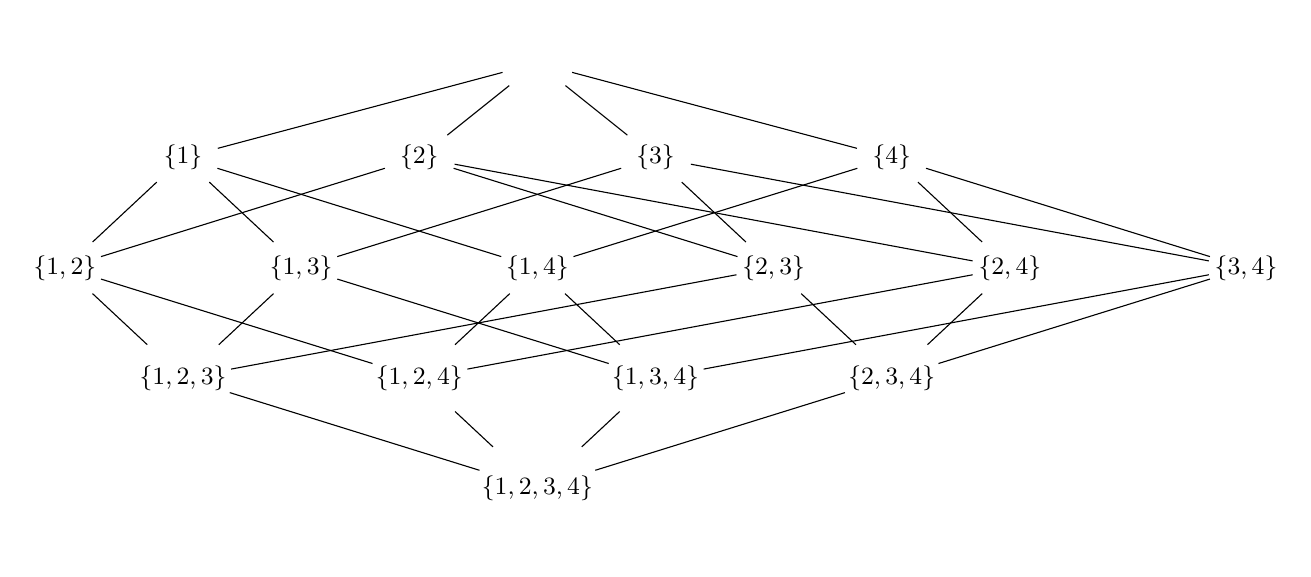
\begin{tikzpicture}[
                every node/.style={inner sep=1pt, font=\small},
                lvl/.style={yshift=#1},
                dot/.style={circle, minimum size=9mm},
                >=stealth
            ]
            % لایه 0
            \node[dot] (e) {$\varnothing$};

            % لایه 1
            \node[dot, lvl=-1.2cm, xshift=-4.5cm] (1) {$\{1\}$};
            \node[dot, lvl=-1.2cm, xshift=-1.5cm] (2) {$\{2\}$};
            \node[dot, lvl=-1.2cm, xshift= 1.5cm] (3) {$\{3\}$};
            \node[dot, lvl=-1.2cm, xshift= 4.5cm] (4) {$\{4\}$};

            % لایه 2
            \node[dot, lvl=-2.6cm, xshift=-6.0cm] (12) {$\{1,2\}$};
            \node[dot, lvl=-2.6cm, xshift=-3.0cm] (13) {$\{1,3\}$};
            \node[dot, lvl=-2.6cm, xshift= 0.0cm] (14) {$\{1,4\}$};
            \node[dot, lvl=-2.6cm, xshift= 3.0cm] (23) {$\{2,3\}$};
            \node[dot, lvl=-2.6cm, xshift= 6.0cm] (24) {$\{2,4\}$};
            \node[dot, lvl=-2.6cm, xshift= 9.0cm] (34) {$\{3,4\}$};

            % لایه 3
            \node[dot, lvl=-4.0cm, xshift=-4.5cm] (123) {$\{1,2,3\}$};
            \node[dot, lvl=-4.0cm, xshift=-1.5cm] (124) {$\{1,2,4\}$};
            \node[dot, lvl=-4.0cm, xshift= 1.5cm] (134) {$\{1,3,4\}$};
            \node[dot, lvl=-4.0cm, xshift= 4.5cm] (234) {$\{2,3,4\}$};

            % لایه 4
            \node[dot, lvl=-5.4cm] (1234) {$\{1,2,3,4\}$};

            % یال‌ها (روابط پوشا)


            \draw (e) -- (1) (e) -- (2) (e) -- (3) (e) -- (4);

            \draw (1) -- (12) (1) -- (13) (1) -- (14);
            \draw (2) -- (12) (2) -- (23) (2) -- (24);
            \draw (3) -- (13) (3) -- (23) (3) -- (34);
            \draw (4) -- (14) (4) -- (24) (4) -- (34);

            \draw (12) -- (123) (12) -- (124);
            \draw (13) -- (123) (13) -- (134);
            \draw (14) -- (124) (14) -- (134);
            \draw (23) -- (123) (23) -- (234);
            \draw (24) -- (124) (24) -- (234);
            \draw (34) -- (134) (34) -- (234);

            \draw (123) -- (1234);
            \draw (124) -- (1234);
            \draw (134) -- (1234);
            \draw (234) -- (1234);
        \end{tikzpicture}
    }
\end{frame}



\begin{frame}[t]{عنصر ماکسیمال}

    \begin{definition}
        فرض کنید $(A,\le)$ یک مجموعهٔ مرتبِ جزئی باشد. عنصری $a\in A$ را \textit{بیشینه (ماکسیمال) در $A$} می‌نامیم هرگاه برای هر $c\in A$ که \textit{با $a$ قابلِ مقایسه} است، داشته باشیم $c\le a$؛ به‌عبارتِ دیگر، برای همهٔ $c\in A$،
        \[
            a \le c \;\Rightarrow\; a = c.
        \]
    \end{definition}



\end{frame}

\begin{frame}[t,fragile]{نمونه‌هایی از عناصر ماکسیمال}
    توجه کنید اگر $a$ بیشینه باشد، الزاماً این‌گونه نیست که برای همهٔ $c\in A$ داشته باشیم $c\le a$ (ممکن است عناصری در $A$ باشند که با $a$ قابلِ مقایسه نباشند). همچنین یک مجموعه ممکن است چندین عنصرِ بیشینه داشته باشد، یا اصلاً هیچ عنصری بیشینه نداشته باشد (برای مثال، $\mathbb{Z}$ با ترتیبِ معمولش).



    \begin{example}
        \centering
        \resizebox{0.78\linewidth}{!}{
            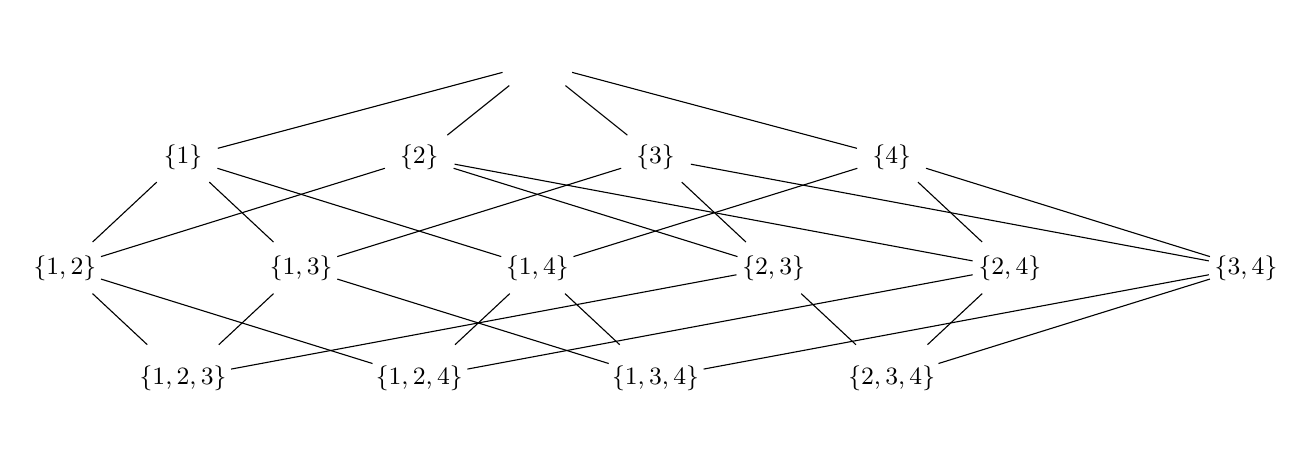
\begin{tikzpicture}[
                    every node/.style={inner sep=1pt, font=\small},
                    lvl/.style={yshift=#1},
                    dot/.style={circle, minimum size=9mm},
                    >=stealth
                ]
                % لایه 0
                \node[dot] (e) {$\varnothing$};

                % لایه 1
                \node[dot, lvl=-1.2cm, xshift=-4.5cm] (1) {$\{1\}$};
                \node[dot, lvl=-1.2cm, xshift=-1.5cm] (2) {$\{2\}$};
                \node[dot, lvl=-1.2cm, xshift= 1.5cm] (3) {$\{3\}$};
                \node[dot, lvl=-1.2cm, xshift= 4.5cm] (4) {$\{4\}$};

                % لایه 2
                \node[dot, lvl=-2.6cm, xshift=-6.0cm] (12) {$\{1,2\}$};
                \node[dot, lvl=-2.6cm, xshift=-3.0cm] (13) {$\{1,3\}$};
                \node[dot, lvl=-2.6cm, xshift= 0.0cm] (14) {$\{1,4\}$};
                \node[dot, lvl=-2.6cm, xshift= 3.0cm] (23) {$\{2,3\}$};
                \node[dot, lvl=-2.6cm, xshift= 6.0cm] (24) {$\{2,4\}$};
                \node[dot, lvl=-2.6cm, xshift= 9.0cm] (34) {$\{3,4\}$};

                % لایه 3
                \node[dot, lvl=-4.0cm, xshift=-4.5cm] (123) {$\{1,2,3\}$};
                \node[dot, lvl=-4.0cm, xshift=-1.5cm] (124) {$\{1,2,4\}$};
                \node[dot, lvl=-4.0cm, xshift= 1.5cm] (134) {$\{1,3,4\}$};
                \node[dot, lvl=-4.0cm, xshift= 4.5cm] (234) {$\{2,3,4\}$};

                % یال‌ها (روابط پوشا)


                \draw (e) -- (1) (e) -- (2) (e) -- (3) (e) -- (4);

                \draw (1) -- (12) (1) -- (13) (1) -- (14);
                \draw (2) -- (12) (2) -- (23) (2) -- (24);
                \draw (3) -- (13) (3) -- (23) (3) -- (34);
                \draw (4) -- (14) (4) -- (24) (4) -- (34);

                \draw (12) -- (123) (12) -- (124);
                \draw (13) -- (123) (13) -- (134);
                \draw (14) -- (124) (14) -- (134);
                \draw (23) -- (123) (23) -- (234);
                \draw (24) -- (124) (24) -- (234);
                \draw (34) -- (134) (34) -- (234);


            \end{tikzpicture}
        }


    \end{example}

    \begin{example}
        \centering
        
\begin{tikzpicture}[>=stealth, scale=0.9, transform shape]
            % points:  ... -3, -2, -1, 0, 1, 2, 3 ...
            \node (dotsL) at (-6.2,0) {$\cdots$};
            \node[circle, draw, minimum size=7mm, inner sep=1pt] (m3) at (-4.5,0) {$-3$};
            \node[circle, draw, minimum size=7mm, inner sep=1pt] (m2) at (-3.0,0) {$-2$};
            \node[circle, draw, minimum size=7mm, inner sep=1pt] (m1) at (-1.5,0) {$-1$};
            \node[circle, draw, minimum size=7mm, inner sep=1pt] (z0) at (0,0) {$0$};
            \node[circle, draw, minimum size=7mm, inner sep=1pt] (p1) at (1.5,0) {$1$};
            \node[circle, draw, minimum size=7mm, inner sep=1pt] (p2) at (3.0,0) {$2$};
            \node[circle, draw, minimum size=7mm, inner sep=1pt] (p3) at (4.5,0) {$3$};
            \node (dotsR) at (6.2,0) {$\cdots$};

            % cover relations (arrows point to the greater element)
            \begin{scope}[->]
                \draw (m3) -- (m2);
                \draw (m2) -- (m1);
                \draw (m1) -- (z0);
                \draw (z0) -- (p1);
                \draw (p1) -- (p2);
                \draw (p2) -- (p3);
            \end{scope}
        \end{tikzpicture}
    \end{example}


\end{frame}


\begin{frame}[t]{کران بالا و زنجیر}
    \begin{definition}
        یک \textit{کران بالا} برای زیرمجموعه‌ای ناتهی $B$ از $A$ عنصری $d \in A$ است به‌طوری‌که
        \[
            \forall b \in B; \quad b \le d
        \]


    \end{definition}

    \begin{definition}
        زیرمجموعهٔ ناتهی $B$ از $A$ که به‌وسیلهٔ رابطهٔ $\le$ به‌صورت خطی مرتب شده باشد، یک \textit{زنجیر در $A$} نامیده می‌شود.
    \end{definition}



\end{frame}

\begin{frame}[t]{لم زورن}

    \begin{definition}[لم زورن ]
        اگر $A$ یک مجموعهٔ مرتبِ جزئیِ ناتهی باشد به‌طوری‌که هر زنجیر در $A$ دارای کرانِ بالا در $A$ باشد، آنگاه $A$ دارای عنصری بیشینه است.
    \end{definition}


    با فرضِ این‌که سایر اصولِ موضوعهٔ معمولِ نظریهٔ مجموعه‌ها برقرارند، می‌توان اثبات کرد که لمِ زورن درست است اگر و تنها اگر اصلِ انتخاب برقرار باشد؛ به‌عبارتِ دیگر، این دو با یکدیگر \textit{معادل‌اند.}

\end{frame}
\standout{تمرین}
\begin{frame}[t]{لتیس و کران‌های پایین و بالا}
    \begin{exercise}
        فرض کنید $(A,\le)$ یک مجموعهٔ مرتبِ جزئی باشد و $B$ زیرمجموعه‌ای ناتهی. یک \textit{کرانِ پایین} برای $B$ عنصری $d \in A$ است به‌طوری‌که برای \textit{هر} $b \in B$ داشته باشیم $d \le b$. یک \textit{بزرگ‌ترین کرانِ پایین \lr{(g.l.b.)}} برای $B$ کرانِ پایینی $d_0$ از $B$ است به‌گونه‌ای که برای هر کرانِ پایینِ دیگرِ $d$ از $B$ داشته باشیم $d \le d_0$. یک \textit{کوچک‌ترین کرانِ بالا \lr{(l.u.b.)}} برای $B$ کرانِ بالایی $t_0$ از $B$ است به‌گونه‌ای که برای هر کرانِ بالایِ دیگرِ $t$ داشته باشیم $t_0 \le t$. زوجِ $(A,\le)$ یک \textit{لتیس} است هرگاه برای همۀ $a,b \in A$ مجموعهٔ $\{a,b\}$ هم بزرگ‌ترین کرانِ پایین و هم کوچک‌ترین کرانِ بالا را داشته باشد.

        \begin{enumerate}
            \item اگر $S \ne \emptyset$، آنگاه توانِ مجموعهٔ $\mathcal{P}(S)$ با ترتیبِ شمولِ مجموعه‌ای یک لتیس است که یک عنصرِ بیشینهٔ یکتا دارد.
            \item مثالی از یک مجموعهٔ مرتبِ جزئی بیاورید که \textit{لتیس نباشد}.
            \item مثالی از یک لتیس بدونِ عنصرِ بیشینه و نیز مثالی از یک مجموعهٔ مرتبِ جزئی با دو عنصرِ بیشینه بیاورید.
        \end{enumerate}

    \end{exercise}
\end{frame}

\begin{frame}[t]{لتیس کامل و نقطهٔ ثابت}

    \begin{exercise}
        یک لتیس $(A,\le)$ (بنگرید به تمرین~1) را \textit{کامل} می‌نامیم هرگاه هر زیرمجموعهٔ ناتهی از $A$ هم کوچک‌ترین کرانِ بالا و هم بزرگ‌ترین کرانِ پایین را داشته باشد.
        تابعی میان مجموعه‌های مرتبِ جزئی $f\colon A \to B$ را \textit{حافظِ ترتیب} می‌نامیم هرگاه از $a \le a'$ در $A$ نتیجه شود که $f(a) \le f(a')$ در $B$.
        اثبات کنید که یک تابعِ حافظِ ترتیب $f$ از یک لتیس کاملِ $A$ به خودش، دست‌کم یک عنصرِ ثابت دارد (یعنی عنصری $a \in A$ که $f(a)=a$).

    \end{exercise}

    \begin{exercise}
        یک ترتیبِ خوش‌ترتیب بر مجموعهٔ اعدادِ گویا $\mathbb{Q}$ ارائه دهید.

    \end{exercise}
\end{frame}



\begin{frame}[t]{تابع انتخاب و ترتیب در صفحه}
    \begin{exercise}
        فرض کنید $S$ یک مجموعه باشد. یک \textit{تابعِ انتخاب برای $S$} تابعی است
        \( f \) از مجموعهٔ تمام زیرمجموعه‌های ناتهیِ $S$ به $S$، یعنی
        \[
            f:\{\,A \subseteq S \mid A \neq \emptyset\,\}\longrightarrow S,
        \]
        به‌طوری‌که برای هر \( A \neq \emptyset \) با \( A \subseteq S \) داشته باشیم \( f(A)\in A \).
        نشان دهید که «اصلِ انتخاب» معادلِ این گزاره است که هر مجموعهٔ \( S \) دارای یک تابعِ انتخاب است.

    \end{exercise}

\end{frame}

\begin{frame}[t]{ترتیبی با بی‌نهایت عنصر ماکسیمال}
    \begin{exercise}
        فرض کنید $S$ مجموعهٔ همهٔ نقاط $(x,y)$ در صفحه باشد که $y \le 0$. ترتیبی به‌صورت
        \[
            (x_1,y_1) \le (x_2,y_2) \;\Leftrightarrow\; x_1 = x_2 \ \text{و}\ y_1 \le y_2
        \]
        تعریف می‌کنیم. نشان دهید که این یک ترتیبِ جزئی بر $S$ است و این‌که $S$ بی‌نهایت عنصرِ بیشینه دارد.

    \end{exercise}


\end{frame}


\fi
\end{document}
